\documentclass[a4paper, twoside, 12pt]{report}
\usepackage{vntex}
% \usepackage[english,vietnam]{babel}
\usepackage[utf8]{inputenc}

% \usepackage[utf8]{inputenc}
% %\usepackage[francais]{babel}
\usepackage{a4wide,amssymb,epsfig,latexsym,array,hhline,fancyhdr}
\usepackage[normalem]{ulem}
\usepackage{soul}
\usepackage{tabto}
\usepackage[makeroom]{cancel}
\usepackage{amsmath}
\usepackage{amsthm}
\usepackage{multicol,longtable,amscd}
\usepackage{diagbox}%Make diagonal lines in tables
\usepackage{booktabs}
\usepackage{alltt}
\usepackage[framemethod=tikz]{mdframed}% For highlighting paragraph backgrounds
\usepackage{caption,subcaption}

\usepackage{lastpage}
\usepackage[lined,boxed,commentsnumbered]{algorithm2e}
\usepackage{enumerate}
\usepackage{color}
\usepackage{graphicx}							% Standard graphics package
\usepackage{array}
\usepackage{tabularx, caption}
\usepackage{multirow}
\usepackage{multicol}
\usepackage{rotating}
\usepackage{graphics}
\usepackage{geometry}
\usepackage{setspace}
\usepackage{epsfig}
\usepackage{tikz}
\usepackage{afterpage}
\usepackage{times}
\usetikzlibrary{arrows,snakes,backgrounds}
\usepackage[unicode]{hyperref}
\hypersetup{urlcolor=blue,linkcolor=black,citecolor=black,colorlinks=true} 
%\usepackage{pstcol} 								% PSTricks with the standard color package

\usepackage[normalem]{ulem}
\usepackage{multirow}
\usepackage{listings}

\usepackage{graphicx}
\usepackage{wrapfig}

\usepackage{tocbibind} % Sử dụng gói lệnh tocbibind

\lstdefinestyle{myStyle}{
    belowcaptionskip=1\baselineskip,
    breaklines=true,
    frame=none,
    numbers=none,
    basicstyle=\footnotesize\ttfamily,
    keywordstyle=\bfseries\color{green!40!black},
    commentstyle=\itshape\color{purple!40!black},
    identifierstyle=\color{blue},
    backgroundcolor=\color{gray!10!white},
}
\lstset{style=myStyle}

\newtheorem{theorem}{{\bf Định lý}}
\newtheorem{property}{{\bf Tính chất}}
\newtheorem{proposition}{{\bf Mệnh đề}}
\newtheorem{corollary}[proposition]{{\bf Hệ quả}}
\newtheorem{lemma}[proposition]{{\bf Bổ đề}}
\theoremstyle{definition}
\newtheorem{exer}{Bài toán}

\def\thesislayout{	% A4: 210 × 297
	\geometry{
		a4paper,
		total={160mm,240mm},  % fix over page
		left=3cm,
		top=3cm,
		right=2cm,
		bottom=2.5cm, 
	}
}
\thesislayout

\usepackage{fancyhdr}
\pagestyle{fancy}
\setlength{\headheight}{100pt}
\fancyhead{}
\fancyhead[L]{\leftmark}

\fancyfoot{} % clear all footer fields
\fancyfoot[L]{\scriptsize \ttfamily Đồ án tốt nghiệp}
\fancyfoot[R]{\scriptsize \ttfamily Trang {\thepage}/\pageref{LastPage}}
\renewcommand{\headrulewidth}{0.3pt}
\renewcommand{\footrulewidth}{0.3pt}

% %%%
\setcounter{secnumdepth}{4}
\setcounter{tocdepth}{3}
\makeatletter
\newcounter {subsubsubsection}[subsubsection]
\renewcommand\thesubsubsubsection{\thesubsubsection .\@alph\c@subsubsubsection}
\newcommand\subsubsubsection{\@startsection{subsubsubsection}{4}{\z@}%
                                     {-3.25ex\@plus -1ex \@minus -.2ex}%
                                     {1.5ex \@plus .2ex}%
                                     {\normalfont\normalsize\bfseries}}
\newcommand*\l@subsubsubsection{\@dottedtocline{3}{10.0em}{4.1em}}
\newcommand*{\subsubsubsectionmark}[1]{}
\makeatother

\everymath{\color{black}}%make in-line maths symbols blue to read/check easily

\sloppy
\captionsetup[figure]{labelfont={small,bf},textfont={small,it},belowskip=-1pt,aboveskip=-9pt}
%space remove between caption, figure, and text
\captionsetup[table]{labelfont={small,bf},textfont={small,it},belowskip=-1pt,aboveskip=7pt}

\setlength{\floatsep}{5pt plus 2pt minus 2pt}
\setlength{\textfloatsep}{5pt plus 2pt minus 2pt}
\setlength{\intextsep}{10pt plus 2pt minus 2pt}

\thesislayout

\newcommand\blankpage{%
    \null
    \thispagestyle{empty}%
    \addtocounter{page}{-1}%
    \newpage}
\newcommand{\setupfont}[1]{\fontsize{#1}{#1}\selectfont}
\DeclareMathOperator*{\argmax}{arg\,max}
\DeclareMathOperator*{\argmin}{arg\,min}

\newcommand{\norm}[1]{\lVert #1 \rVert}
\newcommand{\bignorm}[1]{\bigg \lVert #1 \bigg \rVert}

\newcommand{\recomplex}[1]{#1}
\newcommand{\imcomplex}[1]{#1i}
\newcommand{\complex}[2]{#1 + i#2}
\newcommand{\polarcomplex}[2]{#1e^{#2i}}
\newcommand{\tricomplex}[2]{\cos(#1) + i\sin(#2)}

\newcommand{\cartesiancoord}{Oft}
\newcommand{\complexcoord}{O \Re \Im}

\newcommand{\ifc}{\text{nếu }}
\newcommand{\otherwise}{\text{các trường hợp khác}}

\newcommand{\scalemath}[2]{\scalebox{#1}{\mbox{\ensuremath{\displaystyle #2}}}}

\newcommand{\definition}[1]{\textbf{\textit{#1}}}

\newcommand{\formularef}[1]{(\ref{#1})}
\newcommand{\enumentry}[1]{\textit{#1}}
\newcommand{\name}[1]{\text{#1}}

\newcommand{\figref}[1]{Hình~\ref{#1}}
\newcommand{\tableref}[1]{Bảng~\ref{#1}}
\newcommand{\labelref}[2]{#1~\ref{#2}}


\newcommand{\chapterref}[1]{Chương~\ref{#1}}
\newcommand{\sectionref}[1]{Mục~\ref{#1}}
\newcommand{\subsectionref}[1]{Tiểu mục~\ref{#1}}
\newcommand{\appendixref}[1]{Phụ lục~\ref{#1}}

\newcommand{\urlsrc}[1]{(nguồn~\url{#1})}
\newcommand{\citesrc}[1]{(nguồn~\cite{#1})}

\newcommand{\srccaption}[2]{\caption[#1]{#1 #2}}

\newcommand{\numberedeq}{\addtocounter{equation}{1}\tag{\theequation}}
\newcommand{\bigO}{\name{O}}

\newcommand{\Waveform}{\text{Waveform}}
\newcommand{\Spectrum}{\text{Spectrum}}
\newcommand{\Spectrogram}{\text{Spectrogram}}

\newcommand{\waveform}{\text{waveform}}
\newcommand{\spectrum}{\text{spectrum}}
\newcommand{\spectrogram}{\text{spectrogram}}
\newcommand\Tstrut{\rule{0pt}{2.6ex}}       % "top" strut
\newcommand\Bstrut{\rule[-0.9ex]{0pt}{0pt}} % "bottom" strut
\newcommand{\TBstrut}{\Tstrut\Bstrut} % top&bottom struts
\newcommand{\subsub}[1]{\noindent \textbf{#1}.}

% \newcommand{\theorem}{Theorem}

\usepackage{fancyhdr}
\renewcommand{\sectionmark}[1]{\markright{\thesection\ #1}}
\fancypagestyle{fancy}{
	\fancyhf{}
	\renewcommand{\headrulewidth}{0.4pt}
	\renewcommand{\footrulewidth}{0pt}
	\fancyhead[OR]{\bfseries \nouppercase{\rightmark}}
	\fancyhead[EL]{\bfseries \nouppercase{\leftmark}}
	\fancyfoot[OR, EL]{\thepage}
}

\fancypagestyle{plain}{
	\fancyhf{}
	\renewcommand{\headrulewidth}{0pt}
	\renewcommand{\footrulewidth}{0pt}
	\fancyfoot[OR, EL]{\thepage}
}
\fancypagestyle{addpagenumbersforpdfimports}{
	\fancyhead{}
	\renewcommand{\headrulewidth}{0pt}
	\fancyfoot{}
	\fancyfoot[R]{\thepage}
}


\usepackage{tikz}
\usetikzlibrary{calc}
\newcommand\HRule{\rule{\textwidth}{1pt}}

\begin{document}

\tolerance=1
\emergencystretch=\maxdimen
\hyphenpenalty=10000
\hbadness=10000

\setlength{\abovedisplayskip}{-2.5mm}
\setlength{\belowdisplayskip}{0pt}
\setlength{\abovedisplayshortskip}{-2.5mm}
%\setlength{\belowdisplayshortskip}{-0.5pt}

\begin{titlepage}
	
\begin{tikzpicture}[remember picture, overlay]
		\draw[line width = 4pt] ($(current page.north west) + (1in + 5,-1in+30)$) rectangle ($(current page.south east) + (-1in+30,1in-20)$);
		\draw[line width = 1pt] ($(current page.north west) + (1in,-1in+35)$) rectangle ($(current page.south east) + (-1in+35,1in-25)$);
	\end{tikzpicture}


	\begin{center}
		\setupfont{14pt}
		ĐẠI HỌC QUỐC GIA THÀNH PHỐ HỒ CHÍ MINH \\
		TRƯỜNG ĐẠI HỌC BÁCH KHOA \\
		KHOA KHOA HỌC VÀ KỸ THUẬT MÁY TÍNH
	\end{center}

	\vspace{1cm}

	\begin{figure}[h!]
		\begin{center}
			
\includegraphics[width=50mm]{img/hcmut.png}
		\end{center}
	\end{figure}


	\begin{center}
		\setupfont{15pt}
		\begin{tabular}{c}
			%       \centering{\textbf{{\Large BÁO CÁO }}}
			%       \newline
			% \multicolumn{1}{l}{\textbf{{\Large ĐỒ ÁN CHUYÊN NGÀNH }}}
			\textbf{{BÁO CÁO}} \\
			\textbf{{ĐỒ ÁN TỐT NGHIỆP}}
		\end{tabular}
	\end{center}

	\vspace*{0.5cm}

	\begin{center}
		\setupfont{17pt}
		\begin{tabular}{c}
			\textbf{{XÂY DỰNG HỆ THỐNG QUẢN LÝ}}    \\
			\textbf{{CỬA HÀNG THỜI TRANG DỰA TRÊN}} \\
			\textbf{{VIỆC TỰ ĐỘNG HÓA QUY TRÌNH NGHIỆP VỤ}}
		\end{tabular}
	\end{center}

	\vspace{0.5cm}


	\begin{center}
		\setupfont{14pt}
		\begin{tabular}{rl}
			\textbf{Ngành:} & Khoa học máy tính
		\end{tabular}
	\end{center}

	% \vspace{1cm}

	\begin{table}[h]
		\setupfont{13pt}
		\begin{tabular}{rll}
			\hspace{5 cm} & \textbf{HỘI ĐỒNG:} & Khoa học Máy tính 21                         \\
			              & \textbf{GVHD:}     & TS. Trương Thị Thái Minh                     \\
			              &                    & TS. Nguyễn An Khương                         \\
			              & \textbf{GVPB:}     & ThS. Phan Trung Hiếu                         \\
			              & \textbf{TKHĐ:}     & TS. Trương Thị Thái Minh                     \\
			              &                    & \multicolumn{1}{c}{\bf---o0o---}\vspace{2mm} \\
			              & \textbf{SVTH 1:}   & Bùi Lương Vinh Hiển - 1913380                \\
			              & \textbf{SVTH 2:}   & Trần Tuấn Phong - 1914641                    \\
			              & \textbf{SVTH 3:}   & Trần Nguyễn Hữu Thọ - 1915347                \\
		\end{tabular}
	\end{table}

	\begin{center}
		{\setupfont{12pt} Thành phố Hồ Chí Minh, 05/2023}
	\end{center}
\end{titlepage}

\setupfont{13pt}

\clearpage
\thispagestyle{empty}
\hfill
\clearpage


\setlength{\parskip}{2.5mm}
\thispagestyle{plain}
\begin{center}
	\section*{Lời cam đoan}
	\addcontentsline{toc}{chapter}{Lời cam đoan}
\end{center}

Nhóm xin cam đoan đây là công trình nghiên cứu của riêng nhóm dưới sự hướng dẫn của TS. Trương Thị Thái Minh, TS. Nguyễn An Khương. Nội dung phân tích và thiết kế hệ thống của nhóm đều là trung thực. Các lý thuyết được sử dụng cho quá trình phân tích, xây dựng được chính nhóm thu thập từ nhiều nguồn khác nhau và sẽ được ghi rõ trong phần tài liệu tham khảo. Ngoài ra, nhóm cũng có sử dụng một số nhận xét, đánh giá và số liệu của các tác giả khác, cơ quan tổ chức khác. Tất cả đều có trích dẫn và chú thích nguồn gốc. Nếu phát hiện có bất kì sự gian lận nào, nhóm xin hoàn toàn chịu trách nhiệm về nội dung đồ án tốt nghiệp của mình. Trường đại học Bách Khoa thành phố Hồ Chí Minh không liên quan đến những vi phạm tác quyền, bản quyền do nhóm gây ra trong quá trình thực hiện.

\vspace{1cm}

\begin{center}
	\begin{tabular}{c c c}
		KÝ TÊN: \rule{4cm}{0.15mm} & \hspace{4cm} & NGÀY: \rule{4cm}{0.15mm} \\ \\
		KÝ TÊN: \rule{4cm}{0.15mm} & \hspace{4cm} & NGÀY: \rule{4cm}{0.15mm} \\ \\
		KÝ TÊN: \rule{4cm}{0.15mm} & \hspace{4cm} & NGÀY: \rule{4cm}{0.15mm}
	\end{tabular}
\end{center}
\setlength{\parskip}{0mm}

\newpage

\setlength{\parskip}{2.5mm}
\thispagestyle{plain}
\begin{center}
	\section*{Lời cảm ơn}
	\addcontentsline{toc}{chapter}{Lời cảm ơn}
\end{center}

Nhóm xin gửi lời cảm ơn sâu sắc đến giáo viên hướng dẫn - Cô Trương Thị Thái Minh, người đã tận tâm hướng dẫn, theo dõi và hỗ trợ nhóm trong suốt quá trình thực hiện đồ án tốt nghiệp. Ngoài những lời khuyên và kiến thức về chuyên môn, trong quá trình làm việc cùng với cô, nhóm còn học được những đức tính tốt, những kỹ năng cần thiết để trở một người làm khoa học thực thụ như khả năng tư duy phản biện, tư duy sáng tạo, sự cần cù, sự trung thực và sự cẩn thận chính xác.

Bên cạnh đó, nhóm xin gửi lời cám ơn chân thành đến Thầy Nguyễn An Khương đã cùng tham gia hướng dẫn, hỗ trợ nhóm thực hiện đồ án tốt nghiệp này trong suốt thời gian vừa qua. Những kiến thức và kinh nghiệm quý báu của thầy đã giúp nhóm rất nhiều trong việc hoàn thiện đồ án tốt nghiệp.

Cuối cùng, nhóm xin gửi lời cám ơn đến quý thầy cô trong Khoa Khoa học và Kỹ thuật Máy tính đã dạy dỗ và truyền đạt những kiến thức quý báu cho các thành viên suốt những năm qua. Những kiến thức, bài học ấy không chỉ giúp nhóm hoàn thiện đồ án tốt nghiệp, mà còn là hành trang vô giá cho mỗi thành viên trong sự nghiệp sau này.

\hspace{10cm} Trân trọng,

\hspace{9cm} Nhóm thực hiện đề tài.

\newpage

\setlength{\parskip}{2.5mm}
\thispagestyle{plain}
\begin{center}
	\section*{Tóm tắt đề tài}
	\addcontentsline{toc}{chapter}{Tóm tắt đề tài}
\end{center}

"Hệ thống quản lý cửa hàng thời trang dựa trên tự động hóa quy trình nghiệp vụ" là một hệ thống ứng dụng web được tích hợp BPEL nhằm hỗ trợ việc quản lý các quy trình nghiệp vụ. Hệ thông nhằm cho thấy được sự tối ưu về thời gian và nhân lực trong các quá trình chuyển đổi các quy trình nghiệp vụ trong nhu cầu tần xuất thay đổi các quy trình nghiệp vụ ngày càng thường xuyên hơn. Để thực hiện hệ thống này, nhóm đã thực hiện các công việc sau:
\begin{itemize}
	\item Tìm hiểu các nghiệp vụ của các hệ thống cửa hàng thời trang
	\item Thiêt kế hệ thống bao gồm các lược đồ usecase, BPMN, lựa chọn kiến trúc, lược đồ class, cơ sở dữ liệu
	\item Tìm hiểu việc chuyển đổi BPMN sang BPEL và tích hợp BPEL vào hệ thống
	\item Thực hiện xây dựng hệ thống và kiểm thử
\end{itemize}



\setlength{\parskip}{0mm}

\tableofcontents

\newpage
\listoffigures
\newpage

\listoftables

\newpage
\textbf{Các cụm từ viết tắt có trong bài:}
{
	\setlength\extrarowheight{6pt}
	\begin{longtable}{| p{4cm} | p{11cm} |}

		\hline
		\textbf{Cụm từ viết tắt} & \textbf{Cụm từ đầy đủ}                              \\
		\hline
		%%%%%%%%%%%%%%%%%%%%%%
		BPM                      & Business Process Management                         \\
		\hline
		%%%%%%%%%%%%%%%%%%%%%%
		BPA                      & Business Process Automation                         \\
		\hline
		%%%%%%%%%%%%%%%%%%%%%%
		BPMN                     & Business Process Management Notations               \\
		\hline
		%%%%%%%%%%%%%%%%%%%%%%
		BPEL                     & Business Process Execution Language                 \\
		\hline
		%%%%%%%%%%%%%%%%%%%%%%
		BPEL4WS                  & Business Process Execution Language for Web Service \\
		\hline
		%%%%%%%%%%%%%%%%%%%%%%
		BAW                      & Business Automation Workflow                        \\
		\hline
		%%%%%%%%%%%%%%%%%%%%%%
		BFF                      & Backend For Frontend                                \\
		\hline
		%%%%%%%%%%%%%%%%%%%%%%
		SEO                      & Search Engine Optimization                          \\
		\hline
		\caption{Các từ viết tắt}
	\end{longtable}

}

%%%%%%%%%%%%%%%%%%%%%%%%%%%%%%%%%%%

% Giới thiệu
\chapter{Tổng quan}
% !TeX root = ..\main.tex
\section{Tổng quan}
%%%%%%%%%%%%%%%%%%%%%%%%%
\subsection{Giới thiệu đề tài}

\hspace{0.5cm}Trong thời đại công nghiệp 4.0 hiện nay, với sự bùng nổ của không gian mạng cùng vai trò ngày càng lớn của dữ liệu thời gian thực, việc áp dụng công nghệ vào quản lý quy trình sản xuất đã mang lại nhiều hiệu quả rất đáng ghi nhận. Việc kết nối vật lý với kỹ thuật số cho phép các bộ phận trong quy trình, bao gồm nhà cung cấp, đối tác, khách hàng và sản phẩm có thể kết nối tốt hơn. Công nghiệp 4.0 đang giúp các công ty, doanh nghiệp có thể dễ dàng hợp tác và chia sẻ dữ liệu giữa các khách hàng, nhà sản xuất, nhà cung cấp và các bên khác trong chuỗi cung ứng. Nó cải thiện năng suất và khả năng cạnh tranh, cho phép chuyển đổi sang nền kinh tế kỹ thuật số và cung cấp cơ hội để đạt được tăng trưởng kinh tế và bền vững. Với những lợi ích trong thời đại công nghiệp 4.0 mang đến như vậy, việc chuyển đổi số của các doanh nghiệp là không thể tránh khỏi. Với khả năng cập nhật dữ liệu nhanh chóng, các nhà quản lý hay chủ doanh nghiệp có thể nắm bắt khía cạnh khác nhau của doanh nghiệp 1 cách nhanh chóng và có thể tìm cách để cải thiện. Mà trong 1 doanh nghiệp khi hoạt động, để đạt được những mục tiêu kinh doanh thì phải trải qua chuỗi các hoạt động khác nhau và đó chính là quy trình nghiệp vụ.\\

Quy trình nghiệp vụ là một thành phần quan trọng trong quá trình hoạt động của doanh nghiệp, nó đảm bảo các hoạt động được thực hiện có trình tự và sẽ đạt được kết quả đúng với mục tiêu. Các quy trình nghiệp vụ đại diện cho một trong những tài sản cốt lõi của các tổ chức vì nhiều lý do khác nhau. Chúng có tác động trực tiếp đến sức hấp dẫn của sản phẩm và dịch vụ, ảnh hưởng đến trải nghiệm của khách hàng và cuối cùng là ảnh hưởng đến doanh thu của doanh nghiệp. Các quy trình phối hợp các nguồn lực của công ty để đáp ứng các nhu cầu bên ngoài này, do đó các quy trình này là yếu tố chính xác định chi phí để phục vụ và hoạt động hiệu quả. Cụ thể, chúng xác định các nhiệm vụ, công việc và trách nhiệm, bằng cách này, ta có thể định hình công việc trong tương lai của mọi nhân viên và máy móc trong quy trình kinh nghiệp. Các quy trình là hệ thống quan trọng trong tổ chức và trong mạng lưới cung ứng liên tổ chức. Do đó, bất kỳ lỗi quy trình nào cũng có thể khiến hoạt động của công ty và toàn bộ hệ sinh thái bị đình trệ. Các quy trình xác định tiềm năng và tốc độ của một tổ chức để thích ứng với hoàn cảnh mới và tuân thủ số lượng yêu cầu lập pháp đang tăng lên nhanh chóng.\\

Nhu cầu ngày càng tăng về toàn cầu hóa, tích hợp, tiêu chuẩn hóa, đổi mới, nhanh nhẹn và hoạt động hiệu quả, cùng với các cơ hội do công nghệ kỹ thuật số mang lại, cuối cùng đã làm tăng nhu cầu cải thiện  cũng như thiết kế toàn bộ quy trình nghiệp vụ mới. Một bộ công cụ, kỹ thuật và phương pháp được sinh ra để hỗ trợ tất cả các giai đoạn của vòng đời quy trình nghiệp vụ đã xuất hiện trong hai thập kỷ qua. Nó được gọi là "Quy trình quản lý nghiệp vụ (BPM)". BPM hợp nhất rất nhiều công cụ và cách tiếp cận đến từ nhiều lĩnh vực khác nhau, bao gồm kỹ thuật công nghiệp, quản lý hoạt động, quản lý chất lượng, quản lý nguồn nhân lực, quản trị doanh nghiệp, khoa học máy tính và kỹ thuật, hệ thống thông tin.\\

Khi các quy trình nghiệp vụ đã được xây dựng và được thực hiện, thì trong quá hình hiện thực có thể xảy ra sai sót bởi con người hay những quy trình có thể cần được cải thiện và khi sửa đổi quy trình, doanh nghiệp cần tiêu tốn rất nhiều thời gian cũng như nguồn lực để xây dựng lại ứng dụng điều phối quy trình. Từ đây, nhu cầu áp dụng công nghệ vào việc tự động hóa các quy trình được sinh ra. \textbf{Tự động hóa quy trình nghiệp vụ (BPA)} là việc sử dụng phần mềm để tự động hóa các giao dịch kinh doanh nhiều bước, có thể lặp lại. Trái ngược với các loại tự động hóa khác, các giải pháp BPA có xu hướng phức tạp, được kết nối với nhiều hệ thống công nghệ thông tin (CNTT) và được điều chỉnh cụ thể theo nhu cầu của một tổ chức. Các tổ chức thường áp dụng BPA như một phần của chiến lược chuyển đổi kỹ thuật số, nhằm hợp lý hóa quy trình làm việc của họ và hoạt động hiệu quả hơn. Tự động hóa quy trình nghiệp vụ có thể giải phóng thời gian và nguồn lực cho doanh nghiệp rất nhiều.\\

Với các yêu cầu về thiết kế và mô hình hóa quy trình kinh doanh như vậy, mô hình và ký hiệu mô hình hóa quy trình nghiệp vụ (BPMN) là ngôn ngữ hướng đồ thị được sinh ra và cung cấp cho các doanh nghiệp khả năng hiểu các quy trình kinh doanh nội bộ của họ dưới dạng ký hiệu đồ họa và sẽ cung cấp cho các tổ chức khả năng truyền đạt các quy trình này theo cách tiêu chuẩn. Hơn nữa, ký hiệu đồ họa sẽ tạo điều kiện cho sự hiểu biết về hiệu suất hợp tác và giao dịch kinh doanh giữa các tổ chức. Điều này sẽ đảm bảo rằng các doanh nghiệp sẽ hiểu chính họ và những người tham gia vào hoạt động kinh doanh của họ, đồng thời sẽ cho phép các tổ chức điều chỉnh nhanh chóng các tình huống kinh doanh nội bộ và B2B mới. Khi thiết kế và cải thiện quy trình kinh doanh sử dụng BPMN thì đến khi thực hiện, chúng ta cần sử dụng đến BPEL(ngôn ngữ thực thi quy trình doanh nghiệp) thể có thể hiện thực nó, được dùng bởi các lập trình viên và nhà phân tích kỹ thuật. Trong khi BPMN thể hiện các ký hiệu để cho các phía về mặt business đều hiểu thì BPEL lại là ngôn ngữ thực thi để lập trình viên có thể hiện thực những mô tả từ các ký hiệu trong BPMN. Hiện nay có 1 số công cụ hỗ trợ chuyển đổi từ BPMN sang BPEL như Oracle Business Process Analysis Suite. Với các công nghệ và kỹ thuật ở trên thì ta có thể kết hợp lại để thực hiện BPA, khi doanh nghiệp muốn cập nhật hay cải thiện về quy trình kinh doanh thì có thể cập nhật trên các lược đồ BPMN, từ đầu chúng ta có thể sử dụng các công cụ để chuyển đổi thành lược đồ BPEL, sau khi được chuyển đổi thì có thể cập nhật vào hệ thống để hệ thống cập nhật quy trình mới, từ đó tiết kiệm được lượng lớn chi phí khi phải thuê một đội ngũ công nghệ thông tin để cập nhật lại hệ thống khi có thay đổi. Qua các nội dung đã được trình bày ở trên, nhóm sẽ thực hiện áp dụng tự động hóa quy trình nghiệp vụ cho một hệ thống cửa hàng thời trang trong đề tài: "Xây dựng ứng dụng quản lý hệ thống cửa hàng thời trang dựa trên việc tự động hóa quy trình nghiệp vụ".
%%%%%%%%%%%%%%%%%%%%%%%%%

\subsection{Mục tiêu đề tài}
\hspace{0.5cm} Mục tiêu của đề tài là áp dụng tự động hóa quy trình nghiệp vụ vào trong một hệ thống thực tế. Việc vận hành hệ thống cần đảm bảo các yêu cầu và các tính năng đề ra. Về phần quy trình nghiệp vụ, nghiệp vụ của hệ thống được quản lý và tự động hóa bằng phương pháp tự động hóa quy trình nghiệp vụ. Việc thiết kế và cập nhật nghiệp vụ sẽ được thuận tiện và thân thiện với cả người dùng nghiệp vụ lẫn lập trình viên với BPMN và việc cập nhật nghiệp vụ vào hệ thống sẽ được tự động với sự trợ giúp của BPEL.

%%%%%%%%%%%%%%%%%%%%%%%%%
\subsection{Phạm vi đề tài}
\par Phạm vi của đề tài này bao gồm:
\begin{itemize}
	\item Thiết kế và hiện thực một hệ thống bán hàng thời trang, bao gồm các tính năng mua / bán hàng trực tuyến và trực tiếp, và các tính năng quản lý hoạt động của hệ thống bán hàng.
	\item Thiết kế quy trình nghiệp vụ của doanh nghiệp bằng phương pháp tự động hóa quy trình nghiệp vụ, biểu diễn quy trình nghiệp vụ bằng BPMN và thực thi nghiệp vụ bằng BPEL.
	\item Áp dụng BPEL vào việc tự động hóa quy trình nghiệp vụ của hệ thống.
\end{itemize}

%%%%%%%%%%%%%%%%%%%%%%%%%
\subsection{Ý nghĩa đề tài}
\hspace{0.5cm} Trong thực tế, quy trình nghiệp vụ của doanh nghiệp thường lớn và phức tạp, đòi hỏi sự tham gia của nhiều thành phần có các mối liên hệ phức tạp với nhau. Một sự thay đổi nghiệp vụ đòi hỏi nhiều thời gian và công sức để áp dụng vào hệ thống thực tế. Đối với phần lập trình và phát triển hệ thống, lập trình viên cần thay đổi mã nguồn ở nhiều nơi để đáp ứng đúng với thay đổi của nghiệp vụ, và cần đảm bảo sau khi thay đổi hệ thống vừa chạy đúng với nghiệp vụ mới, vừa đáp ứng các yêu cầu chức năng và phi chức năng đã đặt ra từ đầu. Với cách tiếp cận này, việc thay đổi và cập nhật quy trình nghiệp vụ sẽ tốn nhiều thời gian khi phải thay đổi mã nguồn ở nhiều phần trong hệ thống, sẽ tốn công sức để đảm bảo hệ thống đáp ứng đúng như yêu cầu sau cập nhật, và dễ có rủi ro nếu việc tìm và thay đổi mã nguồn vẫn chưa triệt để.

\par Với sự giúp đỡ của việc \textbf{Tự động hóa quy trình nghiệp vụ}, việc quản lý quy trình nghiệp vụ sẽ trở nên dễ dàng hơn rất nhiều. Quy trình nghiệp vụ có thể được biểu diễn dưới dạng mô hình BPMN - một mô hình có thể hiểu được bởi người dùng nghiệp vụ và lập trình viên. Việc thay đổi và cập nhật quy trình nghiệp vụ sẽ được tối ưu và tự động với \textbf{Ngôn ngữ thực thi quy trình doanh nghiệp - BPEL}. Các thành phần của hệ thống tương ứng với các bước trong quy trình nghiệp vụ sẽ được kết nối đến các thành phần của BPEL, do đó khi có sự thay đổi của quy trình nghiệp vụ, chỉ cần cập nhật lại BPEL và BPEL sẽ gọi thứ tự thực thi nghiệp vụ mới theo đúng như nó được cập nhật. Do đó, lập trình viên không cần tìm và sửa mã ở khắp nơi trong mã nguồn, mà chỉ cần cập nhật BPEL và đảm bảo kết nối đúng các thành phần BPEL đến các thành phần trong hệ thống. Do BPEL là một ngôn ngữ thực thi, nó có thể được deploy và chạy, nên khi có sự thay đổi nghiệp vụ ở BPMN và BPEL, việc cập nhật nghiệp vụ sẽ nhanh và tự động mà không yêu cầu nhiều công sức của con người.

%%%%%%%%%%%%%%%%%%%%%%%%%
\subsection{Đóng góp của đề tài}
\hspace{0.5cm} Đề tài mong muốn mang đến một cách tiếp cận hiệu quả cho việc thiết kế và quản lý quy trình trong mỗi doanh nghiệp. Sau khi hoàn thành, đề tài muốn cho thấy cách tiếp cận bằng tự động hóa quy trình nghiệp vụ sẽ giảm đáng kể thời gian và nguồn lực trong việc quản lý quy trình nghiệp vụ, và sẽ mang lại hiệu quả lớn cho doanh nghiệp trong việc vận hành hệ thống của mình.

%%%%%%%%%%%%%%%%%%%%%%%%%   
\subsection{Phân chia công việc}
{
\setlength\extrarowheight{6pt}
\begin{longtable}{| p{2cm} | p{2cm} | p{4cm} | p{7cm}|}

	\hline
	\textbf{Bắt đầu} & \textbf{Hạn} & \textbf{Công việc}& \textbf{Phân công} \\
	\hline
	29/08/2022 & 11/09/2022 & 
	- Tìm hiểu về mục tiêu, phạm vi đề tài.
	\newline 
	- Tìm hiểu các lý thuyết liên quan (BPMN, BPEL, chuyển đổi BPMN thành BPEL). & Tất cả thành viên\\
	\hline
	12/09/2022 & 18/09/2022 & 
	- Xác định phạm vi đề tài
	\newline 
	- Phân tích yêu cầu hệ thống. & Tất cả thành viên \\
	\hline
	19/09/2022 & 02/10/2022 & 
	- Chỉnh sửa yêu cầu hệ thống.
	\newline
	- Tiếp tục tìm hiểu về BPMN và BPEL.
	\newline
	- Thiết kế lược đồ BPMN. & 
	- Hiển: Vẽ BPMN cho các tính năng quản lý chi nhánh, quản lý nhân viên, quản lý hoạt động kinh doanh, tính năng cho khách hàng 
	\newline
	- Phong: Vẽ BPMN cho các tính năng quản lý sự kiện, hoạt động bán hàng trực tuyến
	\newline
	- Thọ: Vẽ BPMN cho các tính năng quản lý hàng hóa, quản lý các đơn hàng \\
	\hline
	03/09/2022 & 16/10/2022 & 
	- Xác định use-case, viết đặc tả và vẽ lược đồ use-case. & 
	- Hiển: Vẽ use-case cho quản lý chi nhánh, quản lý nhân viên, quản lý hoạt động kinh doanh, tính năng cho khách hàng 
	\newline
	- Phong: Vẽ use-case cho quản lý sự kiện, hoạt động bán hàng trực tuyến
	\newline
	- Thọ: Vẽ use-case cho quản lý hàng hóa, quản lý các đơn hàng  \\
	\hline
	17/10/2022 & 23/10/2022 & 
	- Thiết kế giao diện hệ thống & 
	- Hiển: Thiết kế giao diện cho quản trị viên
	\newline
	- Phong: Thiết kế giao diện cho khách hàng
	\newline
	- Thọ: Thiết kế giao diện cho quản trị viên
	\\
	\hline
	24/10/2022 & 30/10/2022 & 
	- Tiếp tục thiết kế giao diện.
	\newline
	- Tìm hiểu và lựa chọn kiến trúc hệ thống & Tất cả thành viên tìm hiểu các kiến trúc hệ thống \\
	\hline
	31/10/2022 & 06/11/2022 & 
	- Xây dựng kiến trúc hệ thống
	\newline
	- Phân tích, thu thập các yêu cầu về database.
	\newline
	- Thiết kế ERD, EERD.
	\newline
	- Chỉnh sửa giao diện hệ thống & 
	- Hiển: Thiết kế ERD,EERD cho quản lý chi nhánh, quản lý nhân viên, quản lý hoạt động kinh doanh, tính năng cho khách hàng 
	\newline
	- Phong:Thiết kế ERD,EERD cho quản lý sự kiện, hoạt động bán hàng trực tuyến
	\newline
	- Thọ: Thiết kế ERD,EERD cho quản lý hàng hóa, quản lý các đơn hàng\\
	\hline
	07/11/2022 & 20/11/2022 & Chỉnh sửa kiến trúc hệ thống 
	\newline
	- Thiết kế lược đồ class &
	- Hiển: Thiết kế lược đồ class cho quản lý chi nhánh, quản lý nhân viên, quản lý hoạt động kinh doanh, tính năng cho khách hàng 
	\newline
	- Phong: Thiết kế lược đồ class cho quản lý sự kiện, hoạt động bán hàng trực tuyến
	\newline
	- Thọ: Thiết kế lược đồ class cho quản lý hàng hóa, quản lý các đơn hàng \\
	\hline
	21/11/2022 & 19/12/2022 &  
	- Kiểm duyệt lại toàn bộ hệ thống và viết báo cáo
	\newline
	- Tìm hiểu công nghệ hiện thực hệ thống &
	Tất cả thành viên xem xét hệ thống và làm báo cáo\\
	\hline

\end{longtable}
}

% %%%%%%%%%%%%%%%%%%%%%%%%%%%%%%%%%%%%

%% Cơ sở lý thuyết
\chapter{Cơ sở lý thuyết}
% !TeX root = ..\main.tex
\section{Lược đồ BPMN}
\subsection{Tổng quan về BPMN}
\hspace*{0.5cm}BPMN là một lược đồ tập hợp các kí hiệu để mô hình hóa trực quan các quy trình nghiệp vụ xử lý. BPMN giúp các doanh nghiệp trực quan hóa các hoạt động và các luồng thông tin để thực hiện quy trình nghiệp vụ.
\begin{figure}[!htp]
    \centering
    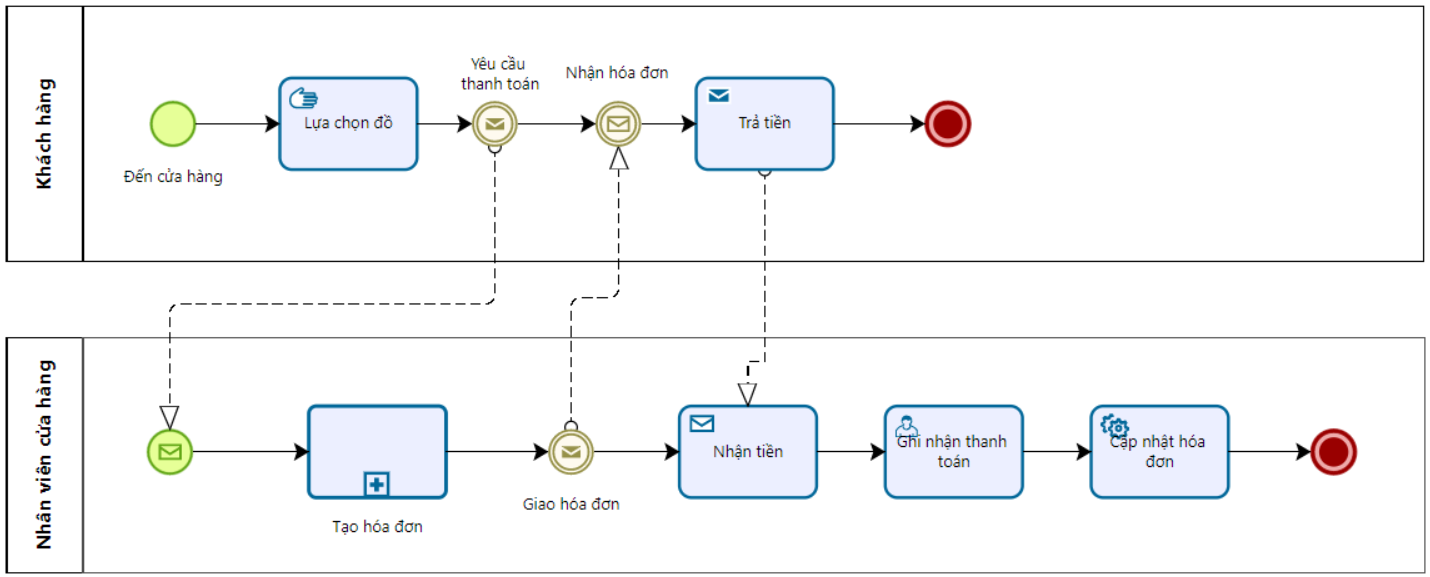
\includegraphics[width=10cm]{img/theory/BPMN/BPMN_sample.png}
    \newline
    \caption{Ví dụ về lược đồ BPMN}
\end{figure}



\subsection{Lợi ích của BPMN}
\begin{itemize}
    \item Giúp các bên liên quan có thể hiểu rõ quy trình nghiệp vụ của hệ thống.
    \item Thu hẹp khoảng cách giữa bộ phận kỹ thuật và bộ phận nghiệp vụ.
    \item Dễ dàng mô tả các nghiệp vụ phức tạp.
\end{itemize}

\subsection{Các thành phần của BPMN}
\subsubsubsection*{Swimlane}
Swimlane bao gồm Pool và Lane:
\begin{itemize}
    \item Pool: Đại diện cho một tổ chức, phòng ban, một vai trò hoặc một hệ thống nào đó.
    \item Lane: Đại diện các cá nhân riêng lẻ, người sẽ làm các hoạt động cụ thể.
\end{itemize}
\newpage
\begin{figure}[!htp]
    \centering
    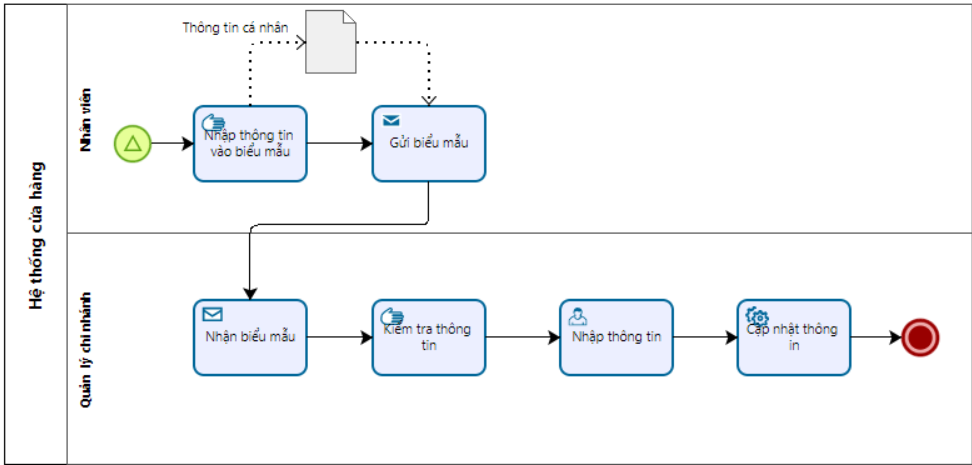
\includegraphics[width=10cm]{img/theory/BPMN/BPMN_swimlane.png}
    \newline
    \caption{Lược đồ BPMN bao gồm 1 pool(Hệ thống cửa hàng) và 2 lane (Nhân viên, Quản lý chi nhánh)}
\end{figure}
\subsubsubsection*{Activities}
Mô tả công việc trong quy trình, được kí hiệu bằng một hình chữ nhật bo tròn 4 góc, bao gồm 4 loại:
\begin{itemize}
    \item Task: Các việc nhỏ, đơn lẻ
          \begin{figure}[!htp]
              \begin{center}
                  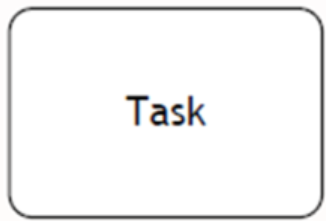
\includegraphics[width=2cm]{img/theory/BPMN/Task.png}
              \end{center}
              \caption{Task \cite{theoryBPMN0}}
          \end{figure}
    \item Event Sub-Process: Một quy trình con nằm trong một quy trình lớn, chức nhiều task
          \begin{figure}[!htp]
              \begin{center}
                  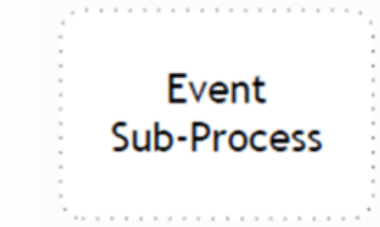
\includegraphics[width=2cm]{img/theory/BPMN/Event Sub-process.png}
              \end{center}
              \caption{Event Sub-Process \cite{theoryBPMN0}}
          \end{figure}
    \item Transaction: Các giao dịch, bao gồm các task nhỏ khác logic với nhau
          \begin{figure}[!htp]
              \begin{center}
                  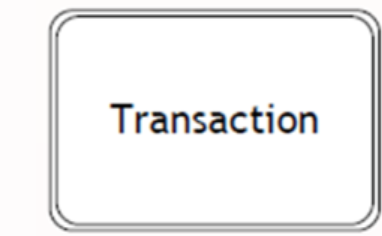
\includegraphics[width=2cm]{img/theory/BPMN/Transaction.png}
              \end{center}
              \caption{Transaction \cite{theoryBPMN0}}
          \end{figure}
    \item Call Activity: Gọi một quy trình khác đã được định nghĩa trong hệ thống, thay vì phải định nghĩa lại nhiều lần
          \begin{figure}[!htp]

              \begin{center}
                  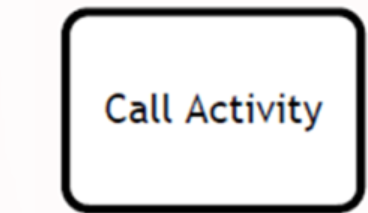
\includegraphics[width=2cm]{img/theory/BPMN/Call Activity.png}
              \end{center}
              \caption{Call Activity \cite{theoryBPMN0}}
          \end{figure}
\end{itemize}


\subsubsubsection*{Events}
Sự kiện là một tác động đến quy trình nghiệp vụ có thể là bên ngoài hoặc bên trong. Các sự kiện thường được kí hiệu bằng hình tròn, bên trong có các kí hiệu về loại hình kích hoạt. Bao gồm các loại:
\begin{itemize}
    \item Start: Các sự kiện mở đầu quy trình nghiệp vụ
    \item Intermediate: Các sự kiện xảy ra giữa các quy trình nghiệp vụ
    \item End: Các sự kiện kết thúc quy trình nghiệp vụ
\end{itemize}
\begin{figure}[!htp]
    \begin{center}
        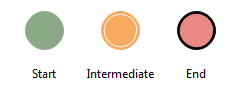
\includegraphics[width=6cm]{img/theory/BPMN/Event.png}
    \end{center}
    \caption{Các loại sự kiện trong BPMN \cite{theoryBPMN1}}
\end{figure}


\subsubsubsection*{Gateways}
Các cổng có nhiệm vụ chính là kiểm soát dòng chảy của quy trình nghiệp vụ. Cổng thường kí hiệu hình thoi, bên trong là ký hiệu các loại.
\begin{itemize}
    \item Start: Các sự kiện mở đầu quy trình nghiệp vụ
    \item Intermediate: Các sự kiện xảy ra giữa các quy trình nghiệp vụ
    \item End: Các sự kiện kết thúc quy trình nghiệp vụ
\end{itemize}
\begin{figure}[!htp]
    \begin{center}
        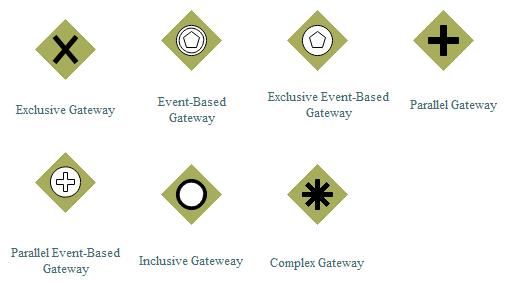
\includegraphics[width=8cm]{img/theory/BPMN/Gateway.png}
    \end{center}
    \caption{Các loại cổng phổ biến trong BPMN \cite{theoryBPMN1}}
\end{figure}



%%%%%%%%%%%%%%%%%%%%%%%%%%%%%%%%%
\section{Ngôn ngữ BPEL}
\subsection{Tổng quan về BPEL}
\hspace*{0.5cm} BPEL hay BPEL4WS là ngôn ngữ dùng để định nghĩa và thực thi các quy trình nghiệp vụ sử dụng các dịch vụ web. Ngôn ngữ BPEL được xây dựng dựa trên nền tảng XML hỗ trợ các dịch vụ web: SOAP, WSDL, UDDI. BPEL xây dựng một dịch vụ web dựa trên việc điều phối, phối hợp các dịch vụ web độc lập khác để hình thành nên một dịch vụ web mới.
\subsection{Các thành phần trong BPEL}
\hspace*{0.5cm}BPEL bao gồm các thành phần nguyên tố và các thành phần cấu trúc. Các thành phần nguyên tố bao gồm:
\begin{itemize}
    \item $<invoke/>$: Gọi một dịch vụ web khác
    \item $<receive/>$: Đợi phản hồi tự các tác vụ bất đồng bộ
    \item $<reply/>$: Phản hồi cho các tác vụ đồng bộ
    \item $<assign/>$: Gán giá trị cho biến
    \item $<throw/>$: Chỉ định các lỗi, ngoại lệ
    \item $<wait/>$: Đợi một thời gian
    \item $<exit/>$: Kết thúc toàn bộ quy trình
\end{itemize}

Bên cạnh thành nguyên tố, các thành phần cấu trúc chứa nhiều tác vụ bên trong:
\begin{itemize}
    \item $<sequence/>$: Các tác vụ thực hiện tuần tự
    \item $<flow/>$: Các tác vụ thực hiện song song
    \item $<if/>$: Thực hiện các tác vụ rẽ nhánh
    \item $<while/>$: Thực hiện các vòng lặp
    \item $<forEach/>$: Thực hiện các vòng lặp
    \item $<repeatUntil/>$: Thực hiện các vòng lặp
    \item $<pick/>$: Đợi các nhánh event
\end{itemize}

Ngoài ra, còn có $<partnerLink>$ dùng để xác định các đối tác, các dịch vụ web sử dụng, $<variable>$ để định nghĩa các biến cần thiết trong quy trình


\subsection{Ví dụ về BPEL}

\hspace*{0.5cm} Để hiểu rõ về quy trình được mô tả bằng BPEL, ta xem xét ví dụ về quy trình sắp xếp chuyến đi cho nhân viên \cite{theoryBPEL}. Đầu tiên, chúng ta sẽ kiểm tra hạng vé của nhân viên, giả sử rằng có một dịch vụ web Employee Travel sẽ làm việc này. Sau đó, chúng ta kiểm tra giá vé của hai hãng: American Airlines và Delta Airlines để chọn ra giá vé thấp hơn và trả lại kết quả. Quy trình này được minh họa như sau:

\begin{figure}[!htp]
    \begin{center}
        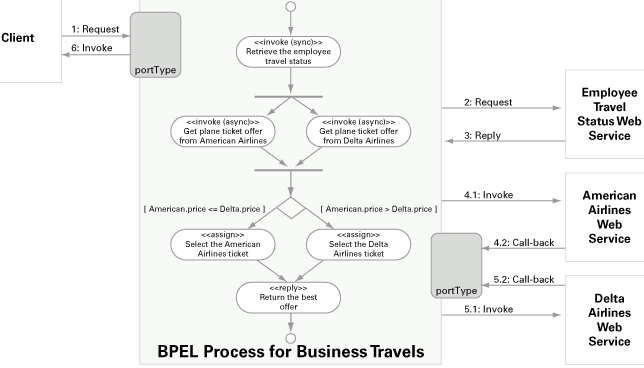
\includegraphics[width=10cm]{img/theory/BPEL/Sample.png}
    \end{center}
    \caption{Ví dụ về quy trình BPEL sắp xếp chuyến đi \cite{theoryBPEL}}
\end{figure}

Trong ví dụ này, các partner của hệ thống bao gồm Client, Employee Travel Status Web Service, American Airlines Web Service, Delta Airlines Web Service. Chúng ta sẽ xây dựng một quy trình BPEL bất đồng bộ, giả định rằng dịch vụ web Employee Travel là đồng bộ vì dữ liệu nhân viên đã có sẵn trong hệ thống chúng ta.

Quy trình BPEL chi tiết như sau. Đầu tiên Client sẽ gửi một yêu cầu bất đồng bộ kèm theo thông tin chuyến đi đến hệ thống. Hệ thống sẽ nhận thông tin và thực hiện lệnh gọi đồng bộ sang dịch vụ web Employee Travel để lấy thông tin hạng vé của nhân viên này. Tiếp theo, hệ thống sẽ thực hiện 2 lệnh gọi bất đồng bộ đồng thời đến 2 dịch vụ web của American Airlines và Delta Airlines để xác định giá vé. Sau khi hệ thống nhận được phản hồi kết quả của 2 hãng hàng không, hệ thống thực hiện so sánh để tìm giá vé thấp hơn và trả lại kết quả cho Client.

\subsection{Các bước xây dựng quy trình BPEL}
Để xây dựng ví dụ trên, ta cần thực hiện các bước sau:
\begin{enumerate}
    \item Xác định các dịch vụ web liên quan: Xác định các dịch vụ web tương tác đối với hệ thống (Employee Travel Web Service, American Airlines Web Service, Delta Airlines Web Service)
    \item Xây dựng WSDL cho quy trình BPEL: BPEL là một dịch vụ web, do đó ta cần xây dựng WSDL cho chính nó
    \item Xác định partnerLink cho quy trình: Cần xác định các dịch vụ web được thực hiện đồng bộ hay bất đồng bộ, cần những tham số nào để gọi.
    \item Xây dựng quy trình: Xây dựng các luồng đi, logic trong quy trình
\end{enumerate}


%%%%%%%%%%%%%%%%%%%%%%%%%%%%%%%%%

\section{Chuyển đổi BPMN sang BPEL}
\hspace*{0.5cm} \par Việc chuyển đổi từ BPMN sang BPEL sẽ giúp tự động hóa quy trình nghiệp vụ. BPMN ở dạng diagram, là mô hình và công cụ để người dùng nghiệp vụ và lập trình viên có thể làm việc và giao tiếp với nhau.
Còn để thực thi được nghiệp vụ, chúng ta cần ngôn ngữ thực thi, ở đây là BPEL. Vậy nên việc chuyển đổi từ BPMN sang BPEL là bước quan trọng trong việc tự động hóa quy trình nghiệp vụ.

\par Đầu tiên, ta đề cập đến các cấu trúc well-structured trong BPMN. Đây là các cấu trúc cơ bản, và dễ dàng để convert sang BPEL, do đó đây sẽ là nền tảng trong việc chuyển đổi. Các cấu trúc well-structured bao gồm:
\begin{itemize}
    \item Sequence
    \item Flow
    \item Switch
    \item Pick
    \item While
    \item Repeat
    \item Repeat - While
\end{itemize}

\par Với các cấu trúc phức tạp hơn, ta gọi các cấu trúc đó là non-well structured. Đối với cấu trúc này, ta có thể chia nhỏ và gom nhóm các thành phần của cấu trúc để tạo nên các well-structured, và từ đó chuyển đổi từng phần well-structured nhỏ sang BPEL.
Sau đó ta gộp các thành phần BPEL đã chuyển đổi để thành BPEL cuối cùng.

\par Giải thuật chuyển đổi từ BPMN X sang BPEL như sau \cite{theoryConvert}:
\begin{enumerate}
    \item Nếu X là well-structured, chuyển đổi trực tiếp sang BPEL, tới bước 4.
    \item Nếu X là non-well structured:
          \begin{enumerate}
              \item Nếu tồn tại thành phần C là Sequence, chọn ra phần đó và đến bước 2.4.
              \item Nếu tồn tại thành phần C là well-structured và non-sequence, chọn ra phần đó và đến bước 2.4.
              \item Nếu tồn tại thành phần C là non-well structured, chọn ra phần đó.
              \item Gán việc ánh xạ C qua BPEL cho công việc t\_{c}.
              \item Quay lại bước 2.
          \end{enumerate}
    \item Xuất ra đoạn code ứng với công việc t\_{c}.
    \item Event nhập và event xuất được ánh xạ tương ứng lần lượt thành <process> và </process> để bao lại phần code BPEL vừa được chuyển đổi.
\end{enumerate}

%%%%%%%%%%%%%%%%%%%%%%%%%%%%%%%%%%%%

\chapter{Thiết kế hệ thống}
% Requirement
\input{tex/Requirement}

\newpage
% Usecase
% !TeX root = ..\main.tex
\section{Lược đồ Use-case}
\subsection{Toàn hệ thống}
\begin{figure}[!htp]
    \centering    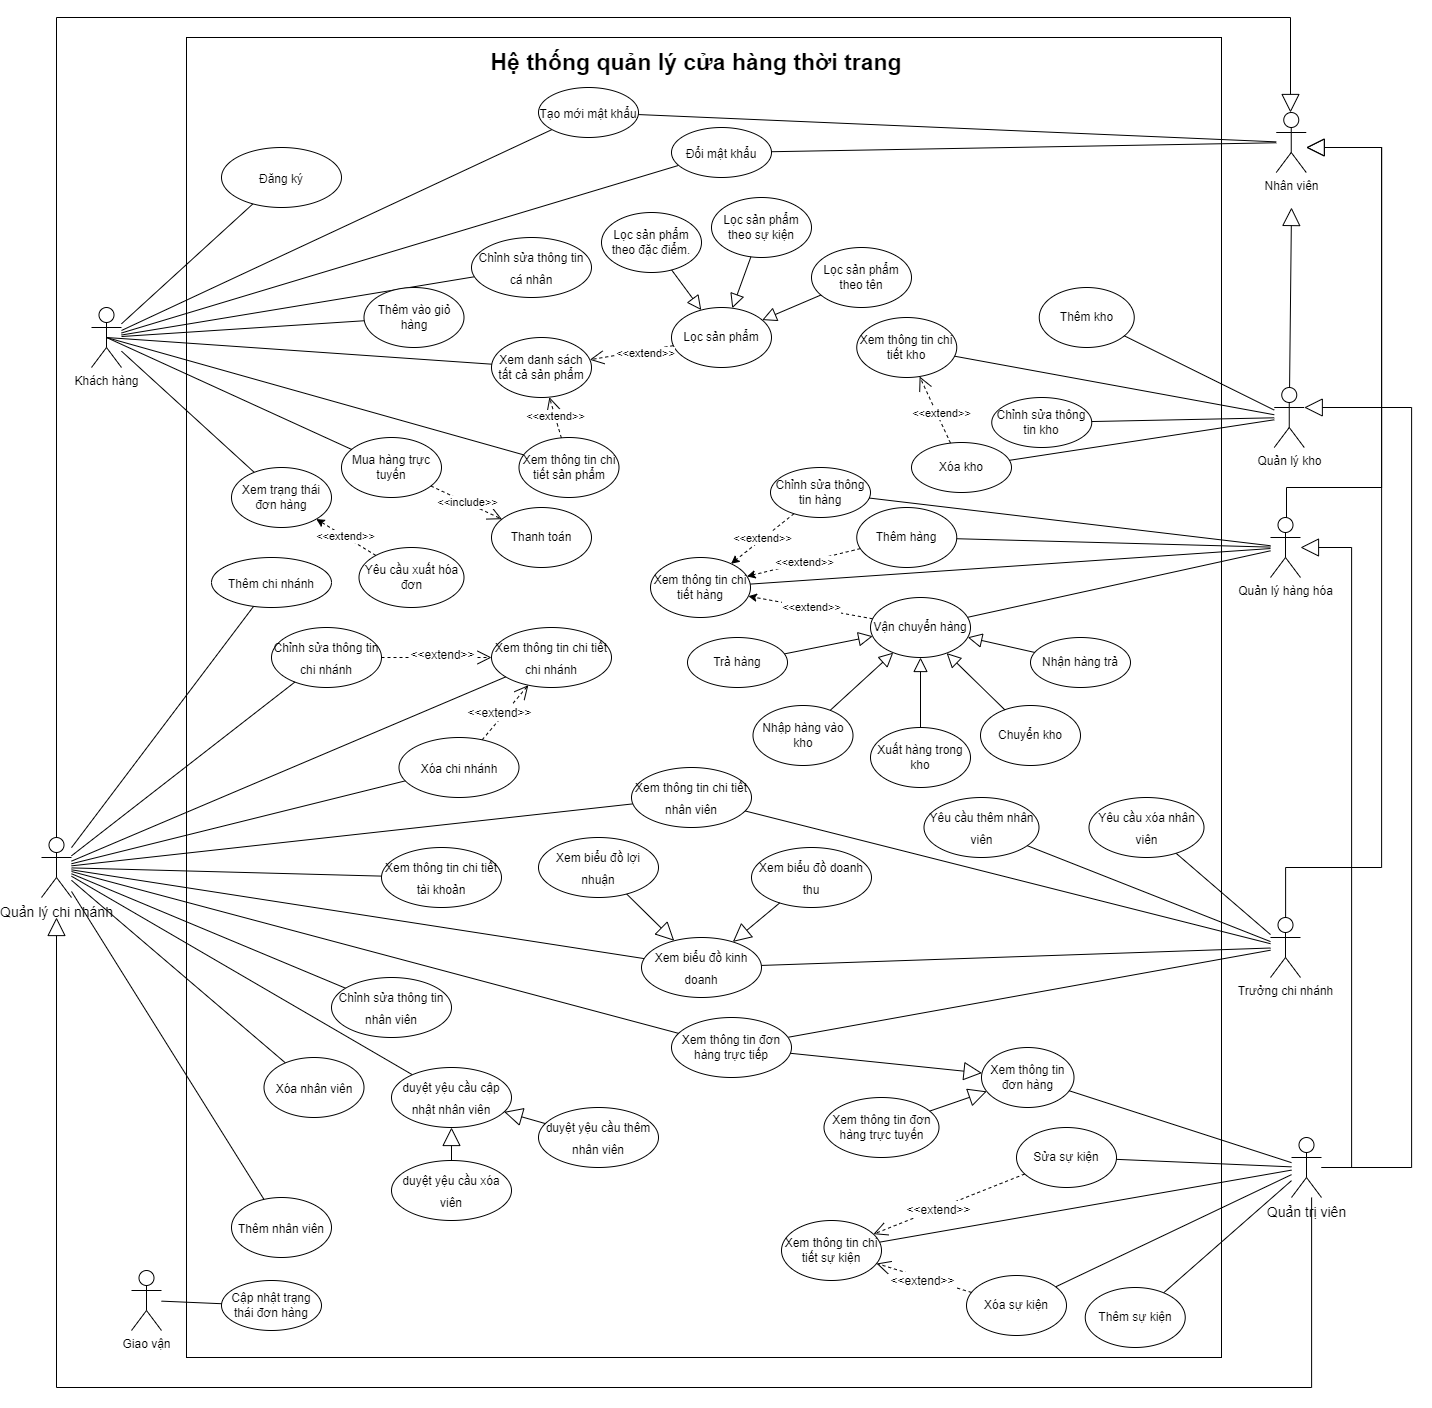
\includegraphics[width=16.5cm]{img/UseCase/UseCase-full.drawio.png}
    \newline
    \caption{Use case Hệ thống quản lý cửa hàng thời trang}
\end{figure}
\textbf{Lưu ý:} Các Usecase không yêu cầu đăng nhập:
\begin{itemize}
    \item Đăng ký
    \item Tạo mới mật khẩu
    \item Xem danh sách sản phẩm
    \item Lọc sản phẩm
    \item Điểm danh
\end{itemize}
\newpage


\subsection{Đặt hàng trực tuyến}

\begin{figure}[!htp]
    \centering
    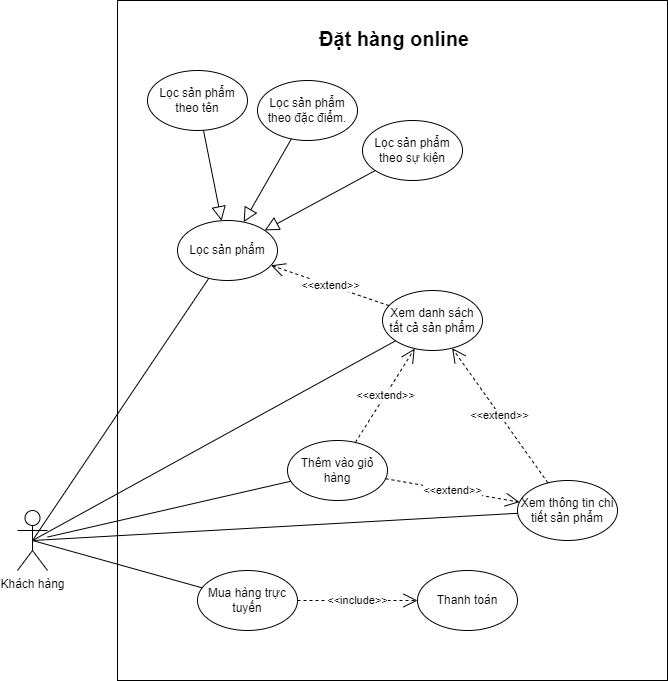
\includegraphics[width=12cm]{img/UseCase/UseCase-Đặt hàng.drawio.png}
    \newline
    \caption{Use case đặt hàng trực tuyến}
\end{figure}
\subsubsection{Xem danh sách sản phẩm}
\begin{center}
    {
        \setlength\extrarowheight{6pt}
        \begin{longtable}{| p{.20\textwidth} | p{.80\textwidth} |}
            \hline
            \textbf{Use-case name}
             &
            Xem danh sách sản phẩm
            \\
            \hline
            \textbf{Actor}
             &
            Người dùng
            \\
            \hline
            \textbf{Description}
             &
            Cho phép người dùng có thể xem danh sách các sản phẩm của cửa hàng.
            \\
            \hline
            \textbf{Preconditions}
             &
            Người dùng đã truy cập vào trang chủ của hệ thống.
            \\
            \hline
            \textbf{Postconditions}
             &
            Người dùng xem được danh sách các sản phẩm thời trang của cửa hàng.
            \\
            \hline
            \textbf{Trigger}
             &
            Không.
            \\
            \hline
            \textbf{Normal flow}
             &
            1. Hệ thống hiển thị các sản phẩm theo mặc định.

            2. Người dùng chọn mục tất cả sản phẩm.

            3. Hệ thống hiển thị toàn bộ sản phẩm có bán trong cửa hàng.

            4. Người dùng lướt trang web để duyệt tất cả các sản phẩm của cửa hàng.
            \\
            \hline
            \textbf{Alternative flow}
             &
            2.1 Người dùng lướt trang chủ để xem các sản phẩm nổi bật mặc định của trang web.
            \\
            %%%%%%%%%%%%%%%%
            \hline
            \textbf{Exceptions}
             &
            Không
            %%%%%%%%%%%%%%%%%%%%
            \\
            \hline
            \caption{Đặc tả use-case \textbf{xem danh sách sản phẩm}}
        \end{longtable}
    }

\end{center}


\subsubsection{Lọc sản phẩm theo từ khóa}
\begin{center}
    {
        \setlength\extrarowheight{6pt}
        \begin{longtable}{| p{.20\textwidth} | p{.80\textwidth} |}
            \hline
            \textbf{Use-case name}
             &
            Lọc danh sách sản phẩm theo từ khóa
            \\
            \hline
            \textbf{Actor}
             &
            Người dùng
            \\
            \hline
            \textbf{Description}
             &
            Cho phép người dùng có thể xem danh sách các sản phẩm của cửa hàng có chứa tên mà người dùng mong muốn.
            \\
            \hline
            \textbf{Preconditions}
             &
            Người dùng đã truy cập vào trang chủ của nhà hàng.
            \\
            \hline
            \textbf{Postconditions}
             &
            Người dùng xem được danh sách các sản phẩm  của cửa hàng có tên chứa từ khóa mà người dùng muốn xem.
            \\
            \hline
            \textbf{Trigger}
             &
            Không.
            \\
            \hline
            \textbf{Normal flow}
             &
            1. Hệ thống hiển thị các sản phẩm theo mặc định.

            2. Người dùng nhập từ khóa của sản phẩm muốn tìm.

            3. Hệ thống hiển thị toàn bộ sản phẩm mà tên có từ khóa mà khách hàng tìm kiếm.

            4. Người dùng xem kết quả danh sách sản phẩm tìm kiếm của hệ thống.
            \\
            \hline
            \textbf{Alternative flow}
             &
            Không
            %%%%%%%%%%%%%%%%
            \\
            \hline
            \textbf{Exceptions}
             &
            Không
            %%%%%%%%%%%%%%%%%%%%
            \\
            \hline
            \caption{Đặc tả use-case \textbf{lọc sản phẩm theo từ khóa}}
        \end{longtable}
    }
\end{center}


\subsubsection{Lọc sản phẩm theo sự kiện }
\begin{center}
    {
        \setlength\extrarowheight{6pt}
        \begin{longtable}{| p{.20\textwidth} | p{.80\textwidth} |}
            \hline
            \textbf{Use-case name}
             &
            Lọc danh sách sản phẩm theo sự kiện
            \\
            \hline
            \textbf{Actor}
             &
            Người dùng
            \\
            \hline
            \textbf{Description}
             &
            Cho phép người dùng có thể xem các sản phẩm của cửa hàng đang trong danh sách thuộc sự kiện mà người dùng muốn xem.
            \\
            \hline
            \textbf{Preconditions}
             &
            Người dùng đã truy cập vào trang chủ của nhà hàng.
            \\
            \hline
            \textbf{Postconditions}
             &
            Người dùng xem được các sản phẩm của cửa hàng đang trong danh sách thuộc sự kiện mà người dùng muốn xem.
            \\
            \hline
            \textbf{Trigger}
             &
            Không
            \\
            \hline
            \textbf{Normal flow}
             &
            1. Hệ thống hiển thị các sự kiện trong trang mặc định.

            2. Người dùng chọn sự kiện muốn xem.

            3. Hệ thống hiển thị toàn bộ sản phẩm mà có trong danh sách thuộc sự kiện người dùng chọn.

            4. Người dùng xem kết quả danh sách sản phẩm sau khi lọc.
            \\
            \hline
            \textbf{Alternative flow}
             &
            Không
            %%%%%%%%%%%%%%%%
            \\
            \hline
            \textbf{Exceptions}
             &
            Không
            %%%%%%%%%%%%%%%%%%%%
            \\
            \hline
            \caption{Đặc tả use-case \textbf{lọc sản phẩm theo sự kiện}}
        \end{longtable}
    }
\end{center}


\subsubsection{Lọc sản phẩm theo đặc điểm }
\begin{center}
    {
        \setlength\extrarowheight{6pt}
        \begin{longtable}{| p{.20\textwidth} | p{.80\textwidth} |}
            \hline
            \textbf{Use-case name}
             &
            Lọc danh sách sản phẩm theo đặc điểm
            \\
            \hline
            \textbf{Actor}
             &
            Người dùng
            \\
            \hline
            \textbf{Description}
             &
            Cho phép người dùng có thể xem các sản phẩm của cửa hàng có các đặc điểm của các thể loại mà người dùng chọn.
            \\
            \hline
            \textbf{Preconditions}
             &
            Người dùng đã vào trang tất cả sản phẩm của nhà hàng.
            \\
            \hline
            \textbf{Postconditions}
             &
            Người dùng xem được các sản phẩm của cửa hàng có các đặc điểm của thể loại mà người dùng muốn xem.
            \\
            \hline
            \textbf{Trigger}
             &
            Người dùng chọn "Tất cả sản phẩm".
            \\
            \hline
            \begin{flushleft}
                \textbf{Normal flow}
            \end{flushleft}
             &
            1. Người dùng chọn đặc điểm của các trường muốn lọc (Các trường này theo bao gồm giá, thương hiệu, gender, size, màu sắc, nhóm sản phẩm).

            2. Hệ thống hiển thị toàn bộ sản phẩm mà có các đặc điểm mà người dùng chọn.

            3. Người dùng xem kết quả danh sách sản phẩm sau khi lọc.
            \\
            \hline
            \textbf{Alternative flow}
             &
            Không
            %%%%%%%%%%%%%%%%
            \\
            \hline
            \textbf{Exceptions}
             &
            Không
            %%%%%%%%%%%%%%%%%%%%
            \\
            \hline
            \caption{Đặc tả use-case \textbf{lọc sản phẩm theo đặc điểm}}
        \end{longtable}
    }

\end{center}


\subsubsection{Xem thông tin chi tiết sản phẩm }
{
    \setlength\extrarowheight{6pt}
    \begin{longtable}{| p{.20\textwidth} | p{.80\textwidth} |}
        \hline
        \textbf{Use-case name}
         &
        Xem thông tin chi tiết sản phẩm
        \\
        \hline
        \textbf{Actor}
         &
        Người dùng
        \\
        \hline
        \textbf{Description}
         &
        Cho phép người dùng có thể xem thông tin chi tiết của sản phẩm.
        \\
        \hline
        \textbf{Preconditions}
         &
        Người dùng đang xem danh sách các sản phẩm.
        \\
        \hline
        \textbf{Postconditions}
         &
        Người dùng xem được thông tin chi tiết của sản phẩm mà người dùng muốn xem.
        \\
        \hline
        \begin{flushleft}
            \textbf{Normal flow}
        \end{flushleft}
         &
        1. Người dùng chọn vào sản phẩm muốn xem trong danh sách các sản phẩm đang xem.

        2. Hệ thống hiển thị thông tin chi tiết của sản phẩm.

        3. Người dùng xem thông tin chi tiết của sản phẩm.
        \\
        \hline
        \textbf{Alternative flow}
         &
        1.1. Người dùng xem danh sách sản phẩm trong giỏ hàng.

        1.2. Người dùng xem danh sách sản phẩm trong lịch sử mua hàng.
        %%%%%%%%%%%%%%%%
        \\
        \hline
        \textbf{Exceptions}
         &
        Không
        %%%%%%%%%%%%%%%%%%%%
        \\
        \hline
        \caption{Đặc tả use-case \textbf{xem thông tin chi tiết sản phẩm}}
    \end{longtable}
}


\subsubsection{ Thêm sản phẩm vào giỏ hàng}
{
    \setlength\extrarowheight{6pt}
    \begin{longtable}{| p{.20\textwidth} | p{.80\textwidth} |}
        \hline
        \textbf{Use-case name}
         &
        Thêm sản phẩm vào giỏ hàng
        \\
        \hline
        \textbf{Actor}
         &
        Người dùng
        \\
        \hline
        \textbf{Description}
         &
        Cho phép người dùng thêm sản phẩm vào giỏ hàng của tài khoản của họ.
        \\
        \hline
        \textbf{Preconditions}
         &
        Người dùng đã đăng nhập vào hệ thống.
        \\
        \hline
        \textbf{Postconditions}
         &
        Người dùng thêm sản phẩm vào giỏ hàng của tài khoản của họ.
        \\
        \hline
        \textbf{Triggers}
         &
        Không.
        \\
        \hline
        \begin{flushleft}
            \textbf{Normal flow}
        \end{flushleft}
         &
        1. Người dùng chọn vào xem danh sách các sản phẩm.

        2. Hệ thống hiển thị danh sách các sản phẩm của người dùng chọn

        3. Người dùng chọn xem thông tin chi tiết sản phẩm.

        4. Hệ thống hiển thị thông tin chi tiết sản phẩm.

        5. Người dùng chọn các thông tin sản phẩm theo ý muốn (Thông tin bao gồm size, màu... tùy thuộc loại sản phẩm).

        6. Hệ thống thực hiện yêu cầu và hiển thị kết quả.

        7. Người dùng nhận kết quả thêm vào giỏ hàng thành công.
        \\
        \hline
        \begin{flushleft}
            \textbf{Alternative flow}
        \end{flushleft}
         &
        1.1 Người dùng thêm vào giỏ từ lịch sử mua hàng.
        \begin{quote}
            1.1.1. Người dùng chọn xem đơn hàng đã mua.

            1.1.2. Hệ thống hiển thị danh sách các đơn hàng đã mua của người dùng.

            1.1.3. Người dùng chọn thêm lại vào giỏ hàng.

            1.1.4. Hệ thống thực hiện yêu cầu và hiển thị kết quả.

            1.1.5. Người dùng nhận kết quả thêm vào giỏ hàng thành công.

        \end{quote}
        3.1 Người dùng chọn thêm nhanh vào giỏ hàng.
        \begin{quote}
            3.1.1 Hệ thống thêm sản phẩm vào giỏ hàng của khách hàng với các thông tin mặc định của hệ thống và thông báo kết quả.

            3.1.2. Đến bước 7.
        \end{quote}
        %%%%%%%%%%%%%%%%
        \\
        \hline
        \begin{flushleft}
            \textbf{Exceptions}
        \end{flushleft}
         &
        7.1.Thêm vào giỏ hàng thất bại.
        \begin{quote}
            7.1.1 Quay lại bước 5.
        \end{quote}
        %%%%%%%%%%%%%%%%%%%%
        \\
        \hline
        \caption{Đặc tả use-case \textbf{thêm sản phẩm vào giỏ hàng}}
    \end{longtable}
}


\subsubsection{Mua hàng trực tuyến }
{
    \setlength\extrarowheight{6pt}
    \begin{longtable}{| p{.20\textwidth} | p{.80\textwidth} |}
        \hline
        \textbf{Use-case name}
         &
        Mua hàng trực tuyến
        \\
        \hline
        \textbf{Actor}
         &
        Người dùng
        \\
        \hline
        \textbf{Description}
         &
        Cho phép người dùng đặt hàng những sản phẩm mà họ muốn.
        \\
        \hline
        \textbf{Preconditions}
         &
        Người dùng đã đăng nhập vào hệ thống.
        \\
        \hline
        \textbf{Postconditions}
         &
        Người dùng đặt hàng thành công các sản phẩm mà họ muốn.
        \\
        \hline
        \begin{flushleft}
            \textbf{Normal flow}
        \end{flushleft}
         &
        1. Người dùng chọn giỏ hàng.

        2. Hệ thống hiển thị danh sách thông tin các sản phẩm trong giỏ hàng.

        3. Người dùng chỉnh sửa các thông tin sản phẩm theo ý muốn (Thông tin bao gồm size, màu... tùy thuộc loại sản phẩm).

        4. Hệ thống tính toán và hiển thị tổng giá tiền.

        5. Người dùng chọn đặt hàng.

        6. Hệ thống hiển thị màn hình danh sách thông tin sản phẩm mà người dùng đã chọn cùng giá tiền.

        7. Người dùng chọn và nhập địa chỉ giao hàng.

        8. Hệ thống nhận thông tin giao hàng và tính toán sau đó hiển thị kết quả lên màn hình.

        % 9. Người dùng nhập mã giảm giá.

        % 10. Hệ thống tính toán giá trị mã giảm giá và hiển thị giá cuối cùng cho người dùng.

        9. Người dùng chọn thanh toán và thực hiện thanh toán tùy chọn.

        10. Hệ thống thông báo kết quả đơn hàng hoàn tất cho người dùng.
        \\
        \hline
        \begin{flushleft}
            \textbf{Alternative flow}
        \end{flushleft}
         &
        3.1. Chưa có sản phẩm trong giỏ hàng.
        \begin{quote}
            3.1.1. Người dùng thực hiện tìm kiếm sản phẩm mình muốn và thêm vào giỏ hàng.

            3.1.2. Quay lại bước 1.
        \end{quote}
        5.1 Người dùng không muốn tiếp tục đặt hàng.
        \begin{quote}
            5.1.1. Người dùng chọn logo của trang web trên header.
            5.1.2. Hệ thống chuyển hướng về lại trang mặc định.
        \end{quote}
        % 9.1. Người dùng không muốn nhập mã giảm giá.
        % \begin{quote}
        %     9.1.1. Đến bước 11.
        % \end{quote}
        %%%%%%%%%%%%%%%%
        \\
        \hline
        \begin{flushleft}
            \textbf{Exceptions}
        \end{flushleft}
         &
        % 8.2. Địa chỉ khách hàng không được đơn vị vận chuyển hỗ trợ.
        % \begin{quote}
        %     8.2.1. Hệ thống thông báo cho người dùng và yêu cầu chỉnh sửa địa chỉ giao hàng.
        %     8.2.2. Quay lại bước 7.
        % \end{quote}
        % 10.1. Khách hàng thực hiện thanh toán thất bại khi chọn thanh toán online.
        % \begin{quote}
        %     10.1.1. Hệ thống thông báo cho người dùng đặt hàng thất bại và thực hiện lại thanh toán.
        %     10.1.2. Quay lại bước 9.
        % \end{quote}
        %%%%%%%%%%%%%%%%%%%%
        \\
        \hline
        \caption{Đặc tả use-case \textbf{mua hàng trực tuyến}}
    \end{longtable}
}
\subsubsection{Thanh toán}
{
    \setlength\extrarowheight{6pt}
    \begin{longtable}{| p{.20\textwidth} | p{.80\textwidth} |}
        \hline
        \textbf{Use-case name}
         &
        Thanh toán
        \\
        \hline
        \textbf{Actor}
         &
        Người dùng
        \\
        \hline
        \textbf{Description}
         &
        Cho phép người dùng có thể thực hiện thanh toán để hoàn tất đơn hàng.
        \\
        \hline
        \textbf{Preconditions}
         &
        Người dùng tiến hành đặt hàng.
        \\
        \hline
        \textbf{Postconditions}
         &
        Người dùng thanh toán đơn hàng thành công.
        \\
        \hline
        \textbf{Trigger}
         &
        Người dùng chọn "Thanh toán".
        \\
        \hline
        \begin{flushleft}
            \textbf{Normal flow}
        \end{flushleft}
         &
        1. Hệ thống hiển thị lựa chọn thanh toán cho khách hàng gồm "Thanh toán online" và "Thanh toán khi nhận hàng".

        2. Người dùng chọn "Thanh toán online".

        3. Hệ thống hiển thị các dịch vụ hỗ trợ thanh toán trực tuyến.

        4. Người dùng chọn dịch vụ thanh toán trực tuyến mà người dùng muốn.

        5. Hệ thống tổng hợp dữ liệu gửi cho bên dịch vụ thứ ba mà người dùng chọn sau đó liên kết hiển thị cho người dùng thực hiện thanh toán.

        6. Người dùng thực hiện thanh toán thông qua dịch vụ của bên thứ ba.

        7. Hệ thống bên thứ ba trả về kết quả thanh toán thành công cho hệ thống và hệ thống thực thông báo kết quả thanh toán cho người dùng.

        8. Người dùng xem kết quả giao dịch thanh toán.
        \\
        \hline
        \begin{flushleft}
            \textbf{Alternative flow}
        \end{flushleft}
         &
        2.1. Người dùng chọn "Thanh toán khi nhận hàng".
        \begin{quote}
            2.1.1. Hệ thống hiển thị xác nhận, ghi nợ cho vận chuyển và thông báo kết quả thành công.

            2.1.2. Người dùng xem kết quả.
        \end{quote}
        %%%%%%%%%%%%%%%%
        \\
        \hline
        \begin{flushleft}
            \textbf{Exceptions}
        \end{flushleft}
         &
        7.1. Thanh toán thất bại.
        \begin{quote}
            7.1.1. Hệ thống thông báo thanh toán thất bại.

            7.1.2. Quay lại bước 8.
        \end{quote}
        2.1.1.1. Xác nhận đơn hàng thất bại.
        \begin{quote}
            2.1.1.1.1 Hệ thống thông báo kết quả tạo đơn thanh toán khi nhận hàng thất bại.

            2.1.1.1.2 Quay lại bước 2.1.2.
        \end{quote}
        %%%%%%%%%%%%%%%%%%%%
        \\
        \hline
        \caption{Đặc tả use-case \textbf{Thanh toán}}
    \end{longtable}
}


\subsection{Quản lý sự kiện}
\newpage
\begin{figure}[!htp]
    \centering
    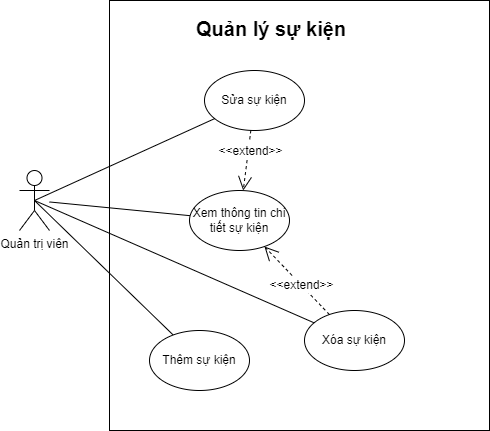
\includegraphics[width=8cm]{img/UseCase/UseCase-Quản lý sự kiện.drawio.png}
    \newline
    \caption{Use case quản lý sự kiện}
\end{figure}
\subsubsection{Xem thông tin chi tiết sự kiện}
{
    \setlength\extrarowheight{6pt}
    \begin{longtable}{| p{.20\textwidth} | p{.80\textwidth} |}
        \hline
        \textbf{Use-case name}
         &
        Xem thông tin chi tiết sự kiện.
        \\
        \hline
        \textbf{Actor}
         &
        Quản trị viên
        \\
        \hline
        \textbf{Description}
         &
        Cho phép quản trị viên xem  thông tin chi tiết sự kiện trong hệ thống.
        \\
        \hline
        \textbf{Preconditions}
         &
        Quản trị viên đã đăng nhập thành công vào hệ thống.
        \\
        \hline
        \textbf{Postconditions}
         &
        Quản trị viên xem được được thông tin chi tiết của sự kiện mà họ muốn.
        \\
        \hline
        \textbf{Trigger}
         &
        Quản trị viên chọn mục "sự kiện".
        \\
        \hline
        \begin{flushleft}
            \textbf{Normal flow}
        \end{flushleft}
         &
        1. Toàn bộ sự kiện được hiển thị lên trình duyệt.

        2.  Quản trị viên chọn sự kiện muốn xem thông tin chi tiết và nhấp chuột vào sự kiện đó.

        3.  Hệ thống hiển thị thông tin chi tiết của sự kiện.

        4. Người dùng xem thông tin chi tiết của sự kiện.
        \\
        \hline
        \textbf{Alternative flow}
         &
        Không.
        %%%%%%%%%%%%%%%%
        \\
        \hline
        \textbf{Exceptions}
         &
        Không.
        %%%%%%%%%%%%%%%%%%%%
        \\
        \hline
        \caption{Đặc tả use-case \textbf{xem thông tin chi tiết sự kiện}}
    \end{longtable}
}
\subsubsection{Thêm sự kiện cho hệ thống bán hàng online.}
{
    \setlength\extrarowheight{6pt}
    \begin{longtable}{| p{.20\textwidth} | p{.80\textwidth} |}
        \hline
        \textbf{Use-case name}
         &
        Thêm sự kiện cho hệ thống bán hàng online
        \\
        \hline
        \textbf{Actor}
         &
        Quản trị viên
        \\
        \hline
        \textbf{Description}
         &
        Cho phép quản trị viên có thể thêm sự kiện mới cho hệ thống bán hàng online.
        \\
        \hline
        \textbf{Preconditions}
         &
        Quản trị viên đã đăng nhập thành công vào hệ thống.
        \\
        \hline
        \textbf{Postconditions}
         &
        Quản trị viên tạo mới được sự kiện mà họ muốn.
        \\
        \hline
        \textbf{Trigger}
         &
        Quản trị viên chọn mục "sự kiện".
        \\
        \hline
        \begin{flushleft}
            \textbf{Normal flow}
        \end{flushleft}
         &
        1. Toàn bộ sự kiện được hiển thị lên trình duyệt.

        2. Quản trị viên chọn nút thêm sự kiện.

        3. Hệ thống hiển thị màn hình form để tạo sự kiện mới.

        4. Quản trị viên nhập các thông tin cần thiết mà hệ thống yêu cầu và chọn icon "Thêm sự kiện".

        5. Hệ thống cập nhật thêm sự kiện mới vào database.
        \\
        \hline
        \begin{flushleft}
            \textbf{Alternative flow}
        \end{flushleft}
         &
        4.1. Người dùng không muốn tiếp tục nữa.
        \begin{quote}
            4.1.1. Người dùng chọn "Hủy".

            4.1.2. Hệ thống tắt màn hình popup.
        \end{quote}
        %%%%%%%%%%%%%%%%
        \\
        \hline
        \begin{flushleft}
            \textbf{Exceptions}
        \end{flushleft}
         &
        Không
        %%%%%%%%%%%%%%%%%%%%
        \\
        \hline
        \caption{Đặc tả use-case \textbf{thêm sự kiện cho hệ thống bán hàng online}}
    \end{longtable}
}

\subsubsection{Chỉnh sửa sự kiện}
{
    \setlength\extrarowheight{6pt}
    \begin{longtable}{| p{.20\textwidth} | p{.80\textwidth} |}
        \hline
        \textbf{Use-case name}
         &
        Chỉnh sửa thông tin sự kiện
        \\
        \hline
        \textbf{Actor}
         &
        Quản trị viên
        \\
        \hline
        \textbf{Description}
         &
        Cho phép quản trị viên có thể chỉnh sửa thông tin sự kiện mới cho hệ thống bán hàng online.
        \\
        \hline
        \textbf{Preconditions}
         &
        Quản trị viên đã đăng nhập thành công vào hệ thống.
        \\
        \hline
        \textbf{Postconditions}
         &
        Quản trị viên chỉnh sửa được sự kiện mà họ muốn.
        \\
        \hline
        \textbf{Trigger}
         &
        Quản trị viên chọn mục "sự kiện".
        \\
        \hline
        \begin{flushleft}
            \textbf{Normal flow}
        \end{flushleft}
         &
        1.Toàn bộ sự kiện được hiển thị lên trình duyệt.

        2. Quản trị viên chọn sự kiện muốn chỉnh sửa và nhấn vào nút "chỉnh sửa".

        3. Hệ thống hiển thị màn hình các thông tin của sự kiện.

        4. Quản trị viên chỉnh sửa các thông tin mà họ muốn sau đó nhấn nút "Lưu".

        5. Hệ thống thông báo kết quả cập nhật thêm sự kiện mới vào database.
        \\
        \hline
        \begin{flushleft}
            \textbf{Alternative flow}
        \end{flushleft}
         &
        4.1. Người dùng không muốn tiếp tục nữa.
        \begin{quote}
            4.1.1. Người dùng chọn "Hủy".

            4.1.2. Hệ thống tắt màn hình popup.
        \end{quote}
        %%%%%%%%%%%%%%%%
        \\
        \hline
        \begin{flushleft}
            \textbf{Exceptions}
        \end{flushleft}
         &
        5.1. Thông tin thay đổi không hợp lệ
        \begin{quote}
            5.1.1. Hệ thống thông báo chỉnh sửa sự kiện thất bại

            5.1.2. Trở về bước 4.
        \end{quote}
        %%%%%%%%%%%%%%%%%%%%
        \\
        \hline
        \caption{Đặc tả use-case \textbf{chỉnh sửa thông tin sự kiện}}
    \end{longtable}
}

\subsection{Quản lý chi nhánh}
\begin{figure}[!htp]
    \centering
    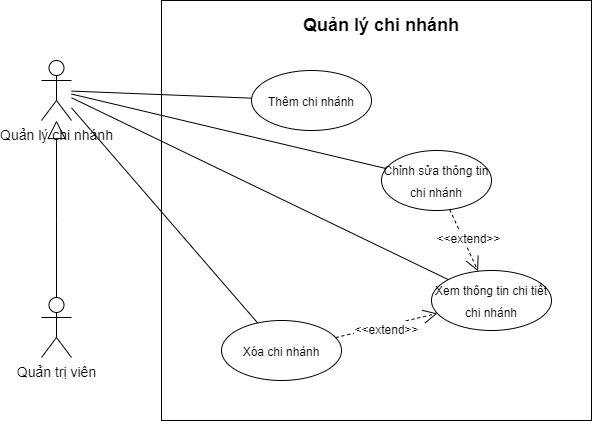
\includegraphics[width=9cm]{img/UseCase/UseCase-Quản lý chi nhánh.drawio.png}
    \newline
    \caption{Use case quản lý chi nhánh}
\end{figure}
\subsubsection{Thêm chi nhánh}
{
    \setlength\extrarowheight{6pt}
    \begin{longtable}{| p{.20\textwidth} | p{.80\textwidth} |}
        \hline
        \textbf{Use-case name}
         &
        Thêm chi nhánh
        \\
        %%%%%%%%%%%%%%%%
        \hline
        \textbf{Actor}
         &
        Quản lý chi nhánh
        \\
        %%%%%%%%%%%%%%%%
        \hline
        \textbf{Description}
         &
        Quản lý chi nhánh có thể thêm chi nhánh mới
        \\
        %%%%%%%%%%%%%%%%
        \hline
        \textbf{Preconditions}
         &
        Quản lý chi nhánh đã đăng nhập
        \\
        %%%%%%%%%%%%%%%%
        \hline
        \textbf{Postconditions}
         &
        Chi nhánh mới được cập nhật
        \\
        %%%%%%%%%%%%%%%%
        \hline
        \textbf{Trigger}
         &
        Quản lý chi nhánh chọn vào quản lý chi nhánh
        \\
        %%%%%%%%%%%%%%%%
        \hline
        \begin{flushleft}
            \textbf{Normal flow}
        \end{flushleft}
         &
        1. Hệ thống hiển thị danh sách chi nhánh

        2. Quản lý chi nhánh chọn thêm mới

        3. Hệ thống hiển thị biểu mẫu nhập thông tin

        4. Quản trị viên nhập thông tin chi nhánh mới

        5. Quản trị viên nhập chọn xác nhận

        6. Hệ thống cập nhật chi nhánh mới
        \\
        %%%%%%%%%%%%%%%%
        \hline
        \begin{flushleft}
            \textbf{Alternative flow}
        \end{flushleft}
         &
        5.1. Quản trị viên nhập chọn hủy
        \begin{quote}
            5.1.1. Kết thúc
        \end{quote}
        \\
        %%%%%%%%%%%%%%%%
        \hline
        \begin{flushleft}
            \textbf{Exceptions}
        \end{flushleft}
         &
        Không
        \\
        \hline
        %%%%%%%%%%%%%%%%
        \caption{Đặc tả use-case \textbf{thêm chi nhánh}}
    \end{longtable}
}
\subsubsection{Chỉnh sửa thông tin chi nhánh}
{
    \setlength\extrarowheight{6pt}
    \begin{longtable}{| p{.20\textwidth} | p{.80\textwidth} |}
        \hline
        \textbf{Use-case name}
         &
        Chỉnh sửa tin chi nhánh
        \\
        %%%%%%%%%%%%%%%%
        \hline
        \textbf{Actor}
         &
        Quản lý chi nhánh
        \\
        %%%%%%%%%%%%%%%%
        \hline
        \textbf{Description}
         &
        Quản lý chi nhánh có thể chỉnh sửa thông tin chi nhánh
        \\
        %%%%%%%%%%%%%%%%
        \hline
        \textbf{Preconditions}
         &
        Quản lý chi nhánh đã đăng nhập
        \\
        %%%%%%%%%%%%%%%%
        \hline
        \textbf{Postconditions}
         &
        Thông tin chi nhánh được cập nhật
        \\
        %%%%%%%%%%%%%%%%
        \hline
        \textbf{Trigger}
         &
        Quản lý chi nhánh chọn vào quản lý chi nhánh
        \\
        %%%%%%%%%%%%%%%%
        \hline
        \begin{flushleft}
            \textbf{Normal flow}
        \end{flushleft}
         &
        1. Hệ thống hiển thị danh sách chi nhánh

        2. Quản lý chi nhánh tìm kiếm chi nhánh và chọn chỉnh sửa

        3. Hệ thống hiển thị biểu mẫu nhập thông tin

        4. Quản lý chi nhánh chỉnh sửa thông tin chi nhánh

        5. Quản lý chi nhánh nhập chọn xác nhận

        6. Hệ thống cập nhật thông tin  chi nhánh
        \\
        %%%%%%%%%%%%%%%%
        \hline
        \begin{flushleft}
            \textbf{Alternative flow}
        \end{flushleft}
         &
        5.1. Quản lý chi nhánh chọn hủy
        \begin{quote}
            5.1.1. Kết thúc
        \end{quote}
        \\
        %%%%%%%%%%%%%%%%
        \hline
        \begin{flushleft}
            \textbf{Exceptions}
        \end{flushleft}
         &
        6.1. Tên chi nhánh bị trùng
        \begin{quote}
            6.1.1. Quay về bước 3
        \end{quote}
        \\
        \hline
        %%%%%%%%%%%%%%%%
        \caption{Đặc tả use-case \textbf{chỉnh sửa chi nhánh}}
    \end{longtable}
}

\subsubsection{Xem thông tin chi tiết chi nhánh}
{
    \setlength\extrarowheight{6pt}
    \begin{longtable}{| p{.20\textwidth} | p{.80\textwidth} |}
        \hline
        \textbf{Use-case name}
         &
        Xem thông tin chi tiết chi nhánh
        \\
        %%%%%%%%%%%%%%%%
        \hline
        \textbf{Actor}
         &
        Quản lý chi nhánh
        \\
        %%%%%%%%%%%%%%%%
        \hline
        \textbf{Description}
         &
        Quản lý chi nhánh có thể xem thông tin chi nhánh
        \\
        %%%%%%%%%%%%%%%%
        \hline
        \textbf{Preconditions}
         &
        Quản lý chi nhánh đã đăng nhập
        \\
        %%%%%%%%%%%%%%%%
        \hline
        \textbf{Postconditions}
         &
        Nhận được thông tin chi nhánh
        \\
        %%%%%%%%%%%%%%%%
        \hline
        \textbf{Trigger}
         &
        Quản lý chi nhánh truy cập quản lý chi nhánh
        \\
        %%%%%%%%%%%%%%%%
        \hline
        \begin{flushleft}
            \textbf{Normal flow}
        \end{flushleft}
         &
        1. Hệ thống hiển thị danh sách các chi nhánh

        2. Quản lý chi nhánh tìm kiếm và chọn chi nhánh muốn xem

        3. Hệ thống hiển thị thông tin chi nhánh đã chọn
        \\
        %%%%%%%%%%%%%%%%
        \hline
        \textbf{Alternative flow}
         &
        Không
        \\
        %%%%%%%%%%%%%%%%
        \hline
        \textbf{Exceptions}
         &
        Không
        \\
        \hline
        %%%%%%%%%%%%%%%%
        \caption{Đặc tả use-case \textbf{xem thông tin chi tiết chi nhánh}}
    \end{longtable}
}
\subsubsection{Xóa chi nhánh}
{
    \setlength\extrarowheight{6pt}
    \begin{longtable}{| p{.20\textwidth} | p{.80\textwidth} |}
        \hline
        \textbf{Use-case name}
         &
        Xóa chi nhánh
        \\
        %%%%%%%%%%%%%%%%
        \hline
        \textbf{Actor}
         &
        Quản lý chi nhánh
        \\
        %%%%%%%%%%%%%%%%
        \hline
        \textbf{Description}
         &
        Quản lý chi nhánh có thể xóa chi nhánh
        \\
        %%%%%%%%%%%%%%%%
        \hline
        \textbf{Preconditions}
         &
        Quản lý chi nhánh đã đăng nhập
        \\
        %%%%%%%%%%%%%%%%
        \hline
        \textbf{Postconditions}
         &
        Chi nhánh bị xóa khỏi hệ thống
        \\
        %%%%%%%%%%%%%%%%
        \hline
        \textbf{Trigger}
         &
        Quản lý chi nhánh chọn quản lý chi nhánh
        \\
        %%%%%%%%%%%%%%%%
        \hline
        \begin{flushleft}
            \textbf{Normal flow}
        \end{flushleft}
         &
        1. Hệ thống hiển thị danh sách chi nhánh

        2. Quản lý chi nhánh tìm và chọn chi nhánh muốn xóa

        3. Hệ thống hiển thị thông tin chi tiết chi nhánh

        4. Quản lý chi nhánh chọn xóa chi nhánh

        5. Hệ thống yêu cầu xác nhận

        6. Quản lý chi nhánh chọn xác nhận

        7. Hệ thống cập nhật thông tin
        \\
        %%%%%%%%%%%%%%%%
        \hline
        \begin{flushleft}
            \textbf{Alternative flow}
        \end{flushleft}
         &
        6.1. Quản trị viên chọn hủy
        \begin{quote}
            6.1.1. Quay lại bước 3
        \end{quote}
        \\
        %%%%%%%%%%%%%%%%
        \hline
        \textbf{Exceptions}
         &
        Không
        \\
        \hline
        %%%%%%%%%%%%%%%%
        \caption{Đặc tả use-case \textbf{xóa chi nhánh}}
    \end{longtable}
}

\subsection{Quản lý hoạt động kinh doanh}
\begin{figure}[!htp]
    \centering
    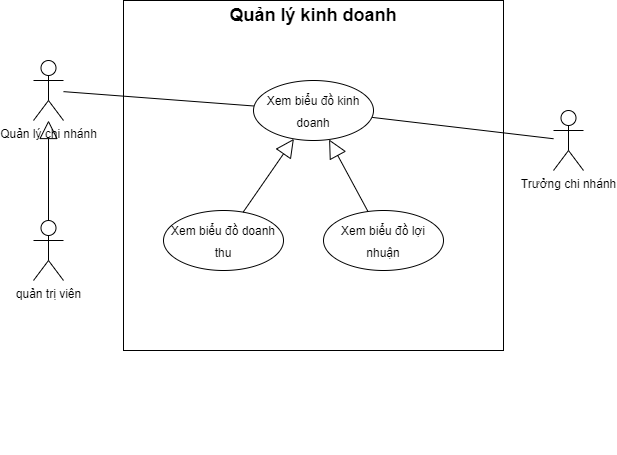
\includegraphics[width=8cm]{img/UseCase/UseCase-Quản lý hoạt động kinh doanh.drawio.png}
    \newline
    \caption{Use case quản lý hoạt động kinh doanh}
\end{figure}
\subsubsection{Xem biểu đồ kinh doanh}
{
    \setlength\extrarowheight{6pt}
    \begin{longtable}{| p{.20\textwidth} | p{.80\textwidth} |}
        \hline
        \textbf{Use-case name}
         &
        Xem biểu đồ kinh doanh
        \\
        %%%%%%%%%%%%%%%%
        \hline
        \textbf{Actor}
         &
        Quản lý chi nhánh, trưởng chi nhánh
        \\
        %%%%%%%%%%%%%%%%
        \hline
        \textbf{Description}
         &
        Quản lý chi nhánh, trưởng chi nhánh có thể xem biểu đồ kinh doanh
        \\
        %%%%%%%%%%%%%%%%
        \hline
        \textbf{Preconditions}
         &
        Quản lý chi nhánh, trưởng chi nhánh đã đăng nhập
        \\
        %%%%%%%%%%%%%%%%
        \hline
        \textbf{Postconditions}
         &
        Nhận được biểu đồ kinh doanh
        \\
        %%%%%%%%%%%%%%%%
        \hline
        \textbf{Trigger}
         &
        Quản lý chi nhánh, trưởng chi nhánh chọn quản lý hoạt động kinh doanh
        \\
        %%%%%%%%%%%%%%%%
        \hline
        \begin{flushleft}
            \textbf{Normal flow}
        \end{flushleft}
         &
        1. Quản lý chi nhánh, trưởng chi nhánh loại hàng muốn thống kê

        2. Quản lý chi nhánh, trưởng chi nhánh chọn khoảng thời gian

        3. Quản lý chi nhánh, trưởng chi nhánh chọn loại biểu đồ

        4. Hệ thống hiển thị biểu đồ
        \\
        %%%%%%%%%%%%%%%%
        \hline
        \textbf{Alternative flow}
         &
        Không
        \\
        %%%%%%%%%%%%%%%%
        \hline
        \textbf{Exceptions}
         &
        Không
        \\
        \hline
        %%%%%%%%%%%%%%%%
        \caption{Đặc tả use-case \textbf{xem biểu đồ kinh doanh}}
    \end{longtable}
}


\subsection{Quản lý nhân viên}
\begin{figure}[!htp]
    \begin{center}
        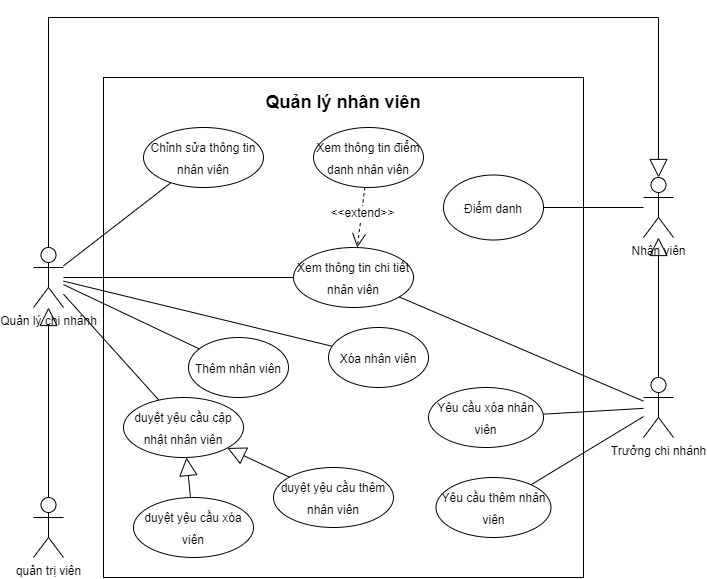
\includegraphics[width=10cm]{img/UseCase/UseCase-Quản lý nhân viên.drawio.png}
    \end{center}
    \caption{Use case quản lý nhân viên}
\end{figure}
\newpage


\subsubsection{Xem thông tin chi tiết nhân viên}
{
    \setlength\extrarowheight{6pt}
    \begin{longtable}{| p{.20\textwidth} | p{.80\textwidth} |}
        \hline
        \textbf{Use-case name}
         &
        Xem thông tin chi tiết nhân viên
        \\
        %%%%%%%%%%%%%%%%%%
        \hline
        \textbf{Actor}
         &
        Quản lý chi nhánh, trưởng chi nhánh
        \\
        %%%%%%%%%%%%%%%%%%
        \hline
        \textbf{Description}
         &
        Quản lý chi nhánh, trưởng chi nhánh có thể xem thông tin chi tiết nhân viên
        \\
        %%%%%%%%%%%%%%%%%%
        \hline
        \textbf{Preconditions}
         &
        Quản lý chi nhánh, trưởng chi nhánh đã đăng nhập
        \\
        %%%%%%%%%%%%%%%%%%
        \hline
        \textbf{Postconditions}
         &
        Nhận được thông tin chi tiết nhân viên
        \\
        %%%%%%%%%%%%%%%%%%
        \hline
        \textbf{Trigger}
         &
        Quản lý chi nhánh, trưởng chi nhánh chọn quản lý nhân viên
        \\
        %%%%%%%%%%%%%%%%%%
        \hline
        \begin{flushleft}
            \textbf{Normal flow}
        \end{flushleft}
         &
        1. Hệ thống hiển thị danh sách nhân viên

        2. Quản lý chi nhánh, trưởng chi nhánh tìm và chọn nhân viên muốn xem

        3. Hệ thống hiển thị thông tin chi tiết nhân viên
        \\
        %%%%%%%%%%%%%%%%%%
        \hline
        \textbf{Alternative flow}
         &
        Không
        \\
        %%%%%%%%%%%%%%%%%%
        \hline
        \textbf{Exceptions}
         &
        Không
        \\
        %%%%%%%%%%%%%%%%%%
        \hline
        \caption{Đặc tả use-case \textbf{xem thông tin chi tiết nhân viên}}
    \end{longtable}
}

\newpage

\subsubsection{Chỉnh sửa thông tin chi tiết nhân viên}
{
    \setlength\extrarowheight{6pt}
    \begin{longtable}{| p{.20\textwidth} | p{.80\textwidth} |}
        \hline
        \textbf{Use-case name}
         &
        Chỉnh sửa thông tin chi tiết nhân viên
        \\
        %%%%%%%%%%%%%%%%%%
        \hline
        \textbf{Actor}
         &
        Quản lý chi nhánh
        \\
        %%%%%%%%%%%%%%%%%%
        \hline
        \textbf{Description}
         &
        Quản lý chi nhánh có thể chỉnh sửa thông tin nhân viên.
        \\
        %%%%%%%%%%%%%%%%%%
        \hline
        \textbf{Preconditions}
         &
        Quản lý chi nhánh đã đăng nhập
        \\
        %%%%%%%%%%%%%%%%%%
        \hline
        \textbf{Postconditions}
         &
        Thông tin nhân viên được cập nhật
        \\
        %%%%%%%%%%%%%%%%%%
        \hline
        \textbf{Trigger}
         &
        Quản lý chi nhánh chọn quản lý nhân viên
        \\
        %%%%%%%%%%%%%%%%%%
        \hline
        \begin{flushleft}
            \textbf{Normal flow}
        \end{flushleft}
         &
        1. Hệ thống hiển thị danh sách  nhân viên

        2. Quản lý chi nhánh tìm và chọn nhân viên cần chỉnh sửa

        3. Hệ thống hiển thị biểu mẫu thông tin nhân viên

        4. Quản lý chỉnh sửa thông tin

        5. Quản lý chọn lưu

        6. Hệ thống cập nhật thông tin
        \\
        %%%%%%%%%%%%%%%%%%
        \hline
        \begin{flushleft}
            \textbf{Alternative flow}
        \end{flushleft}
         &
        5.1. Quản lý chọn hủy
        \begin{quote}
            5.1.1. Quay lại bước 3
        \end{quote}
        \\
        %%%%%%%%%%%%%%%%%%
        \hline
        \textbf{Exceptions}
         &
        Không
        \\
        %%%%%%%%%%%%%%%%%%
        \hline
        \caption{Đặc tả use-case \textbf{chỉnh sửa thông tin nhân viên}}
    \end{longtable}
}

\subsubsection{Thêm nhân viên}
{
    \setlength\extrarowheight{6pt}
    \begin{longtable}{| p{.20\textwidth} | p{.80\textwidth} |}
        \hline
        \textbf{Use-case name}
         &
        Thêm nhân viên
        \\
        %%%%%%%%%%%%%%%%%%
        \hline
        \textbf{Actor}
         &
        Quản lý chi nhánh
        \\
        %%%%%%%%%%%%%%%%%%
        \hline
        \textbf{Description}
         &
        Quản lý chi nhánh có thể thêm nhân viên
        \\
        %%%%%%%%%%%%%%%%%%
        \hline
        \textbf{Preconditions}
         &
        Quản lý chi nhánh đã đăng nhập
        \\
        %%%%%%%%%%%%%%%%%%
        \hline
        \textbf{Postconditions}
         &
        Thông tin nhân viên mới được cập nhật
        \\
        %%%%%%%%%%%%%%%%%%
        \hline
        \textbf{Trigger}
         &
        Quản lý chi nhánh chọn quản lý nhân viên
        \\
        %%%%%%%%%%%%%%%%%%
        \hline
        \begin{flushleft}
            \textbf{Normal flow}
        \end{flushleft}
         &
        1. Hệ thống hiển thị danh sách nhân viên

        2. Quản lý chi nhánh chọn thêm mới

        3. Hệ thống hiển thị biểu mẫu thông tin  nhân viên mới

        4. Quản lý chi nhánh nhập thông tin nhân viên

        5. Quản lý chi nhánh chọn lưu

        6. Hệ thống cập nhật thông tin
        \\
        %%%%%%%%%%%%%%%%%%
        \hline
        \begin{flushleft}
            \textbf{Alternative flow}
        \end{flushleft}
         &
        5.1. Quản lý chọn hủy
        \begin{quote}
            5.1.1. Quay lại bước 3
        \end{quote}
        \\
        %%%%%%%%%%%%%%%%%%
        \hline
        \textbf{Exceptions}
         &
        Không
        \\
        %%%%%%%%%%%%%%%%%%
        \hline
        \caption{Đặc tả use-case \textbf{Thêm nhân viên}}
    \end{longtable}
}

\subsubsection{Xóa nhân viên}
{
    \setlength\extrarowheight{6pt}
    \begin{longtable}{| p{.20\textwidth} | p{.80\textwidth} |}
        \hline
        \textbf{Use-case name}
         &
        Xóa nhân viên
        \\
        %%%%%%%%%%%%%%%%%%
        \hline
        \textbf{Actor}
         &
        Quản lý chi nhánh
        \\
        %%%%%%%%%%%%%%%%%%
        \hline
        \textbf{Description}
         &
        Quản lý chi nhánh có thể xóa nhân viên
        \\
        %%%%%%%%%%%%%%%%%%
        \hline
        \textbf{Preconditions}
         &
        Quản lý chi nhánh đã đăng nhập
        \\
        %%%%%%%%%%%%%%%%%%
        \hline
        \textbf{Postconditions}
         &
        Thông tin nhân viên được xóa
        \\
        %%%%%%%%%%%%%%%%%%
        \hline
        \textbf{Trigger}
         &
        Quản lý chi nhánh chọn quản lý nhân viên
        \\
        %%%%%%%%%%%%%%%%%%
        \hline
        \begin{flushleft}
            \textbf{Normal flow}
        \end{flushleft}
         &
        1. Hệ thống hiển thị danh sách nhân viên

        2. Quản lý chi nhánh tìm và chọn nhân viên muốn xóa

        3. Hệ thống hiển thị thông tin chi tiết nhân viên

        4. Quản lý chi nhánh chọn xóa

        5. Hệ thống yêu cầu xác nhận

        6. Quản lý chi nhánh chọn xác nhận

        7. Hệ thống cập nhật thông tin
        \\
        %%%%%%%%%%%%%%%%%%
        \hline
        \textbf{Alternative flow}
         &
        6.1. Quản lý chọn hủy
        \begin{quote}
            6.1.1. Quay lại bước 3
        \end{quote}
        \\
        %%%%%%%%%%%%%%%%%%
        \hline
        \textbf{Exceptions}
         &
        Không
        \\
        %%%%%%%%%%%%%%%%%%
        \hline
        \caption{Đặc tả use-case \textbf{Xóa nhân viên}}
    \end{longtable}
}


\subsubsection{Yêu cầu thêm nhân viên}
{
    \setlength\extrarowheight{6pt}
    \begin{longtable}{| p{.20\textwidth} | p{.80\textwidth} |}
        \hline
        \textbf{Use-case name}
         &
        Yêu cầu thêm nhân viên
        \\
        %%%%%%%%%%%%%%%%%%
        \hline
        \textbf{Actor}
         &
        Trưởng chi nhánh
        \\
        %%%%%%%%%%%%%%%%%%
        \hline
        \textbf{Description}
         &
        Trưởng chi nhánh có thể yêu cầu cấp trên thêm nhân viên.
        \\
        %%%%%%%%%%%%%%%%%%
        \hline
        \textbf{Preconditions}
         &
        Trưởng chi nhánh đã đăng nhập
        \\
        %%%%%%%%%%%%%%%%%%
        \hline
        \textbf{Postconditions}
         &
        Yêu cầu thêm được gửi đi
        \\
        %%%%%%%%%%%%%%%%%%
        \hline
        \textbf{Trigger}
         &
        Trưởng chi nhánh chọn vào quản lý nhân viên
        \\
        %%%%%%%%%%%%%%%%%%
        \hline
        \begin{flushleft}
            \textbf{Normal flow}
        \end{flushleft}
         &
        1. Hệ thống hiển thị danh sách nhân viên

        2. Trưởng chi nhánh chọn yêu cầu thêm mới

        3. Hệ thống hiển thị biểu mẫu nhập thông tin

        4. Trưởng chi nhánh nhập thông tin

        5. Trưởng chi nhánh chọn gửi

        6. Hệ thống gửi yêu cầu
        \\
        %%%%%%%%%%%%%%%%%%
        \hline
        \textbf{Alternative flow}
         &
        Không
        \\
        %%%%%%%%%%%%%%%%%%
        \hline
        Không
         &
        Không
        \\
        %%%%%%%%%%%%%%%%%%
        \hline
        \caption{Đặc tả use-case \textbf{Yêu cầu thêm nhân viên}}
    \end{longtable}
}

\subsubsection{Yêu cầu xóa nhân viên}
{
    \setlength\extrarowheight{6pt}
    \begin{longtable}{| p{.20\textwidth} | p{.80\textwidth} |}
        \hline
        \textbf{Use-case name}
         &
        Yêu cầu xóa nhân viên
        \\
        %%%%%%%%%%%%%%%%%%
        \hline
        \textbf{Actor}
         &
        Trưởng chi nhánh
        \\
        %%%%%%%%%%%%%%%%%%
        \hline
        \textbf{Description}
         &
        Trưởng chi nhánh có thể yêu cầu cấp trên xóa nhân viên.
        \\
        %%%%%%%%%%%%%%%%%%
        \hline
        \textbf{Preconditions}
         &
        Trưởng chi nhánh đã đăng nhập
        \\
        %%%%%%%%%%%%%%%%%%
        \hline
        \textbf{Postconditions}
         &
        Yêu cầu xóa được gửi đi
        \\
        %%%%%%%%%%%%%%%%%%
        \hline
        \textbf{Trigger}
         &
        Trưởng chi nhánh chọn quản lý nhân viên
        \\
        %%%%%%%%%%%%%%%%%%
        \hline
        \begin{flushleft}
            \textbf{Normal flow}
        \end{flushleft}
         &
        1. Hệ thống hiển thị danh sách nhân viên

        2. Trưởng chi nhánh tìm và chọn nhân viên muốn yêu cầu

        3. Hệ thống hiển thị thông tin nhân viên

        4. Trưởng chi nhánh chọn yêu cầu xóa

        5. Hệ thống gửi thông tin đi
        \\
        %%%%%%%%%%%%%%%%%%
        \hline
        \textbf{Alternative flow}
         &
        Không
        \\
        %%%%%%%%%%%%%%%%%%
        \hline
        \textbf{Exceptions}
         &
        Không
        \\
        %%%%%%%%%%%%%%%%%%
        \hline
        \caption{Đặc tả use-case \textbf{Yêu cầu xóa nhân viên}}
    \end{longtable}
}

\subsubsection{Duyệt yêu cầu cập nhật nhân viên}
{
    \setlength\extrarowheight{6pt}
    \begin{longtable}{| p{.20\textwidth} | p{.80\textwidth} |}
        \hline
        \textbf{Use-case name}
         &
        Duyệt yêu cầu thêm nhân viên
        \\
        %%%%%%%%%%%%%%%%%%
        \hline
        \textbf{Actor}
         &
        Quản lý chi nhánh
        \\
        %%%%%%%%%%%%%%%%%%
        \hline
        \textbf{Description}
         &
        Quản lý chi nhánh có thể thêm nhân viên từ yêu cầu
        \\
        %%%%%%%%%%%%%%%%%%
        \hline
        \textbf{Preconditions}
         &
        Quản lý chi nhánh đã đăng nhập
        \\
        %%%%%%%%%%%%%%%%%%
        \hline
        \textbf{Postconditions}
         &
        Thông tin nhân viên được thêm
        \\
        %%%%%%%%%%%%%%%%%%
        \hline
        \textbf{Trigger}
         &
        Quản lý chi nhánh chọn quản lý nhân viên
        \\
        %%%%%%%%%%%%%%%%%%
        \hline
        \begin{flushleft}
            \textbf{Normal flow}
        \end{flushleft}
         &
        1. Hệ thống hiển thị danh sách nhân viên

        2. Quản lý chi nhánh chọn được yêu cầu

        3. Hệ thống hiển thị danh sách yêu cầu nhân viên đang chờ

        4. Quản lý chi nhánh tìm và chọn duyệt nhân viên được yêu cầu

        5. Hệ thống yêu cầu xác nhận

        6. Quản lý chi nhánh chọn xác nhận

        7. Hệ thống cập nhật thông tin
        \\
        %%%%%%%%%%%%%%%%%%
        \hline
        \textbf{Alternative flow}
         &
        6.1. Quản lý chọn hủy
        \begin{quote}
            6.1.1. Quay lại bước 3
        \end{quote}
        \\
        %%%%%%%%%%%%%%%%%%
        \hline
        \textbf{Exceptions}
         &
        Không
        \\
        %%%%%%%%%%%%%%%%%%
        \hline
        \caption{Đặc tả use-case \textbf{Duyệt yêu cầu cập nhật nhân viên}}
    \end{longtable}
}


\newpage


\subsection{Quản lý tài khoản}
\begin{figure}[!htp]
    \centering
    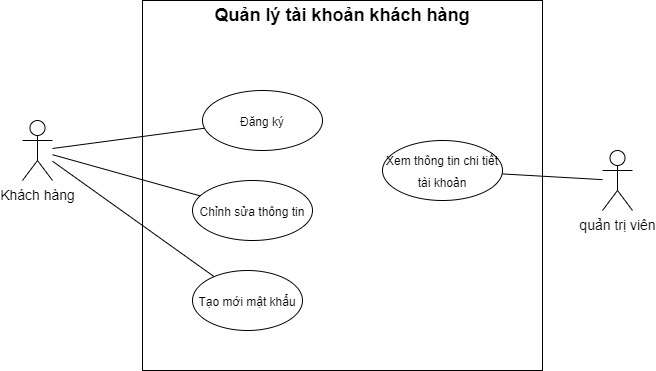
\includegraphics[width=9cm]{img/UseCase/UseCase-Quản lý tài khoản.drawio.png}
    \newline
    \caption{Use case quản lý tài khoản}
\end{figure}

\subsubsection{Đăng ký}
{
    \setlength\extrarowheight{6pt}
    \begin{longtable}{| p{.20\textwidth} | p{.80\textwidth} |}
        \hline
        \textbf{Use-case name}
         &
        Đăng ký
        \\
        %%%%%%%%%%%%%%%%%%
        \hline
        \textbf{Actor}
         &
        Khách hàng
        \\
        %%%%%%%%%%%%%%%%%%
        \hline
        \textbf{Description}
         &
        Khách hàng có thể đăng ký tài khoản
        \\
        %%%%%%%%%%%%%%%%%%
        \hline
        \textbf{Preconditions}
         &
        Khách hàng truy cập hệ thống
        \\
        %%%%%%%%%%%%%%%%%%
        \hline
        \textbf{Postconditions}
         &
        Tài khoản được đăng ký
        \\
        %%%%%%%%%%%%%%%%%%
        \hline
        \textbf{Trigger}
         &
        Khách hàng chọn đăng ký
        \\
        %%%%%%%%%%%%%%%%%%
        \hline
        \begin{flushleft}
            \textbf{Normal flow}
        \end{flushleft}
         &
        1. Hệ thống hiển thị biểu mẫu thông tin khách hàng

        2. Khách hàng nhập thông tin của mình

        3. Khách hạng chọn đăng ký

        4. Hệ thống hiện yêu cầu nhập mã xác nhận

        5. Khách hàng nhập mã và chọn gửi

        6. Hệ thống cập nhật thông tin
        \\
        %%%%%%%%%%%%%%%%%%
        \hline
        \begin{flushleft}
            \textbf{Alternative flow}
        \end{flushleft}
         &
        3.1. Khách hàng chọn hủy
        \begin{quote}
            3.1.1 Kết thúc
        \end{quote}
        \\
        %%%%%%%%%%%%%%%%%%
        \hline
        \begin{flushleft}
            \textbf{Exceptions}
        \end{flushleft}
         &
        4.1. Số điện thoại đã được sử dụng
        \begin{quote}
            4.1.1 Quay lại bước 1
        \end{quote}
        6.1. Khách hàng nhập sai OTP
        \begin{quote}
            6.1.1 Quay lại bước 5
        \end{quote}
        \\
        %%%%%%%%%%%%%%%%%%
        \hline
        \caption{Đặc tả use-case \textbf{Đăng ký}}
    \end{longtable}
}

\subsubsection{Chỉnh sửa thông tin}
{
    \setlength\extrarowheight{6pt}
    \begin{longtable}{| p{.20\textwidth} | p{.80\textwidth} |}
        \hline
        \textbf{Use-case name}
         &
        Chỉnh sửa thông tin
        \\
        %%%%%%%%%%%%%%%%%%
        \hline
        \textbf{Actor}
         &
        Khách hàng
        \\
        %%%%%%%%%%%%%%%%%%
        \hline
        \textbf{Description}
         &
        Khách hàng có thể chỉnh sửa thông tin cá nhân
        \\
        %%%%%%%%%%%%%%%%%%
        \hline
        \textbf{Preconditions}
         &
        Khách hàng đã đăng nhập
        \\
        %%%%%%%%%%%%%%%%%%
        \hline
        \textbf{Postconditions}
         &
        Thông tin được cập nhật
        \\
        %%%%%%%%%%%%%%%%%%
        \hline
        \textbf{Trigger}
         &
        Khách hàng chọn vào tài khoản
        \\
        %%%%%%%%%%%%%%%%%%
        \hline
        \begin{flushleft}
            \textbf{Normal flow}
        \end{flushleft}
         &
        1. Hệ thống hiển thị biểu mẫu thông tin tài khoản

        2. Khách hàng chỉnh sửa thông tin tài khoản

        3. Khách hàng chọn lưu

        4. Hệ thống cập nhật thông tin
        \\
        %%%%%%%%%%%%%%%%%%
        \hline
        \begin{flushleft}
            \textbf{Alternative flow}
        \end{flushleft}
         &
        3.1.Khách hàng chọn hủy
        \begin{quote}
            3.1.1 Kết thúc
        \end{quote}
        \\
        %%%%%%%%%%%%%%%%%%
        \hline
        \textbf{Exceptions}
         &
        Không
        \\
        %%%%%%%%%%%%%%%%%%
        \hline
        \caption{Đặc tả use-case \textbf{Chỉnh sửa thông tin}}
    \end{longtable}
}

\subsubsection{Tạo mới mật khẩu}
{
    \setlength\extrarowheight{6pt}
    \begin{longtable}{| p{.20\textwidth} | p{.80\textwidth} |}
        \hline
        \textbf{Use-case name}
         &
        Tạo mới mật khẩu
        \\
        %%%%%%%%%%%%%%%%%%
        \hline
        \textbf{Actor}
         &
        Khách hàng
        \\
        %%%%%%%%%%%%%%%%%%
        \hline
        \textbf{Description}
         &
        Khách hàng có thể cập nhật mật khẩu mới khi quên mật khẩu
        \\
        %%%%%%%%%%%%%%%%%%
        \hline
        \textbf{Preconditions}
         &
        Khách hàng đã truy cập hệ thống
        \\
        %%%%%%%%%%%%%%%%%%
        \hline
        \textbf{Postconditions}
         &
        Thông tin được cập nhật
        \\
        %%%%%%%%%%%%%%%%%%
        \hline
        \textbf{Trigger}
         &
        Khách hàng chọn vào quên mật khẩu
        \\
        %%%%%%%%%%%%%%%%%%
        \hline
        \begin{flushleft}
            \textbf{Normal flow}
        \end{flushleft}
         &
        1. Hệ thống yêu cầu thông tin liên hệ

        2. Khách hàng nhập thông tin và gửi

        3. Hệ thống yêu cầu nhập mã xác nhận

        4. Khách hàng nhập mã và chọn gửi

        5. Hệ thống yêu cầu nhập mật khẩu mới

        6. Khách hàng nhập mật khẩu mới và chọn xác nhận

        7. Hệ thống cập nhật thông tin và hiển thị màn hình đăng nhập
        \\
        %%%%%%%%%%%%%%%%%%
        \hline
        \textbf{Alternative flow}
         &
        Không
        \\
        %%%%%%%%%%%%%%%%%%
        \hline
        \textbf{Exceptions}
         &
        6.1.  Khách hàng nhập sai OTP
        \begin{quote}
            6.1.1.Thông báo sai
            6.1.2 Quay lại bước 3
        \end{quote}
        \\
        %%%%%%%%%%%%%%%%%%
        \hline
        \caption{Đặc tả use-case \textbf{Tạo mới mật khẩu}}
    \end{longtable}
}

\subsubsection{Đổi mật khẩu}
{
    \setlength\extrarowheight{6pt}
    \begin{longtable}{| p{.20\textwidth} | p{.80\textwidth} |}
        \hline
        \textbf{Use-case name}
         &
        Đổi mật khẩu
        \\
        %%%%%%%%%%%%%%%%%%
        \hline
        \textbf{Actor}
         &
        Khách hàng, nhân viên
        \\
        %%%%%%%%%%%%%%%%%%
        \hline
        \textbf{Description}
         &
        Người dùng có thể đổi mật khẩu mới cho tài khoản
        \\
        %%%%%%%%%%%%%%%%%%
        \hline
        \textbf{Preconditions}
         &
        Người dùng đã đăng nhập hệ thống
        \\
        %%%%%%%%%%%%%%%%%%
        \hline
        \textbf{Postconditions}
         &
        Thông tin được cập nhật
        \\
        %%%%%%%%%%%%%%%%%%
        \hline
        \textbf{Trigger}
         &
        Khách hàng chọn vào đổi mật khẩu
        \\
        %%%%%%%%%%%%%%%%%%
        \hline
        \begin{flushleft}
            \textbf{Normal flow}
        \end{flushleft}
         &
        1. Hệ thống hiển thị form đổi mật khẩu

        2. Người dùng nhập thông tin và gửi

        3. Hệ thống kiểm tra thông tin, cập nhật và thông báo
        \\
        %%%%%%%%%%%%%%%%%%
        \hline
        \textbf{Alternative flow}
         &
        Không
        \\
        %%%%%%%%%%%%%%%%%%
        \hline
        \textbf{Exceptions}
         &
        Không
        \\
        %%%%%%%%%%%%%%%%%%
        \hline
        \caption{Đặc tả use-case \textbf{Đổi mật khẩu}}
    \end{longtable}
}



\subsection{Quản lý kho}
\begin{figure}[!htp]
    \centering
    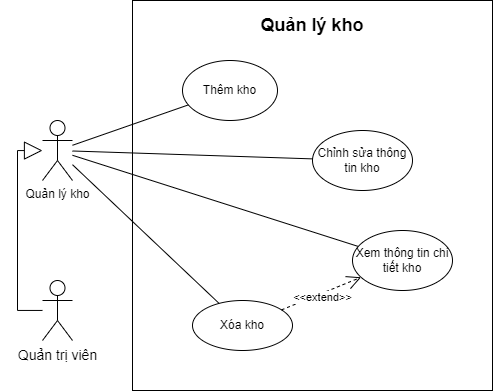
\includegraphics[width=9cm]{img/UseCase/UseCase-Quản lý kho.drawio.png}
    \newline
    \caption{Use case quản lý kho}
\end{figure}


\subsubsection{Thêm kho}
{
    \setlength\extrarowheight{6pt}
    \begin{longtable}{| p{.20\textwidth} | p{.80\textwidth} |}
        \hline
        \textbf{Use-case name}
         &
        Thêm kho.
        \\
        \hline
        \textbf{Actor}
         &
        Quản lý kho.
        \\
        \hline
        \textbf{Description}
         &
        Quản lý thêm kho mới vào trong hệ thống lưu trữ.
        \\
        \hline
        \textbf{Preconditions}
         &
        Quản lý kho đã đăng nhập vào hệ thống.
        \\
        \hline
        \textbf{Postconditions}
         &
        Quản lý thêm được kho mà quản lý kho muốn.
        \\
        \hline
        \textbf{Trigger}
         &
        Quản lý kho chọn nút "Quản lý kho".
        \\
        \hline
        \begin{flushleft}
            \textbf{Normal flow}
        \end{flushleft}
         &
        1. Hệ thống hiển thị danh sách tất cả kho.
        2. Quản lý kho chọn nút "Thêm kho".

        3. Hệ thống hiển thị thông tin kho cần điền thông tin để thêm.

        4. Người dùng nhập thông tin của kho và nhấn "Tạo".

        5. Hệ thống tiến hành kiểm tra định dạng các thông tin mà người dùng chọn và thông báo kết quả tạo kho thành công.

        6. Người dùng xem kết quả tạo kho.
        \\
        \hline
        \textbf{Alternative flow}
         &
        Không.
        %%%%%%%%%%%%%%%%
        \\
        \hline
        \textbf{Exceptions}
         &
        5.1. Người dùng nhập thông tin không đúng định dạng.
        \begin{quote}
            5.1.1. Hệ thống thông báo thông tin kho nhập vào sai định dạng, yêu cầu người dùng nhập lại.

            5.1.2. Người dùng chỉnh sửa lại các thông tin theo định dạng và chọn "Tạo".

            5.1.3.Quay lại bước 5.
        \end{quote}
        5.2. Tạo kho thất bại.
        \begin{quote}
            5.2.1. Hệ thống thông báo kết quả tạo kho thất bại.
            5.2.2. Quay lại bước 2.
        \end{quote}
        %%%%%%%%%%%%%%%%%%%%
        \\
        \hline
        \caption{Đặc tả use-case \textbf{thêm kho}}
    \end{longtable}
}

\subsubsection{Chỉnh sửa thông tin kho}
{
    \setlength\extrarowheight{6pt}
    \begin{longtable}{| p{.20\textwidth} | p{.80\textwidth} |}
        \hline
        \textbf{Use-case name}
         &
        Chỉnh sửa thông tin kho.
        \\
        \hline
        \textbf{Actor}
         &
        Quản lý kho.
        \\
        \hline
        \textbf{Description}
         &
        Quản lý chỉnh sửa thông tin kho.
        \\
        \hline
        \textbf{Preconditions}
         &
        Quản lý kho đã đăng nhập vào hệ thống.
        \\
        \hline
        \textbf{Postconditions}
         &
        Quản lý chỉnh sửa được thông tin của kho mà quản lý kho muốn.
        \\
        \hline
        \textbf{Trigger}
         &
        Quản lý chọn nút "Quản lý kho".
        \\
        \hline
        \begin{flushleft}
            \textbf{Normal flow}
        \end{flushleft}
         &
        1. Hệ thống hiển thị danh sách tất cả kho.

        2. Quản lý kho chọn kho muốn chỉnh sửa thông tin và nhấn nút "Chỉnh sửa".

        3. Hệ thống hiển thị thông tin kho có sẵn.

        4. Người dùng chỉnh sửa thông tin của kho và nhấn "Lưu".

        5. Hệ thống tiến hành kiểm tra định dạng các thông tin mà người dùng chọn và thông báo kết quả chỉnh sửa kho thành công.

        6. Người dùng xem kết quả chỉnh sửa kho.
        \\
        \hline
        \begin{flushleft}
            \textbf{Alternative flow}
        \end{flushleft}
         &
        1.1. Quản lý kho muốn chỉnh sửa sau khi xem thông tin chi tiết của kho.
        \begin{quote}
            1.1.1. Quản lý kho chọn nút "Chỉnh sửa" trong trang xem thông tin chi tiết kho.
            1.1.2. Đến bước 3.
        \end{quote}
        %%%%%%%%%%%%%%%%
        \\
        \hline
        \begin{flushleft}
            \textbf{Exceptions}
        \end{flushleft}
         &
        5.1. Người dùng nhập thông tin không đúng định dạng.
        \begin{quote}
            5.1.1. Hệ thống thông báo thông tin kho nhập vào sai định dạng, yêu cầu người dùng nhập lại.
            5.1.2. Người dùng chỉnh sửa lại các thông tin theo định dạng và chọn "Lưu".
            5.1.3. Quay lại bước 5.
        \end{quote}
        5.2. Hệ thống chỉnh sửa kho thất bại.
        \begin{quote}
            5.2.1. Hệ thống thông báo kết quả chỉnh sửa kho thất bại.
            5.2.2. Quay lại bước 2.
        \end{quote}
        %%%%%%%%%%%%%%%%%%%%
        \\
        \hline
        \caption{Đặc tả use-case \textbf{chỉnh sửa thông tin kho}}
    \end{longtable}
}


\subsection{Quản lý hàng hóa}
\begin{figure}[!htp]
    \centering
    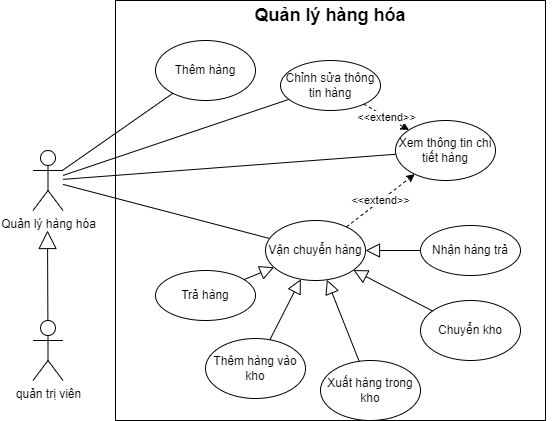
\includegraphics[width=10cm]{img/UseCase/UseCase-Quản lý hàng.drawio.png}
    \newline
    \caption{Use case quản lý hàng hóa}
\end{figure}


\subsubsection{Thêm hàng}
{
    \setlength\extrarowheight{6pt}
    \begin{longtable}{| p{.20\textwidth} | p{.80\textwidth} |}
        \hline
        \textbf{Use-case name}
         &
        Thêm hàng
        \\
        %%%%%%%%%%%%%%%%%%
        \hline
        \textbf{Actor}
         &
        Quản lý hàng hóa
        \\
        %%%%%%%%%%%%%%%%%%
        \hline
        \textbf{Description}
         &
        Quản lý hàng hóa có thể thêm vào hệ thống
        \\
        %%%%%%%%%%%%%%%%%%
        \hline
        \textbf{Preconditions}
         &
        Quản lý hàng hóa đã đăng nhập
        \\
        %%%%%%%%%%%%%%%%%%
        \hline
        \textbf{Postconditions}
         &
        Hàng được thêm vào hệ thống
        \\
        %%%%%%%%%%%%%%%%%%
        \hline
        \textbf{Trigger}
         &
        Quản lý hàng hóa chọn "Quản lý hàng hóa"
        \\
        %%%%%%%%%%%%%%%%%%
        \hline
        \begin{flushleft}
            \textbf{Normal flow}
        \end{flushleft}
         &
        1. Hệ thống hiển thị danh sách hàng hóa

        2. Quản lý chọn thêm mới

        3. Hệ thống hiển thị trang thêm mới hàng

        4. Quản lý hàng hóa nhập thông tin hàng

        5. Quản lý hàng hóa chọn "Lưu"

        6. Hệ thống cập nhật thông tin
        \\
        %%%%%%%%%%%%%%%%%%
        \hline
        \begin{flushleft}
            \textbf{Alternative flow}
        \end{flushleft}
         &
        5.1. Quản lý hàng hóa chọn "Hủy"
        \begin{quote}

            5.1.1 Quay lại bước 1
        \end{quote}
        \\
        %%%%%%%%%%%%%%%%%%
        \hline
        \textbf{Exceptions}
         &
        Không
        \\
        %%%%%%%%%%%%%%%%%%
        \hline
        \caption{Đặc tả use-case \textbf{Thêm hàng}}
    \end{longtable}
}

\subsubsection{Chỉnh sửa thông tin hàng}
{
    \setlength\extrarowheight{6pt}
    \begin{longtable}{| p{.20\textwidth} | p{.80\textwidth} |}
        \hline
        \textbf{Use-case name}
         &
        Chỉnh sửa thông tin hàng
        \\
        %%%%%%%%%%%%%%%%%%
        \hline
        \textbf{Actor}
         &
        Quản lý hàng hóa
        \\
        %%%%%%%%%%%%%%%%%%
        \hline
        \textbf{Description}
         &
        Quản lý hàng hóa có thể thông tin đầy đủ của hàng
        \\
        %%%%%%%%%%%%%%%%%%
        \hline
        \textbf{Preconditions}
         &
        Quản lý hàng hóa đã đăng nhập
        \\
        %%%%%%%%%%%%%%%%%%
        \hline
        \textbf{Postconditions}
         &
        Thông tin hàng được cập nhật
        \\
        %%%%%%%%%%%%%%%%%%
        \hline
        \textbf{Trigger}
         &
        Quản lý hàng hóa chọn "Quản lý hàng hóa"
        \\
        %%%%%%%%%%%%%%%%%%
        \hline
        \begin{flushleft}
            \textbf{Normal flow}
        \end{flushleft}
         &
        1. Hệ thống hiển thị danh sách hàng hóa

        2. Quản lý hàng hóa tìm kiếm và chọn hàng muốn chỉnh sửa

        3. Thông tin chi tiết hàng được hiển thị

        4. Quản lý hàng hóa chọn "Chỉnh sửa"

        5. Hệ thống hiển thị biểu mẫu thông tin hàng

        6. Quản lý hàng hóa nhập thông tin

        7. Quản lý hàng hóa chọn "Lưu"

        8. Hệ thống cập nhật thông tin
        \\
        %%%%%%%%%%%%%%%%%%
        \hline
        \begin{flushleft}
            \textbf{Alternative flow}
        \end{flushleft}
         &
        7.1 Quản lý hàng hóa chọn "Hủy"
        \begin{quote}
            7.1.1 Quay lại bước 3
        \end{quote}
        \\
        %%%%%%%%%%%%%%%%%%
        \hline
        \textbf{Exceptions}
         &
        Không
        \\
        %%%%%%%%%%%%%%%%%%
        \hline
        \caption{Đặc tả use-case \textbf{Chỉnh sửa thông tin chi tiết hàng}}
    \end{longtable}
}

\subsubsection{Thêm hàng vào kho}
{
    \setlength\extrarowheight{6pt}
    \begin{longtable}{| p{.20\textwidth} | p{.80\textwidth} |}
        \hline
        \textbf{Use-case name}
         &
        Thêm hàng vào kho
        \\
        %%%%%%%%%%%%%%%%%%
        \hline
        \textbf{Actor}
         &
        Quản lý hàng hóa
        \\
        %%%%%%%%%%%%%%%%%%
        \hline
        \textbf{Description}
         &
        Quản lý hàng hóa có thể thêm hàng vào kho
        \\
        %%%%%%%%%%%%%%%%%%
        \hline
        \textbf{Preconditions}
         &
        Quản lý hàng hóa đã đăng nhập
        \\
        %%%%%%%%%%%%%%%%%%
        \hline
        \textbf{Postconditions}
         &
        Hàng được thêm
        \\
        %%%%%%%%%%%%%%%%%%
        \hline
        \textbf{Trigger}
         &
        Quản lý hàng hóa chọn "Quản lý hàng hóa"
        \\
        %%%%%%%%%%%%%%%%%%
        \hline
        \begin{flushleft}
            \textbf{Normal flow}
        \end{flushleft}
         &
        1. Hệ thống hiển thị danh sách hàng hóa

        2. Quản lý hàng hóa tìm kiếm và chọn hàng muốn xuất

        3. Thông tin chi tiết hàng được hiển thị

        4. Quản lý hàng hóa chọn vào "Nhập kho"

        5. Quản lý hàng hóa nhập thông tin

        6. Quản lý hàng hóa chọn "Thực hiện"

        7. Hệ thống cập nhật thông tin
        \\
        %%%%%%%%%%%%%%%%%%
        \hline
        \begin{flushleft}
            \textbf{Alternative flow}
        \end{flushleft}
         &
        5.1. Quản lý hàng hóa chọn hủy
        \begin{quote}
            5.1.1 Quay lại bước 3
        \end{quote}
        \\
        %%%%%%%%%%%%%%%%%%
        \hline
        \textbf{Exceptions}
         &
        Không
        \\
        %%%%%%%%%%%%%%%%%%
        \hline
        \caption{Đặc tả use-case \textbf{Thêm hàng vào kho}}
    \end{longtable}
}


\subsubsection{Xuất hàng trong kho}
{
    \setlength\extrarowheight{6pt}
    \begin{longtable}{| p{.20\textwidth} | p{.80\textwidth} |}
        \hline
        \textbf{Use-case name}
         &
        Xuất hàng trong kho
        \\
        %%%%%%%%%%%%%%%%%%
        \hline
        \textbf{Actor}
         &
        Quản lý hàng hóa
        \\
        %%%%%%%%%%%%%%%%%%
        \hline
        \textbf{Description}
         &
        Quản lý hàng hóa có thể xuất hảng khỏi kho
        \\
        %%%%%%%%%%%%%%%%%%
        \hline
        \textbf{Preconditions}
         &
        Quản lý hàng hóa đã đăng nhập
        \\
        %%%%%%%%%%%%%%%%%%
        \hline
        \textbf{Postconditions}
         &
        Hàng được xuất khỏi kho
        \\
        %%%%%%%%%%%%%%%%%%
        \hline
        \textbf{Trigger}
         &
        Quản lý hàng hóa chọn "Quản lý hàng hóa"
        \\
        %%%%%%%%%%%%%%%%%%
        \hline
        \begin{flushleft}
            \textbf{Normal flow}
        \end{flushleft}
         &
        1. Hệ thống hiển thị danh sách hàng hóa

        2. Quản lý hàng hóa tìm kiếm và chọn hàng muốn xuất

        3.Thông tin chi tiết hàng được hiển thị

        4. Quản lý hàng hóa tìm kiếm và chọn kho muốn xuất

        5. Hệ thống hiển thị biểu mẫu thông tin quy trình

        6. Quản lý hàng hóa nhập thông tin

        7. Quản lý hàng hóa chọn "Thực hiện"

        8. Hệ thống cập nhật thông tin
        \\
        %%%%%%%%%%%%%%%%%%
        \hline
        \textbf{Alternative flow}
         &
        Không
        \\
        %%%%%%%%%%%%%%%%%%
        \hline
        \textbf{Exceptions}
         &
        Không
        \\
        %%%%%%%%%%%%%%%%%%
        \hline
        \caption{Đặc tả use-case \textbf{Xuất hàng trong kho}}
    \end{longtable}
}


\subsubsection{Chuyển kho}
{
    \setlength\extrarowheight{6pt}
    \begin{longtable}{| p{.20\textwidth} | p{.80\textwidth} |}
        \hline
        \textbf{Use-case name}
         &
        Chuyển kho
        \\
        %%%%%%%%%%%%%%%%%%
        \hline
        \textbf{Actor}
         &
        Quản lý hàng hóa
        \\
        %%%%%%%%%%%%%%%%%%
        \hline
        \textbf{Description}
         &
        Quản lý hàng hóa có thể chuyển hàng từ kho này đến kho khác
        \\
        %%%%%%%%%%%%%%%%%%
        \hline
        \textbf{Preconditions}
         &
        Quản lý hàng hóa đã đăng nhập
        \\
        %%%%%%%%%%%%%%%%%%
        \hline
        \textbf{Postconditions}
         &
        Hàng chuyển đi
        \\
        %%%%%%%%%%%%%%%%%%
        \hline
        \textbf{Trigger}
         &
        Quản lý hàng hóa chọn "Quản lý hàng hóa"
        \\
        %%%%%%%%%%%%%%%%%%
        \hline
        \begin{flushleft}
            \textbf{Normal flow}
        \end{flushleft}
         &
        1. Hệ thống hiển thị danh sách hàng hóa

        2. Quản lý hàng hóa tìm kiếm và chọn hàng muốn xuất

        3. Thông tin chi tiết hàng được hiển thị

        4. Quản lý hàng hóa tìm kiếm và chọn kho muốn xuất

        5. Hệ thống hiển thị biểu mẫu thông tin quy trình

        6. Quản lý hàng hóa nhập thông tin

        7. Quản lý hàng hóa chọn "Thực hiện"

        8. Hệ thống cập nhật thông tin
        \\
        %%%%%%%%%%%%%%%%%%
        \hline
        \textbf{Alternative flow}
         &
        Không
        \\
        %%%%%%%%%%%%%%%%%%
        \hline
        \textbf{Exceptions}
         &
        Không
        \\
        %%%%%%%%%%%%%%%%%%
        \hline
        \caption{Đặc tả use-case \textbf{Chuyển kho}}
    \end{longtable}
}

\subsubsection{Nhận trả hàng}
{
    \setlength\extrarowheight{6pt}
    \begin{longtable}{| p{.20\textwidth} | p{.80\textwidth} |}
        \hline
        \textbf{Use-case name}
         &
        Nhận trả hàng
        \\
        %%%%%%%%%%%%%%%%%%
        \hline
        \textbf{Actor}
         &
        Quản lý hàng hóa
        \\
        %%%%%%%%%%%%%%%%%%
        \hline
        \textbf{Description}
         &
        Quản lý hàng hóa có thể chuyển hàng từ kho này đến kho khác
        \\
        %%%%%%%%%%%%%%%%%%
        \hline
        \textbf{Preconditions}
         &
        Quản lý hàng hóa đã đăng nhập
        \\
        %%%%%%%%%%%%%%%%%%
        \hline
        \textbf{Postconditions}
         &
        Hàng chuyển đi
        \\
        %%%%%%%%%%%%%%%%%%
        \hline
        \textbf{Trigger}
         &
        Quản lý hàng hóa chọn "Quản lý hàng hóa"
        \\
        %%%%%%%%%%%%%%%%%%
        \hline
        \begin{flushleft}
            \textbf{Normal flow}
        \end{flushleft}
         &
        1. Hệ thống hiển thị danh sách hàng hóa

        2. Quản lý hàng hóa tìm kiếm và chọn hàng muốn xuất

        3. Thông tin chi tiết hàng được hiển thị

        4. Quản lý hàng hóa tìm kiếm và chọn kho muốn xuất

        5. Hệ thống hiển thị biểu mẫu thông tin quy trình

        6. Quản lý hàng hóa nhập thông tin

        7. Quản lý hàng hóa chọn "Thực hiện"

        8. Hệ thống cập nhật thông tin
        \\
        %%%%%%%%%%%%%%%%%%
        \hline
        \textbf{Alternative flow}
         &
        Không
        \\
        %%%%%%%%%%%%%%%%%%
        \hline
        \textbf{Exceptions}
         &
        Không
        \\
        %%%%%%%%%%%%%%%%%%
        \hline
        \caption{Đặc tả use-case \textbf{Nhận trả hàng}}
    \end{longtable}
}

\newpage

\subsection{Quản lý đơn hàng}
\begin{figure}[!htp]
    \centering
    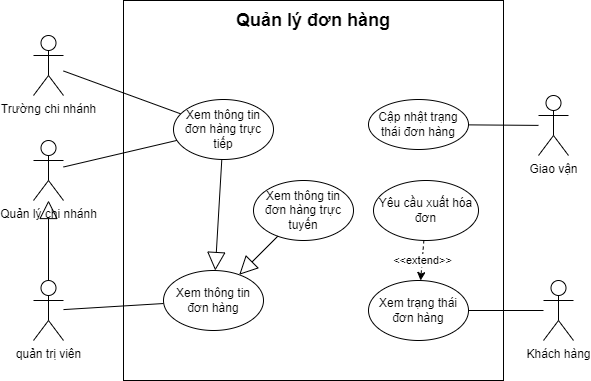
\includegraphics[width=5in]{img/UseCase/UseCase-Quản lý đơn hàng.drawio.png}
    \newline
    \caption{Use case quản lý đơn hàng}
\end{figure}

\subsubsection{Xem thông tin đơn hàng trực tiếp}
{
    \setlength\extrarowheight{6pt}
    \begin{longtable}{| p{.20\textwidth} | p{.80\textwidth} |}
        \hline
        \textbf{Use-case name}
         &
        Xem thông tin đơn hàng trực tiếp
        \\
        %%%%%%%%%%%%%%%%%%
        \hline
        \textbf{Actor}
         &
        Quản lý chi nhánh, trưởng chi nhánh
        \\
        %%%%%%%%%%%%%%%%%%
        \hline
        \textbf{Description}
         &
        Quản lý chi nhánh, trưởng chi nhánh có thể xem thông tin các đơn hàng
        \\
        %%%%%%%%%%%%%%%%%%
        \hline
        \textbf{Preconditions}
         &
        Quản lý chi nhánh, trưởng chi nhánh đã đăng nhập
        \\
        %%%%%%%%%%%%%%%%%%
        \hline
        \textbf{Postconditions}
         &
        Nhận được thông tin đơn hàng
        \\
        %%%%%%%%%%%%%%%%%%
        \hline
        \textbf{Trigger}
         &
        Quản lý chi nhánh, trưởng chi nhánh chọn "Quản lý đơn hàng"
        \\
        %%%%%%%%%%%%%%%%%%
        \hline
        \begin{flushleft}
            \textbf{Normal flow}
        \end{flushleft}
         &
        1. Quản lý chi nhánh, trưởng chi nhánh chọn khoảng thời gian muốn xem

        2. Hệ thống hiển thị danh sách các đơn hàng

        3. Quản lý chi nhánh, trưởng chi nhánh tìm và chọn đơn muốn xem

        4. Hệ thống hiển thị thông tin đơn hàng
        \\
        %%%%%%%%%%%%%%%%%%
        \hline
        \textbf{Alternative flow}
         &
        Không
        \\
        %%%%%%%%%%%%%%%%%%
        \hline
        \textbf{Exceptions}
         &
        Không
        \\
        %%%%%%%%%%%%%%%%%%
        \hline
        \caption{Đặc tả use-case \textbf{Xem thông tin đơn hàng trực tiếp}}
    \end{longtable}
}

\subsubsection{Xem thông tin đơn hàng trực tuyến}
{
    \setlength\extrarowheight{6pt}
    \begin{longtable}{| p{.20\textwidth} | p{.80\textwidth} |}
        \hline
        \textbf{Use-case name}
         &
        Xem thông tin đơn hàng trực tuyến
        \\
        %%%%%%%%%%%%%%%%%%
        \hline
        \textbf{Actor}
         &
        Quản trị viên
        \\
        %%%%%%%%%%%%%%%%%%
        \hline
        \textbf{Description}
         &
        Quản trị viên có thể xem thông tin các đơn hàng trực tuyến
        \\
        %%%%%%%%%%%%%%%%%%
        \hline
        \textbf{Preconditions}
         &
        Quản trị viên đã đăng nhập
        \\
        %%%%%%%%%%%%%%%%%%
        \hline
        \textbf{Postconditions}
         &
        Nhận được thông tin đơn hàng
        \\
        %%%%%%%%%%%%%%%%%%
        \hline
        \textbf{Trigger}
         &
        Quản trị viên chọn "Đơn hàng trực tuyến" trong "Quản lý đơn hàng
        \\
        %%%%%%%%%%%%%%%%%%
        \hline
        \begin{flushleft}
            \textbf{Normal flow}
        \end{flushleft}
         &
        1. Quản trị viên chọn khoảng thời gian muốn xem

        2. Hệ thống hiển thị danh sách các đơn hàng

        3. Quản trị viên tìm và chọn đơn muốn xem

        4. Hệ thống hiển thị thông tin đơn hàng
        \\
        %%%%%%%%%%%%%%%%%%
        \hline
        \textbf{Alternative flow}
         &
        Không
        \\
        %%%%%%%%%%%%%%%%%%
        \hline
        \textbf{Exceptions}
         &
        Không
        \\
        %%%%%%%%%%%%%%%%%%
        \hline
        \caption{Đặc tả use-case \textbf{Xem thông tin đơn hàng trực tuyến}}
    \end{longtable}
}

\subsubsection{Cập nhật trạng thái đơn hàng}
{
    \setlength\extrarowheight{6pt}
    \begin{longtable}{| p{.20\textwidth} | p{.80\textwidth} |}
        \hline
        \textbf{Use-case name}
         &
        Cập nhật trạng thái đơn hàng.
        \\
        \hline
        \textbf{Actor}
         &
        Giao vận.
        \\
        \hline
        \textbf{Description}
         &
        Bên giao vận gửi trạng thái cập nhật đơn hàng khi có sự thay đổi trạng thái ngoài thực tế.
        \\
        \hline
        \textbf{Preconditions}
         &
        Bên giao vận gửi trạng thái cập nhật của đơn hàng.
        \\
        \hline
        \textbf{Postconditions}
         &
        Hệ thống ghi nhận trạng thái mới của đơn hàng.
        \\
        \hline
        \textbf{Trigger}
         &
        Không.
        \\
        \hline
        \textbf{Normal flow}
         &
        1. Bên giao vận gửi trạng thái cập nhật của đơn hàng

        2. Hệ thống ghi nhận cập nhật lại trạng thái mới cho đơn hàng.
        \\
        \hline
        \textbf{Alternative flow}
         &
        Không
        %%%%%%%%%%%%%%%%
        \\
        \hline
        \textbf{Exceptions}
         &
        Không
        %%%%%%%%%%%%%%%%%%%%
        \\
        \hline
        \caption{Đặc tả use-case \textbf{cập nhật trạng thái đơn hàng}}
    \end{longtable}
}

\subsubsection{Xem trạng thái đơn hàng}
{
    \setlength\extrarowheight{6pt}
    \begin{longtable}{| p{.20\textwidth} | p{.80\textwidth} |}
        \hline
        \textbf{Use-case name}
         &
        Xem trạng thái đơn hàng.
        \\
        \hline
        \textbf{Actor}
         &
        Khách hàng.
        \\
        \hline
        \textbf{Description}
         &
        Khách hàng xem trạng thái hiện tại của đơn hàng.
        \\
        \hline
        \textbf{Preconditions}
         &
        Khách hàng đã đăng nhập.
        \\
        \hline
        \textbf{Postconditions}
         &
        Khách hàng xem được trạng thái hiện tại của đơn hàng mà khách hàng muốn xem.
        \\
        \hline
        \textbf{Trigger}
         &
        Không.
        \\
        \hline
        \begin{flushleft}
            \textbf{Normal flow}

        \end{flushleft}
         &
        1. Khách hàng chọn vào mục "Quản lý đơn hàng".

        2. Hệ thống hiển thị danh sách các đơn hàng ở tab mặc định chưa giao hàng.

        3. Khách hàng lựa chọn đơn hàng mà mình muốn xem thông tin và nhấn vào đơn hàng đó.

        4. Hệ thống hiển thị thông tin chi tiết về trạng thái đơn hàng.

        5. Người dùng xem kết quả trạng thái đơn hàng mà mình muốn.
        \\
        \hline
        \begin{flushleft}
            \textbf{Alternative flow}
        \end{flushleft}
         &
        3.1. Khách hàng muốn xem các đơn hàng đã giao.
        \begin{quote}
            3.1.1. Khách hàng chọn mục "Đơn đã giao".

            3.1.2. Hệ thống hiển thị danh sách các đơn hàng đã giao của khách hàng.

            3.1.3. Quay lại bước 3.
        \end{quote}
        %%%%%%%%%%%%%%%%
        \\
        \hline
        \textbf{Exceptions}
         &
        Không
        %%%%%%%%%%%%%%%%%%%%
        \\
        \hline
        \caption{Đặc tả use-case \textbf{xem trạng thái đơn hàng}}
    \end{longtable}
}


\subsubsection{Yêu cầu xuất hóa đơn}
{
    \setlength\extrarowheight{6pt}
    \begin{longtable}{| p{.20\textwidth} | p{.80\textwidth} |}
        \hline
        \textbf{Use-case name}
         &
        Yêu cầu xuất hóa đơn.
        \\
        \hline
        \textbf{Actor}
         &
        Khách hàng.
        \\
        \hline
        \textbf{Description}
         &
        Khách hàng yêu cầu hệ thống xuất hóa đơn cho đơn hàng online.
        \\
        \hline
        \textbf{Preconditions}
         &
        Khách hàng đã từng mua hàng thành công trên trang bán hàng online.
        \\
        \hline
        \textbf{Postconditions}
         &
        Hệ thống gửi khách hàng hóa đơn của đơn hàng tương ứng.
        \\
        \hline
        \textbf{Trigger}
         &
        Không.
        \\
        \hline
        \begin{flushleft}
            \textbf{Normal flow}
        \end{flushleft}
         &
        1. Khách hàng chọn vào mục "Quản lý đơn hàng".

        2. Hệ thống hiển thị danh sách các đơn hàng ở tab mặc định chưa giao hàng.

        3. Khách hàng chọn mục "Đơn đã giao".

        4. Hệ thống hiển thị danh sách các đơn hàng đã giao của khách hàng.

        5. Khách hàng lựa chọn đơn hàng mà mình muốn xem thông tin và nhấn vào đơn hàng đó sau đó chọn "Yêu cầu xuất hóa đơn".

        6. Hệ thống thông báo kết quả và trả về tệp hóa đơn cho khách hàng.

        7. Người dùng xem kết quả trong tệp hóa đơn.
        \\
        \hline
        \textbf{Alternative flow}
         &
        Không
        %%%%%%%%%%%%%%%%
        \\
        \hline
        \begin{flushleft}
            \textbf{Exceptions}
        \end{flushleft}
         &
        3.1. Hệ thống tạo hóa đơn thất bại.
        \begin{quote}
            3.1.1. Quay lại bước 3.
        \end{quote}
        %%%%%%%%%%%%%%%%%%%%
        \\
        \hline
        \caption{Đặc tả use-case \textbf{yêu cầu xuất hóa đơn}}
    \end{longtable}
}




\newpage
% BPMN
% !TeX root = ..\main.tex
\section{Thiết kế lược đồ BPMN}

Các lược đồ BPMN được nhóm thiết kế trên app Bizagi.

\subsection{Quản lý kho}
\begin{figure}[!htp]
	\centering
	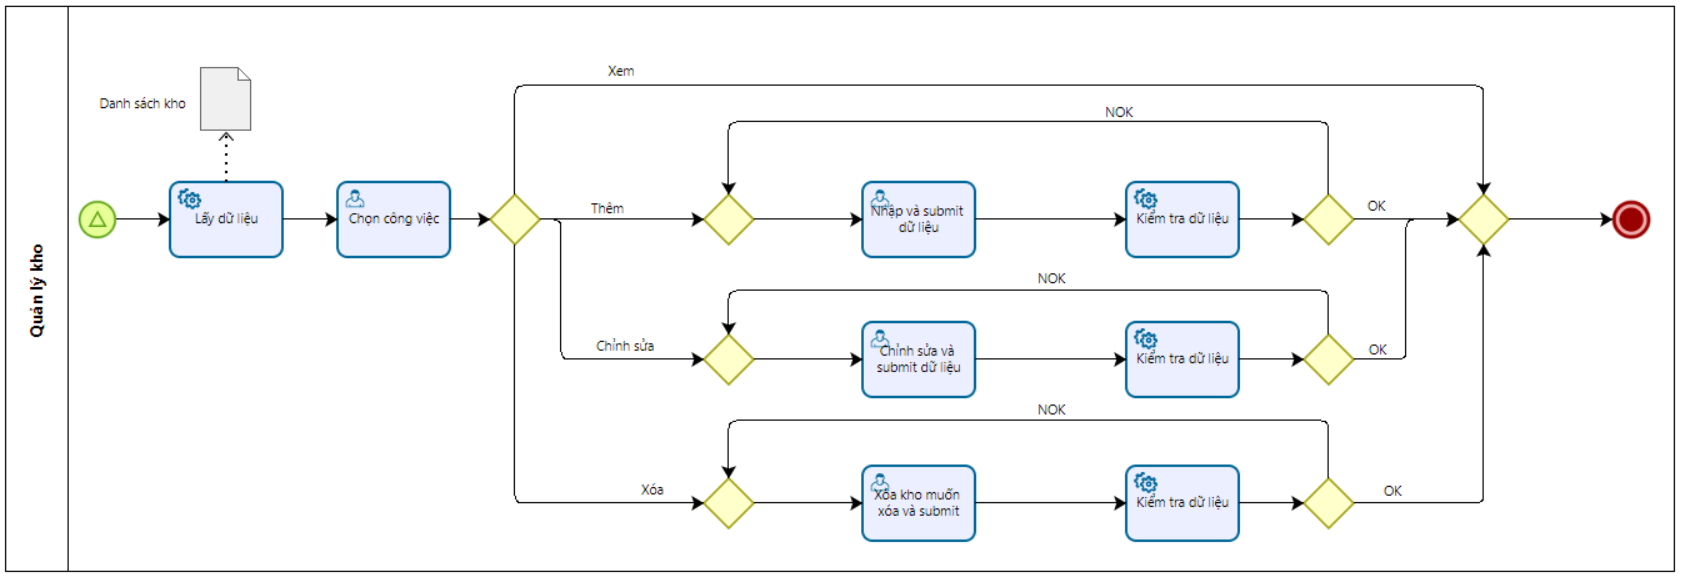
\includegraphics[width=17cm]{img/BPMN/Tho/warehouse.PNG}
	\newline
	\caption{Lược đồ BPMN cho quy trình quản lý kho}
\end{figure}

Quy trình bắt đầu khi người dùng truy cập vào giao diện quản lý kho. Hệ thống quản lý kho lấy ra dữ liệu kho cho người dùng thực hiện các tác vụ của mình. Nếu người dùng chỉ xem dữ liệu thì sẽ không có gì xảy ra thêm. Nếu người dùng thêm dữ liệu, người dùng sẽ nhập và submit dữ liệu mới, hệ thống kiểm tra và hoàn thành việc thêm nếu dữ liệu hợp lệ. Nếu người dùng chỉnh sửa dữ liệu, người dùng chỉnh sửa trên dữ liệu hiện tại của kho, hệ thống kiểm tra và hoàn thành việc cập nhật nếu dữ liệu hợp lệ. Nếu người dùng xóa dữ liệu, người dùng xóa kho và submit, hệ thống kiểm tra dữ liệu và hoàn thành việc xóa nếu dữ liệu hợp lệ.

\subsection{Lưu hóa đơn từ cửa hàng}
\begin{figure}[!htp]
	\centering
	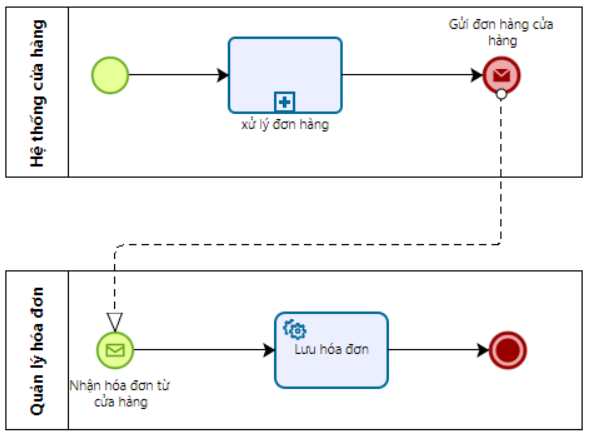
\includegraphics[width=8cm]{img/BPMN/Tho/save_invoice.PNG}
	\newline
	\caption{Lược đồ BPMN cho quy trình lưu hóa đơn từ cửa hàng}
\end{figure}

Quy trình bắt đầu sau khi cửa hàng xử lý xong đơn hàng và gửi thông tin đơn hàng cho hệ thống lưu lại. Hệ thống nhận dữ liệu và lưu lại đơn hàng vào hệ thống.

\newpage

\subsection{Khách hàng yêu cầu xuất hóa đơn}
\begin{figure}[!htp]
	\centering
	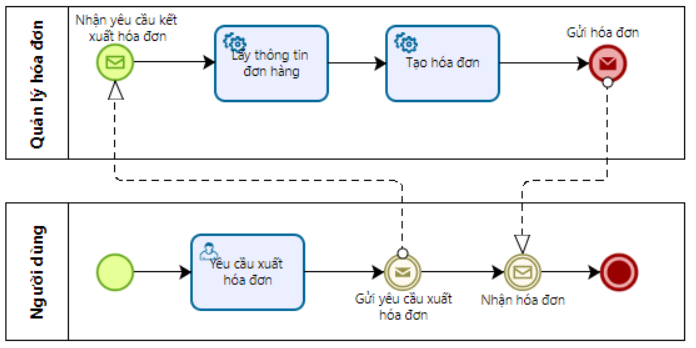
\includegraphics[width=10cm]{img/BPMN/Tho/invoice_log.PNG}
	\newline
	\caption{Lược đồ BPMN cho quy trình khách hàng yêu cầu xuất hóa đơn}
\end{figure}

Quy trình bắt đầu khi người dùng tạo yêu cầu xuất hóa đơn. Lúc đó bên quản lý đơn nhận được yêu cầu kết xuất hóa đơn, sau đó xử lý yêu cầu. Bên quản lý đơn lấy thông tin đơn hàng, sau đó tạo hóa đơn rồi gửi về lại cho khách hàng. Khách hàng nhận được hóa đơn như đã yêu cầu.

\subsection{Cập nhật trạng thái đơn hàng}
\begin{figure}[!htp]
	\centering
	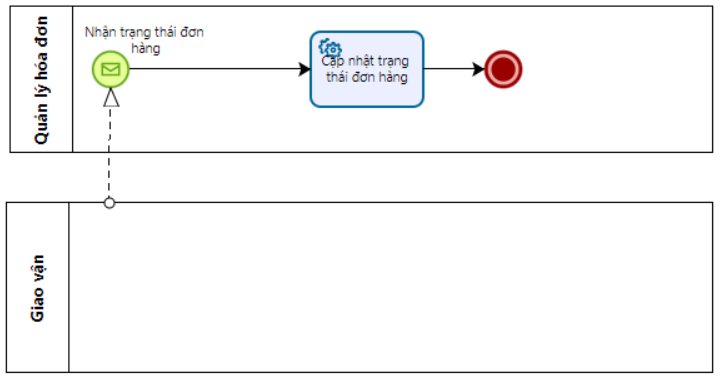
\includegraphics[width=9cm]{img/BPMN/Tho/update_status.PNG}
	\newline
	\caption{Lược đồ BPMN cho quy trình cập nhật trạng thái đơn hàng}
\end{figure}

Quy trình bắt đầu khi bên giao vận gửi dữ liệu cập nhật trạng thái mới của đơn hàng về cho hệ thống quản lý đơn. Bên quản lý đơn sau khi nhận được trạng thái đơn hàng đã cập nhật sẽ tiến hành cập nhật trạng thái đơn hàng trong hệ thống.

\subsection{Khách hàng mua hàng}
\begin{figure}[!htp]
    \centering
    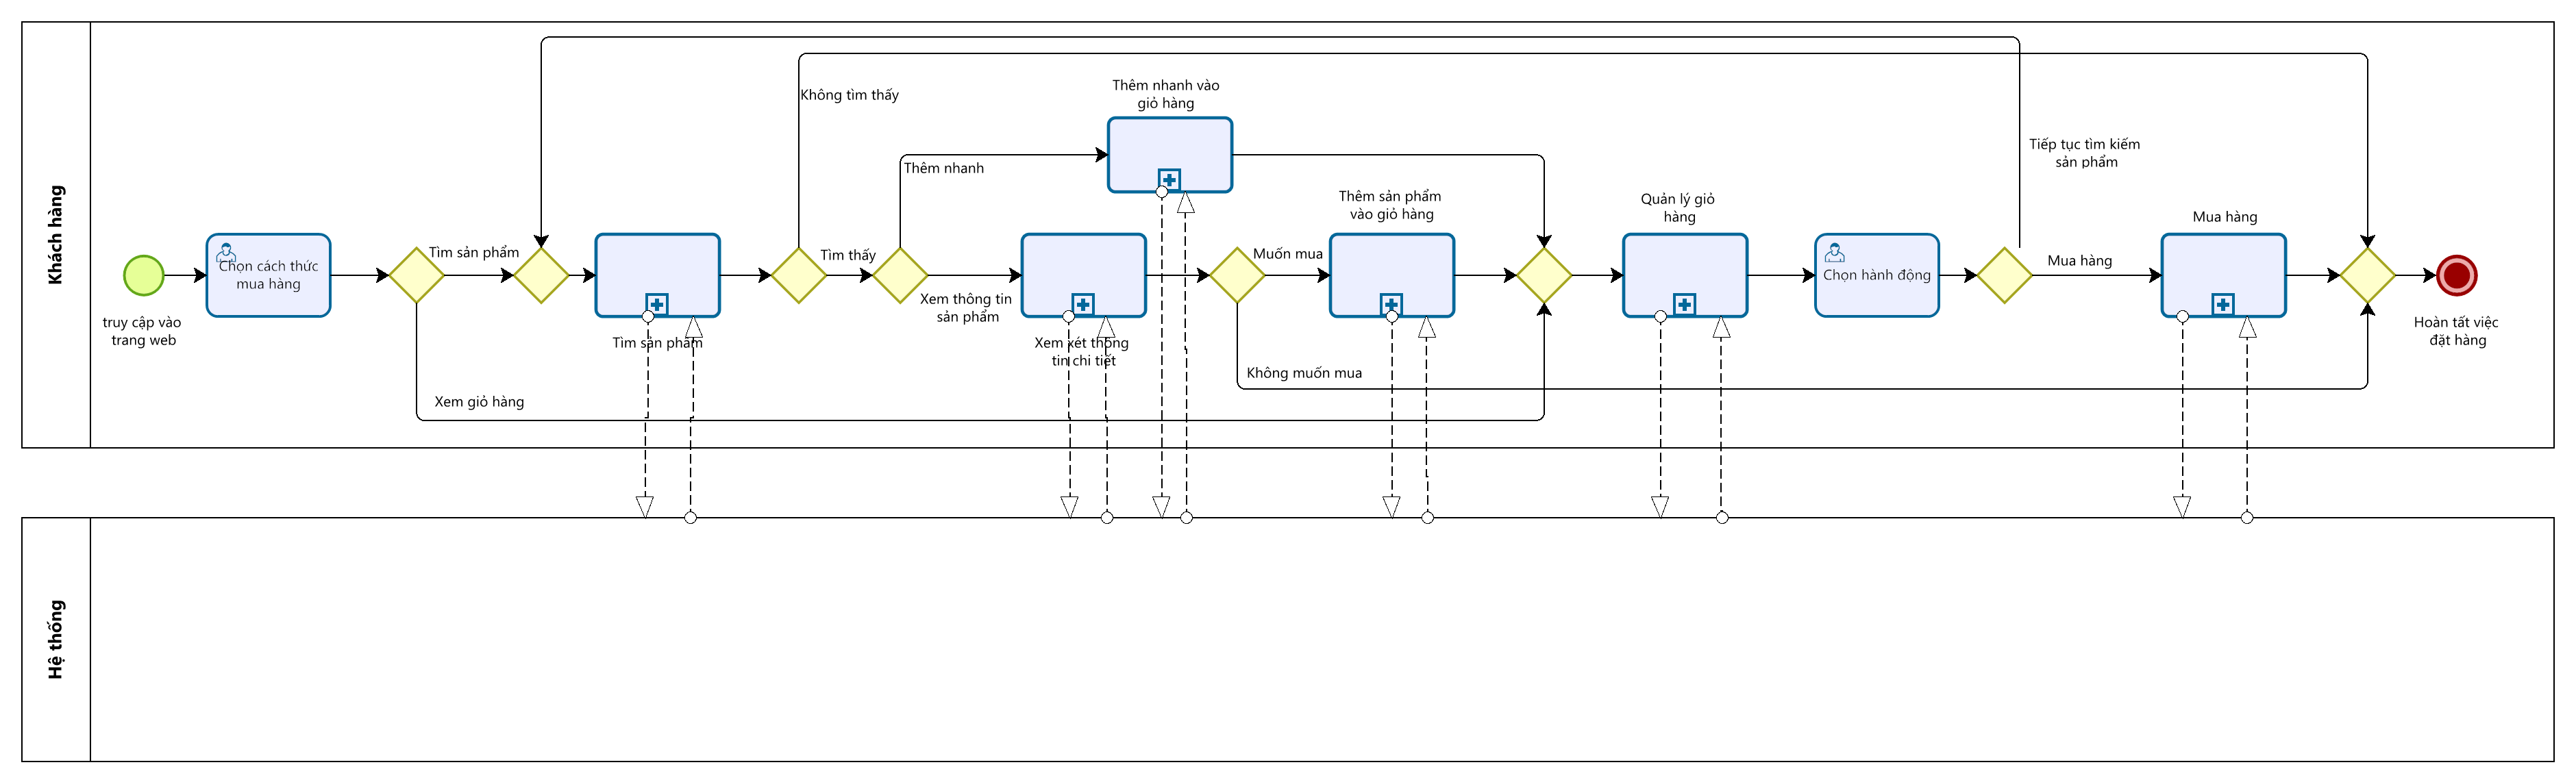
\includegraphics[width=17cm]{img/BPMN/customer_buy/customer_buy.png}
    \newline
    \caption{Lược đồ BPMN cho quy trình khách hàng mua hàng}
\end{figure}
 
Quy trình bắt đầu khi người dùng bắt đầu truy cập vào trang web, khách hàng chọn cách thức mua hàng là bắt đầu từ tìm sản phẩm hoặc là bắt đầu mua từ những sản phẩm đã có sẵn trong giỏ hàng. Khi người dùng chọn tìm sản phẩm thì người dùng sẽ thực hiện quy trình con (sub-process) "Tìm sản phẩm". Sau khi thực hiện xong tìm sản phẩm và tìm thấy thì người dùng thực hiện xem thông tin chi tiết để hiểu rõ hơn về sản phẩm và quyết định có muốn thêm sản phẩm vào giỏ hàng hay không; hoặc khi người dùng đã biết về sản phẩm thì có thể thêm chọn thêm nhanh sản phẩm vào giỏ hàng. Sau khi thêm sản phẩm vào giỏ hàng thì người dùng thực hiện quy trình con quản lý giỏ hàng để lựa chọn cũng như cập nhật các đặc điểm mà người dùng mong muốn ở sản phẩm. Sau khi quản lý xong giỏ hàng thì người dùng cần chọn hành động tiếp tục tìm kiếm thêm sản phẩm để mua hàng hoặc là trực tiếp đi đến quy trình con "Mua hàng" và sau đó là kết thúc quy trình.
 
 
\begin{figure}[!htp]
    \centering
    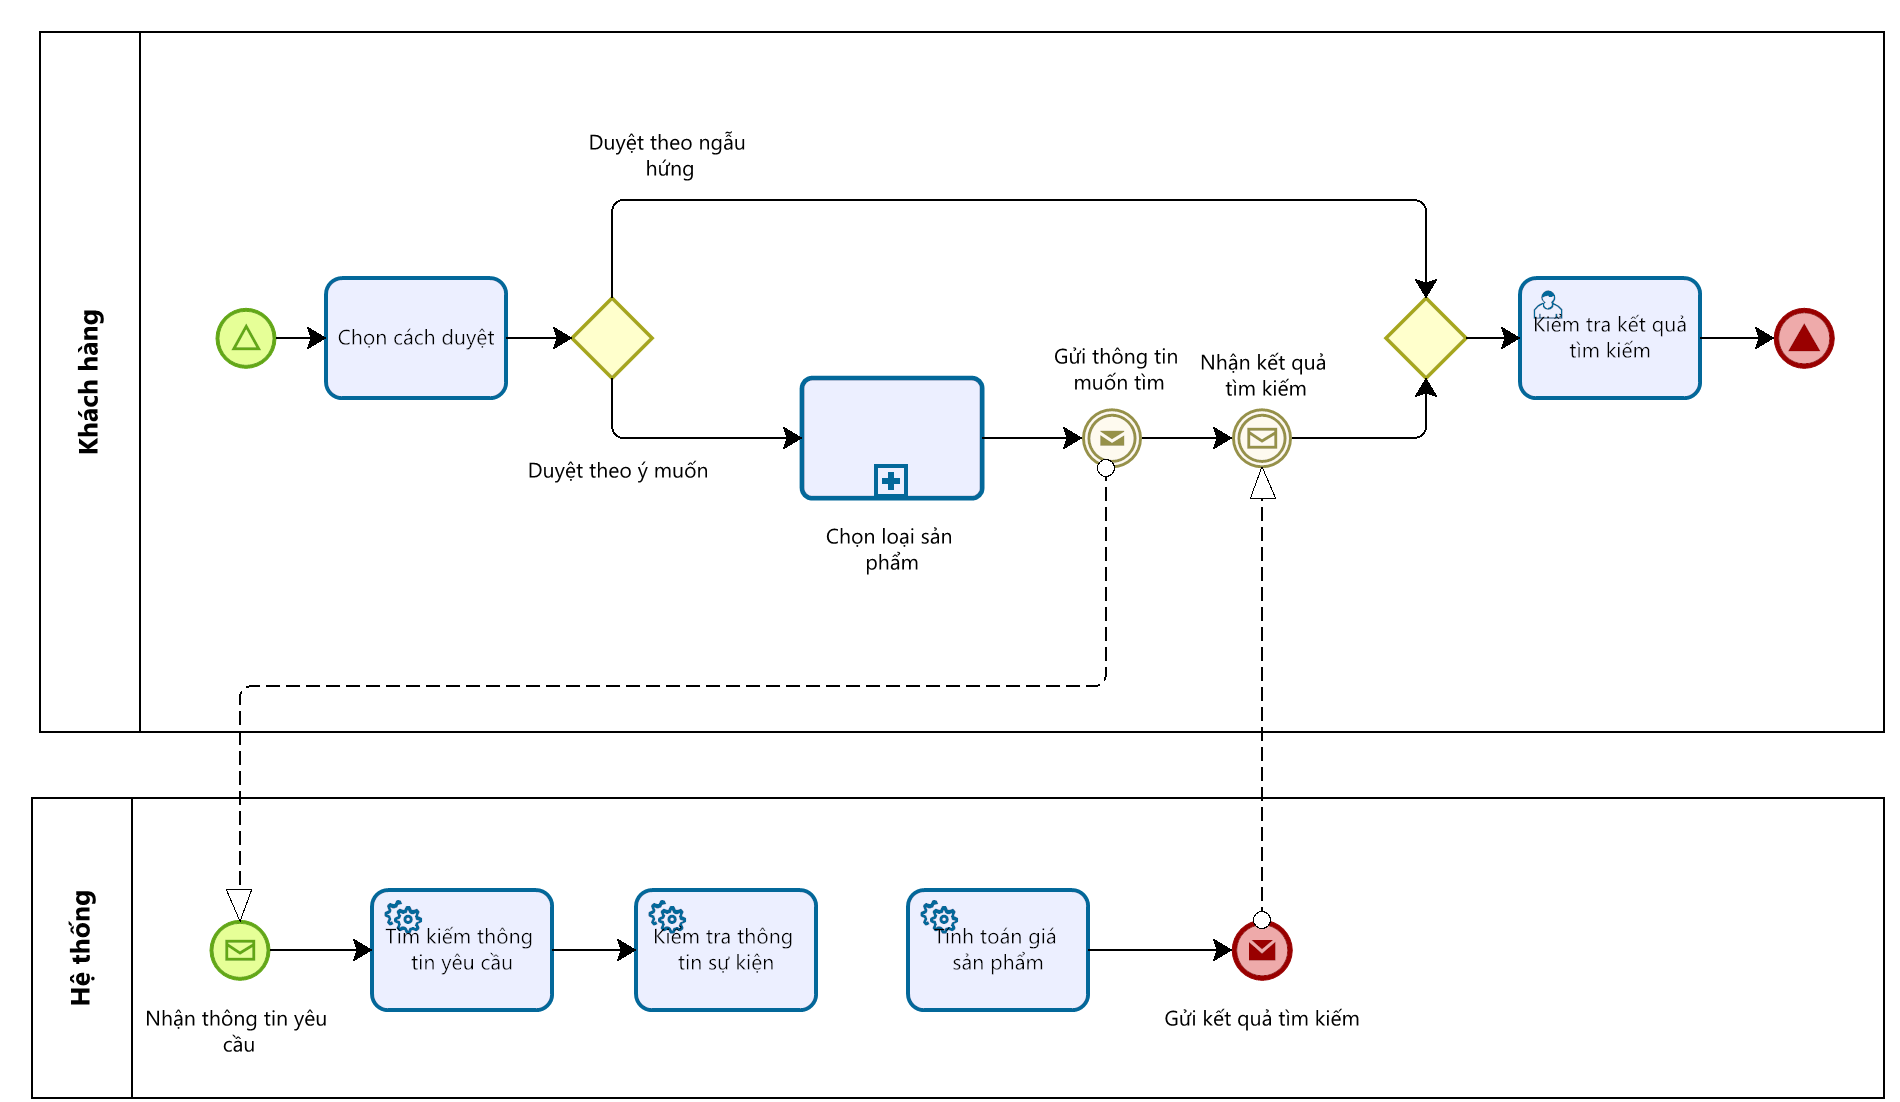
\includegraphics[width=13cm]{img/BPMN/customer_buy/customer_search_product.png}
    \newline
    \caption{Lược đồ BPMN cho quy trình con tìm kiếm sản phẩm}
\end{figure}
 
Đây là một quy trình con chứa quy trình tìm kiếm sản phẩm mà người dùng muốn tìm kiếm. Bắt đầu từ việc chọn cách duyệt bằng cách duyệt theo ngẫu hứng hay duyệt theo ý muốn. Khi người dũng duyệt theo ý muốn thì thực hiện quy trình con "Chọn loại sản phẩm" để chọn những loại sản phẩm theo ý muốn của khách hàng. Sau khi chọn loại sản phẩm thì hệ thống sẽ nhận thông tin và xử lý, sau đó phản hồi kết quả và người dùng kiểm tra kết quả tìm kiếm và kết thúc quy trình con này.
 
\begin{figure}[!htp]
    \centering
    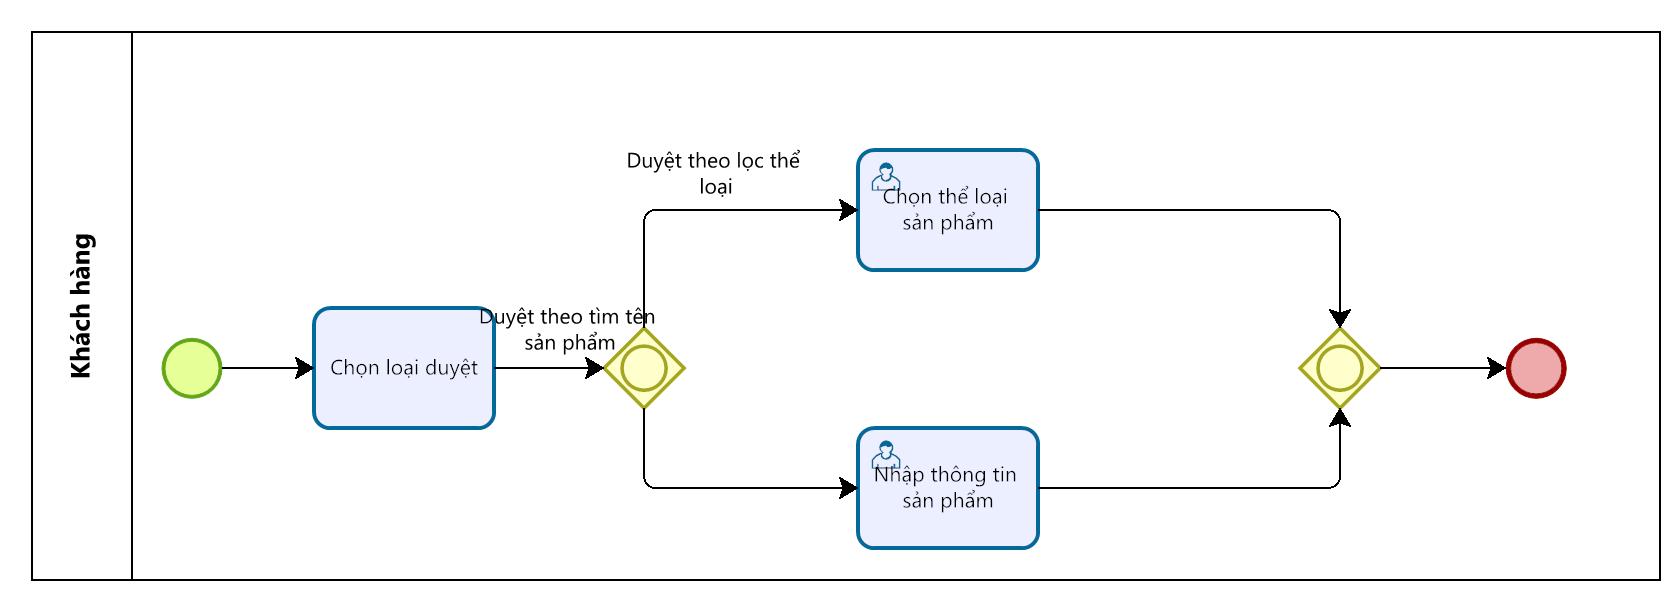
\includegraphics[width=12cm]{img/BPMN/customer_buy/customer_select_type.png}
    \newline
    \caption{Lược đồ BPMN cho quy trình con chọn loại sản phẩm mà khác hàng muốn tìm}
\end{figure}
 
Đây là một quy trình con chứa quy trình chọn loại sản phẩm mà người dùng muốn tìm kiếm. Bắt đầu từ việc chọn loại duyệt thì người dùng có thể chọn duyệt theo thể loại hoặc duyệt theo tên tìm kiếm hoặc duyệt theo sự kiện.
 
\newpage
 
\begin{figure}[!htp]
    \centering
    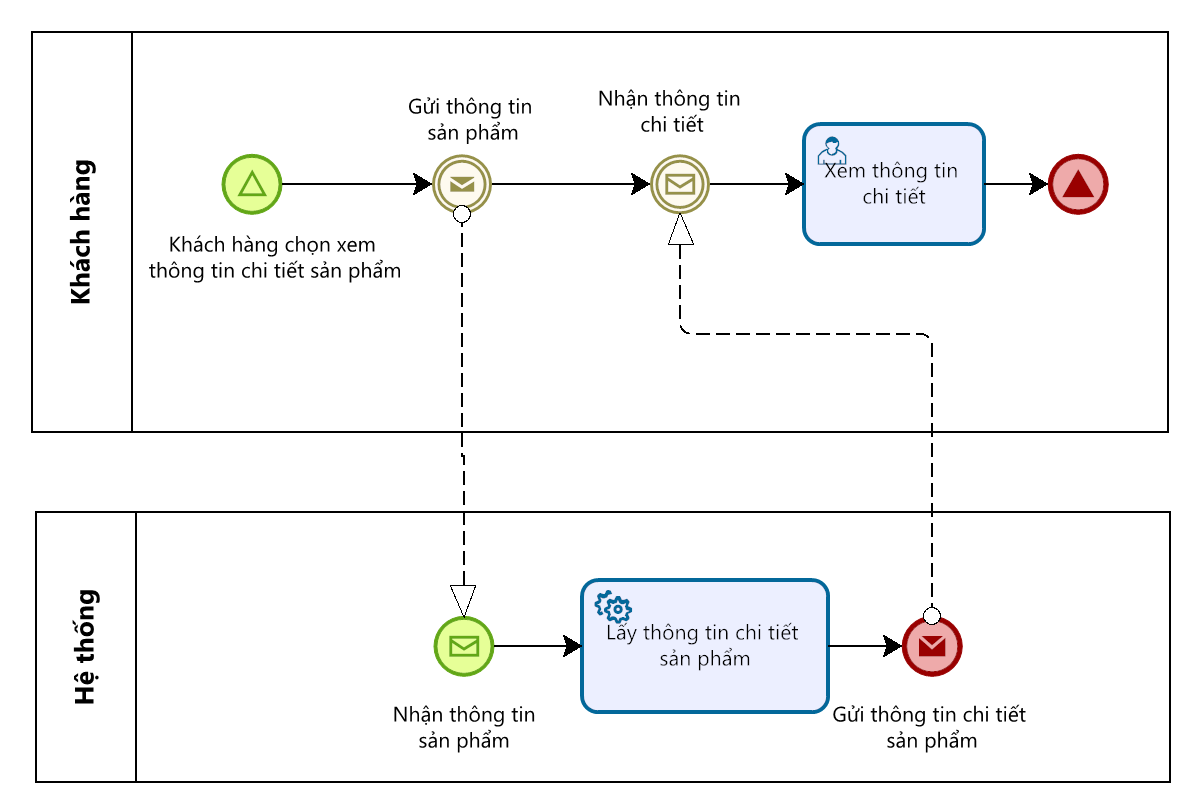
\includegraphics[width=10cm]{img/BPMN/customer_buy/customer_product_detail.png}
    \newline
    \caption{Lược đồ BPMN cho quy trình xem xét thông tin chi tiết của sản phẩm}
\end{figure}
 
Đây là một quy trình con chứa quy trình xem thông tin chi tiết của sản phẩm, sau khi khách hàng chọn sản phẩm muốn xem thông tin chi tiết thì hệ thống sẽ thực hiện lấy thông tin chi tiết sản phẩm từ cơ sở dữ liệu và phản hồi kết quả về cho khách hàng. Sau khi nhận được kết quả thì khách hàng xem thông tin chi tiết của sản phẩm và kết thúc quy trình.
 
 
 
\begin{figure}[!htp]
    \centering
    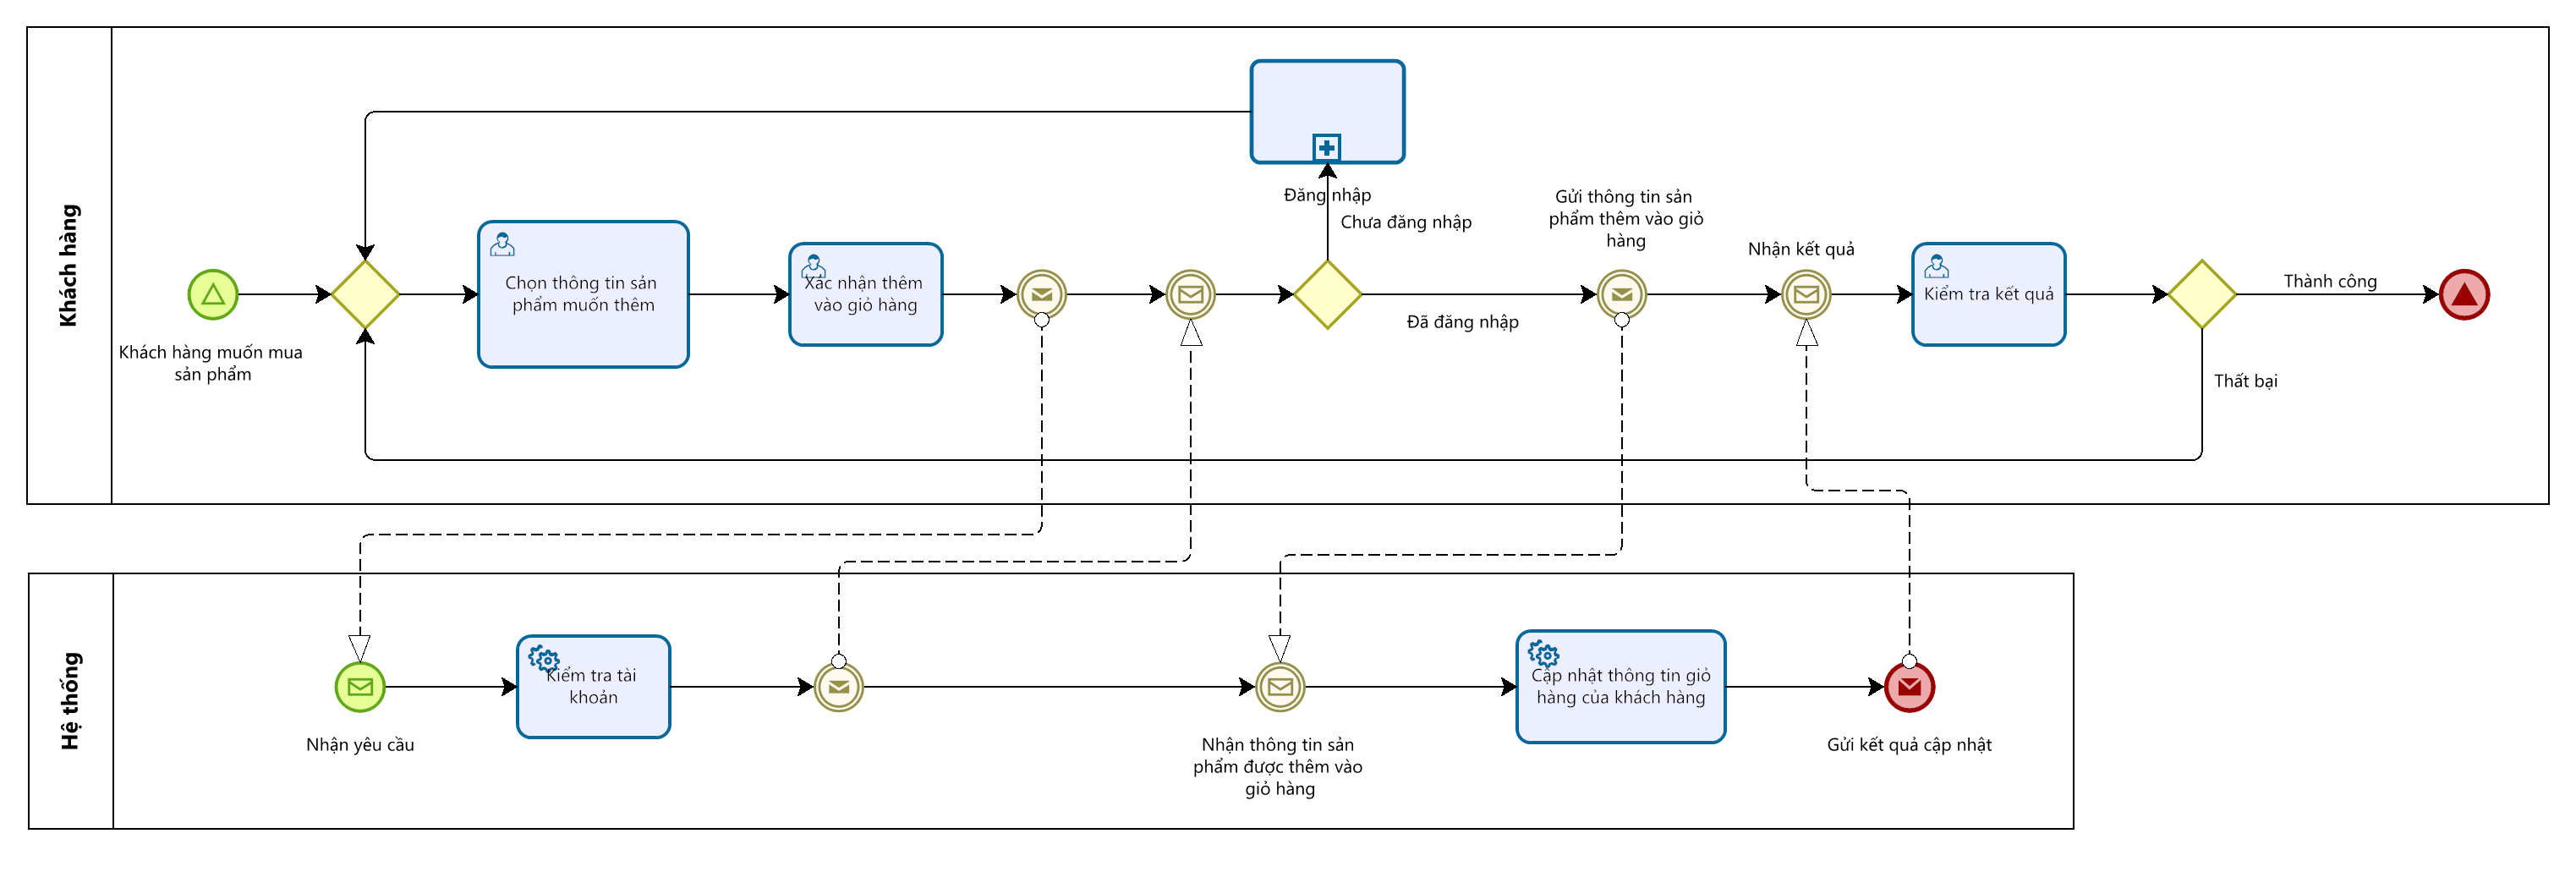
\includegraphics[width=17cm]{img/BPMN/customer_buy/customer_add_to_card.png}
    \newline
    \caption{Lược đồ BPMN cho quy trình thêm sản phẩm vào giỏ hàng}
\end{figure}
 
Đây là một quy trình con chứa quy trình thêm sản phẩm vào giỏ hàng, sau khi khách hàng xem thông tin chi tiết và muốn mua sản phẩm thì người dùng các thông tin sản phẩm mà khách hàng muốn thêm sau đó xác nhận thêm vào giỏ hàng. Thông tin sản phẩm khách hàng chọn thêm vào giỏ hàng được gửi đi và hệ thống thực hiện kiểm tra tài khoản khách hàng đã đăng nhập chưa, sau khi xác nhận được đã đăng nhập thì hệ thống kiểm tra thông tin và cập nhật thông tin sản phẩm vào giỏ hàng, sau đó gửi kết quả về phía khách hàng. Sau khi nhận được kết quả thì người dùng kiểm tra kết quả và kết thúc quy trình.
 
\newpage
 
\begin{figure}[!htp]
    \centering
    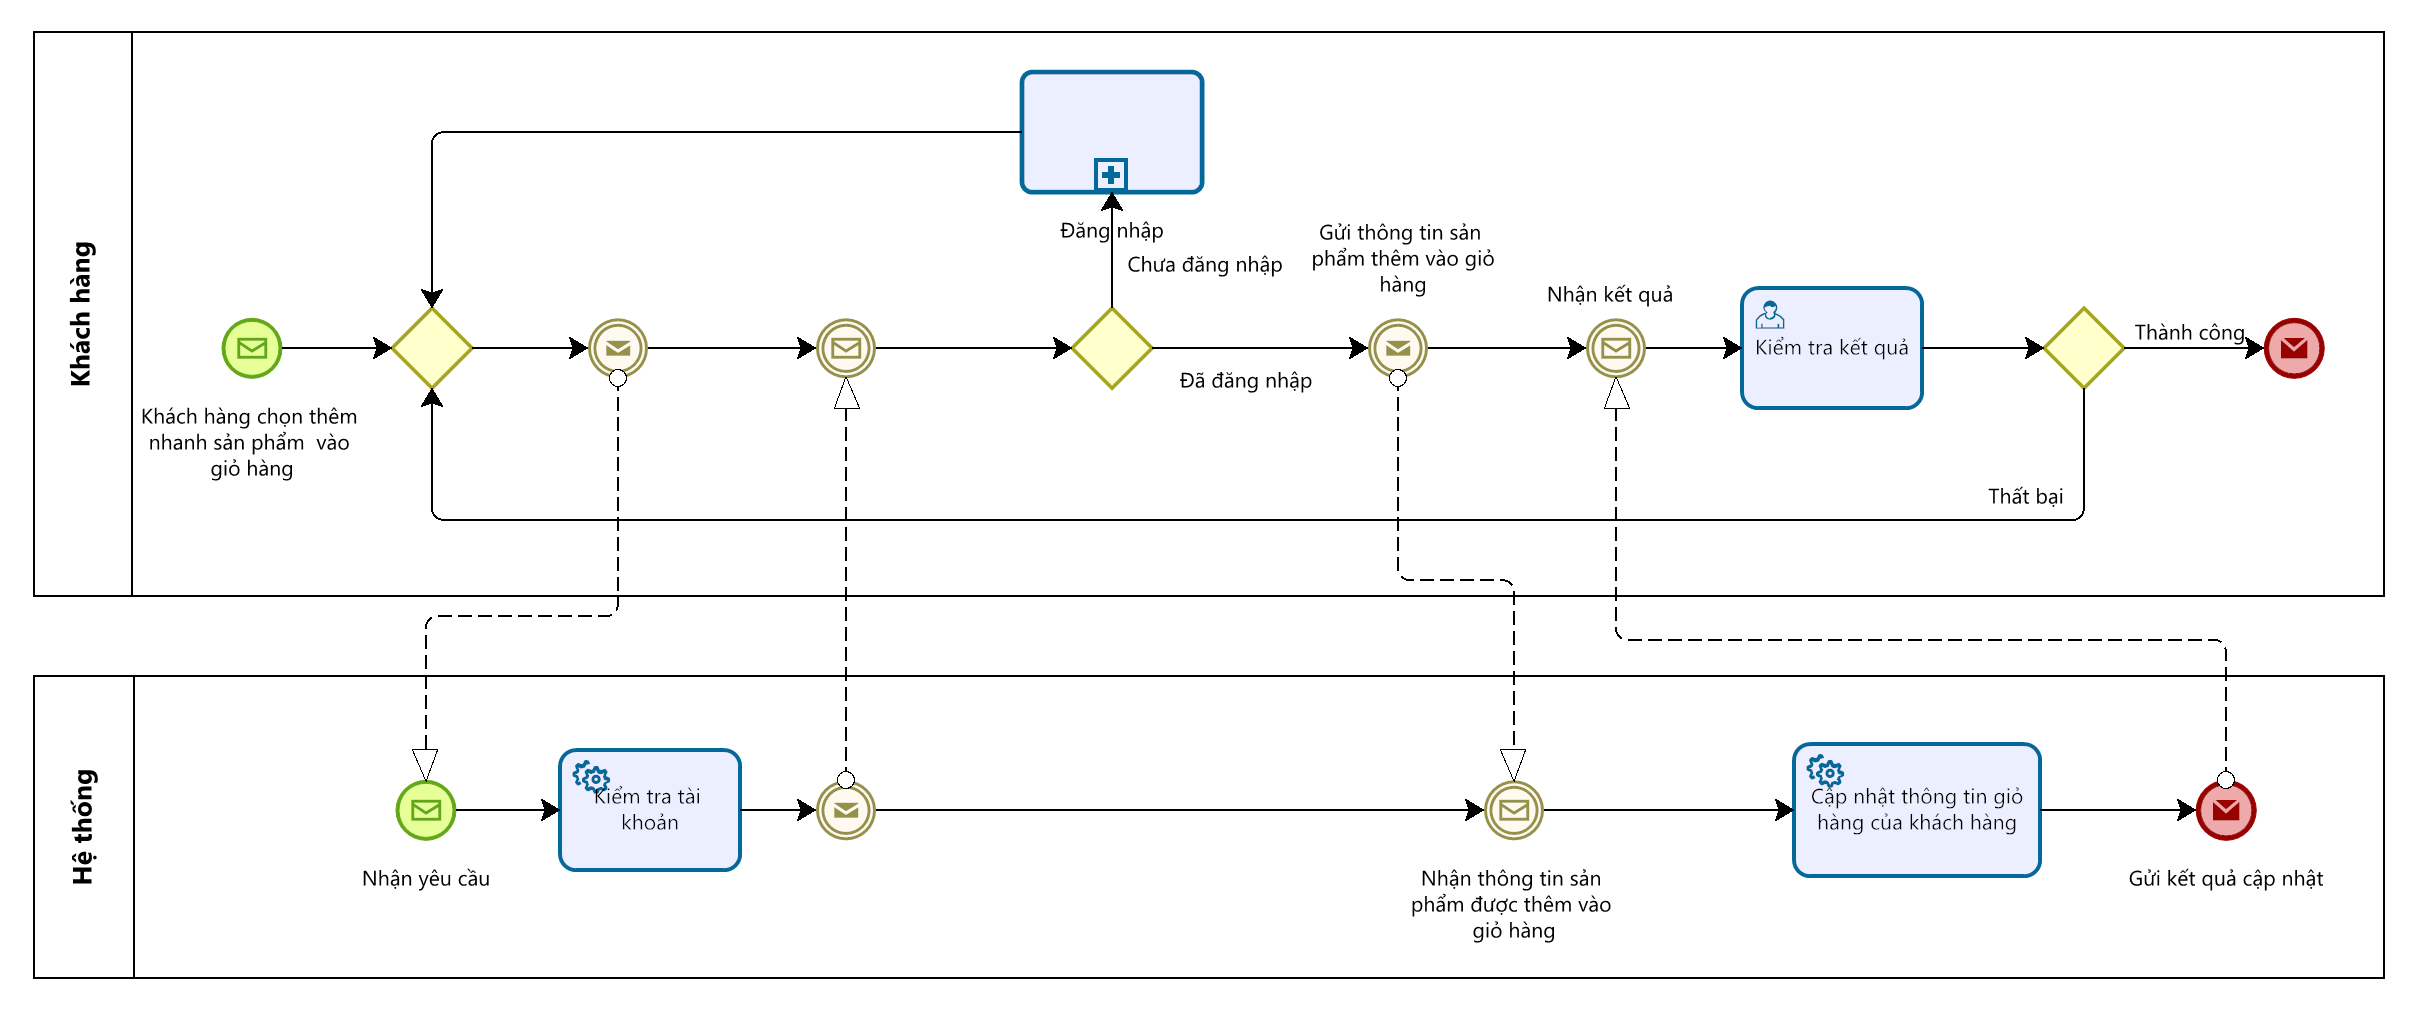
\includegraphics[width=16cm]{img/BPMN/customer_buy/customer_add_fast.png}
    \newline
    \caption{Lược đồ BPMN cho quy trình thêm nhanh sản phẩm vào giỏ hàng}
\end{figure}
 
Đây là một quy trình con chứa quy trình thêm nhanh sản phẩm vào giỏ hàng, sau khi khách hàng chọn thêm nhanh sản phẩm vào giỏ hàng. Thông tin sản phẩm khách hàng chọn thêm vào giỏ hàng được gửi đi và hệ thống thực hiện kiểm tra tài khoản khách hàng đã đăng nhập chưa, sau khi xác nhận được đã đăng nhập thì hệ thống kiểm tra thông tin và cập nhật thông tin sản phẩm vào giỏ hàng, sau đó gửi kết quả về phía khách hàng. Sau khi nhận được kết quả thì người dùng kiểm tra kết quả và kết thúc quy trình.
 
\begin{figure}[!htp]
    \centering
    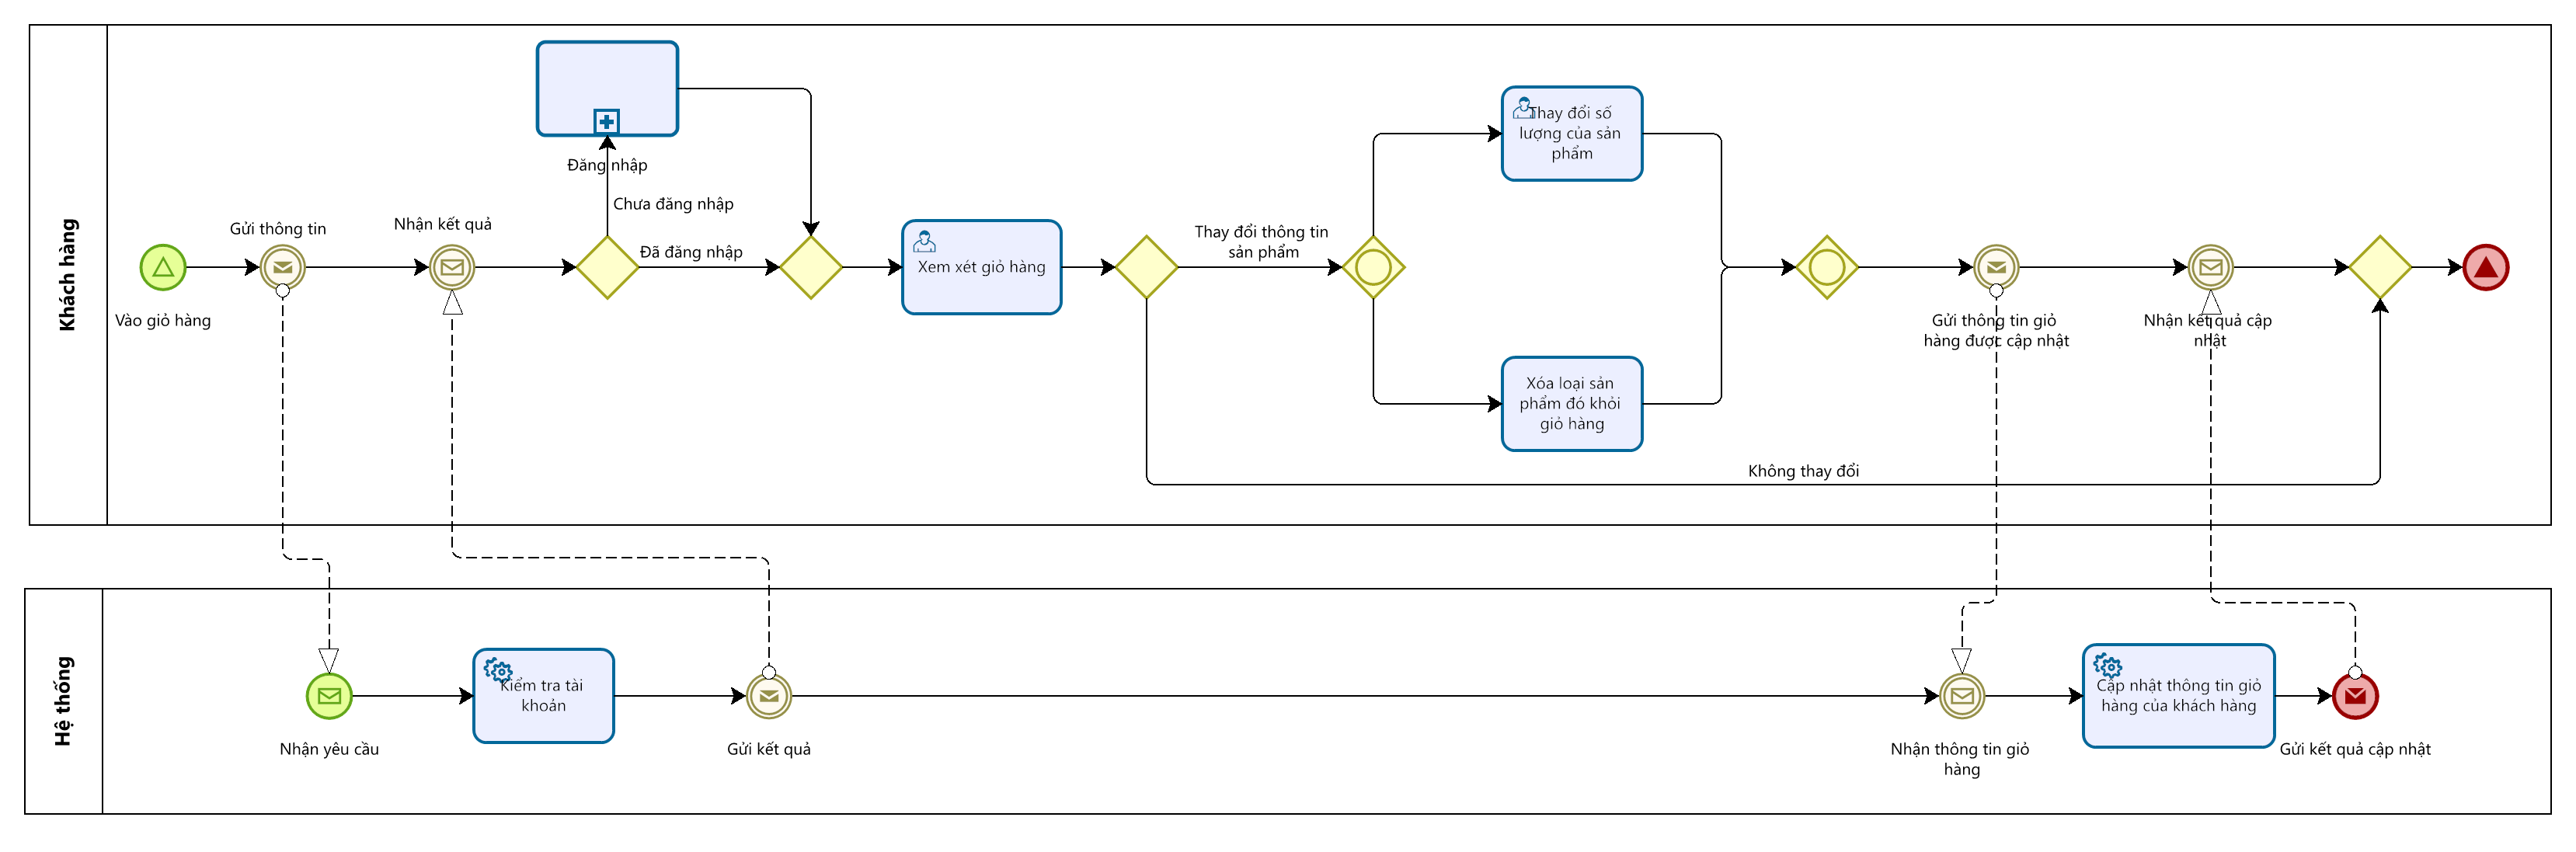
\includegraphics[width=17cm]{img/BPMN/customer_buy/customer_cart.png}
    \newline
    \caption{Lược đồ BPMN cho quy trình quản lý giỏ hàng}
\end{figure}
 
Đây là một quy trình con chứa quy trình quản lý giỏ hàng. Quy trình bắt đầu từ khi khách hàng chọn vào giỏ hàng. Hệ thống thực hiện kiểm tra tài khoản rồi sau đó truy xuất dữ liệu giỏ hàng của tài khoản khách hàng và phản hồi về lại cho khách hàng. Khách hàng thực thực hiện xem xét giỏ hàng và thực hiện thay đổi thông tin sản phẩm trong giỏ hàng bằng cách thay đổi thông tin sản phẩm hay xóa sản phẩm khỏi giỏ hàng, hệ thống nhận thông tin thay đổi sau đó kiểm tra thông tin và cập nhật thông tin giỏ hàng rồi trả về kết quả, khách hàng nhận kết quả và kết thúc quy trình.
 
\newpage
 
\begin{figure}[!htp]
    \centering
    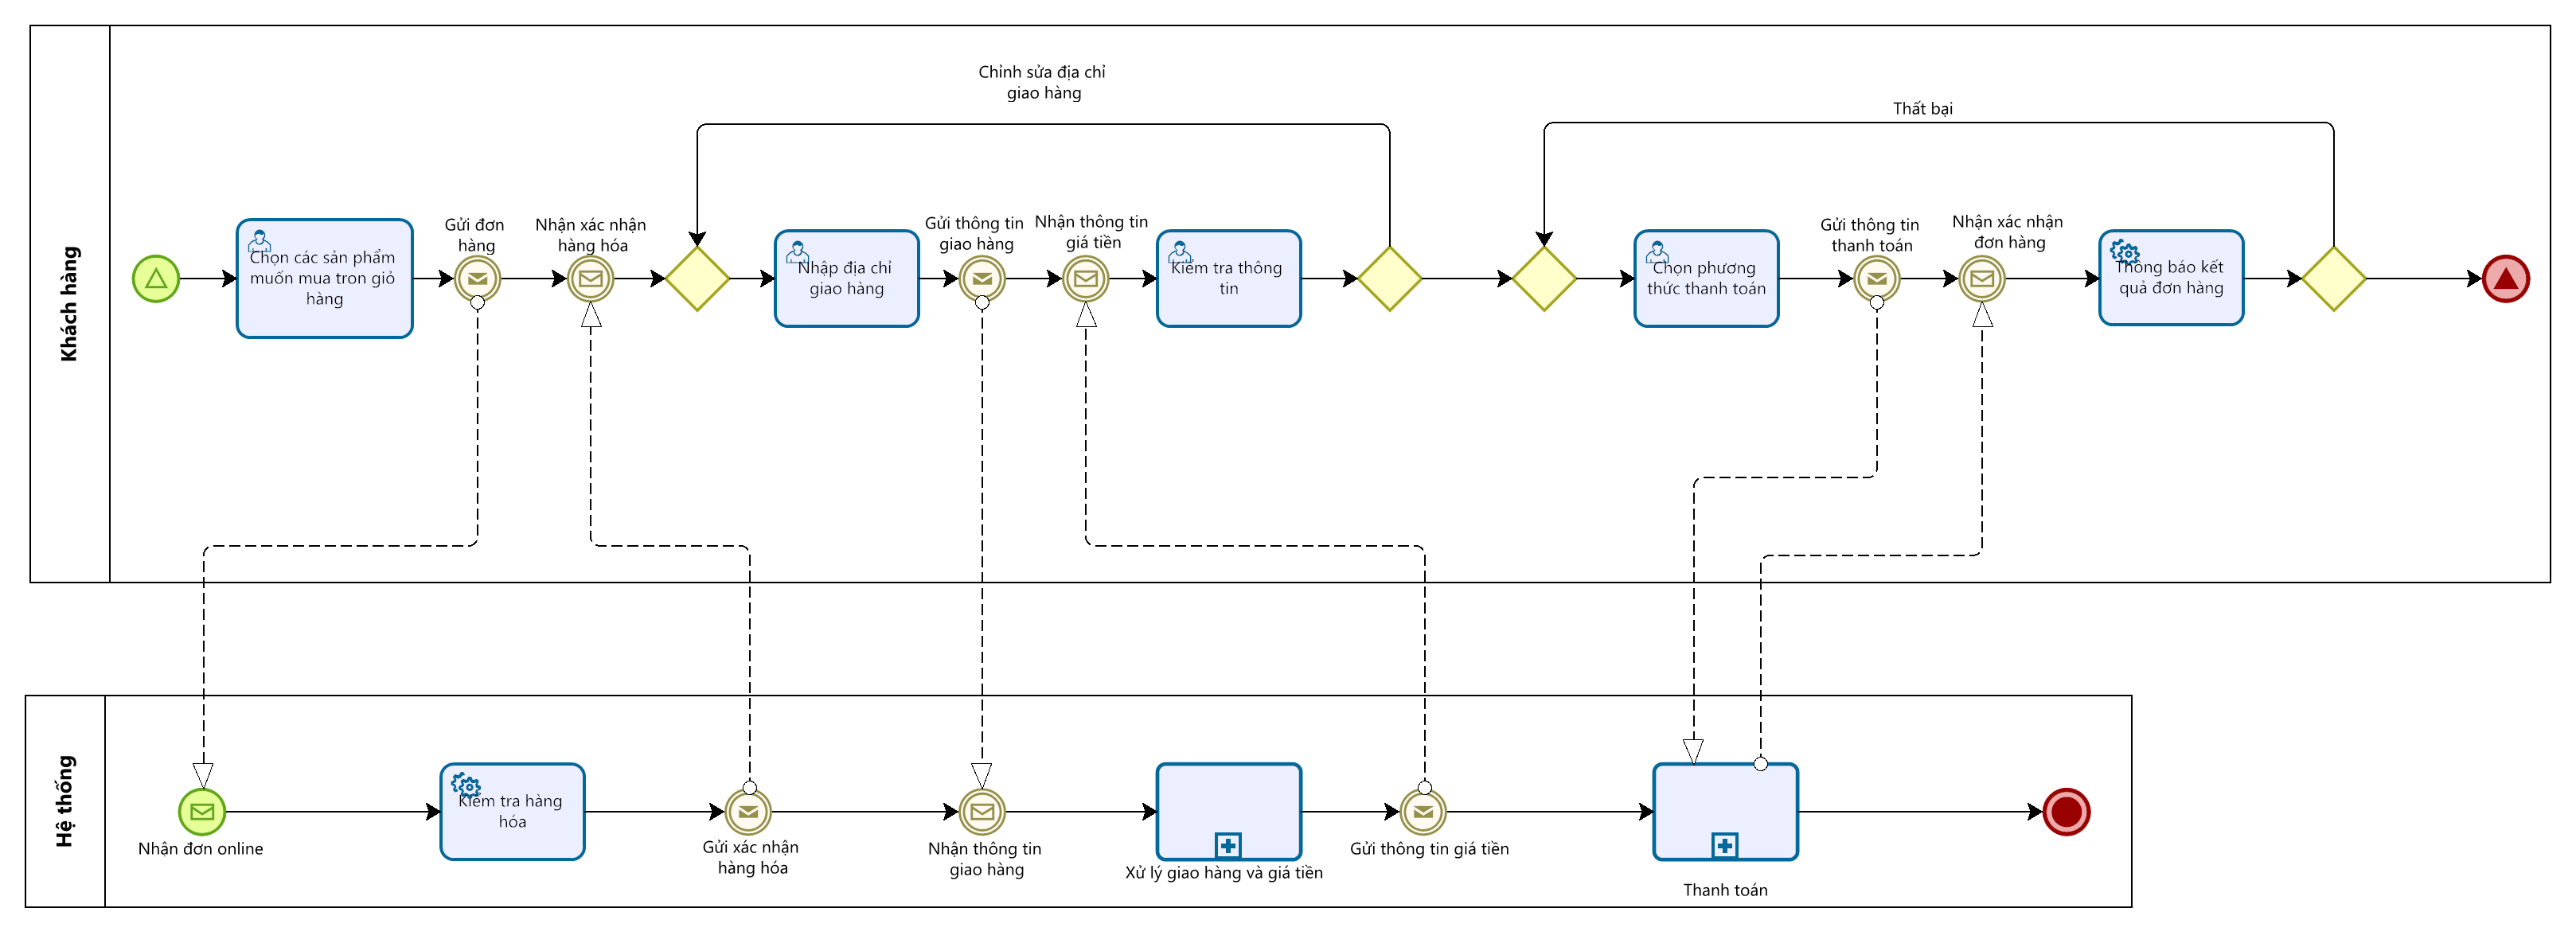
\includegraphics[width=17cm]{img/BPMN/customer_buy/customer_buy_order.png}
    \newline
    \caption{Lược đồ BPMN cho quy trình mua hàng}
\end{figure}
 
Đây là một quy trình con chứa quy trình đặt mua hàng của khách hàng. Khách hàng chọn các sản phẩm trong giỏ hàng mà bản thân muốn mua và chọn "Đặt hàng". Hệ thống thực hiện kiểm tra hàng hóa và phản hồi về lại cho khách hàng. Sau khi chọn "Đặt hàng" và nhận kết quả xác nhận hàng hóa, khách hàng thực thực hiện nhập địa chỉ giao hàng, hệ thống sẽ thực hiện xử lý giao hàng và giá tiền để tính tổng hóa hơn cho khách hàng. Khách hàng thực hiện kiểm tra thông tin sau khi nhận lại thông tin giá tiền, nếu chưa chính xác về địa chỉ gia hàng thì quay lại nhập địa chỉ giao hàng, nếu đã chính xác thì thực hiện chọn phương thức thanh toán và chọn "Thanh toán". Hệ thống kiểm tra thông tin thanh toán mà người dùng chọn sau đó thực hiện quy trình "Thanh toán", sau khi kết thúc quy trình thanh toán thì hệ thống phản hồi và hiển thị thông báo kết quả đơn hàng, nếu thành công thì kết thúc quy trình, nếu thất bại thì khách hàng quay lại chọn phương thức thanh toán phù hợp.
 
\begin{figure}[!htp]
    \centering
    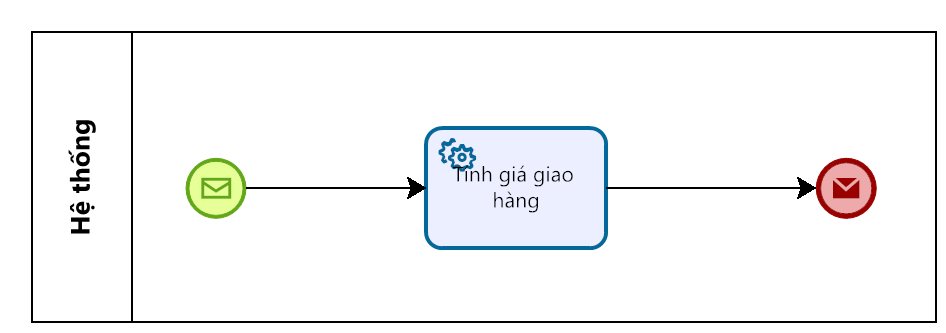
\includegraphics[width=5in]{img/BPMN/customer_buy/customer_calc_fee.png}
    \newline
    \caption{Lược đồ BPMN cho quy trình tính toán chi phí đơn hàng}
\end{figure}
 
Đây là một quy trình con chứa quy trình tính toán chi phí đơn hàng. Hệ thống thực hiện kiểm tra kho để tạo đơn hàng vận chuyển, nếu không có kho nào đủ hàng cho khách hàng thì cần thực hiện tính toán trao đổi kho và gửi thông tin trao đổi hàng cho kho. Sau khi thực hiện tính toán kho thì thực hiện tính toán giá giao hàng và tính tổng tiền của đơn hàng.
 
\begin{figure}[!htp]
    \centering
    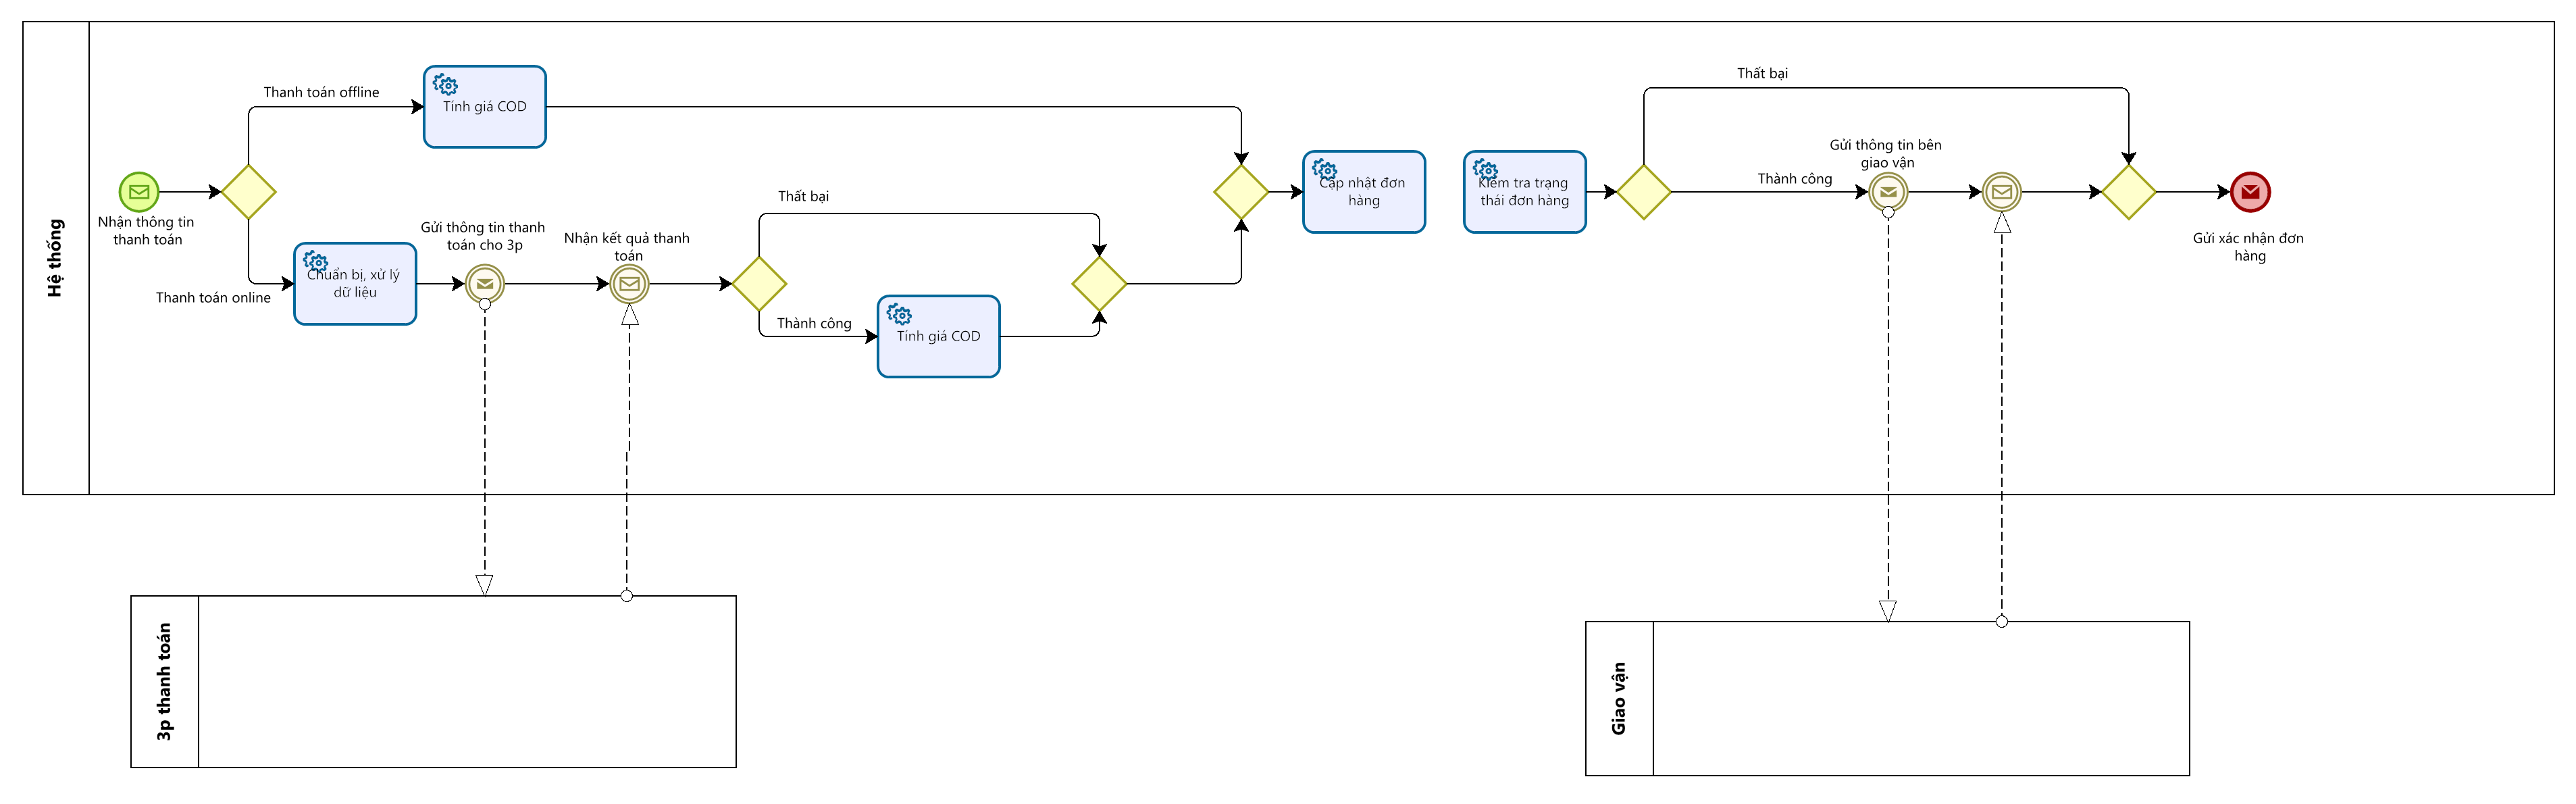
\includegraphics[width=15cm]{img/BPMN/customer_buy/customer_payment.png}
    \newline
    \caption{Lược đồ BPMN cho quy trình thanh toán đơn hàng}
\end{figure}
 
Đây là một quy trình con chứa quy trình thanh toán đơn hàng. Quy trình bắt đầu từ sự kiện nhận thông tin thanh toán, nếu thanh toán trực tiếp khi nhận hàng thì thực hiện cập nhật đơn hàng. Nếu phương thức thanh toán là trực tuyến thì hệ thống thực hiện gửi thông tin thanh toán cho bên thứ ba tương ứng với bên mà người dùng chọn, sau đó chờ bên thứ ba trả về kết quả thanh toán. Sau khi nhận được kết quả từ bên thứ ba thì thông báo kết quả với người dùng, nếu thanh toán thành công thì thực hiện cập nhật đơn hàng vào hệ thống, khi cập nhật đơn hàng thành công thì thực hiện gửi thông tin vận chuyển đến dịch vụ vận chuyển của bên thứ ba và kết thúc quy trình.


\subsection{Quản lý sự kiện}

\subsubsection{Thêm sự kiện}

\begin{figure}[!htp]
	\centering
	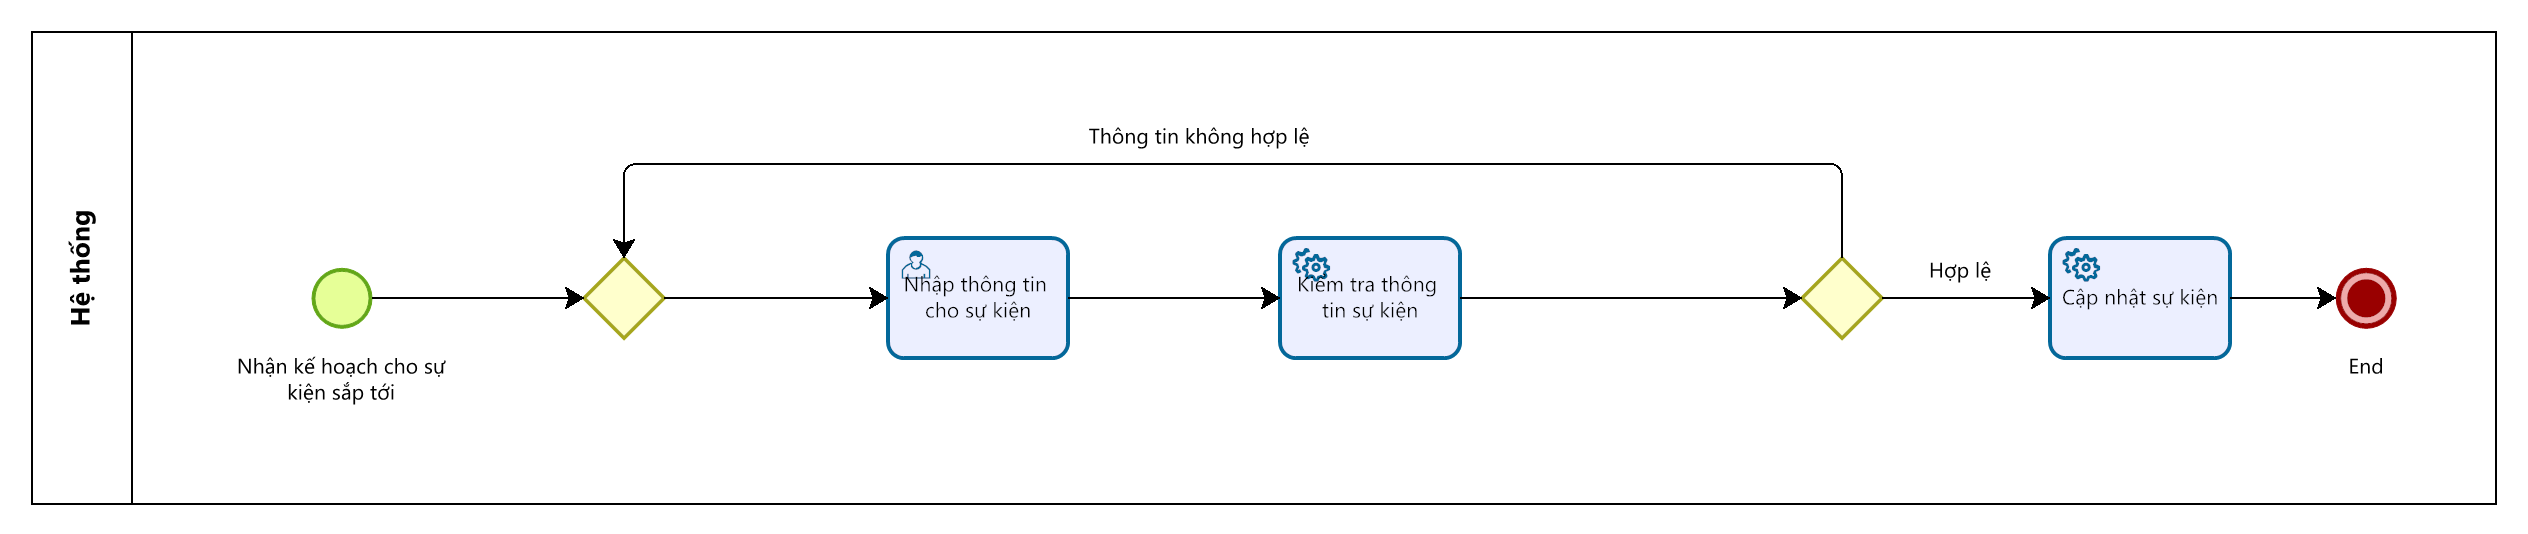
\includegraphics[width=14cm]{img/BPMN/event/add_event.png}
	\newline
	\caption{Lược đồ BPMN cho quy trình thêm sự kiện}
\end{figure}

Quy trình được bắt đầu bởi sự kiện nhận thông tin cho sự kiện sắp tới, sau khi nhận được thông tin sự kiện mới thì quản trị viên nhập thông tin cho sự kiện và xác nhận tạo sự kiện. Sau khi thông tin sự kiện mới được gửi đi thì hệ thống sẽ kiểm tra thông tin sự kiện có hợp lệ hay không, nếu hợp lệ thì cập nhật sự kiện mới vào hệ thống và kết thúc quy trình, nếu không hợp lệ thì quản trị viên cần quay lại task nhập lại thông tin cho sự kiện.

\subsubsection{Sửa sự kiện}

\begin{figure}[!htp]
	\centering
	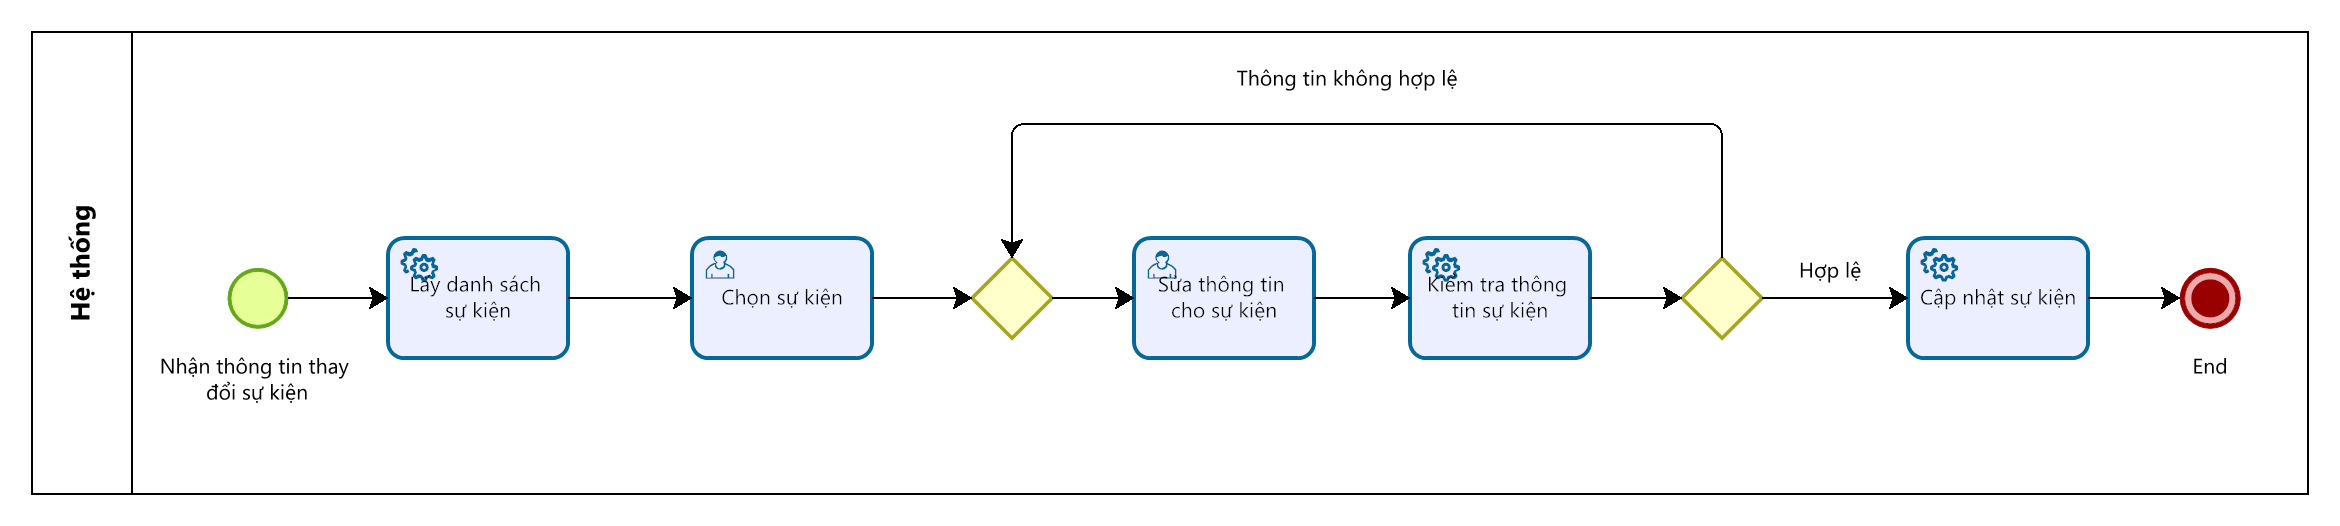
\includegraphics[width=14cm]{img/BPMN/event/edit_event.png}
	\newline
	\caption{Lược đồ BPMN cho quy trình chỉnh sửa sự kiện}
\end{figure}

Quy trình được bắt đầu bởi sự kiện nhận thông tin thay đổi sự kiện, sau khi nhận được thông tin sự kiện cần cập nhật thì quản trị viên chọn sự cần cần sửa, sau đó nhập thông tin cho sự kiện và xác nhận cập nhật sự kiện. Sau khi thông tin cập nhật sự kiện được gửi đi thì hệ thống sẽ kiểm tra thông tin sự kiện có hợp lệ hay không, nếu hợp lệ thì cập nhật lại sự kiện vào hệ thống và kết thúc quy trình, nếu không hợp lệ thì quản trị viên cần quay lại task nhập lại thông tin cho sự kiện.

\subsubsection{Xóa sự kiện}

\begin{figure}[!htp]
	\centering
	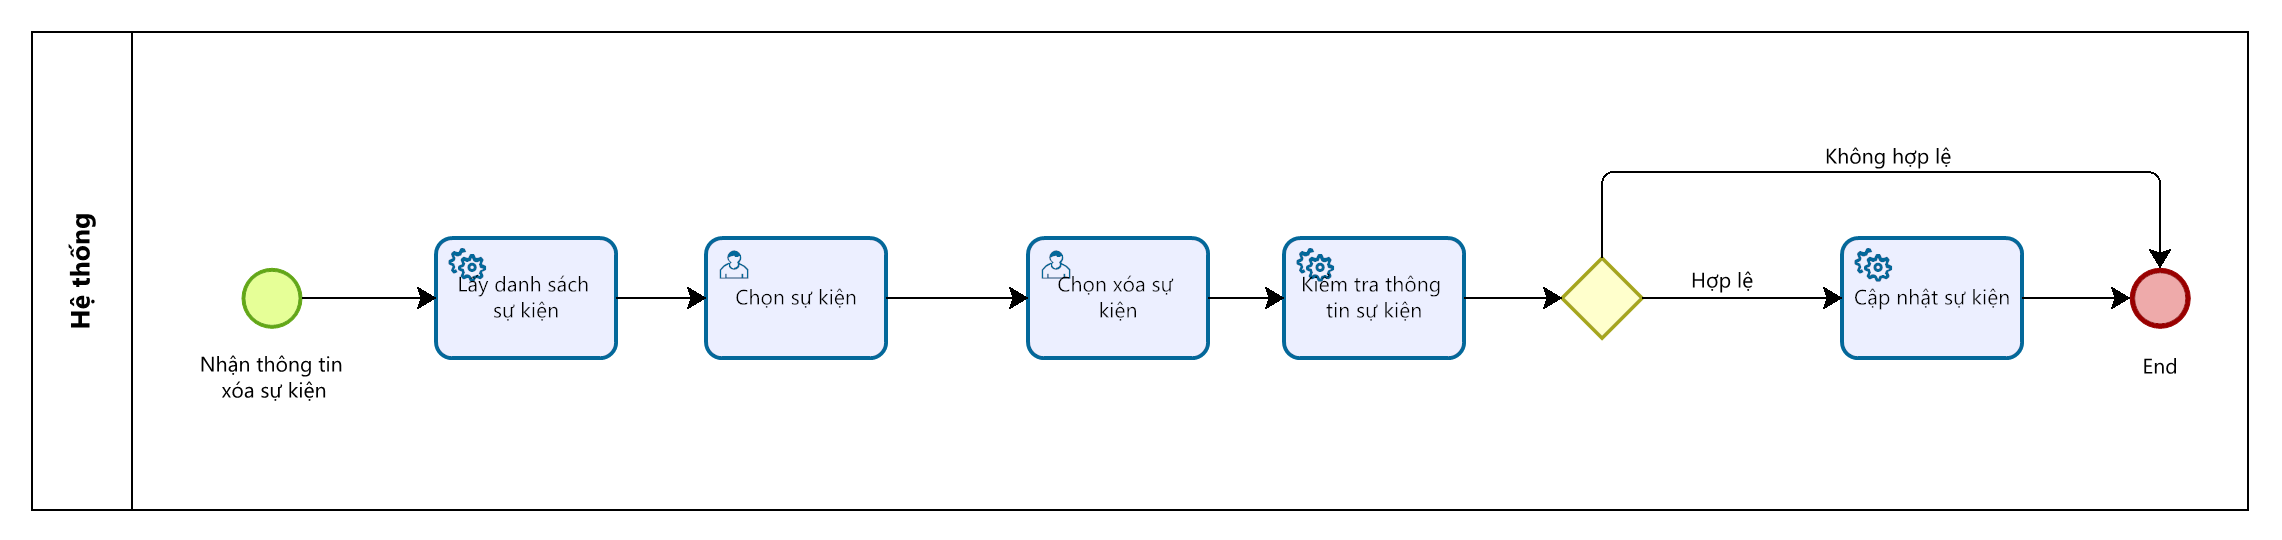
\includegraphics[width=14cm]{img/BPMN/event/delete_event.png}
	\newline
	\caption{Lược đồ BPMN cho quy trình xóa sự kiện}
\end{figure}

Quy trình được bắt đầu bởi sự kiện nhận thông tin xóa sự kiện, sau khi nhận được thông tin sự kiện cần cập nhật thì quản trị viên chọn sự cần cần xóa và chọn xóa sự kiện. Sau khi thông tin sự kiện cần xóa được gửi đi thì hệ thống sẽ kiểm tra thông tin sự kiện có hợp lệ hay không, nếu hợp lệ thì cập nhật xóa sự kiện khỏi hệ thống và kết thúc quy trình, nếu không hợp lệ thì thông báo thất bại và kết thúc quy trình.


\subsection{Khách hàng mua hàng trực tiếp}
\begin{figure}[!htp]
	\centering
	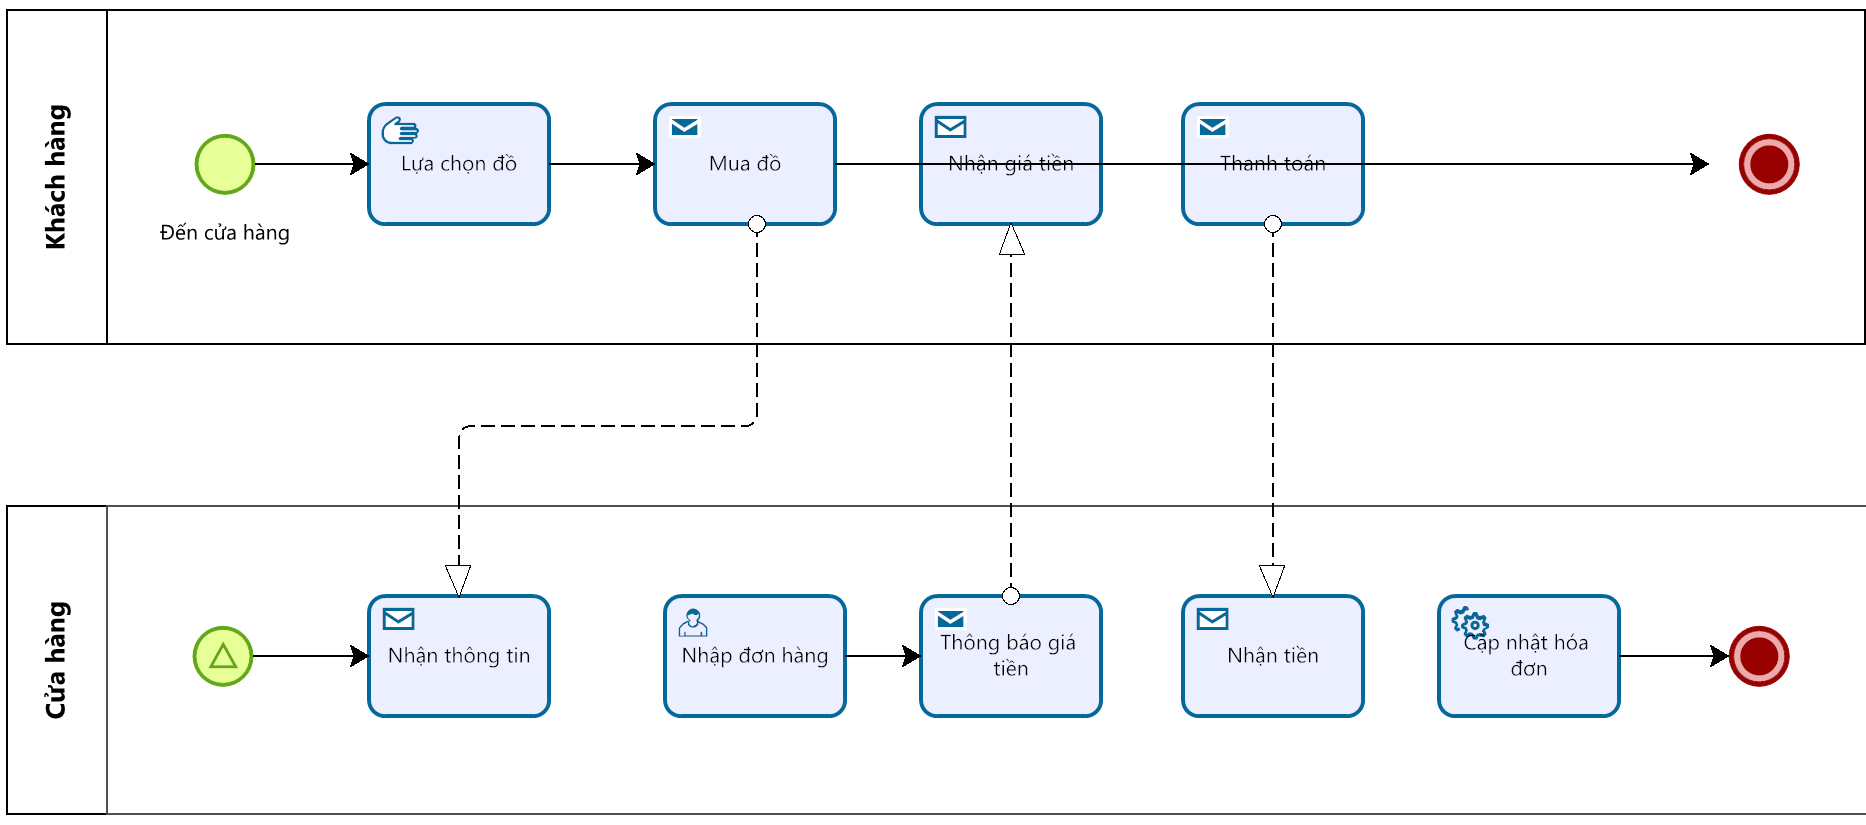
\includegraphics[width=13cm]{img/BPMN/Hien/Customer_buyOffline.png}
	\newline
	\caption{Lược đồ BPMN cho quy trình khách hàng mua hàng trực tiếp}
\end{figure}

Khách hàng sau khi đến cửa hàng sẽ thực hiện chọn sản phẩm và thông báo cho nhân viên sản phẩm của mình. Nhân viên thực hiện nhập đơn hàng và báo giá cho khách hàng. Khách hàng nhận thông tin và thực hiện thanh toán. Nhân viên nhân tiền và cập nhật hóa đơn trên hệ thống

\subsection{Đăng nhập}
\begin{figure}[!htp]
	\centering
	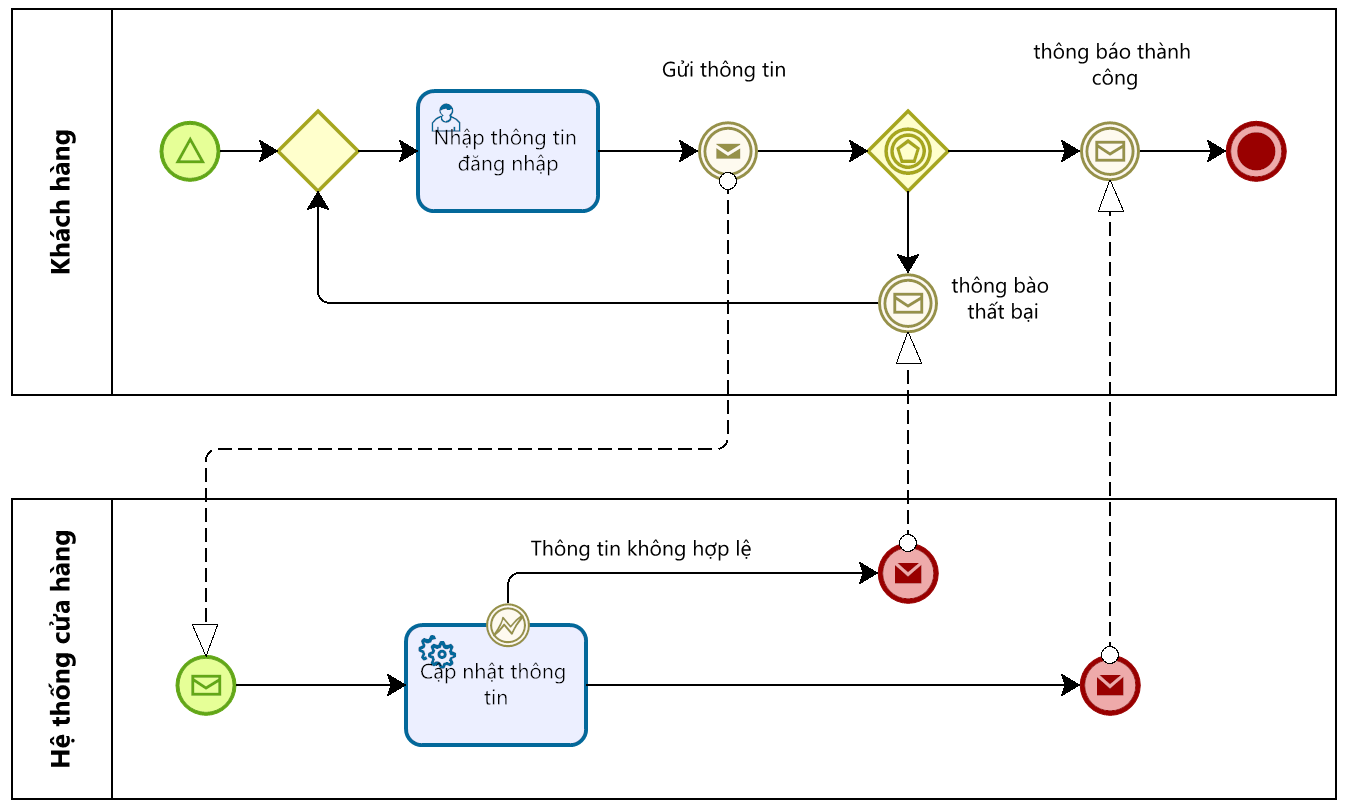
\includegraphics[width=10cm]{img/BPMN/Hien/Customer_login.png}
	\newline
	\caption{Lược đồ BPMN cho quy trình đăng nhập}
\end{figure}

Người dùng truy cập hệ thống nhập thông tin đăng nhập và chọn đăng nhập. Hệ thống thực hiện kiểm tra thông tin và trả thông báo thành công hoặc thất bại. Nếu thất bại sẽ yêu cầu người dùng đăng nhập lại

\newpage

\subsection{Đăng ký tài khoản}
\begin{figure}[!htp]
	\centering
	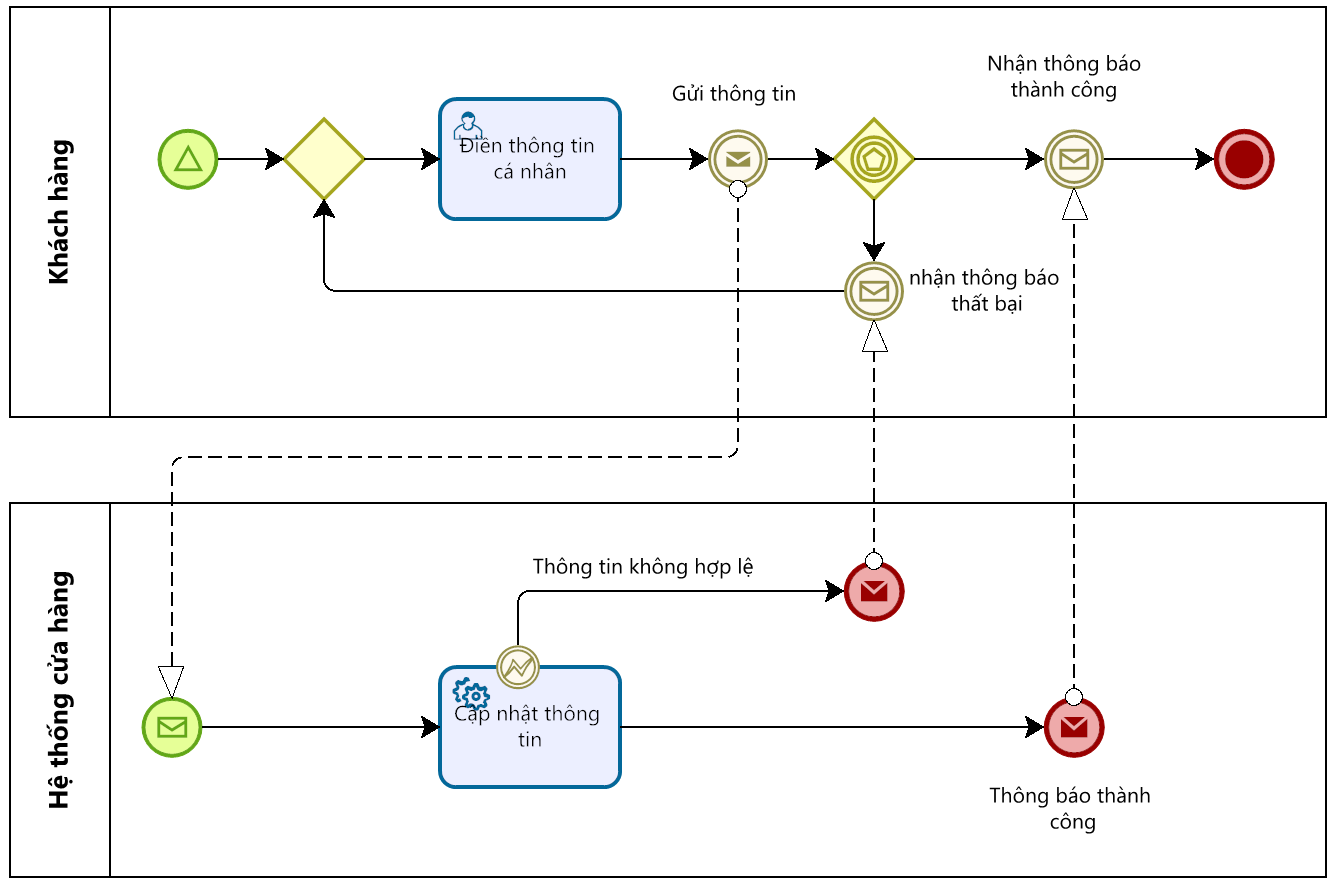
\includegraphics[width=10cm]{img/BPMN/Hien/Customer_register.png}
	\newline
	\caption{Lược đồ BPMN cho quy trình đăng ký tài khoản mới}
\end{figure}

Người dùng nhập thông tin cá nhân và chọn đăng ký. Hệ thống nhận thông tin và cập nhật. Hệ thống thông báo thành công nếu thành công và thông báo thất bại nếu thông tin không hợp lệ


\subsection{Làm mới mật khẩu}
\begin{figure}[!htp]
	\centering
	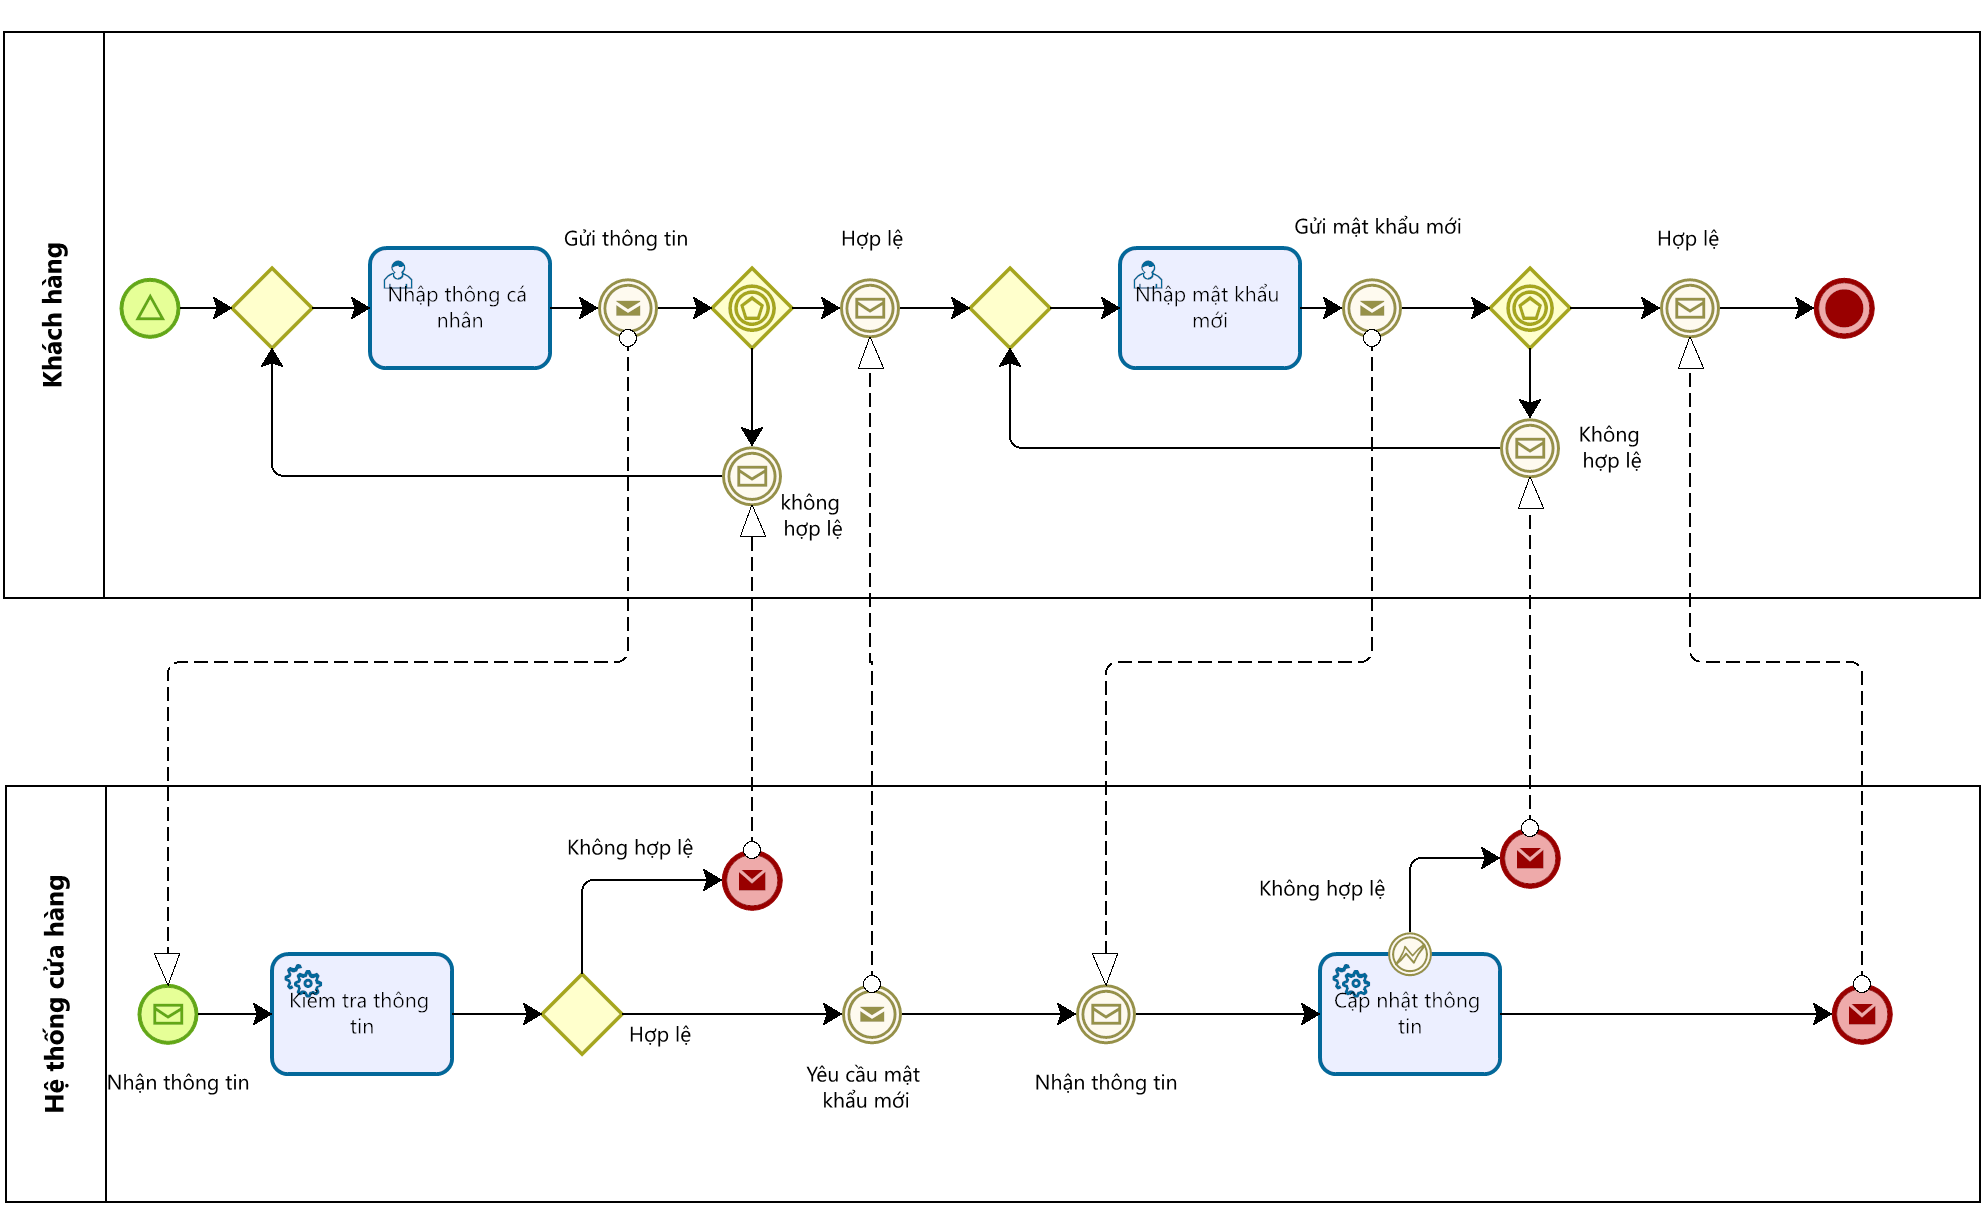
\includegraphics[width=14cm]{img/BPMN/Hien/Customer_resetPassword.png}
	\newline
	\caption{Lược đồ BPMN cho quy trình làm mới mật khẩu}
\end{figure}

Người dùng nhập thông tin cá nhân và gửi. Hệ thống kiểm tra thông tin, nếu hợp lệ sẽ yêu cầu mật khẩu mới từ người dùng; ngược lại sẽ yêu cầu người dùng nhập lại thông tin. Sau khi người dùng nhập mật khẩu mới và gửi, hệ thống sẽ cập nhật thông tin và gửi thông báo thành công, nếu mật khẩu không hợp lệ sẽ yêu cầu người dùng nhập lại.
\newpage

\subsection{Quản lý chi nhánh}
\begin{figure}[!htp]
	\centering
	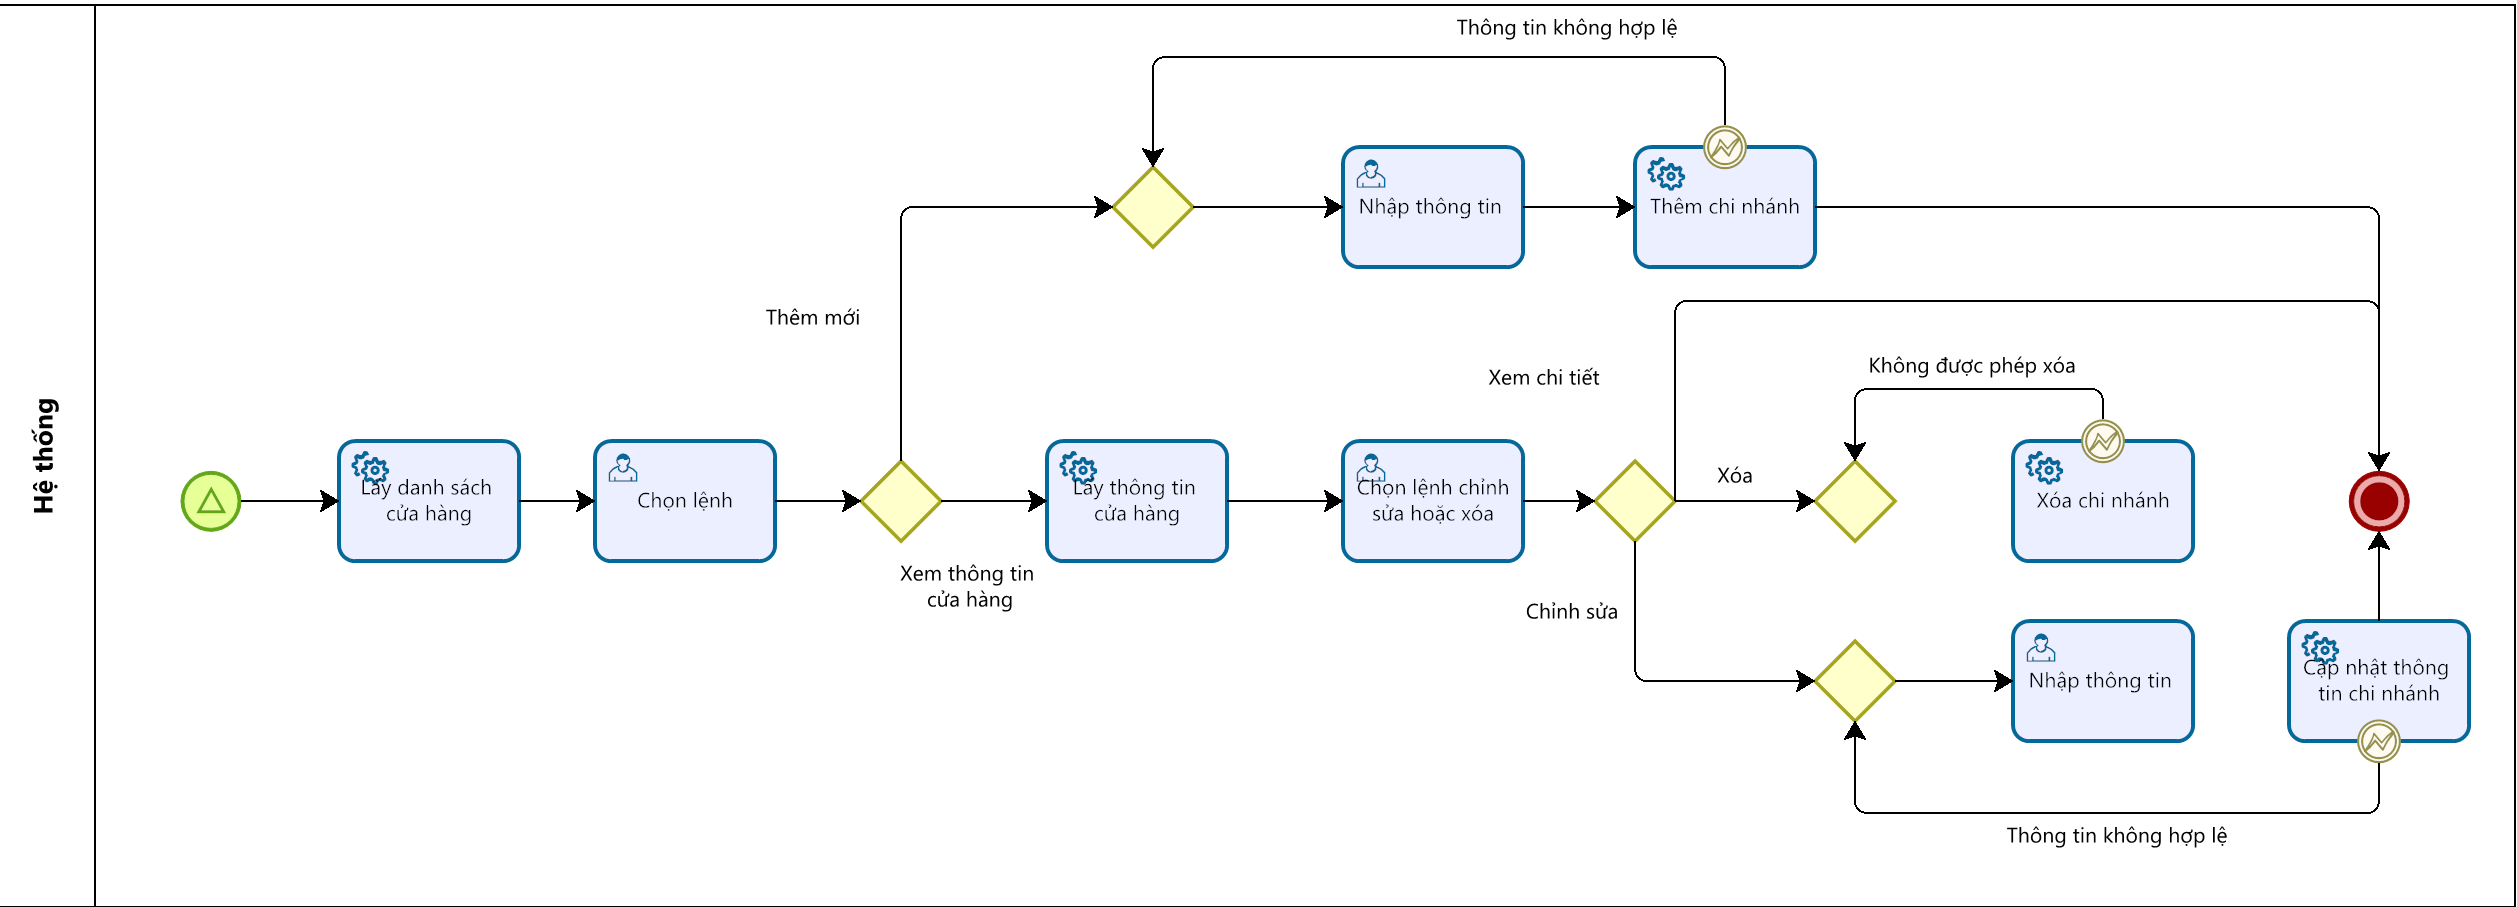
\includegraphics[width=16cm]{img/BPMN/Hien/Branch_management.png}
	\newline
	\caption{Lược đồ BPMN cho quy trình quản lý chi nhánh}
\end{figure}

Khi quản trị viên truy cập, hệ thống sẽ lấy danh sách chi nhánh. Quản trị viên thực hiện thêm mới hoặc xem thông tin chi nhánh. Nêu thêm mới, quản trị viên sẽ nhập thông tin chi nhánh mới và cập nhật hệ thống. Nâu có thông tin không hợp lệ, hệ thống sẽ yêu cầu nhập lại thông tin. Nếu xem thông chi nhánh, hệ thống sẽ lấy thông tin chi tiết của chi nhánh đó. Quản trị viên có thể chỉ xem thông tin chi nhánh, chỉnh sửa thông tin hoặc xóa chi nhánh. Nếu chọn xóa, hệ thống sẽ kiểm tra và xóa nếu hợp lệ, ngược lại sẽ hiện thông tin chi tiết chi nhánh. Nếu chọn chỉnh sửa, hệ thống yêu cầu nhập thông tin sẽ kiểm tra thông tin nếu hợp lệ sẽ cập nhật thông tin, ngược lại sẽ yêu cầu nhập lại thông tin


\subsection{Quản lý nhân viên}
\begin{figure}[!htp]
	\centering
	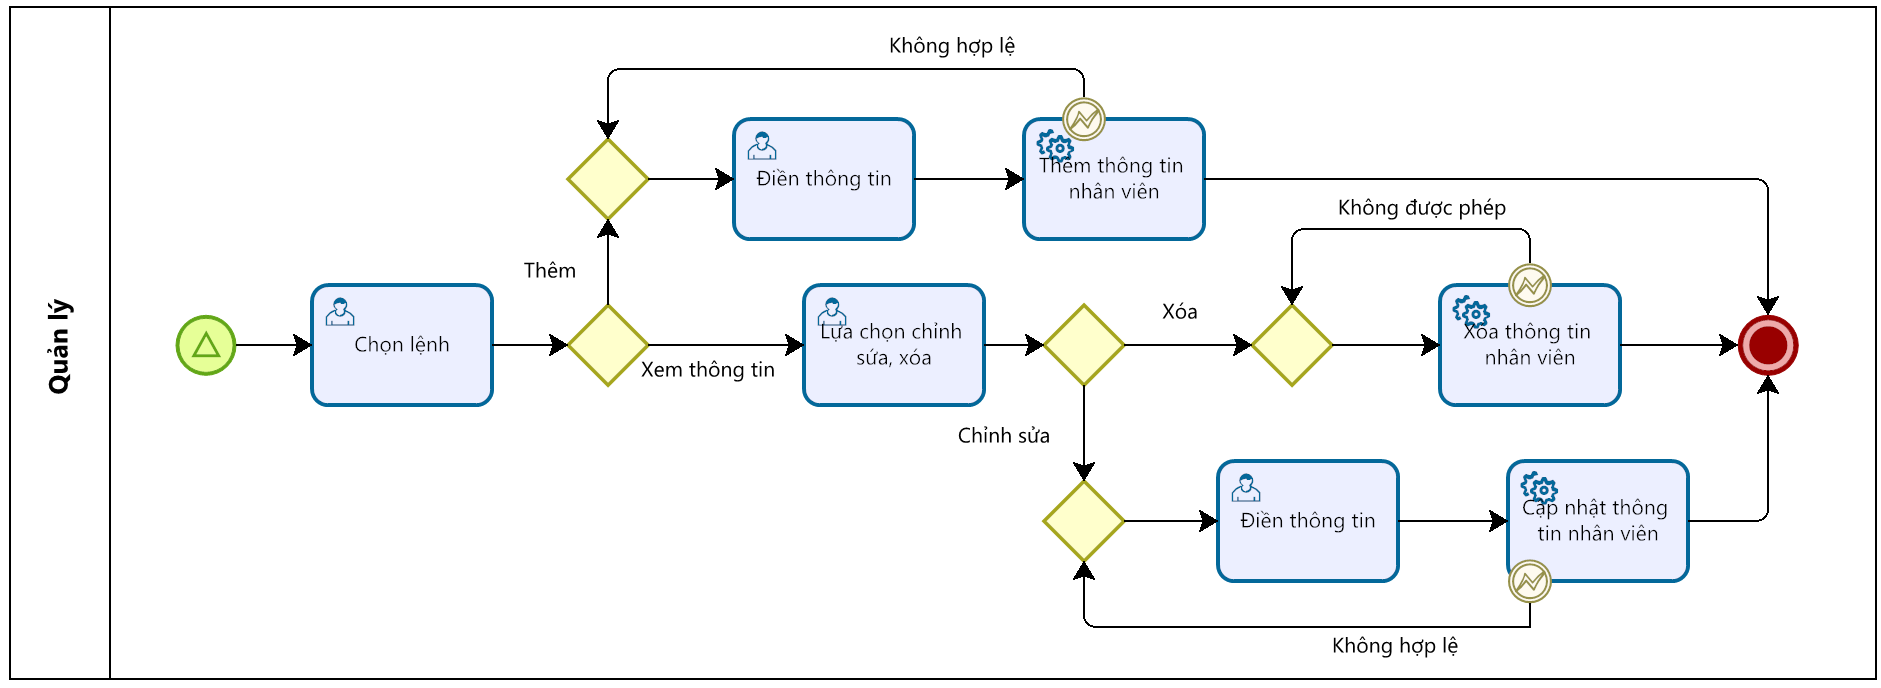
\includegraphics[width=16cm]{img/BPMN/Hien/Employee_Management.png}
	\newline
	\caption{Lược đồ BPMN cho quy trình quản lý nhân viên}
\end{figure}

Khi quản trị viên truy cập, hệ thống sẽ lấy danh sách nhân viên. Quản trị viên thực hiện thêm mới hoặc xem thông tin nhân viên. Nêu thêm mới, quản trị viên sẽ nhập thông tin nhân viên mới và cập nhật hệ thống, nếu có thông tin không hợp lệ, hệ thống sẽ yêu cầu nhập lại thông tin. Nếu xem thông nhân viên, hệ thống sẽ lấy thông tin chi tiết của nhân viên đó. Quản trị viên có thể chỉ xem thông tin nhân viên, chỉnh sửa thông tin hoặc xóa nhân viên. Nếu chọn xóa, hệ thống sẽ kiểm tra và xóa nếu hợp lệ, ngược lại sẽ hiện thông tin chi tiết nhân viên. Nếu chọn chỉnh sửa, hệ thống yêu cầu nhập thông tin sẽ kiểm tra thông tin nếu hợp lệ sẽ cập nhật thông tin, ngược lại sẽ yêu cầu nhập lại thông tin

\newpage

\subsubsection*{Tạo yêu cầu thêm, xóa nhân viên}
\begin{figure}[!htp]
	\centering
	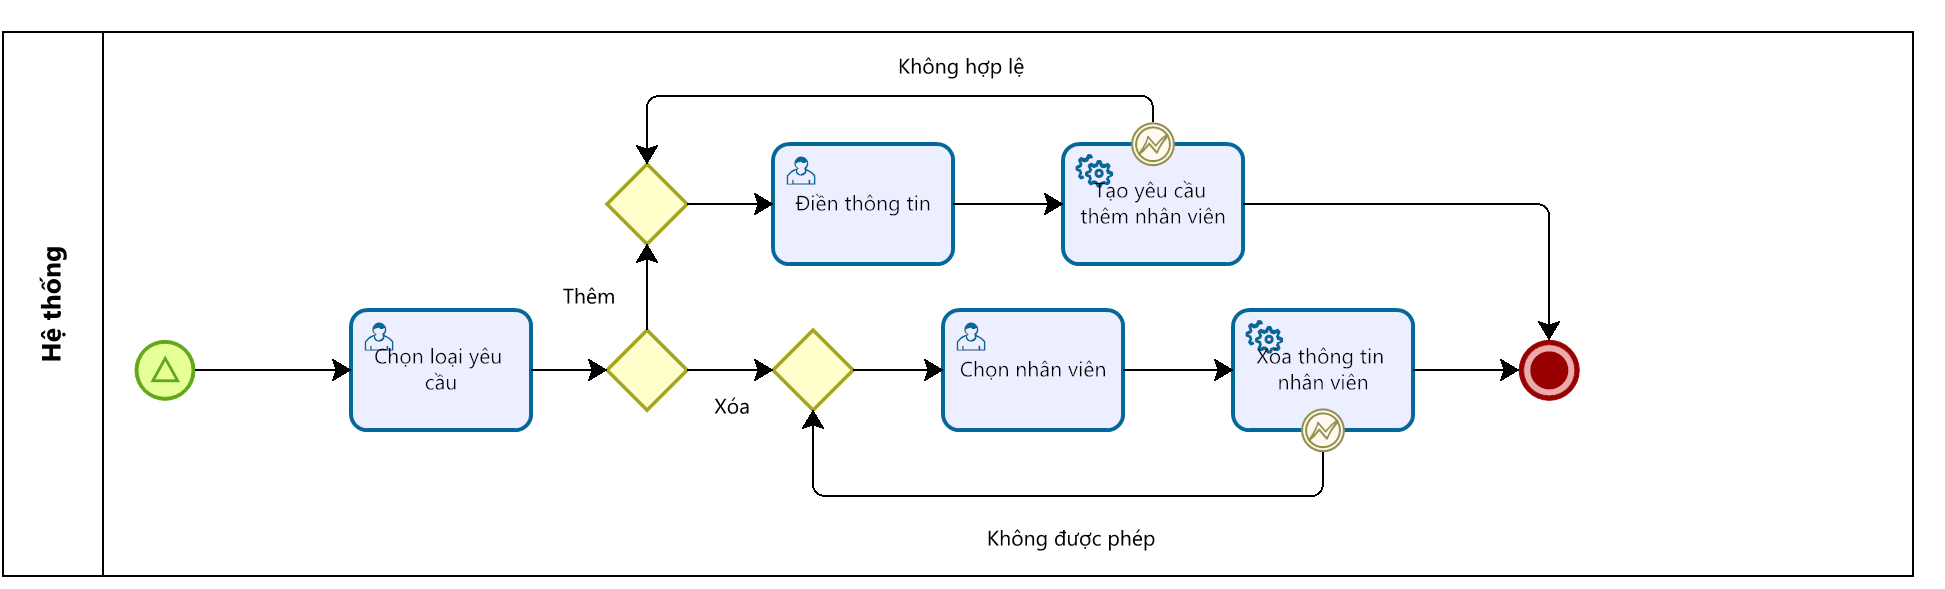
\includegraphics[width=14cm]{img/BPMN/Hien/Employee_request.png}
	\newline
	\caption{Lược đồ BPMN cho quy trình tạo yêu cầu thêm, xóa nhân viên}
\end{figure}

Khi truy cập hệ thống, quản lý có thể chọn loại yêu cầu. Nếu là yêu cầu thêm, hệ thống yêu cầu nhập thông tin nhân viên mới và tạo yêu cầu, nếu thông tin không hợp lệ sẽ phải nhập lại thông tin. Nếu là yêu cầu xóa, hệ thống yêu cầu chọn nhân viên và tạo yêu cầu, nếu không hợp lệ sẽ yêu cầu chọn nhân viên khác

\newpage
% Architecture
% !TeX root = ..\main.tex

\section{Kiến trúc hệ thống}
\subsection{Tổng quan}
\begin{figure}[!htp]
	\centering
	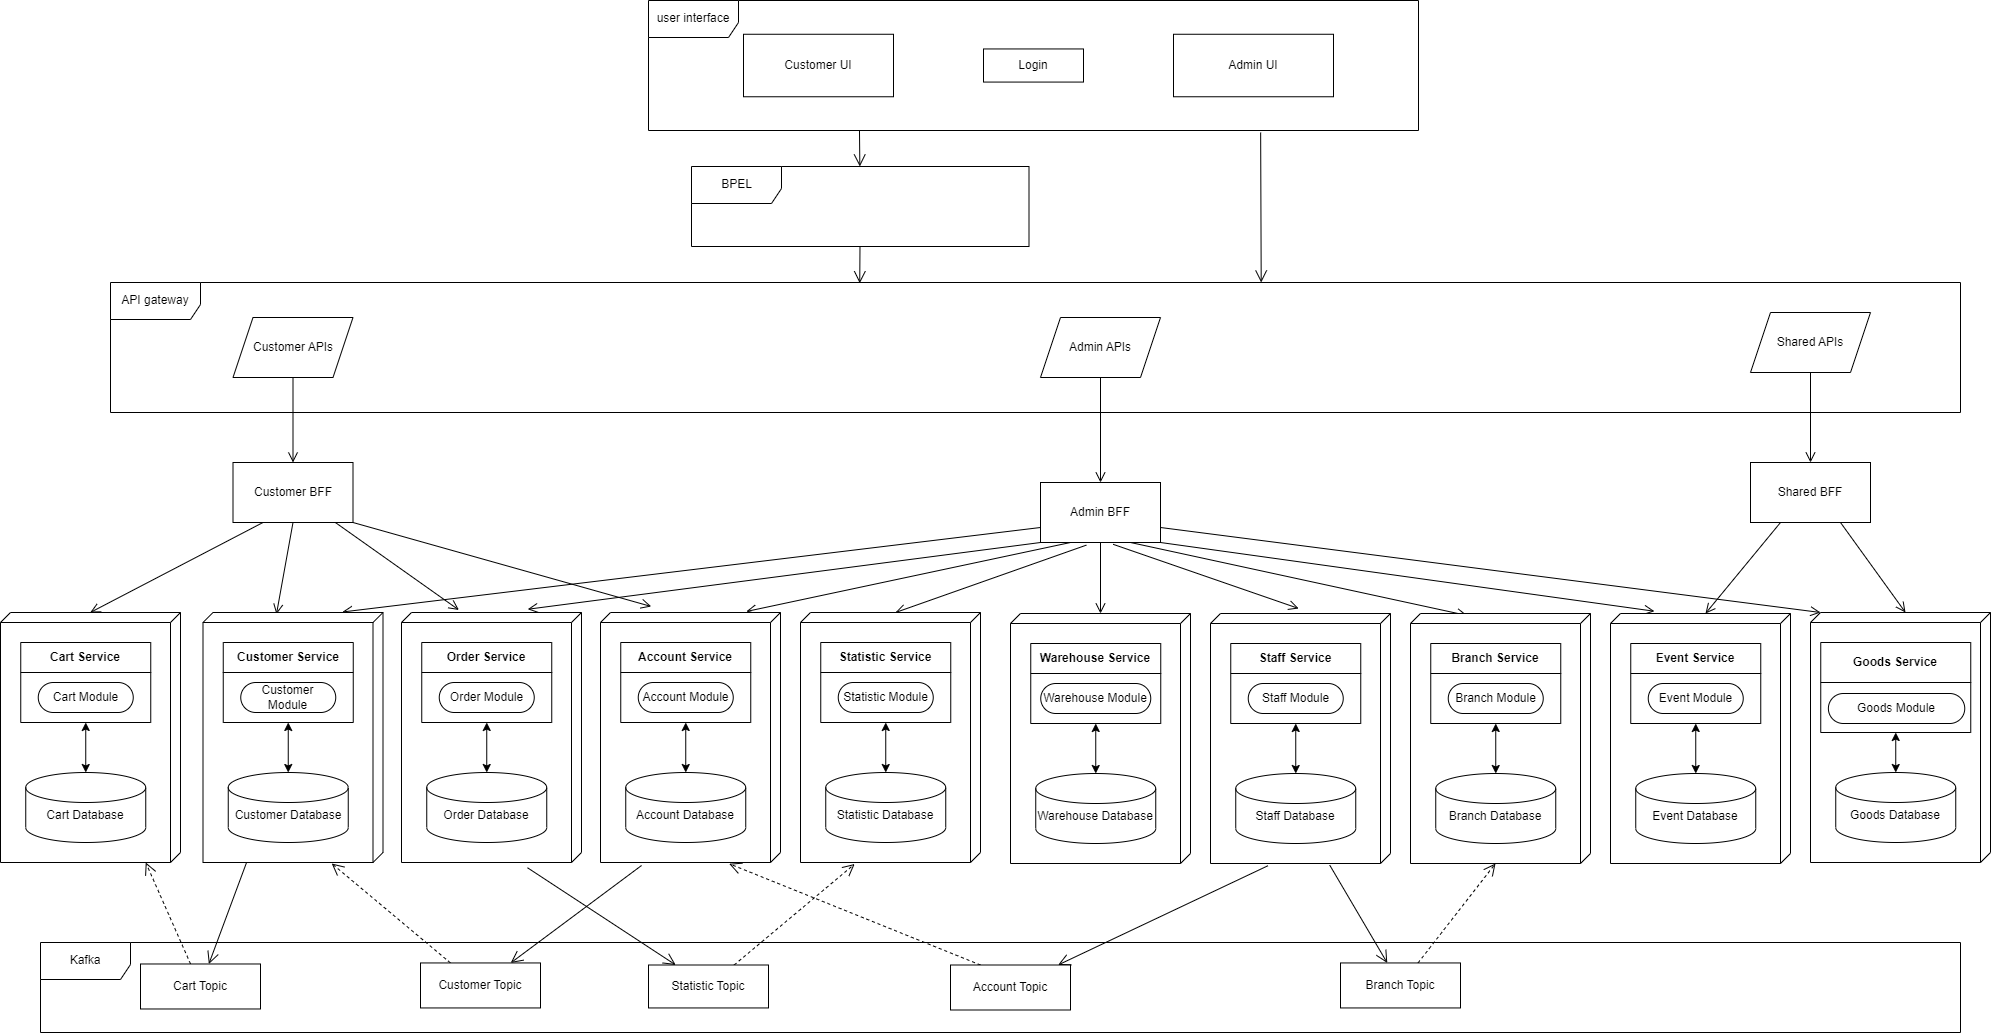
\includegraphics[width=6in]{img/Architecture/general-architect.png}
	\newline
	\caption{Tổng quan kiến trúc hệ thống}
\end{figure}

\subsection{Tầng UI}


\subsubsection{CustomerUI}
Module này bao gồm các class dùng để hiển thị UI đối với phía khách hàng
\begin{figure}[!htp]
	\centering
	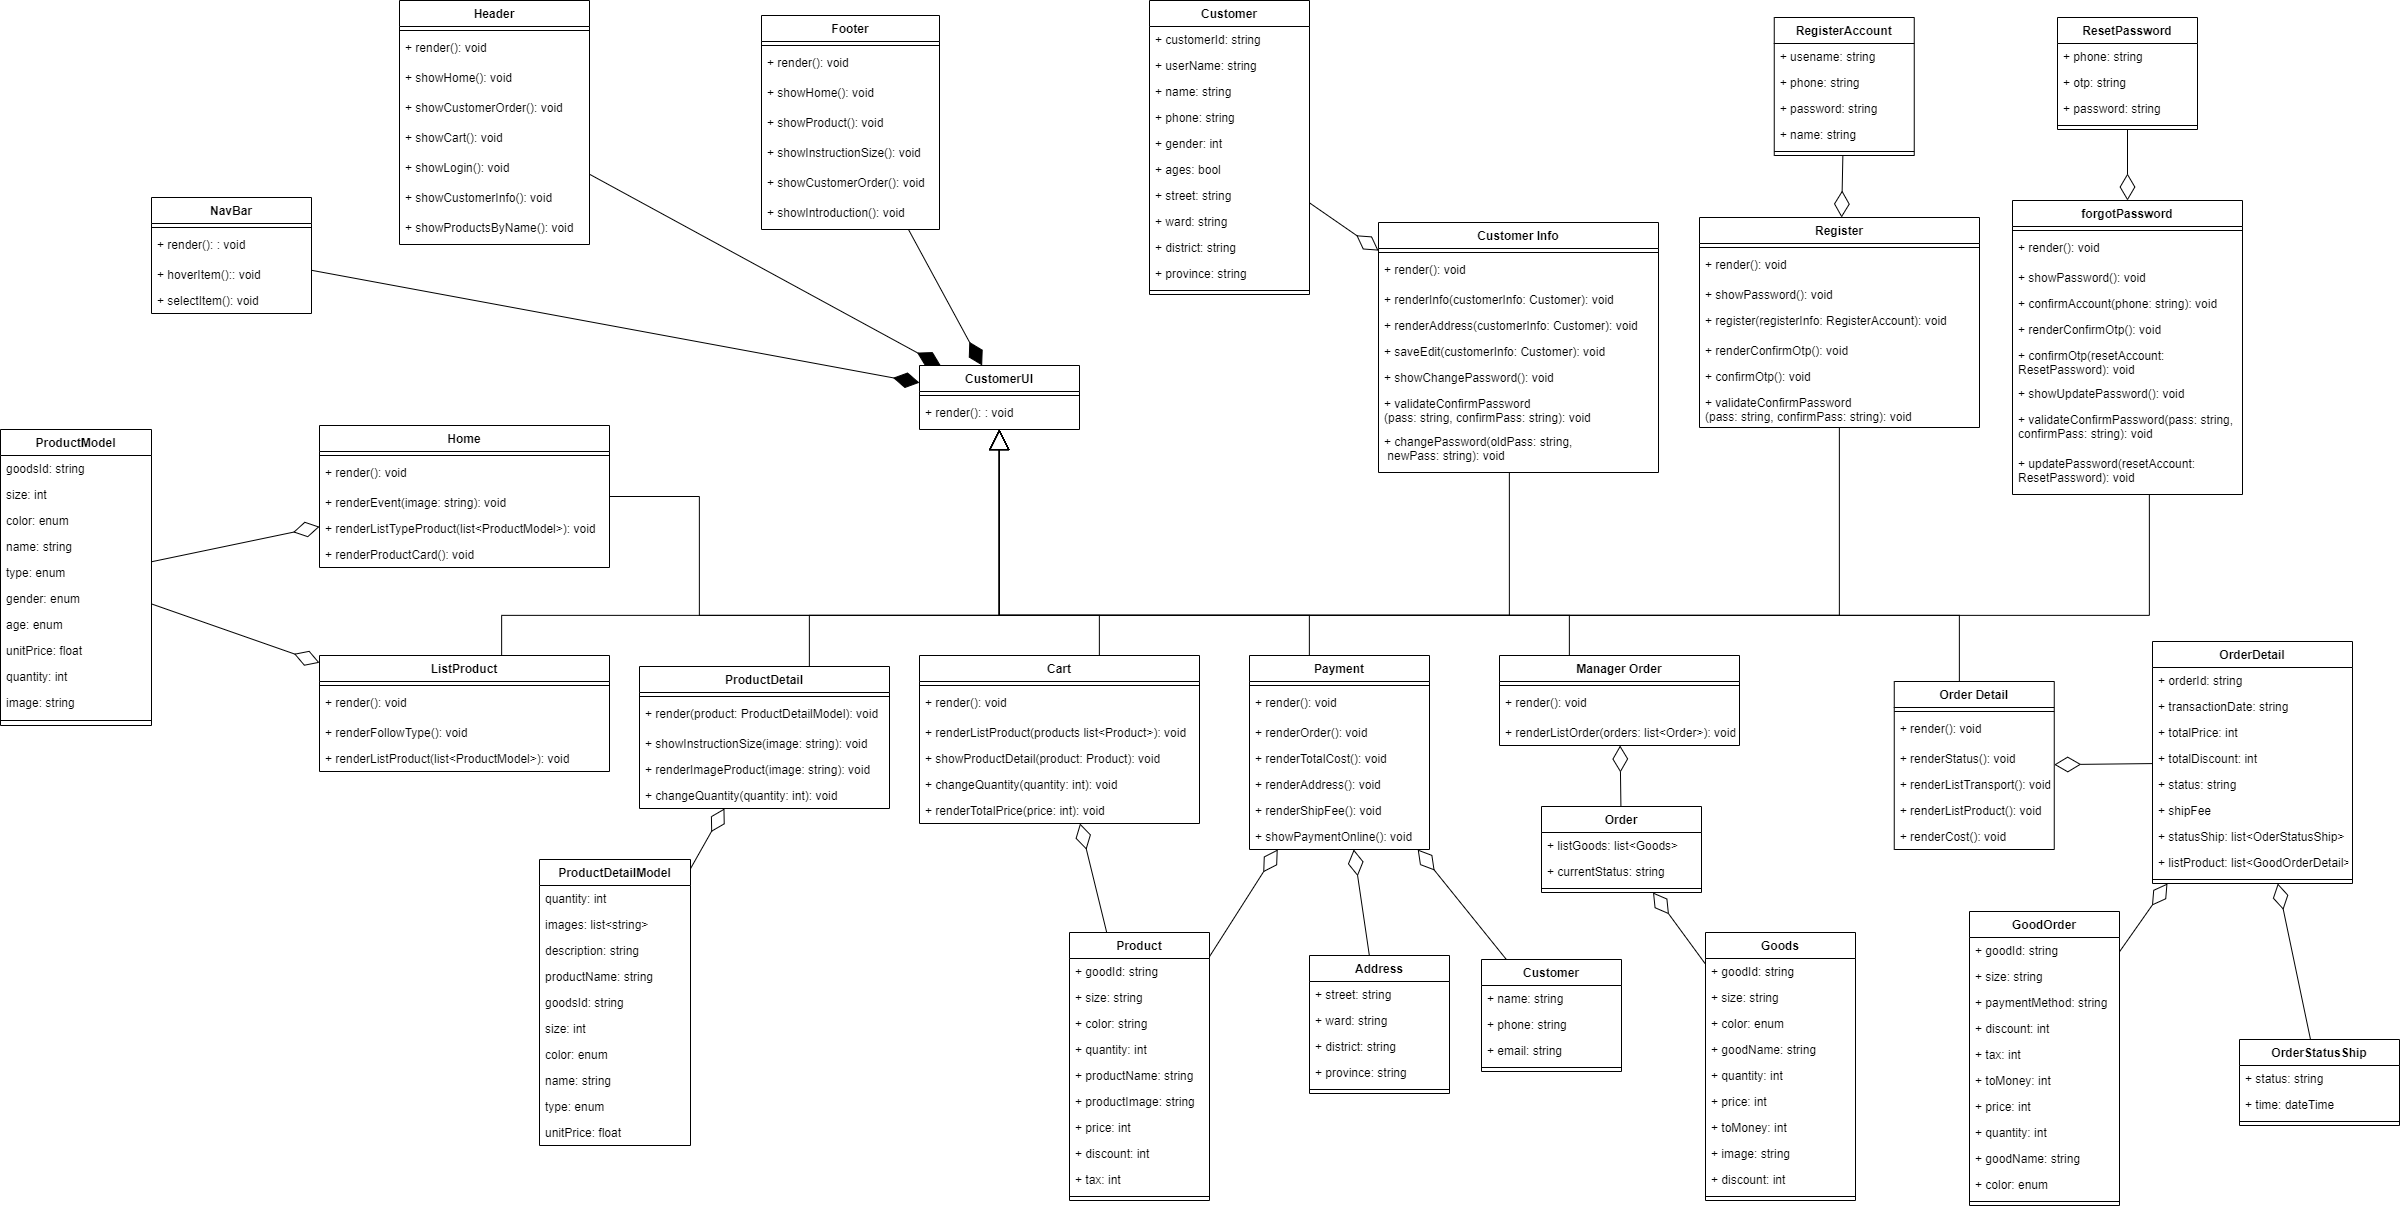
\includegraphics[width=17cm]{img/Architecture/UI/customer UI.png}
	\newline
	\caption{Lược đồ class của Module CustomerUI}
\end{figure}
\textbf{Mô tả:}
\begin{quote}
	\begin{itemize}
		\item CustomerUI: Giao diện chính của khách hàng khi truy cập vào trang web của hệ thống
			\begin{itemize}
				\item render(): Hiển thị lên màn hình của khách hàng
			\end{itemize}
		\item NavBar: Thành phần luôn có của giao diện của khách hàng hiển thị các lựa chọn truy cập nhanh cho khách hàng
			\begin{itemize}
				\item render(): Hiển thị lên màn hình của khách hàng
				\item hoverItem(): Hiển thị lên màn hình giao diện các lựa chọn khi người dùng rê chuột đến các thể loại ở thanh navbar
				\item selectItem(): Hiển thị lên màn hình giao diện tương ứng với lựa chọn của khách hàng trên thanh navbar.
			\end{itemize}
		\item Header: Thành phần luôn có của giao diện của khách hàng hiển thị các thông tin về tài khoản của khách hàng cũng như logo và chức năng tìm kiếm cho khách hàng.
			\begin{itemize}
				\item render(): Hiển thị lên màn hình của khách hàng.
				\item showHome(): Hiển thị về trang chủ mặc định của hệ thống.
				\item showCustomerOrder(): Hiển thị lên màn hình danh sách đơn hàng của khách hàng khi đã đăng nhập.
				\item showCart(): Hiển thị lên màn hình thông tin giỏ hàng của khách hàng khi đã đăng nhập.
				\item showLogin(): Hiển thị lên màn hình trang đăng nhập cho khách hàng khi chưa đăng nhập.
				\item showCustomerInfo(): Hiển thị lên màn hình thông tin chi tiết tài khoản của khách hàng khi đã đăng nhập.
				\item showProductByName(): Hiển thị lên màn hình danh sách các sản phẩm khi người dùng chọn tìm kiếm.
			\end{itemize}
		\item Footer: Thành phần luôn có của giao diện của khách hàng hiển thị các thông tin về hệ thống.
			\begin{itemize}
				\item render(): Hiển thị lên màn hình của khách hàng.
				\item showHome(): Hiển thị về trang chủ mặc định của hệ thống.
				\item showProduct(): Hiển thị lên màn hình danh sách tất cả sản phẩm của hệ thống.
				\item showInstructionSize(): Hiển thị lên màn hình thông tin hướng dẫn chọn size.
				\item showCustomerOrder(): Hiển thị lên màn hình trang danh sách các đơn hàng của khách hàng khi đã đăng nhập.
				\item showIntroduction(): Hiển thị lên màn hình trang giới thiệu về hệ thống cửa hàng.
			\end{itemize}
		\item Home: Màn hình mặc định của người dùng sau khi truy cập vào trang web của hệ thống.
			\begin{itemize}
				\item render(): Hiển thị lên màn hình của khách hàng.
				\item renderEvent(): Hiển thị thông tin các sự kiện đang diễn ra.
				\item renderListTypeProduct(): Hiển thị danh sách các sản phẩm nổi bật theo từng thể loại.
			\end{itemize}
		\item ListProduct: Màn hình hiển thị danh sách tất cả sản phẩm của hệ thống cho khách hàng.
			\begin{itemize}
				\item render(): Hiển thị lên màn hình của khách hàng.
				\item renderFollowType(): Hiển thị danh sách sản phẩm theo đặc điểm và thể loại.
				\item renderListProduct(): Hiển thị danh sách các sản phẩm.
			\end{itemize}
		\item ProductDetail: Màn hình hiển thị danh sách tất cả sản phẩm của hệ thống cho khách hàng.
			\begin{itemize}
				\item render(): Hiển thị lên màn hình của khách hàng.
				\item showInstructionSize(): Hiển thị lên màn hình thông tin hướng dẫn chọn size.
				\item renderImageProduct(): Hiển thị hình ảnh sản phẩm mà khách hàng chọn.
				\item changeQuantity(): Thay đổi số lượng sản phẩm để thêm vào giỏ hàng.
			\end{itemize}
		\item Cart: Màn hình hiển thị thông tin giỏ hàng của khách hàng.
			\begin{itemize}
				\item render(): Hiển thị lên màn hình của khách hàng.
				\item renderListProduct(): Hiển thị danh sách sản phẩm có trong giỏ hàng.
				\item showProductDetail(): Chuyển đến trang thông tin chi tiết của sản phẩm.
				\item changeQuantity(): Thay đổi số lượng sản phẩm trong giỏ hàng.
				\item renderTotalPrice(): Hiển thị tổng giá tiền của các sản phẩm được chọn trong giỏ hàng.
			\end{itemize}
		\item Payment: Màn hình hiển thị trang thanh toán cho khách hàng.
			\begin{itemize}
				\item render(): Hiển thị lên màn hình của khách hàng.
				\item renderOrder(): Hiển thị đơn hàng.
				\item renderTotalCost(): Hiển thị toán bộ chi phí đơn hàng.
				\item renderAddress(): Hiển thị địa chỉ đơn hàng.
				\item renderShipFee(): Hiển thị giá tiền vận chuyển đơn hàng.
				\item ShowPaymentOnline(): Hiển thị màn hình thanh toán online.
			\end{itemize}
		\item Manager Order: Màn hình hiển thị danh sách các đơn hàng của khách hàng.
			\begin{itemize}
				\item render(): Hiển thị lên màn hình của khách hàng.
				\item renderListOrder(): Hiển thị danh sách đơn hàng.
				\item showOrderDetail(): Hiển thị thông tin chi tiết của đơn hàng.
			\end{itemize}
		\item Order Detail: Màn hình hiển thị thông tin chi tiết đơn hàng của khách hàng.
			\begin{itemize}
				\item render(): Hiển thị lên màn hình của khách hàng.
				\item renderStatus(): Hiển thị trạng thái của đơn hàng.
				\item renderListTransport(): Hiển thị danh sách thông tin quá trình vận chuyển.
				\item renderListProduct(): Hiển thị danh sách sản phẩm có trong đơn hàng.
				\item renderCost(): Hiển thị danh sách các khoản chi phí của đơn hàng.
			\end{itemize}
		\item Forgot Password: Màn hình hiển thị trang tạo lại mật khẩu cho tài khoản của khách hàng.
			\begin{itemize}
				\item render(): Hiển thị lên màn hình của khách hàng.
				\item showPassword(): Hiển thị mật khẩu khỏi trạng thái bị ẩn.
				\item confirmAccount(): Xác nhận tài khoản muốn đổi mật khẩu.
				\item renderConfirmOtp(): Hiển thị màn hình xác nhận mã OTP.
				\item confirmOtp(): Gửi xác nhận mã OTP.
				\item showUpdatePassword(): Hiển thị trang cập nhật mật khẩu mới cho tài khoản.
				\item validateConfirmPassword(): Kiểm tra thông tin nhập lại mật khẩu của khách hàng.
				\item updatePassword(): Gửi thông tin cập nhật mật khẩu mới cho tài khoản.
			\end{itemize}
		\item Register: Màn hình hiển thị trang đăng ký tài khoản cho khách hàng.
			\begin{itemize}
				\item render(): Hiển thị lên màn hình của khách hàng.
				\item showPassword(): Hiển thị mật khẩu khỏi trạng thái bị ẩn.
				\item register(): gửi thông tin xác nhận.
				\item renderConfirmOtp(): Hiển thị màn hình xác nhận mã OTP.
				\item confirmOtp(): Gửi xác nhận mã OTP.
				\item validateConfirmPassword(): Kiểm tra thông tin nhập lại mật khẩu của khách hàng.
			\end{itemize}
		\item Customer Info: Màn hình hiển thị trang thông tin chi tiết tài khoản của khách hàng.
			\begin{itemize}
				\item render(): Hiển thị lên màn hình của khách hàng.
				\item renderInfo(): Hiển thị thông tin chung của khách hàng.
				\item renderAddress(): Hiển thị thông tin địa chỉ các khách hàng.
				\item saveEdit(): gửi đi thông tin tài khoản đã chỉnh sửa.
				\item showChangePassword(): hiển thị màn hình đổi mật khẩu.
				\item changePassword(): gửi thông tin đổi mật khẩu của tài khoản.
				\item validateConfirmPassword(): Kiểm tra thông tin nhập lại mật khẩu của khách hàng.
			\end{itemize}
	\end{itemize}
\end{quote}

\subsubsection{LoginUI}
LoginUI là một class dùng để hiển thị trang đăng nhập cho cả phía khách hàng và quản trị viên
\begin{figure}[!htp]
	\centering
	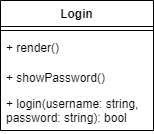
\includegraphics[width=2cm]{img/Architecture/UI/loginUI.png}
	\newline
	\caption{Lược đồ class của LoginUI}
\end{figure}
Phương thức:
\begin{itemize}
	\item showPassword(): Hiện mật khẩu
	\item login(username: string, password: string)(): Đăng nhập vào hệ thống
\end{itemize}

\subsubsection{AdminUI}
Module này bao gồm các class dùng để hiển thị UI đối với phía quản trị viên

\begin{figure}[!htp]
	\centering
	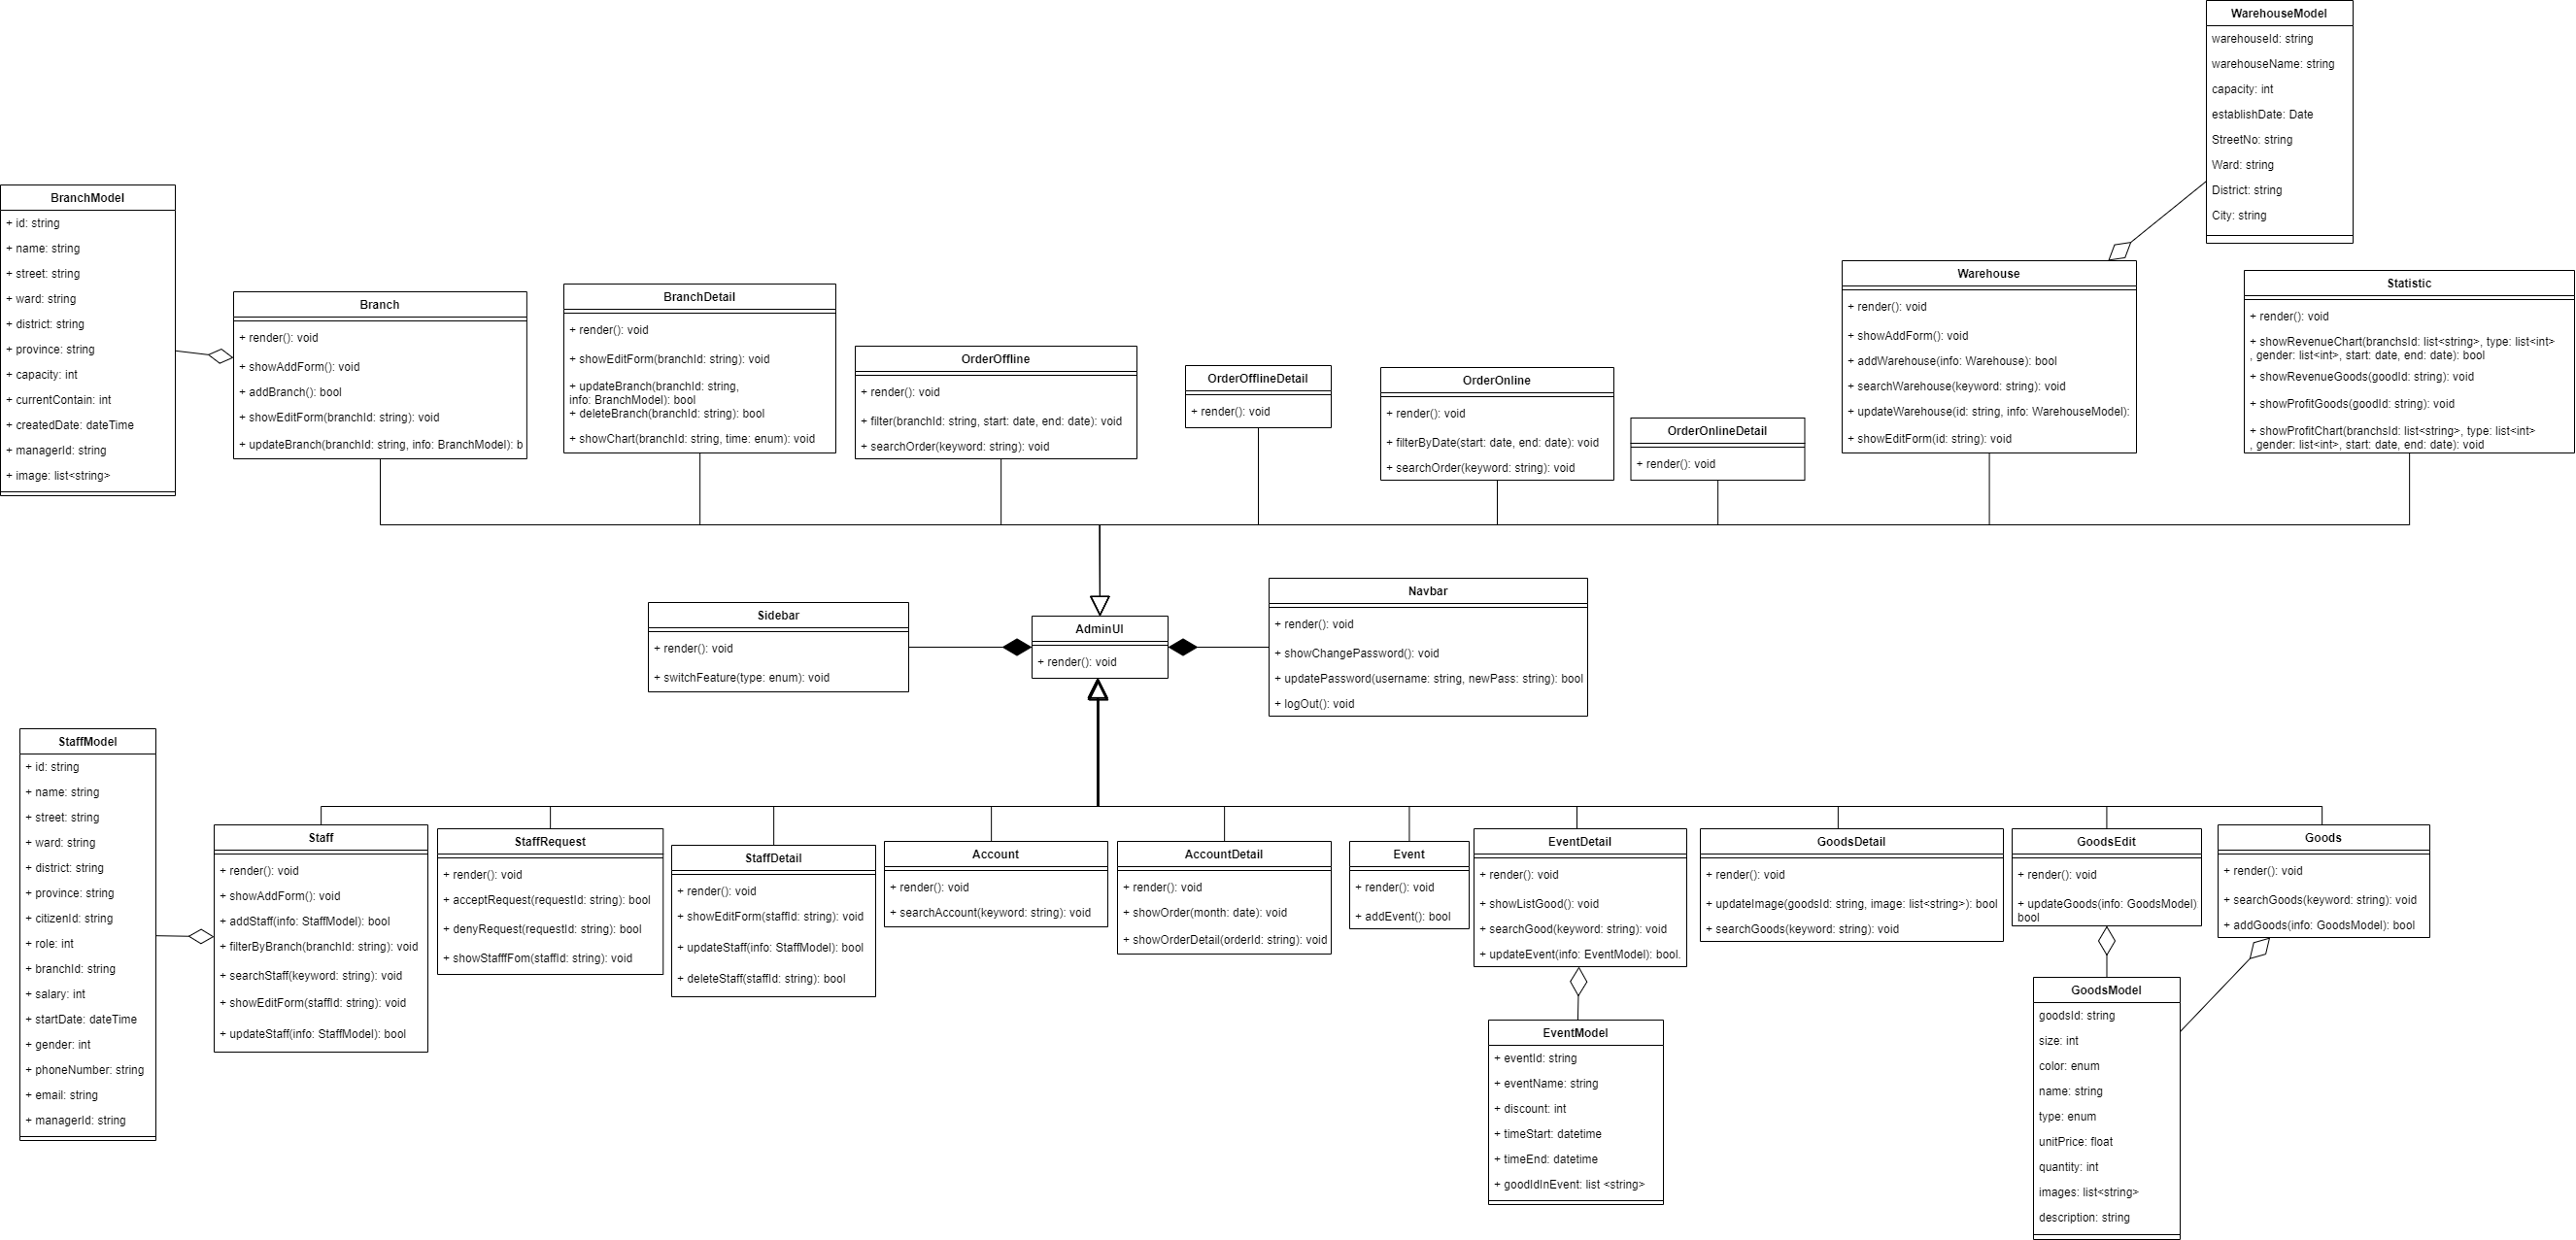
\includegraphics[width=17cm]{img/Architecture/UI/adminUI.png}
	\newline
	\caption{Lược đồ class của Module AdminUI}
\end{figure}

\subsubsubsection*{AdminUI}
Phương thức:
\begin{itemize}
	\item render(): Trình chiếu màn hình admin
\end{itemize}

\subsubsubsection*{Branch}
Phương thức:
\begin{itemize}
	\item showAddForm(): Trình chiếu biểu mẫu thêm mới
	\item addBranch(): Thêm chi nhánh mới
	\item showEditForm(branchId: string): Trình chiếu biểu mẫu chỉnh sửa
	\item updateBranch(branchId: string, info: BranchModel): Cập nhật thông tin chi nhánh
\end{itemize}

\subsubsubsection*{BranchDetail}
Phương thức:
\begin{itemize}
	\item showEditForm(branchId: string): Trình chiếu biểu mẫu chỉnh sửa
	\item updateBranch(branchId: string, info: BranchModel): Cập nhật thông tin chi nhánh
	\item deleteBranch(branchId: string): Xóa chi nhánh
	\item showChart(branchId: string, time: enum): Trình chiếu biểu đồ kinh doanh 
\end{itemize}

\subsubsubsection*{Staff}
Phương thức:
\begin{itemize}
	\item showAddForm(): Trình chiếu biểu mẫu thêm mới
	\item addStaff(info: StaffModel): Thêm một nhân viên
	\item filterByBranch(branchId: string): Tìm nhân viên theo chi nhánh
	\item searchStaff(keyword: string): Tìm kiếm chi nhánh theo từ khóa
	\item showEditForm(staffId: string): Trình chiếu biểu mẫu chỉnh sửa
	\item updateStaff(branchId: string, info: BranchModel): Cập nhật thông tin chi nhánh
\end{itemize}

\subsubsubsection*{StaffRequest}
Phương thức:
\begin{itemize}
	\item acceptRequest(requestId: string): Xác nhận yêu cầu
	\item denyRequest(requestId: string): Hủy bỏ yêu cầu
	\item showStafffFom(staffId: string): Trình chiếu biểu mẫu thông tin nhân viên
\end{itemize}


\subsubsubsection*{StaffDetail}
Phương thức:
\begin{itemize}
	\item showEditForm(staffId: string): Trình chiếu biểu mẫu chỉnh sửa
	\item updateStaff(info: StaffModel): Cập nhật thông tin nhân viên
	\item deleteBranch(staffId: string): Xóa nhân viên
\end{itemize}

\subsubsubsection*{Account}
Phương thức:
\begin{itemize}
	\item searchAccount(keyword: string): Tìm kiếm tài khoản theo từ khóa
\end{itemize}


\subsubsubsection*{AccountDetail}
Phương thức:
\begin{itemize}
	\item showOrder(month: date): Trình chiếu danh sách đơn hàng
	\item showOrderDetail(orderId: string): Trình chiếu biểu mẫu chi tiết đơn hàng  
\end{itemize}

\subsubsubsection*{Event}
Phương thức:
\begin{itemize}
	\item addEvent(): Thêm một sự kiện mới
\end{itemize}

\subsubsubsection*{AccountDetail}
Phương thức:
\begin{itemize}
	\item showListGood(): Trình chiếu danh sách tất cả hàng
	\item searchGood(keyword: string): Tùm kiếm danh sách hàng theo từ khóa
	\item updateEvent(info: EventModel): Cập nhật thông tin sự kiện
\end{itemize}

\subsubsubsection*{Goods}
Phương thức:
\begin{itemize}
	\item searchGoods(keyword: string): Tìm kiếm hàng theo từ khóa
	\item addGoods(info: GoodsModel): Thêm một sản phẩm
\end{itemize}

\subsubsubsection*{GoodsDetail}
Phương thức:
\begin{itemize}
	\item updateImage(goodsId: string, image: list<string>): Cập nhật hình ảnh sản phẩm
	\item searchGoods(keyword: string): Tìm kiếm hàng theo từ khóa
\end{itemize}

\subsubsubsection*{GoodsDetail}
Phương thức:
\begin{itemize}
	\item updateGoods(info: GoodsModel): Cập nhật thông tin sản phẩm
\end{itemize}

\subsubsubsection*{OrderOffline}
Phương thức:
\begin{itemize}
	\item filter(branchId: string, start: date, end: date): Tìm kiếm đơn hàng theo thời gian, chi nhánh
	\item searchOrder(keyword: string): Tìm kiếm đơn hàng theo từ khóa
\end{itemize}

\subsubsubsection*{OrderOnline}
Phương thức:
\begin{itemize}
	\item filter(start: date, end: date): Tìm kiếm đơn hàng theo thời gian
	\item searchOrder(keyword: string): Tìm kiếm đơn hàng theo từ khóa
\end{itemize}





\subsection{Tầng API}
\subsubsection{Customer APIs}
Module này dùng để chứa các API được xuất ra ngoài cho phía khách hàng

\subsubsection{Admin APIs}
Module này dùng để chứa các API được xuất ra ngoài cho phía quản trị viên

\subsubsection{Shared APIs}
Module này dùng để chứa các API được xuất ra ngoài cho bất kì đối tượng người dùng nào




\subsection{Tầng service}

Lược đồ class ở tậng service được xây dựng theo các thành phần sau:
\begin{itemize}
	\item Repository: Class dùng để truy cập trực tiếp đến dữ liệu trong Database
	\item Model: Class dùng để chứa thông tin nhận lên từ Database
	\item Controllers: Class dùng để xử lý các logic nghiệp vụ
	\item Response: Class chứa thông tin trả về khi có yêu cầu từ bên ngoài
	\item Các Interface: Giúp đảm bảo nguyên lý \textbf{Dependency inversion principle} của \textbf{SOLID}
	      \begin {itemize}
	\item IRepository: Cung cấp các api cho các class Controller
	\item IController: Cung cấp các api để bên ngoài service truy cập đến
\end{itemize}
\end{itemize}



\subsubsection{Customer Order Service}
\begin{figure}[!htp]
	\centering
	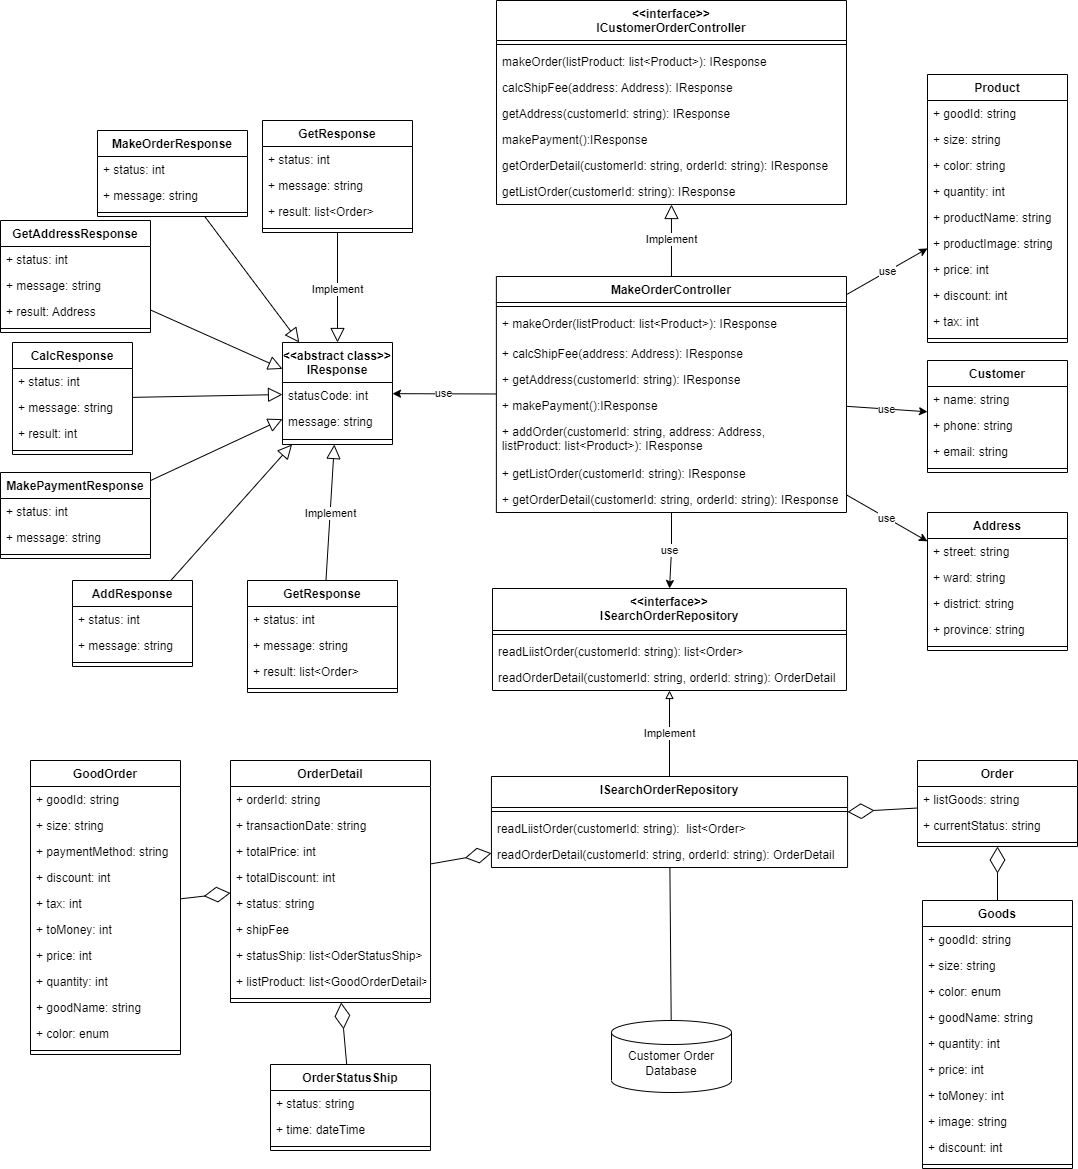
\includegraphics[width=13cm]{img/Architecture/service/CustomerOrderService.png}
	\newline
	\caption{Lược đồ class của Customer Order Service}
\end{figure}

	\subsubsubsection*{CustomerOrderRepository}
	Thuộc tính:
	\begin{itemize}
		\item order: Chứa đối tượng Order
		\item orderDetail: Chứa đối tượng OrderDetail
	\end{itemize}
	Phương thức:
	\begin{itemize}
		\item readListOrder(customerId: string): Lấy danh sách đơn hàng theo mã khách hàng
		\item readOrderDetail(customerId: string, orderId: string): Lấy thông tin chi tiết của đơn hàng.
	\end{itemize}

	\subsubsubsection*{CustomerOrderController}
	Thuộc tính:
	\begin{itemize}
		\item repo: Chứa đối tượng CustomerOrderRepository
	\end{itemize}
	Phương thức:
	\begin{itemize}
		\item makeOrder(listProduct: list<Product>): Tạo đơn hàng
		\item calcShipFee(address: Address): Tính chi phí giao hàng
		\item getAddress(customerId: string): Lấy thông tin địa chỉ của tài khoản của khách hàng.
		\item makePayment(customerId: string): Tạo giao dịch thanh toán.
		\item addOrder(customerId: string, address: Address, listProduct: list<Product>): Thêm đơn hàng vào cơ sở dữ liệu của hệ thống.
		\item getListOrder(customerId: string): Lấy danh sách đơn hàng theo mã khách hàng
		\item getOrderDetail(customerId: string, orderId: string): Lấy thông tin chi tiết của đơn hàng.
	\end{itemize}

	\subsubsubsection*{MakeOrderResponse - GetAddressResponse - CalcResponse - MakePaymentResponse - AddResponse}
	Thuộc tính:
	\begin{itemize}
		\item statusCode: Mã trạng thái của phản hồi
		\item message: Thông điệp của phản hồi
		\item value: Các dữ liệu trả về đối với các yêu cầu
	\end{itemize}
	

\subsubsection{Cart Service}
\begin{figure}[!htp]
	\centering
	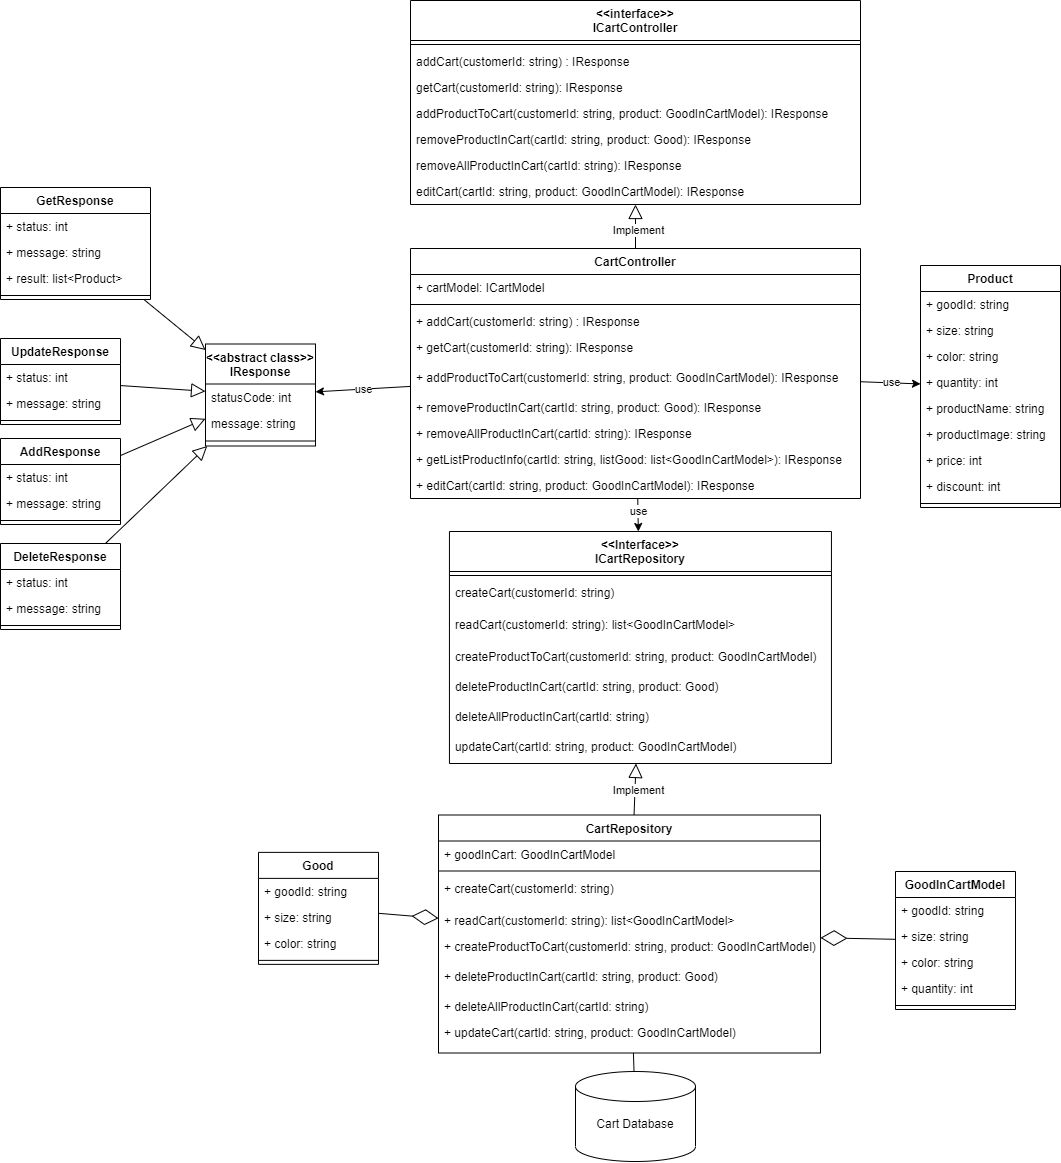
\includegraphics[width=11cm]{img/Architecture/service/CartService.png}
	\newline
	\caption{Lược đồ class của Cart Service}
\end{figure}


\subsubsection{Customer Service}
\begin{figure}[!htp]
	\centering
	\includegraphics[width=11cm]{img/Architecture/service/CustomerService.png}
	\newline
	\caption{Lược đồ class của Customer Service}
\end{figure}



\subsubsection{Order Service}
\begin{figure}[!htp]
	\centering
	\includegraphics[width=11cm]{img/Architecture/service/OrderService.png}
	\newline
	\caption{Lược đồ class của Order Service}
\end{figure}



\subsubsection{Account Service}
\begin{figure}[!htp]
	\centering
	\includegraphics[width=11cm]{img/Architecture/service/AccountService.png}
	\newline
	\caption{Lược đồ class của Account Service}
\end{figure}

\subsubsubsection*{AccountRepository}
Thuộc tính:
\begin{itemize}
	\item accountModel: Chứa đối tượng AccountModel
\end{itemize}
Phương thức:
\begin{itemize}
	\item getAcount(keyword: string): Lấy danh sách tài khoản theo từ khóa
	\item createAccount(info: AccountModel): Tạo một tài khoản mới
	\item updateAccount(info: AccountModel): Cập nhật thông tin một tài khoản
\end{itemize}

\subsubsubsection*{AccountModel}
Thuộc tính:
\begin{itemize}
	\item username: Tên đăng nhập tài khoản
	\item password: Mật khẩu tài khoản
	\item role: Quyền của tài khoản
\end{itemize}

\subsubsubsection*{AccountController}
Thuộc tính:
\begin{itemize}
	\item repo: Chứa đối tượng AccountRepository
\end{itemize}
Phương thức:
\begin{itemize}
	\item getAcount(username: string): Lấy tài khoản theo tên đăng nhập
	\item getListAccount(): Lấy danh sách tất cả tài khoản
	\item searchAccount(keyword: string) : Lấy danh sách tài khoản theo từ khóa
	\item addAccount(info: accountModel): Tạo một tài khoản mới
	\item resetPassword(username: string, newPass: string): Tái thiết lập mật khẩu	
	\item updateRole(username: string, role: int): Cập nhật quyền tài khoản
\end{itemize}


\subsubsubsection*{UpdateResponse - GetResponse}
Thuộc tính:
\begin{itemize}
	\item statusCode: Mã trạng thái của phản hồi
	\item message: Thông điệp của phản hồi
	\item value: Các dữ liệu trả về đối với các yêu cầu HTTP GET
\end{itemize}




\subsubsection{Staff Service}
\begin{figure}[!htp]
	\centering
	\includegraphics[width=11cm]{img/Architecture/service/StaffService.png}
	\newline
	\caption{Lược đồ class của Staff Service}
\end{figure}

\subsubsubsection*{StaffRepository}
Thuộc tính:
\begin{itemize}
	\item staffModel: Chứa đối tượng StaffModel
	\item attendanceModel: Chứa đối tượng AttendanceModel
	\item requestModel: Chứa đối tượng RequestModel
\end{itemize}
Phương thức:
\begin{itemize}
	\item getListStaff(keyword: string): Lấy danh sách nhân viên theo từ khóa
	\item getDetailStaff(id: string): Lấy thông tin chi tiết một nhân viên
	\item createStaff(info: StaffModel): Thêm một nhân viên mới
	\item updateStaff(info: StaffModel): Cập nhật thông tin một nhân viên
	\item deleteStaff(id: string): Xóa một nhân viên
	\item getListAttendance(staffId, month: dateTime): Lấy danh sách điểm danh của nhân viên
	\item createRequest (type: int, info: StaffModel): Tạo một yêu cầu về thêm, xóa nhân viên
	\item updateRequestStatus (status: int, requestId: string): Cập nhật trạng thái cùa yêu cầu
\end{itemize}

\subsubsubsection*{StaffModel}
Thuộc tính:
\begin{itemize}
	\item id: Id của nhân viên
	\item name: Tên của nhân viên
	\item requestModel: Chứa đối tượng RequestModel
	\item street: Tên đường của nhân viên
	\item ward: Phường của nhân viên
	\item distric: Quận của nhân viên
	\item province: Tỉnh của nhân viên
	\item citizenId: Căn cước của nhân viên
	\item role: Vị trí của nhân viên
	\item branchId: Id nơi làm việc của nhân viên
	\item salary: Mức lương của nhân viên
	\item startDate: Ngày bắt đầu làm việc của nhân viên
	\item endDate: Ngày kết thúc làm việc của nhân viên
	\item gender: Giới tính của nhân viên
	\item phoneNumber: Số điện thoại của nhân viên
	\item email: Email của nhân viên
\end{itemize}


\subsubsubsection*{AttendaceModel}
Thuộc tính:
\begin{itemize}
	\item staffId: Id của nhân viên
	\item date: Ngày làm việc
	\item start: Thời gian bắt đầu
	\item end: Thờ gian kết thúc
\end{itemize}

\subsubsubsection*{RequestModel}
Thuộc tính:
\begin{itemize}
	\item id: Id của yêu cầu
	\item staffId: Id của nhân viên
	\item createDate: Ngày tạo
	\item type: Loại yêu cầu
	\item status: Trạng thái yêu cầu
\end{itemize}

\subsubsubsection*{StaffController}
Thuộc tính:
\begin{itemize}
	\item repo: Chứa đối tượng StaffRepository
\end{itemize}
Phương thức:
\begin{itemize}
	\item getListStaff(branchId: string): Lấy danh sách nhân viên theo chi nhánh
	\item getDetailStaff(id: string): Lấy thông tin chi tiết một nhân viên
	\item searchStaff(keyword: string): Lấy danh sách nhân viên theo từ khóa
	\item createStaff(info: StaffModel): Thêm một nhân viên mới
	\item updateStaff(info: StaffModel): Cập nhật thông tin một nhân viên
	\item deleteStaff(id: string): Xóa một nhân viên
	\item createAddRequest(info: StaffModel): Tạo một yêu cầu thêm nhân viên
	\item createDeleteRequest(id:string): Tạo một yêu cầu về xóa nhân viên
	\item updateRequestStatus (status: int, requestId: string): Cập nhật trạng thái cùa yêu cầu
	\item getListAttendance(staffId, month: dateTime): Lấy danh sách điểm danh của nhân viên
\end{itemize}

\subsubsubsection*{UpdateResponse - GetResponse}
Thuộc tính:
\begin{itemize}
	\item statusCode: Mã trạng thái của phản hồi
	\item message: Thông điệp của phản hồi
	\item value: Các dữ liệu trả về đối với các yêu cầu HTTP GET
\end{itemize}



\subsubsection{Branch Service}
\begin{figure}[!htp]
	\centering
	\includegraphics[width=10cm]{img/Architecture/service/BranchService.png}
	\newline
	\caption{Lược đồ class của Branch Service}
\end{figure}

\subsubsubsection*{BranchRepository}
Thuộc tính:
\begin{itemize}
	\item branchModel: Chứa đối tượng BranchModel
	\item staffModel: Chứa đối tượng StaffModel
\end{itemize}
Phương thức:
\begin{itemize}
	\item getListBranch(): Lấy danh sách chi nhánh
	\item getDetailBranch(id: string): Lấy thông tin chi tiết một chi nhánh
	\item createBranch(info: BranchModel): Thêm một chi nhánh mới
	\item updateBranch(info: BranchModel): Cập nhật thông tin một chi nhánh
	\item deleteBranch(id: string): Xóa một chi nhánh
	\item getListStaff(BranchId: string): Lấy danh sách nhân viên của chi nhánh
\end{itemize}

\subsubsubsection*{BranchModel}
Thuộc tính:
\begin{itemize}
	\item id: Id của chi nhánh
	\item name: Tên của chi nhánh
	\item street: Tên đường của chi nhánh
	\item ward: Phường của chi nhánh
	\item distric: Quận của chi nhánh
	\item province: Tỉnh của chi nhánh
	\item createdDate: Ngày tạo chi nhánh
	\item managerId: Id của người quản lý
	\item image: Các hình ảnh của chi nhánh
\end{itemize}

\subsubsubsection*{StaffModel}
Thuộc tính:
\begin{itemize}
	\item id: Id của nhân viên
	\item branchId: Id của chi nhánh làm việc
	\item startDate: Thời gian bắt đầu làm việc tại chi nhánh
	\item endDate: Thời gian kết thúc làm việc tại chi nhánh
\end{itemize}

\subsubsubsection*{BranchController}
Thuộc tính:
\begin{itemize}
	\item repo: Chứa đối tượng repository
\end{itemize}
Phương thức:
\begin{itemize}
	\item getListBranch(): Lấy danh sách chi nhánh
	\item getDetailBranch(id: string): Lấy thông tin chi tiết một chi nhánh
	\item addBranch(info: BranchModel): Thêm một chi nhánh mới
	\item updateBranch(info: BranchModel): Cập nhật thông tin một chi nhánh
	\item deleteBranch(id: int): Xóa một chi nhánh
	\item getListStaff(BranchId: string): Lấy danh sách nhân viên của chi nhánh
	\item updateManger(managerId: sring, branchId:string): Cập nhật quản lý chi nhánh
	\item getStatistic(time: enum): Lấy thông tin thống kê lợi nhuận, doanh thu.
\end{itemize}

\subsubsubsection*{UpdateResponse - GetStaffResponse - GetBranchResponse }
Thuộc tính:
\begin{itemize}
	\item statusCode: Mã trạng thái của phản hồi
	\item message: Thông điệp của phản hồi
	\item value: Các dữ liệu trả về đối với các yêu cầu HTTP GET
\end{itemize}



\subsubsection{Event Service}
\begin{figure}[!htp]
	\centering
	\includegraphics[width=11cm]{img/Architecture/service/EventService.png}
	\newline
	\caption{Lược đồ class của Event Service}
\end{figure}


\subsubsection{Warehouse Service}
\begin{figure}[!htp]
	\centering
	\includegraphics[width=11cm]{img/Architecture/service/WarehouseService.png}
	\newline
	\caption{Lược đồ class của Warehouse Service}
\end{figure}


\subsubsection{Statistic Service}
\begin{figure}[!htp]
	\centering
	\includegraphics[width=11cm]{img/Architecture/service/StatisticService.png}
	\newline
	\caption{Lược đồ class của Statistic Service}
\end{figure}

\subsubsubsection*{StatisticRepository}
Thuộc tính:
\begin{itemize}
	\item statisticalModel: Chứa đối tượng StatisticalModel
	\item filterModel: Chứa đối tượng FilterModel
\end{itemize}
Phương thức:
\begin{itemize}
	\item getAllProductStatistical(): Lấy thông tin thống kê tất cả sản phẩm
	\item getProductStatistical(id: string, start:date,
	end:date): Lấy thông tin thống kê của một sản phẩm
	\item addGoods(goods: GoodModel): Cập nhật thông tin hàng vào Database
	\item getStatisticalByType(filter: FilterModel, start:date,
	end:date): Lấy thông tin thống kê các sản phẩm theo bộ lọc
\end{itemize}

\subsubsubsection*{GoodModel}
Thuộc tính:
\begin{itemize}
	\item goodId: Id của mặt hàng
	\item size: Kích thước của hàng
	\item color: Màu sắc của mặt hàng
	\item type: Loại của mặt hàng
	\item gender: Giới tính của mặt hàng
	\item count: Số lượng đã bán của mặt hàng
	\item price: Giá của mặt hàng
	\item cost: Chi phí nhập của mặt hàng
	\item orderId: Mã đơn chứa mặt hàng
	\item date: Ngày tạo đơn
	\item branchId: Mã chi nhánh tạo đơn
\end{itemize}

\subsubsubsection*{FilterModel}
Thuộc tính:
\begin{itemize}
	\item branchIds: Id của chi nhánh cần lọc
	\item gender: Giới tính hàng cần lọc
	\item type: Loại của mặt hàng cần lọc
\end{itemize}

\subsubsubsection*{StatisticController}
Thuộc tính:
\begin{itemize}
	\item repo: Chứa đối tượng StatisticRepository
\end{itemize}
Phương thức:
\begin{itemize}
	\item getProfitByType(filter: FilterModel, start:date,
	end:date): Lấy thông tin lợi nhuận các mặt hàng theo bộ lọc
	\item getProfitProduct(id: string, start:date,
	end:date): Lấy thông tin lợi nhuận của một sản phẩm
	\item getRevenueProduct(id: string, start:date,
	end:date): Lấy thông tin doanh thu các mặt hàng theo bộ lọc
	\item getRevenueByType(filter: FilterModel, start:date,
	end:date): Lấy thông tin doanh thu của một sản phẩm
	\item addGoods(info: BranchModel): Thêm một mặt hàng vào thống kê
\end{itemize}

\subsubsubsection*{UpdateResponse - GetResponse}
Thuộc tính:
\begin{itemize}
	\item statusCode: Mã trạng thái của phản hồi
	\item message: Thông điệp của phản hồi
	\item value: Các dữ liệu trả về đối với các yêu cầu HTTP GET
\end{itemize}



\subsubsection{Goods Service}
\begin{figure}[!htp]
	\centering
	\includegraphics[width=17cm]{img/Architecture/service/GoodsService.png}
	\newline
	\caption{Lược đồ class của Goods Service}
\end{figure}



\newpage
% Database
% !TeX root = ..\main.tex
\section{Thiết kế cơ sở dữ liệu}
\par Nhóm lựa chọn kiến trúc Microservice cho hệ thống, với việc chia ra các service nhỏ và mỗi service có một database riêng phục vụ cho nghiệp vụ của riêng service đó, nên ở đây các database được thiết kế riêng lẻ cho từng service.

\subsection{ERD/EERD}
\subsubsection{Service Khách hàng}
\begin{figure}[!htp]
	\begin{center}
		\includegraphics[width=0.7\textwidth]{img/database/erd/eerd-customer.png}
		\newline
		\caption{ERD cho database của service Khách hàng}
	\end{center}
\end{figure}

\par Database của service Khách hàng bao gồm hai thực thể là Khách hàng và Tài khoản của khách hàng. Thực thể khách hàng chứa các thông tin cá nhân của khách hàng, bao gồm các thuộc tính:
\begin{itemize}
	\item Mã khách hàng: thuộc tính khóa, là mã của khách hàng.
	\item Tên: Là tên của khách hàng.
	\item Giới tính: Là giới tính của khách hàng.
	\item Email: Là email của khách hàng.
	\item Số điện thoại: Là số điện thoại của khách hàng.
	\item Số nhà, đường: Là địa chỉ sô nhà, đường của khách hàng ở.
	\item Phường / xã: Là địa chỉ phường / xã của khách hàng ở.
	\item Quận / huyện: Là địa chỉ quận / huyện của khách hàng ở.
	\item Tỉnh / thành phố: Là địa chỉ tỉnh / thành phố của khách hàng ở.
\end{itemize}

\par Thực thể Tài khoản của khách hàng bao gồm các thuộc tính:
\begin{itemize}
	\item Tên đăng nhập: tên đăng nhập của tài khoản của khách hàng.
\end{itemize}

\par Khách hàng và Tài khoản có mối quan hệ thuộc, đây là mối quan hệ bắt buộc, 1-1: một khách hàng chỉ thuộc 1 tài khoản và 1 tài khoản chỉ dùng cho 1 khách hàng.

\subsubsection{Service Giỏ hàng}
\begin{figure}[!htp]
	\begin{center}
		\includegraphics[width=0.7\textwidth]{img/database/erd/eerd-cart.png}
		\newline
		\caption{ERD cho database của service Giỏ hàng}
	\end{center}
\end{figure}

\par Database của service Giỏ hàng bao gồm hai thực thể là Giỏ hàng và Hàng trong giỏ hàng. Thực thể Giỏ hàng chứa thông tin về giỏ hàng, bao gồm các thuộc tính:
\begin{itemize}
	\item Mã giỏ hàng: thuộc tính khóa, là mã của giỏ hàng.
	\item Mã khách hàng: là mã khách hàng của khách hàng chủ của giỏ hàng đó.
	\item Số lượng món: là thuộc tính dẫn xuất, số lượng loại sản phẩm có trong giỏ hàng.
\end{itemize}

\par Thực thể Hàng trong giỏ hàng chứa thông tin của mặt hàng trong trong giỏ hàng đó. Thực thể này bao gồm các thuộc tính:
\begin{itemize}
	\item Mã hàng: thuộc tính khóa, là mã của loại hàng đó.
	\item Kích thước: thuộc tính khóa, là kích thước của loại hàng đó.
	\item Màu: thuộc tính khóa, là màu sắc của loại hàng đó.
\end{itemize}

\par Giỏ hàng và Hàng có mối quan hệ chứa, Mối quan hệ là M-N. Giỏ hàng tham gia vào mối quan hệ với ràng buộc tham gia không bắt buộc: Giỏ hàng có thể chứa hàng hoặc không, có thể chứa hàng với số lượng khác nhau. Hàng tham gia vào mối quan hệ với ràng buộc tham gia không bắt buộc, một hàng có thể có hoặc không thuộc giỏ hàng nào. Mối quan hệ này có các thuộc tính:
\begin{itemize}
	\item Số lượng: số lượng của món hàng có trong giỏ hàng.
\end{itemize}

\subsubsection{Service Đơn hàng của khách hàng}
\begin{figure}[!htp]
	\begin{center}
		\includegraphics[width=1\textwidth]{img/database/erd/eerd-customer-order.png}
		\newline
		\caption{ERD cho database của service Đơn hàng của khách hàng}
	\end{center}
\end{figure}

\par Database của service Đơn hàng của khách hàng bao gồm hai thực thể là Đơn hàng và Hàng trong đơn hàng. Thực thể Đơn hàng chứa thông tin về đơn hàng, bao gồm các thuộc tính:
\begin{itemize}
	\item Mã đơn hàng: thuộc tính khóa, là mã của đơn hàng.
	\item Mã khách hàng: là mã khách hàng của khách hàng chủ của đơn hàng đó.
	\item Ngày giao dịch: là ngày thực hiện giao dịch của đơn hàng.
	\item Phí ship: là phí vận chuyển của đơn hàng.
	\item Mong đợi: là thời gian ước tính để giao đơn hàng.
	\item Tổng giá tiền: là thuộc tính dẫn xuất, là tổng giá tiền của đơn hàng.
	\item Thông tin trạng thái: là thuộc tính đa trị, là trạng thái của đơn hàng, bao gồm 2 thuộc tính con là Trạng thái và Thời gian. Trạng thái là trạng thái của đơn hàng và thời gian là thời điểm xảy ra trạng thái của đơn hàng.
\end{itemize}

\par Thực thể Hàng trong đơn hàng chứa thông tin của mặt hàng trong trong đơn hàng đó. Thực thể này bao gồm các thuộc tính:
\begin{itemize}
	\item Mã hàng: thuộc tính khóa, là mã của loại hàng đó.
	\item Kích thước: thuộc tính khóa, là kích thước của loại hàng đó.
	\item Màu: thuộc tính khóa, là màu sắc của loại hàng đó.
	\item Số lượng: là số lượng của loại hàng trong đơn hàng.
	\item Đơn giá: là giá tiền của loại hàng trong đơn hàng.
	\item Thuế: là thuế được thu trên loại hàng đó trong đơn hàng.
	\item Thành tiền: là thuộc tính dẫn xuất, giá tiền cuối cùng được tính cho loại hàng đó trong đơn hàng.
\end{itemize}

\par Đơn hàng và Hàng có mối quan hệ Bao gồm, đây là quan hệ bắt buộc, Mối quan hệ là 1-N: đơn hàng bắt buộc có hàng, và có thể có nhiều hàng; hàng trong đơn hàng bắt buộc phải thuộc về một đơn hàng, và chỉ thuộc về duy nhất một đơn hàng.

\subsubsection{Service Sự kiện}
\begin{figure}[!htp]
	\begin{center}
		\includegraphics[width=0.6\textwidth]{img/database/erd/eerd-event.png}
		\newline
		\caption{ERD cho database của service Sự kiện}
	\end{center}
\end{figure}

\par Database của service Sự kiện bao gồm hai thực thể là Sự kiện và Hàng. Thực thể Sự kiện chứa thông tin về sự kiện, bao gồm các thuộc tính:
\begin{itemize}
	\item Mã sự kiện: thuộc tính khóa, là mã của sự kiện.
	\item Tên: là của sự kiện.
	\item Giảm giá: là giá trị giảm giá của sự kiện đối với các mặt hàng trong sự kiện.
	\item Thời gian bắt đầu: là thời gian bắt đầu sự kiện.
	\item Thời gian kết thúc: là thời gian kết thúc sự kiện.
\end{itemize}

\par Thực thể Hàng trong sự kiện chứa thông tin của mặt hàng trong trong sự kiện đó. Thực thể này bao gồm các thuộc tính:
\begin{itemize}
	\item Mã hàng: thuộc tính khóa, là mã của loại hàng đó.
\end{itemize}

\par Sự kiện và Hàng có mối quan hệ có, mối quan hệ là M-N: sự kiện có thể có nhiều hàng, ít hàng hoặc không có hàng; hàng trong cũng có thể thuộc không hoặc ít hoặc nhiều sự kiện.

\subsubsection{Service Hàng hóa}
\begin{figure}[!htp]
	\begin{center}
		\includegraphics[width=1\textwidth]{img/database/erd/shop_online-hàng.png}
		\newline
		\caption{ERD cho database của service Hàng hóa}
	\end{center}
\end{figure}

\par Database của service Hàng hóa bao gồm hai thực thể là Hàng hóa và Hàng trong kho. Thực thể hàng hóa chỉ thông tin các mặt hàng được bán, bao gồm các thuộc tính:
\begin{itemize}
	\item Mã hàng: thuộc tính khóa, là mã của mặt hàng.
	\item Kích thước: thuộc tính khóa, là kích thước của mặt hàng.
	\item Màu: thuộc tính khóa, là màu của mặt hàng.
	\item Tên hàng: là tên của mặt hàng.
	\item Lứa tuổi: là lứa tuổi phù hợp của mặt hàng.
	\item Giới tính: là giới tính phù hợp của mặt hàng.
	\item Nhà sản xuất: là nhà sản xuất của mặt hàng.
	\item Hình ảnh: thuộc tính đa trị, bao gồm các hình ảnh của mặt hàng.
	\item Được bán: cho biết mặt hàng có đang được mở bán hay không.
	\item Đơn giá: giá tiền cho một đơn vị của mặt hàng.
	\item Mô tả: thông tin thêm về mặt hàng.
	\item Loại: thể loại của mặt hàng.
	\item Số lượng hiện tại: thuộc tính dẫn xuất, là số lượng còn tồn hiện tại của mặt hàng.
\end{itemize}

\par Thực thể Hàng trong kho chỉ thông tin của mặt hàng trong một kho nào đó. Thực thể này bao gồm các thuộc tính:
\begin{itemize}
	\item Mã kho: thuộc tính khóa, là mã của kho chứa hàng đó.
	\item Số lượng: số lượng hàng đó còn trong kho.
	\item Ngày tạo: ngày mặt hàng lần đầu vào kho.
	\item Ngày thay đổi: ngày hàng trong kho có sự thay đổi.
\end{itemize}

\par Hàng hóa và Hàng trong kho có mối quan hệ Bao gồm, đây là mối quan hệ bắt buộc, 1-N: hàng hóa bắt buộc phải nằm trong kho, và một mặt hàng có thể nằm ở nhiều kho; hàng trong kho bắt buộc thuộc về một mặt hàng, và chỉ thuộc về duy nhất một mặt hàng.

\subsubsection{Service Đơn hàng}
\begin{figure}[!htp]
	\begin{center}
		\includegraphics[width=1\textwidth]{img/database/erd/shop_online-đơnhàng.png}
		\newline
		\caption{ERD cho database của service Đơn hàng}
	\end{center}
\end{figure}

\par Database của service Đơn hàng bao gồm các thực thể Đơn hàng và Hàng hóa, chỉ các hàng hóa trong đơn hàng. Đơn hàng được cụ thể hóa xuống Đơn hàng online và Đơn hàng cửa hàng.
\par Thực thể Đơn hàng gồm các thuộc tính:
\begin{itemize}
	\item Mã đơn hàng: thuộc tính khóa, chỉ mã của đơn hàng.
	\item Ngày giao dịch: ngày thực hiện giao dịch mua hàng và sinh ra đơn hàng.
	\item Tổng giá tiền: thuộc tính dẫn xuất, là tổng giá tiền của đơn hàng.
\end{itemize}

\par Thực thể Đơn hàng online có thêm các thuộc tính:
\begin{itemize}
	\item Mã khách hàng: là mã khách hàng đã mua hàng online.
	\item Phí ship: giá tiền cho việc vận chuyển đơn hàng.
	\item Mong đợi: ngày giao hàng mong đợi.
	\item Thông tin trạng thái: thuộc tính phức hợp, bao gồm các thông tin Trạng thái và Thời gian chỉ các trạng thái và thời gian đạt đến trạng thái đó của đơn hàng.
\end{itemize}

\par Thực thể Đơn hàng cửa hàng có thêm thuộc tính:
\begin{itemize}
	\item Mã cửa hàng: mã cửa hàng bán hàng trong đơn hàng.
\end{itemize}

\par Thực thể Hàng bao gồm các thuộc tính:
\begin{itemize}
	\item Mã hàng: thuộc tính khóa, là mã của mặt hàng trong đơn hàng.
	\item Kích thước: thuộc tính khóa, là kích thước của hàng trong đơn hàng.
	\item Màu: thuộc tính khóa, là màu của hàng trong đơn hàng.
	\item Số lượng: số lượng hàng đã mua trong đơn hàng.
	\item Đơn giá: giá tiền một đơn vị của hàng trong đơn hàng.
	\item Thuế: giá tiền thuế của hàng trong đơn hàng.
	\item Thành tiền: thuộc tính dẫn xuất, là tổng giá tiền (đơn giá * số lượng) + thuế.
\end{itemize}

\par Đơn hàng và Hàng có quan hệ Bao gồm, đây là quan hệ bắt buộc, 1-N: đơn hàng bắt buộc có hàng, và có thể có nhiều hàng; hàng trong đơn hàng bắt buộc phải thuộc về một mặt hàng, và chỉ thuộc về duy nhất một mặt hàng.

\subsubsection{Service Kho}
\begin{figure}[!htp]
	\begin{center}
		\includegraphics[width=1\textwidth]{img/database/erd/shop_online-Kho.png}
		\newline
		\caption{ERD cho database của service Kho}
	\end{center}
\end{figure}

\par Database của service Kho bao gồm thực thể Kho và thực thể Nhân viên kho. Thực thể Kho bao gồm các thuộc tính:
\begin{itemize}
	\item Mã kho: thuộc tính khóa, là mã của kho.
	\item Tên kho: tên của kho.
	\item Ngày thành lập: ngày mà kho đi vào sử dụng.
	\item Địa chỉ: thuộc tính kết hợp, bao gồm các thuộc tính Số nhà, đường, Phường, Thành phố / Quận / Huyện, Tỉnh / Thành phố.
	\item Sức chứa: sức chứa hàng tối đa của kho.
	\item Còn lại: thuộc tính dẫn xuất, chỉ sức chứa còn lại mà kho có thể chứa hàng thêm.
\end{itemize}

\par Thực thể Nhân viên kho bao gồm các thuộc tính:
\begin{itemize}
	\item Mã nhân viên: thuộc tính khóa, là mã của nhân viên làm việc ở kho.
\end{itemize}

\par Kho và nhân viên kho có mối quan hệ Bao gồm là mối quan hệ bắt buộc, M-N: kho bắt buộc có nhân viên, và có thể có nhiều nhân viên làm việc; nhân viên buộc phải làm việc ở ít nhất một kho, và có thể làm việc ở nhiều kho. Mối quan hệ này có các thuộc tính:
\begin{itemize}
	\item Ngày bắt đầu: ngày nhân viên bắt đầu làm việc tại kho đó.
	\item Ngày kết thúc: ngày nhân viên nghỉ làm việc tại kho đó.
\end{itemize}

\par Mỗi kho có một quản lý, nên kho và nhân viên quản lý có mối quan hệ Được quản lý bởi. Mối quan hệ là M-N. Kho tham gia vào mối quan hệ với ràng buộc tham gia bắt buộc: kho phải có quản lý, và theo thời gian có nhiều quản lý theo từng thời gian khác nhau. Quản lý - cũng là nhân viên kho, tham gia vào mối quan hệ với ràng buộc tham gia không bắt buộc, một nhân viên không cần phải làm quản lý, và qua thời gian có thể làm quản lý ở nhiều kho. Mối quan hệ này có các thuộc tính:
\begin{itemize}
	\item Ngày bắt đầu: ngày quản lý bắt đầu làm việc tại kho đó.
	\item Ngày kết thúc: ngày quản lý nghỉ làm việc tại kho đó.
\end{itemize}

\subsubsection{Service chi nhánh}
\begin{figure}[!htp]
	\begin{center}
		\includegraphics[width=1\textwidth]{img/database/erd/branch.png}
		\newline
		\caption{ERD cho database của service chi nhánh}
	\end{center}
\end{figure}

Database của service chi nhánh bao gồm hai thực thể là Nhân viên và chi nhánh. Thực thể chi nhánh chứa thông tin về chi nhánh:
\begin{itemize}
	\item mã: thuộc tính khóa, là mã của chi nhánh.
	\item tên: Tên chi nhánh.
	\item ngày tạo: Ngày tạo chi nhánh.
	\item giờ mở: Giờ mở cửa mổi ngày của chi nhánh.
	\item giờ đóng: Giờ đóng cửa mổi ngày của chi nhánh.
	\item hình ảnh: Hình ảnh minh họa chi nhánh.
	\item đường/thôn: Tên đường của chi nhánh.
	\item phường/xã: Phường xã của chi nhánh.
	\item quận/huyện: Quận, huyện của chi nhánh.
	\item thành phố /tỉnh: Tỉnh, thành phố của chi nhánh
\end{itemize}

Thực thể Nhân viên chỉ chứa một vài thông tin nhân viên:
\begin{itemize}
	\item mã: thuộc tính khóa, là mã của nhân viên.
\end{itemize}

Chi nhánh và nhân viên có mối quan hệ Làm tại và Quản lý: Mỗi chi nhánh đều phải có ít nhất một nhân viên và một quản lý. Mối quan hệ Bao gồm có các thông tin:
\begin{itemize}
	\item ngày bắt đầu: ngày bắt đầu làm việc tại chi nhánh của nhân viên.
	\item ngày kết thúc: ngày kết thúc làm việc tại chi nhánh của nhân viên.
\end{itemize}


\subsubsection{Service tài khoản}
\begin{figure}[!htp]
	\begin{center}
		\includegraphics[width=5cm]{img/database/erd/account.png}
		\newline
		\caption{ERD cho database của service tài khoản}
	\end{center}
\end{figure}

Database của service tài khoản chỉ có thực thể tài khoản chứa thông tin về tài khoản:
\begin{itemize}
	\item tên đăng nhập: Thuộc tính khóa, là tên đăng nhập của tài khoản.
	\item mật khẩu: Mật khẩu của tài khoản.
	\item quyền: Quyền của tài khoản.
\end{itemize}


\subsubsection{Service nhân viên}
\begin{figure}[!htp]
	\begin{center}
		\includegraphics[width=1\textwidth]{img/database/erd/staff.png}
		\newline
		\caption{ERD cho database của service nhân viên}
	\end{center}
\end{figure}

Database của service nhân viên chứa các thực thể Nhân viên, Bản yêu cầu, Tài khoản, Bản điểm danh. Thực thể Nhân viên bao gồm các thông tin của nhân viên:
\begin{itemize}
	\item mã: thuộc tính khóa, là mã của nhân viên.
	\item tên: Tên nhân viên.
	\item cccd: Căn cước công dân chi nhánh
	\item vị trí: Vị trí làm việc trong cửa hàng
	\item lương: Mức lương của nhân viên
	\item ngày vào: Ngày được nhận vào làm.
	\item sdt: Số điện thoại của nhân viên.
	\item email: Email của nhân viên.
	\item đường/thôn: Tên đường của nhân viên.
	\item phường/xã: Phường xã của nhân viên.
	\item quận/huyện: Quận, huyện của nhân viên.
	\item thành phố /tỉnh: Tỉnh, thành phố của nhân viên
\end{itemize}

Thực thể Bản yêu cầu chứa thông tin về yêu cầu thêm, xóa nhân viên:
\begin{itemize}
	\item mã: thuộc tính khóa, là mã của yêu cầu.
	\item ngày yêu cầu: Ngày tạo yêu cầu
	\item loại yêu cầu: Loại của yêu cầu là thêm hay xóa
	\item trạng thái: Trạng thái của yêu cầu đang chờ, được duyệt hoặc hủy bỏ
\end{itemize}

Thực thể Bản điểm danh chứa thông tin về hoạt động điểm danh của nhân viên:
\begin{itemize}
	\item ngày: thuộc tính khóa, là ngày làm việc của nhân viên.
	\item thời gian vào: Thời gian bắt đầu vào làm trong ngày của nhân viên
	\item thời gian ra: Thời gian kết thúc làm trong ngày của nhân viên
	\item thời gian làm: Thời gian làm việc trong ngày của nhân viên
\end{itemize}

Thực thể Tài khoản chỉ chứa thông tin về tên tài khoản của nhân viên

Nhân viên và Bản yêu cầu có mối quan hệ Thuộc về: Mỗi bản yêu cầu đều phải thuộc về một nhân viên

Nhân viên và Tài khoản có mối quan hệ Có: Chỉ có các nhân viên cấp quản lý mới sở hữu tài khoản

Nhân viên và Bản điểm danh cầu có mối quan hệ Điểm danh: Tât cả bản điểm danh đều phải có nhân viên


\subsubsection{Service thống kê}
\begin{figure}[!htp]
	\begin{center}
		\includegraphics[width=1\textwidth]{img/database/erd/Statistic.png}
		\newline
		\caption{ERD cho database của service thống kê}
	\end{center}
\end{figure}

Database của service chi nhánh bao gồm hai thực thể là Đơn hàng và hàng. Thực thể đơn hàng chứa thông tin về các đơn hàng:
\begin{itemize}
	\item Mã đơn hàng: thuộc tính khóa, là mã của đơn hàng.
	\item Ngày giao dịch: Ngày tạo đơn hàng.
	\item mã cửa hàng: Nơi tạo đơn hàng.
\end{itemize}

Thực thể Hàng chỉ chứa một vài thông tin của hàng hóa được bán:
\begin{itemize}
	\item Mã hàng: thuộc tính khóa, là mã của món hàng.
	\item Kích thước: thuộc tính khóa, là kích thước của món hàng.
	\item Màu: thuộc tính khóa, là mã của món hàng.
	\item Loại: Loại của món hàng.
	\item Số lượng: Số lượng của món hàng trong đơn.
	\item Giới tính: Giới tính của món hàng.
	\item chi phí: Giá nhập của món hàng.
	\item đơn giá: Đơn giá bán ra của món hàng.
\end{itemize}

Đơn hàng và hàng có mối quan hệ bao gồm: Mỗi đơn hàng đều phải có ít nhất một món hàng và mỗi món hàng đều phải nằm trong ít nhất một đơn hàng:


\subsection{Ánh xạ}
\par Từ các ERD/EERD trên, chúng ta có các ánh xạ sau tương ứng với mỗi service.

\subsubsection{Service Khách hàng}
\begin{figure}[!htp]
	\begin{center}
		\includegraphics[width=1\textwidth]{img/database/mapping/mapping-customer.png}
		\newline
		\caption{Ánh xạ cho database của service Khách hàng}
	\end{center}
\end{figure}

Bảng dữ liệu Khách hàng trong service Khách hàng bao gồm các thuộc tính và kiểu dữ liệu như sau:
\begin{itemize}
	\item Mã khách hàng: string.
	\item Tên đăng nhập: string.
	\item Tên: string.
	\item Email: string.
	\item Số điện thoại: string.
	\item Giới tính: string.
	\item Đường: string.
	\item Phường\_xã: string.
	\item Quận\_huyện: string.
	\item Tỉnh\_thành: string.
\end{itemize}

\subsubsection{Service Giỏ hàng}
\begin{figure}[!htp]
	\begin{center}
		\includegraphics[width=1\textwidth]{img/database/mapping/mapping-cart.png}
		\newline
		\caption{Ánh xạ cho database của service Giỏ hàng}
	\end{center}
\end{figure}

Bảng dữ liệu Giỏ hàng trong service Giỏ hàng bao gồm các thuộc tính và kiểu dữ liệu như sau:
\begin{itemize}
	\item Mã giỏ hàng: string.
	\item Mã khách hàng: string.
	\item Số lượng: int.
	\item Mã hàng: string.
	\item Kích thước: string.
	\item Màu: string.
\end{itemize}

Bảng dữ liệu Hàng trong service Giỏ hàng bao gồm các thuộc tính và kiểu dữ liệu như sau:
\begin{itemize}
	\item Mã hàng: string.
	\item Kích thước: string.
	\item Màu: string.
\end{itemize}

\subsubsection{Service Đơn hàng của khách hàng}
\begin{figure}[!htp]
	\begin{center}
		\includegraphics[width=1\textwidth]{img/database/mapping/mapping-customer-order.png}
		\newline
		\caption{Ánh xạ cho database của service Đơn hàng của khách hàng}
	\end{center}
\end{figure}

Bảng dữ liệu Hàng trong service Đơn hàng của khách hàng bao gồm các thuộc tính và kiểu dữ liệu như sau:
\begin{itemize}
	\item Mã hàng: string.
	\item Mã đơn hàng: string.
	\item Số lượng: int.
	\item Mã hàng: string.
	\item Kích thước: string.
	\item Màu: string.
	\item Đơn giá: int.
	\item Thành tiền: int.
	\item Thuế: int.
	\item Hình ảnh: string.
\end{itemize}

Bảng dữ liệu Đơn hàng trong service Đơn hàng của khách hàng bao gồm các thuộc tính và kiểu dữ liệu như sau:
\begin{itemize}
	\item Mã đơn hàng: string.
	\item Ngày giao dịch: string.
	\item Tổng giá tiền: int.
	\item Mã khách hàng: int.
	\item Mong đợi: string.
	\item Phí ship: int.
	\item Mã khách hàng: string.
	\item Phương thức thanh toán: string.
\end{itemize}

Bảng dữ liệu Thông tin trạng thái đơn hàng trong service Đơn hàng của khách hàng bao gồm các thuộc tính và kiểu dữ liệu như sau:
\begin{itemize}
	\item Mã đơn hàng: string.
	\item Trạng thái: string.
	\item Thời gian: datetime.
\end{itemize}

\subsubsection{Service Sự kiện}
\begin{figure}[!htp]
	\begin{center}
		\includegraphics[width=0.8\textwidth]{img/database/mapping/mapping-event.png}
		\newline
		\caption{Ánh xạ cho database của service Sự kiện}
	\end{center}
\end{figure}

Bảng dữ liệu Sự kiện trong service Sự kiện bao gồm các thuộc tính và kiểu dữ liệu như sau:
\begin{itemize}
	\item Mã sự kiện: string.
	\item Tên: string.
	\item Giảm giá: int.
	\item Thời gian bắt đầu: datetime.
	\item Thời gian kết thúc: datetime.
\end{itemize}


Bảng dữ liệu Sự kiện có hàng trong service Sự kiện bao gồm các thuộc tính và kiểu dữ liệu như sau:
\begin{itemize}
	\item Mã sự kiện: string.
	\item Mã hàng: string.
\end{itemize}

\subsubsection{Service Hàng hóa}
\begin{figure}[!htp]
	\begin{center}
		\includegraphics[width=1\textwidth]{img/database/mapping/mapping-hàng.png}
		\newline
		\caption{Ánh xạ cho database của service Hàng hóa}
	\end{center}
\end{figure}

\subsubsection{Service Đơn hàng}
\begin{figure}[!htp]
	\begin{center}
		\includegraphics[width=1\textwidth]{img/database/mapping/mapping-đơnhàng.png}
		\newline
		\caption{Ánh xạ cho database của service Đơn hàng}
	\end{center}
\end{figure}

\subsubsection{Service Kho}
\begin{figure}[!htp]
	\begin{center}
		\includegraphics[width=1\textwidth]{img/database/mapping/mapping-kho.png}
		\newline
		\caption{Ánh xạ cho database của service Kho}
	\end{center}
\end{figure}



\subsubsection{Service chi nhánh}
\begin{figure}[!htp]
	\begin{center}
		\includegraphics[width=1\textwidth]{img/database/mapping/branch.png}
		\newline
		\caption{Ánh xạ cho database của service chi nhánh}
	\end{center}
\end{figure}

Bảng "Chi nhánh" bao gồm các thuộc tính và kiểu dữ liệu như sau:
\begin{itemize}
	\item mã: string.
	\item tên: string.
	\item tỉnh: string.
	\item quận: string.
	\item phường: string.
	\item đường: string.
	\item ngày tạo: dateTime.
	\item quản lý: string.
	\item giờ mở cửa: time.
	\item giờ đóng cửa: time.
\end{itemize}

Bảng "Hình chi nhánh" bao gồm các thuộc tính và kiểu dữ liệu như sau:
\begin{itemize}
	\item mã: string.
	\item hình ảnh: string.
\end{itemize}

Bảng "Quản lý chi nhánh" và "Nhân viên chi nhánh"  bao gồm các thuộc tính và kiểu dữ liệu như sau:
\begin{itemize}
	\item mã nhân viên: string.
	\item mã kho: string.
	\item ngày bắt đầu: dateTime.
	\item ngày kết thúc: dateTime.
\end{itemize}


\subsubsection{Service tài khoản}
\begin{figure}[!htp]
	\begin{center}
		\includegraphics[width=5cm]{img/database/mapping/account.png}
		\newline
		\caption{Ánh xạ cho database của service tài khoản}
	\end{center}
\end{figure}

Bảng "Tài khoản" bao gồm các thuộc tính và kiểu dữ liệu như sau:
\begin{itemize}
	\item tên đăng nhập: string.
	\item mật khẩu: string.
	\item quyền: int.
\end{itemize}


\subsubsection{Service nhân viên}
\begin{figure}[!htp]
	\begin{center}
		\includegraphics[width=1\textwidth]{img/database/mapping/staff.png}
		\newline
		\caption{Ánh xạ cho database của service nhân viên}
	\end{center}
\end{figure}

Bảng "Tài khoản" bao gồm các thuộc tính và kiểu dữ liệu như sau:
\begin{itemize}
	\item Tên đăng nhập: string.
	\item Mã nhân viên: string.
\end{itemize}

Bảng "Nhân viên" bao gồm các thuộc tính và kiểu dữ liệu như sau:
\begin{itemize}
	\item mã: string.
	\item tên: string.
	\item tỉnh: string.
	\item quận: string.
	\item phường: string.
	\item đường: string.
	\item cmnd: string.
	\item vị trí: int.
	\item ngày vào: dateTime.
	\item lương: int.
	\item giới tính: int. 
	\item sdt: string.  
	\item email: string. 
\end{itemize}

Bảng "Bản điểm danh" bao gồm các thuộc tính và kiểu dữ liệu như sau:
\begin{itemize}
	\item mã nhân viên: string.
	\item ngày: dateTime.
	\item thời gian vào: time.
	\item thời gian ra: time.
\end{itemize}

Bảng "Bản yêu cầu" bao gồm các thuộc tính và kiểu dữ liệu như sau:
\begin{itemize}
	\item mã: string.
	\item ngày yêu cầu: dateTime.
	\item loại: int.
	\item mã nhân viên: string.
	\item trạng thái: time.
\end{itemize}


\subsubsection{Service thống kê}
\begin{figure}[!htp]
	\begin{center}
		\includegraphics[width=1\textwidth]{img/database/mapping/Statistic.png}
		\newline
		\caption{Ánh xạ cho database của service thống kê}
	\end{center}
\end{figure}

Bảng "Hàng hóa" bao gồm các thuộc tính và kiểu dữ liệu như sau:
\begin{itemize}
	\item mã hàng: string.
	\item kích thước: string.
	\item màu: string.
	\item loại: string.
	\item giới tính: int.
	\item chi phí: int.
	\item đơn giá: int.
	\item số lượng: int.
	\item đơn hàng: string.
\end{itemize}

\begin{itemize}
	\item mã đơn hàng: string.
	\item ngày giao dịch: dateTime.
	\item mã cửa hàng: string.
\end{itemize}



%%%%%%%%%%%%%%%%%%%%%%%%%%%%%%%%%%%%

\chapter{Hiện thực hệ thống}
% % technology
% !TeX root = ..\main.tex
\section{Lựa chọn công nghệ}

    \subsection{Front-end}
    
    \subsection{Back-end}
\par Ở phần back-end, nhóm sử dụng ngôn ngữ Golang để hiện thực. Đây là một ngôn ngữ mới và hiệu quả cho việc xây dựng hệ thống nói chung, và xây dựng hệ thống microservice nói riêng.
Những lợi ích mà Golang có bao gồm:
\begin{itemize}
    \item Golang là ngôn ngữ static-typed, kiểu dữ liệu của biến là cố định và được khai báo từ đầu. Do đó các lỗi xảy ra liên quan đến kiểu dữ liệu đều được phát hiện và ngăn chặn ở bước compile. Ngoài ra tính năng thu gom rác (Garbage collection) giúp Golang quản lý bộ nhớ an toàn và hạn chế lỗi xuất hiện.
    \item Golang là ngôn ngữ đơn giản và dễ học. Cú pháp đơn giản và trực quan của Golang giúp cho ngôn ngữ này được ưa thích và người dùng có thể học dễ dàng.
    \item Golang là ngôn ngữ phổ biến, được sử dụng rộng rãi. Ngôn ngữ này được tạo nên và phát triển bởi Google, cùng cộng đồng lớn, do đó việc học và tìm sự trợ giúp khi sử dụng Golang trở nên dễ dàng hơn.
    \item Thời gian build và thực thi thấp hơn. Golang được tối ưu để thời gian build và chạy ít hơn.
    \item Golang hỗ trợ mạnh việc lập trình concurrency. Điều này giúp các ứng dụng Golang có khả năng mở rộng lớn.
\end{itemize}
\par Qua đó, có thể thấy Golang có nhiều ưu điểm khi sử dụng. Với lợi thế về hiệu năng, khả năng mở rộng và độ tin cậy, Golang là lựa chọn thích hợp cho nhóm trong dự án này.

\newpage
% file structure
% !TeX root = ..\main.tex
%%%%%%%%%%%%%%%%%%%%%%%%%  
\section{Cấu trúc mã nguồn}
\subsection{Cấu trúc front-end}
\begin{figure}[!htp]
    \begin{center}
        \includegraphics[width=7cm]{img/file-structure/front-end.png}
    \end{center}
    \caption{Cấu trúc mã nguồn front-end}
\end{figure}

Hệ thống thư mục bao gồm:
\begin{itemize}
    \item api: Chứa các lời gọi api đến Back-end.
    \item component: Chứa các đối tượng sử dụng trong giao diện.
    \item constants: Chứa các asset, các dữ liệu giá trị không thay đổi.
    \item hooks: Chứa các hook sử dụng trong hệ thống.
    \item pages: Chứa các giao diện trong hệ thống.
    \item redux: Chứa các đối tượng sử dụng trong redux.
    \item style: Chứa các file css sử dụng trong hệ thống.
    \item util: Chứa các hàm hỗ trợ hệ thống, các kiểu dữ liệu, các modal,....
\end{itemize}


\newpage

\subsection{Cấu trúc back-end}
\begin{figure}[!htp]
    \begin{center}
        \includegraphics[width=7cm]{img/file-structure/back-end.png}
    \end{center}
    \caption{Cấu trúc mã nguồn back-end}
\end{figure}

Hệ thống thư mục bao gồm:
\begin{itemize}
    \item config: Chứa các file cấu hình dịch vụ web.
    \item internal: Bao gồm các thư mục.
          \begin{itemize}
              \item adapter: Chứa các file kết nối qua các dịch vụ web khác, các hệ thống khác.
              \item controller: Chứa các file xử lý các tác vụ từ các yêu cầu.
              \item repository: Chứa các file có nhiệm vụ tương tác trực tiếp với cơ sở dữ liệu.
          \end{itemize}
    \item main: Chứa các file để khởi động các dịch vụ web.
    \item migration: Chứa các file dùng để quản lý dữ liệu trên cơ sở dữ liệu.
    \item schema: Chứa các struct dữ liệu được sử dụng để lưu trữ dữ liệu trong quá trình thực hiện các yêu cầu.
\end{itemize}

\subsection{Cấu trúc BPEL}

\begin{figure}[!htp]
    \begin{center}
        \includegraphics[width=6cm]{img/file-structure/bpel.png}
    \end{center}
    \caption{Cấu trúc mã nguồn bpel}
\end{figure}

\begin{itemize}
    \item BPEL: Chứa các file thực thi quy trình nghiệp vụ.
    \item Schemas: Chứa các struct được sử dụng để lưu trữ dữ liệu trong quá trình truyền nhận dữ liệu.
    \item WSDLs: Chứa các file mô tả các dịch vụ web.
    \item file .jpr: File dùng để cấu hình dịch vụ web.
\end{itemize}


\newpage
% UI
% !TeX root = ..\main.tex
\section{Thiết kế giao diện}

\subsection{Giao diện chung}
    \subsubsection{Đăng nhập}
    \begin{figure}[!htp]
        \centering
        \includegraphics[width=5in]{img/UI/customer/login.png}
        \label{1}
        \newline
        \caption{Giao diện đăng nhập}
    \end{figure}
    \textbf{Mô tả:}
    \begin{quote}
        \begin{enumerate}
            \item Chọn để chuyển tới trang đăng ký tài khoản.
            \item Nhập tên đăng nhập của tài khoản, yêu cầu tối thiểu 1 ký tự.
            \item Nhập mật khẩu của tài khoản, yêu cầu mật khẩu tối thiểu 6 ký tự.
            \item Chọn để thực hiện đăng nhập tài khoản, nếu thông tin tài khoản đúng thì sẽ được đưa đến giao diện mặc định cho tài khoản.
            \item Chọn "Quên mật khẩu" khi không nhớ mật khẩu của tài khoản để chuyển trang sang trang lấy lại mật khẩu.
        \end{enumerate}        
    \end{quote}


\subsection{Giao diện người dùng}
    \subsubsection{Đăng ký}
    \begin{figure}[!htp]
        \centering
        \includegraphics[width=5in]{img/UI/customer/register.png}
        \label{2}
        \newline
        \caption{Giao diện đăng ký tài khoản người dùng}
    \end{figure}
    \textbf{Mô tả:}  
    \begin{quote}
        \begin{enumerate}
            \item Chọn để chuyển tới trang đăng đăng nhập.
            \item Nhập tên đăng nhập của tài khoản, yêu cầu tối thiểu một ký tự.
            \item Nhập tên của người dùng, yêu cầu tối thiểu một ký tự.
            \item Nhập số điện thoại của người dùng, yêu cầu đúng định dạng số điện thoại 10 chữ số, bắt đầu bằng số 09 / 03 / 05 / 07 / 08.
            \item Nhập mật khẩu của tài khoản, yêu cầu tối thiểu 6 ký tự.
            \item Nhập lại mật khẩu của tài khoản, yêu cầu phải giống mật khẩu của tài khoản đã nhập.
            \item Chọn để thực hiện đăng ký tài khoản, nếu đăng ký thành công thì chuyển tới trang đăng nhập.
        \end{enumerate}
    \end{quote}
   
   
    \subsubsection{Tạo lại mật khẩu}
    \begin{figure}[!htp]
        \centering
        \includegraphics[width=5in]{img/UI/customer/reset_new_password.png}
        \label{3}
        \newline
        \caption{Giao diện tạo lại mật khẩu người dùng}
    \end{figure}
    \textbf{Mô tả:}
    \begin{quote}
        \begin{enumerate}
            \item Người dùng nhập số điện thoại của tài khoản, yêu cầu đúng định dạng số điện thoại 10 chữ số, bắt đầu bằng số 09 / 03 / 05 / 07 / 08.
            \item Người dùng chọn để hệ thống gửi xác nhận tin nhắn OTP và chuyển tới trang xác nhận OTP.
        \end{enumerate}
    \end{quote}
    \begin{figure}[!htp]
        \centering
        \includegraphics[width=5in]{img/UI/customer/confirm_otp.png}
        \label{4}
        \newline
        \caption{Giao diện xác nhận OTP}
    \end{figure}
    \textbf{Mô tả:}
    \begin{quote}
        \begin{enumerate}
            \item Người dùng nhập OTP đã được gửi qua tin nhắn, yêu cầu 6 ký tự.
            \item Người dùng chọn để hệ thống xác nhận và thông tin hợp lệ sẽ được chuyển đến trang tạo lại mật khẩu mới.
        \end{enumerate}
    \end{quote}
    \textbf{Mô tả:}
    \begin{quote}
        \begin{enumerate}
            \item Người dùng nhập số điện thoại của tài khoản, yêu cầu đúng định dạng số điện thoại 10 chữ số, bắt đầu bằng số 09 / 03 / 05 / 07 / 08.
            \item Người dùng chọn để hệ thống gửi xác nhận tin nhắn OTP và chuyển tới trang xác nhận OTP.
        \end{enumerate}
    \end{quote}
    \begin{figure}[!htp]
        \centering
        \includegraphics[width=5in]{img/UI/customer/confirm_otp.png}
        \label{5}
        \newline
        \caption{Giao diện tạo lại mật khẩu mới}
    \end{figure}
    \textbf{Mô tả:}
    \begin{quote}
        \begin{enumerate}
            \item Người dùng nhập mật khẩu mới cho tài khoản, yêu cầu tối thiểu 6 ký tự.
            \item Người dùng nhập lại mật khẩu mới cho tài khoản, yêu cầu phải giống với mật khẩu mới.
            \item Người dùng chọn "Xác nhận" để cập nhật lại mật khẩu mới cho tài khoản.
        \end{enumerate}
    \end{quote}
   
    \subsubsection{Header}
    \begin{figure}[!htp]
        \centering
        \includegraphics[width=5in]{img/UI/customer/header.png}
        \label{6}
        \newline
        \caption{Giao diện phần header}
    \end{figure}
    \textbf{Mô tả:}  
    \begin{quote}
        \begin{enumerate}
            \item Chọn để chuyển tới trang chủ.
            \item Nhập tên sản phẩm cần tìm và nhấn enter để tìm kiếm sản phẩm.
            \item Chọn để chuyển đến trang quản lý lịch sử đơn hàng đã thực hiện.
            \item Chọn để chuyển đến trang quản lý giỏ hàng.
            \item Chọn để đăng nhập.
            \item Chọn để chuyển đến trang giới thiệu về hệ thống cửa hàng.
            \item Chọn để chuyển đến trang tất cả sản phẩm.
            \item Chọn để chuyển đến trang tất cả sản phẩm với lựa chọn lọc sẵn là sản phẩm dành cho nam.
            \item Chọn để chuyển đến trang tất cả sản phẩm với lựa chọn lọc sẵn là sản phẩm dành cho nữ.
            \item Chọn để chuyển đến trang tất cả sản phẩm với lựa chọn lọc sẵn là sản phẩm dành cho trẻ em.
            \item Chọn để chuyển đến trang tất cả sản phẩm với lựa chọn lọc sẵn là sản phẩm thuộc dòng phụ kiện.
            \item Chọn để chuyển đến trang các sản phẩm mới về.
            \item Chọn để chuyển đến trang các sản phẩm đang được flash sale.
            \item Chọn để chuyển đến trang hỗ trợ cho khách hàng.
        \end{enumerate}
    \end{quote}
   
    \subsubsection{Footer}
    \begin{figure}[!htp]
        \centering
        \includegraphics[width=5in]{img/UI/customer/footer.png}
        \label{7}
        \newline
        \caption{Giao diện phần footer}
    \end{figure}
    \textbf{Mô tả:}  
    \begin{quote}
        \begin{enumerate}
            \item Chọn để chuyển tới trang chủ.
            \item Chọn để chuyển đến trang tất cả sản phẩm.
            \item Chọn để chuyển đến trang hỗ trợ cho khách hàng.
            \item Chọn để chuyển đến trang giới thiệu về hệ thống cửa hàng.
            \item Chọn để xem hướng dẫn chọn size.
            \item Chọn để chuyển đến trang quản lý lịch sử đơn hàng đã thực hiện.
        \end{enumerate}
    \end{quote}
   
    \newpage
    \subsubsection{Trang chủ}
    \begin{figure}[!htp]
        \centering
        \includegraphics[width=3.5in]{img/UI/customer/home.png}
        \label{8}
        \newline
        \caption{Giao diện trang chủ khi người dùng truy cập vào trang web}
    \end{figure}
    \textbf{Mô tả:}  
    \begin{quote}
        \begin{enumerate}
            \item Chọn để xem thông tin chi tiết của sản phẩm.
            \item Chọn để thêm nhanh sản phẩm vào giỏ hàng.
        \end{enumerate}
    \end{quote}    
   
    \subsubsection{Thông tin chi tiết sản phẩm}
    \begin{figure}[!htp]
        \centering
        \includegraphics[width=5in]{img/UI/customer/product_detail.png}
        \label{9}
        \newline
        \caption{Giao diện thông tin chi tiết của sản phẩm}
    \end{figure}
    \textbf{Mô tả:}  
    \begin{quote}
        \begin{enumerate}
            \item Chọn màu của sản phẩm mà người dùng muốn.
            \item Chọn size của sản phẩm mà người dùng muốn.
            \item Chọn để giảm số lượng mà người dùng muốn.
            \item Chọn để tăng số lượng mà người dùng muốn.
            \item Nhập để thay đổi số lượng mà người dùng muốn.
            \item Chọn để xem hướng dẫn chọn size cho sản phẩm.
            \item Chọn để thêm sản phẩm với màu sắc, size và số lượng mà người dùng đã chọn.
            \item Chọn để xem ảnh chi tiết mà người dùng muốn.
        \end{enumerate}
    \end{quote}
 
    \begin{figure}[!htp]
        \centering
        \includegraphics[width=5in]{img/UI/customer/guide_size.png}
        \label{10}
        \newline
        \caption{Giao diện hướng dẫn chọn size cho sản phẩm}
    \end{figure}
    \newpage
 
    \subsubsection{Giỏ hàng}
    \begin{figure}[!htp]
        \centering
        \includegraphics[width=5in]{img/UI/customer/cart.png}
        \label{11}
        \newline
        \caption{Giao diện quản lý giỏ hàng.}
    \end{figure}
    \textbf{Mô tả:}  
    \begin{quote}
        \begin{enumerate}
            \item Chọn để loại sản phẩm khỏi danh sách muốn đặt hàng.
            \item Chọn để xóa sản phẩm khỏi giỏ hàng.
            \item Chọn để giảm số lượng mà người dùng muốn.
            \item Chọn để tăng số lượng mà người dùng muốn.
            \item Nhập để thay đổi số lượng mà người dùng muốn.
            \item Chọn để thêm sản phẩm vào danh sách muốn đặt hàng.
            \item Nhập mã giảm giá.
            \item Chọn để áp dụng mã giảm giá.
            \item Chọn để thực hiện thanh toán để đặt hàng.
        \end{enumerate}
    \end{quote}  
    \newpage
 
 
 
    \subsubsection{Thanh toán}
    \begin{figure}[!htp]
        \centering
        \includegraphics[width=5in]{img/UI/customer/payment.png}
        \label{12}
        \newline
        \caption{Giao diện thanh toán.}
    \end{figure}
    \textbf{Mô tả:}  
    \begin{quote}
        \begin{enumerate}
            \item Nhập tên người nhận hàng.
            \item Nhập số điện thoại người nhận hàng.
            \item Nhập địa chỉ email người nhận hàng.
            \item Nhập địa chỉ tỉnh/thành nhận hàng.
            \item Nhập địa chỉ quận/huyện nhận hàng.
            \item Nhập địa chỉ phường/xã nhận hàng.
            \item Nhập địa chỉ số nhà, tên đường nhận hàng.
            \item Chọn để thực hiện thanh toán trực tuyến.
            \item Chọn để thực hiện thanh toán trực tiếp khi nhận hàng.
            \item Chọn để thực hiện thanh toán trực tuyến thông qua VNPay.
            \item Chọn để thực hiện thanh toán trực tuyến thông qua Momo.
            \item Nhập để thêm ghi chú cho đơn hàng.
            \item Chọn để xác nhận đồng ý điều khoản mua hàng.
            \item Nhập mã giảm giá.
            \item Chọn để kiểm tra mã giảm giá và áp dụng giảm giá vào đơn hàng.
            \item Chọn để xác nhận đặt hàng, nếu chọn thanh toán trực tuyến thì sẽ được chuyển đến trang thanh toán của bên thứ ba mà người dùng chọn, nếu chọn thanh toán khi nhận hàng thì đơn hàng sẽ được hoàn tất khi tất cả thông tin hợp lệ.
        \end{enumerate}
    \end{quote}      
   
    \subsubsection{Giao diện quản lý đơn hàng}
    \begin{figure}[!htp]
        \centering
        \includegraphics[width=5in]{img/UI/customer/customer_order.png}
        \label{13}
        \newline
        \caption{Giao diện quản lý đơn hàng của khách hàng.}
    \end{figure}
    \textbf{Mô tả:}  
    \begin{quote}
        \begin{enumerate}
            \item Chọn để xem danh sách các đơn hàng đã nhận.
            \item Chọn để xem thông tin chi tiết của đơn hàng.
            \item Chọn để thực hiện thêm lại các sản phẩm của đơn hàng vào giỏ hàng.
        \end{enumerate}
    \end{quote}  
       
    \newpage
   
   
    \subsubsection{Giao diện chi tiết đơn hàng}
    \begin{figure}[!htp]
        \centering
        \includegraphics[width=5in]{img/UI/customer/order_detail.png}
        \label{14}
        \newline
        \caption{Giao diện xem chi tiết đơn hàng của khách hàng.}
    \end{figure}
    \textbf{Mô tả:}  
    \begin{quote}
        \begin{enumerate}
            \item Chọn để xuất hóa đơn cho đơn hàng.
        \end{enumerate}
    \end{quote}  
   
    \newpage
       
    \subsubsection{Giao diện thông tin khách hàng}
    \begin{figure}[!htp]
        \centering
        \includegraphics[width=5in]{img/UI/customer/customer_order.png}
        \label{15}
        \newline
        \caption{Giao diện xem thông tin tài khoản của khách hàng.}
    \end{figure}
    \textbf{Mô tả:}  
    \begin{quote}
        \begin{enumerate}
            \item Nhập để thay đổi tên của khách hàng.
            \item Nhập để thay đổi email của khách hàng.
            \item Chọn để thực hiện thay đổi mật khẩu của khách hàng.
            \item Nhập để thay đổi số nhà, đường của địa chỉ mặc định mà khách hàng muốn nhận hàng.
            \item Chọn để thay đổi phường/xã của địa chỉ mặc định mà khách hàng muốn nhận hàng.
            \item Chọn để thay đổi quận/huyện của địa chỉ mặc định mà khách hàng muốn nhận hàng.
            \item Chọn để thay đổi tỉnh/thành phố của địa chỉ mặc định mà khách hàng muốn nhận hàng.
            \item Chọn để thay đổi ảnh đại hình cho tài khoản của khách hàng.
        \end{enumerate}
    \end{quote}  
   
    \newpage
 
    Giao diện sau khi chọn "Đổi mật khẩu":
    \begin{figure}[!htp]
        \centering
        \includegraphics[width=5in]{img/UI/customer/customer_order.png}
        \label{16}
        \newline
        \caption{Giao diện đổi mật khẩu cho tài khoản.}
    \end{figure}
 
    \textbf{Mô tả:}  
    \begin{quote}
        \begin{enumerate}
            \item Nhập để điền mật khẩu cũ, yêu cầu tối thiểu 6 ký tự.
            \item Nhập để điền mật khẩu mới, yêu cầu tối thiểu 6 ký tự.
            \item Nhập để điền xác nhận mật khẩu mới, yêu cầu giống mật khẩu mới.
            \item Chọn để xác nhận thay đổi mật khẩu.
            \item Chọn để tắt màn hình khi không muốn thay đổi mật khẩu nữa.
        \end{enumerate}
    \end{quote}  
   
\newpage


\subsection{Giao diện quản trị viên}
    \subsubsection{Chung}
        \begin{figure}[!htp]
            \centering
            \includegraphics[width=12cm]{img/UI/admin/sidebar.png}
            \newline
            \caption{Giao diện phần chung cho quản trị viên}
        \end{figure}

        \textbf{Mô tả:}  
        \begin{quote}
            \begin{enumerate}
                \item Chọn để đến "quản lý chi nhánh".
                \item Chọn để đến "quản lý hoạt động kinh doanh".
                \item Chọn để đến "quản lý nhân viên".
                \item Chọn để đến "quản lý tài khoản khách hàng".
                \item Chọn để đến "quản lý sự kiện".
                \item Chọn để đến "quản lý hàng hóa".
                \item Chọn để đến "quản lý kho".
                \item Chọn để đến "quản lý đơn hàng".
                \item Chọn để đổi mật khẩu.
                \item Chọn để đăng xuất.
            \end{enumerate}
        \end{quote}
        
        \subsubsubsection{Thay đổi mật khẩu}
            \begin{figure}[!htp]
                \centering
                \includegraphics[width=12cm]{img/UI/admin/updatePassword.png}
                \label{18}
                \newline
                \caption{Giao diện cập nhật mật khẩu}
            \end{figure}
            
            \textbf{Mô tả:}  
            \begin{quote}
                \begin{enumerate}
                    \item Nhập mật khẩu cũ
                    \item Nhập mật khẩu mới
                    \item Nhập lại mật khẩu mới
                    \item Hủy cập nhật mật khẩu
                    \item Cập nhật mật khẩu
                \end{enumerate}
            \end{quote}
    
    \subsubsection{Quản lý chi nhánh}
            \begin{figure}[!htp]
                \centering
                \includegraphics[width=12cm]{img/UI/admin/branch.png}
                \label{19}
                \newline
                \caption{Giao diện quản lý chi nhánh}
            \end{figure}
            \textbf{Mô tả:}  
            \begin{quote}
                \begin{enumerate}
                    \item Chọn để hiện form "thêm chi nhánh" mới
                    \item Chọn để hiện form "chỉnh sửa chi nhánh"
                    \item Chọn để xem thông tin "chi tiết chi nhánh"
                \end{enumerate}
            \end{quote}
                
            \subsubsubsection{Thêm, chỉnh sửa chi nhánh}
                \begin{figure}[!htp]
                    \centering
                    \includegraphics[width=12cm]{img/UI/admin/branch_add-edit.png}
                    \label{20}
                    \newline
                    \caption{Giao diện form thêm, chỉnh sửa chi nhánh}
                \end{figure}
                \textbf{Mô tả:}  
                \begin{quote}
                    \begin{enumerate}
                        \item Điền tên chi nhánh
                        \item Điền địa chỉ chi nhánh
                        \item Điền sức chứa chi nhánh
                        \item Chọn ảnh cho chi nhánh
                        \item Chọn giờ mở cửa của chi nhánh
                        \item Chọn giờ đóng cửa chi nhánh
                        \item Chọn để hủy hoạt động
                        \item Chọn để lưu thêm mới, chỉnh sửa chi nhánh
                    \end{enumerate}
                \end{quote}
        
            \subsubsubsection{Thông tin chi tiết chi nhánh}
                \begin{figure}[!htp]
                    \centering
                    \includegraphics[width=12cm]{img/UI/admin/branch_detail.png}
                    \label{21}
                    \newline
                    \caption{Giao diện thông tin chi tiết chi nhánh}
                \end{figure}
                \textbf{Mô tả:}  
                \begin{quote}
                    \begin{enumerate}
                        \item Chọn để xóa chi nhánh
                        \item Chọn để hiện thị form "chỉnh sửa chi nhánh"
                        \item Chọn thời gia để hiện thị biểu đồ hoạt động tổng quát
                    \end{enumerate}
                \end{quote}
    \newpage


    \subsubsection{Quản lý hoạt động kinh doanh}
        \begin{figure}[!htp]
            \centering
            \includegraphics[width=12cm]{img/UI/admin/business.png}
            \label{22}
            \newline
            \caption{Giao diện quản lý hoạt động kinh doanh}
        \end{figure}
        \textbf{Mô tả:}  
        \begin{quote}
            \begin{enumerate}
                \item Chọn để lọc doanh thu theo chi nhánh 
                \item Chọn để lọc doanh thu theo giới tính
                \item Chọn để lọc doanh thu theo loại hàng
                \item Chọn để xác định  thời gian bắt đầu tính doanh thu
                \item Chọn để xác định thời gian kết thúc tính doanh thu
                \item Chọn để chọn sản phẩm để xem thống kê doanh thu
                \item Chọn để lọc lợi nhuận theo chi nhánh 
                \item Chọn để lọc lợi nhuận theo giới tính
                \item Chọn để lọc lợi nhuận theo loại hàng
                \item Chọn để xác định  thời gian bắt đầu tính lợi nhuận
                \item Chọn để xác định thời gian kết thúc tính lợi nhuận
                \item Chọn để chọn sản phẩm để xem thống kê lợi nhuận
            \end{enumerate}
        \end{quote}
    
    \newpage
    
    
    \subsubsection{Quản lý nhân viên}
        \begin{figure}[!htp]
            \centering
            \includegraphics[width=12cm]{img/UI/admin/staff.png}
            \label{23}
            \newline
            \caption{Giao diện quản lý nhân viên}
        \end{figure}
        \textbf{Mô tả:}  
        \begin{quote}
            \begin{enumerate}
                \item Chọn để xem quản lý nhân viên
                \item Chọn để xem yêu cầu từ cấp dưới gửi lên
                \item Chọn để thêm nhân viên mới
                \item Chọn để lọc nhân viên theo chi nhánh
                \item Nhập để tìm kiếm nhân viên theo mã, tên
                \item Chọn để xem thông tin chi tiết nhân viên
            \end{enumerate}
        \end{quote}
        \subsubsubsection{Thêm, chỉnh sửa nhân viên}
            \begin{figure}[!htp]
                \centering
                \includegraphics[width=12cm]{img/UI/admin/staff_edit_add.png}
                \label{24}
                \newline
                \caption{Giao diện thêm, chỉnh sửa nhân viên}
            \end{figure}
            \textbf{Mô tả:}  
            \begin{quote}
                \begin{enumerate}
                    \item Nhập họ tên nhân viên
                    \item Chọn ngày sinh nhân viên
                    \item Nhập quê quán nhân viên
                    \item Nhập căn cước nhân viên
                    \item Nhập số điện thoại nhân viên
                    \item Nhập địa chỉ nhân viên
                    \item Chọn nơi làm việc nhân viên
                    \item Chọm vị trí nhân viên
                    \item Nhập lương nhân viên
                    \item Chọn hủy hoạt động
                    \item Chọn lưu nhân viên mới, thông tin chỉnh sửa 
                \end{enumerate}
            \end{quote}
        \subsubsubsection{Thông tin chi tiết nhân viên}
            \begin{figure}[!htp]
                \centering
                \includegraphics[width=12cm]{img/UI/admin/staff_detail.png}
                \label{25}
                \newline
                \caption{Giao diện thông tin chi tiết nhân viên}
            \end{figure}
            \textbf{Mô tả:}  
            \begin{quote}
                \begin{enumerate}
                    \item Chọn để xóa nhân viên
                    \item Chọn để hiện thị form chỉnh sửa nhân viên
                    \item Chọn tháng để xem lịch làm việc của nhân viên
                    
                \end{enumerate}
            \end{quote}
        \newpage

        \subsubsubsection{Quản lý yêu cầu nhân viên}
            \begin{figure}[!htp]
                \centering
                \includegraphics[width=12cm]{img/UI/admin/staff_request.png}
                \label{26}
                \newline
                \caption{Giao diện quản lý yêu cầu nhân viên}
            \end{figure}
            \textbf{Mô tả:}  
            \begin{quote}
                \begin{enumerate}
                    \item Chọn để duyệt yêu cầu
                    \item Chọn để xóa yêu cầu
                \end{enumerate}
            \end{quote}
        
        \subsubsubsection{Yêu cầu thêm nhân viên}
            \begin{figure}[!htp]
                \centering
                \includegraphics[width=12cm]{img/UI/admin/staff_request_add.png}
                \label{27}
                \newline
                \caption{Giao diện yêu cầu thêm nhân viên}
            \end{figure}
            \textbf{Mô tả:}  
            \begin{quote}
                \begin{enumerate}
                    \item Nhập họ tên nhân viên
                    \item Chọn ngày sinh nhân viên
                    \item Nhập quê quán nhân viên
                    \item Nhập căn cước nhân viên
                    \item Nhập số điện thoại nhân viên
                    \item Nhập địa chỉ nhân viên
                    \item Chọn nơi làm việc nhân viên
                    \item Chọm vị trí nhân viên
                    \item Nhập lương nhân viên
                    \item Chọn để duyệt yêu cầu
                    \item Chọn để xóa yêu cầu
                \end{enumerate}
            \end{quote}
        
        \subsubsubsection{Yêu cầu xóa nhân viên}
            \begin{figure}[!htp]
                \centering
                \includegraphics[width=12cm]{img/UI/admin/staff_request_delete.png}
                \label{28}
                \newline
                \caption{Giao diện yêu cầu xóa nhân viên}
            \end{figure}
            \textbf{Mô tả:}  
            \begin{quote}
                \begin{enumerate}
                    \item Chọn để duyệt yêu cầu
                    \item Chọn để xóa yêu cầu
                \end{enumerate}
            \end{quote}
        
    \subsubsection{Quản lý tài khoản}
        \begin{figure}[!htp]
            \centering
            \includegraphics[width=12cm]{img/UI/admin/account.png}
            \label{29}
            \newline
            \caption{Giao diện quản lý tài khoản}
        \end{figure}
        \textbf{Mô tả:}  
        \begin{quote}
            \begin{enumerate}
                \item Nhập để tìm kiếm tài khoản theo Id, username
                \item Chọn để xem "thông tin chi tiết tài khoản"
            \end{enumerate}
        \end{quote}

        \subsubsubsection{Thông tin chi tiết tài khoản}
            \begin{figure}[!htp]
                \centering
                \includegraphics[width=12cm]{img/UI/admin/account.png}
                \label{30}
                \newline
                \caption{Giao diện thông tin chi tiết tài khoản}
            \end{figure}
            \textbf{Mô tả:}  
            \begin{quote}
                \begin{enumerate}
                    \item Chọn tháng xem danh sách đơn khách hàng
                    \item Chọn để xem thông tin chi tiết đơn
                \end{enumerate}
            \end{quote}
        \subsubsubsection{Thông tin chi tiết đơn hàng}
            \begin{figure}[!htp]
                \centering
                \includegraphics[width=12cm]{img/UI/admin/account_order.png}
                \label{31}
                \newline
                \caption{Giao diện thông tin chi tiết tài khoản}
            \end{figure}
    
        \newpage
            
    \subsubsection{Quản lý kho}
        \begin{figure}[!htp]
            \centering
            \includegraphics[width=12cm]{img/UI/admin/warehouse.png}
            \label{32}
            \newline
            \caption{Giao diện quản lý kho}
        \end{figure}
        \textbf{Mô tả:}  
        \begin{quote}
            \begin{enumerate}
                \item Chọn để hiện form tạo kho mới
                \item Nhập để tìm kiếm kho theo tên, mã
                \item Chọn để chỉnh sửa thông tin kho
            \end{enumerate}
        \end{quote}
        
        \subsubsubsection{Thêm, chỉnh sửa thông tin kho}
            \begin{figure}[!htp]
                \centering
                \includegraphics[width=12cm]{img/UI/admin/warehouse.png}
                \label{33}
                \newline
                \caption{Giao diện thêm, chỉnh sửa thông tin kho}
            \end{figure}
            \textbf{Mô tả:}  
            \begin{quote}
                \begin{enumerate}
                    \item Nhập tên kho
                    \item Nhập địa chỉ kho
                    \item Nhập sức chứa kho
                \end{enumerate}
            \end{quote}
    
    \newpage



    \subsubsection{Quản lý sự kiện}
        \begin{figure}[!htp]
            \centering
            \includegraphics[width=12cm]{img/UI/admin/Event.png}
            \label{34}
            \newline
            \caption{Giao diện quản lý sự kiện}
        \end{figure}
        \textbf{Mô tả:}  
        \begin{quote}
            \begin{enumerate}
                \item Chọn để thêm mới sự kiện
                \item Nhập để tìm kiếm sự kiện theo tên, mã
                \item Chọn để chỉnh sửa thông tin sự kiện
            \end{enumerate}
        \end{quote}
        \subsubsubsection{Thêm, chỉnh sửa thông tin sự kiện}
            \begin{figure}[!htp]
                \centering
                \includegraphics[width=12cm]{img/UI/admin/Event_detail.png}
                \label{35}
                \newline
                \caption{Giao diện thêm, chỉnh sửa thông tin sự kiện}
            \end{figure}
            \textbf{Mô tả:}  
            \begin{quote}
                \begin{enumerate}
                    \item Nhập tên sự kiện
                    \item Nhập mức giảm giá
                    \item Chọn để hiện danh sách sản phẩm
                    \item Chọn thời gian bắt đầu sự kiện
                    \item Chọn thời gian kết thúc sự kiện
                    \item Chọn ảnh cho sự kiện
                    \item Chọn lưu thay đổi thông tin
                    \item Nhập để tìm kiếm các hàng áp dụng sự kiện
                    \item Chọn để xóa hàng khỏi sự kiện
                \end{enumerate}
            \end{quote}
        
        \newpage

        \subsubsubsection{Chọn hàng cho sự kiện}
            \begin{figure}[!htp]
                \centering
                \includegraphics[width=12cm]{img/UI/admin/Event_select.png}
                \label{36}
                \newline
                \caption{Giao diện chọn hàng cho sự kiện}
            \end{figure}
            \textbf{Mô tả:}  
            \begin{quote}
                \begin{enumerate}
                    \item Nhập để tìm kiếm hàng theo tên, mã
                    \item Chọn để lọc hàng theo giới tính
                    \item Chọn để lọc hàng theo loại hàng
                    \item Chọn để lọc hàng theo lứa tuổi
                    \item Đánh dấu để chọn/bỏ chọn hàng
                    \item Chọn để hủy thay đổi
                    \item Chọn để lưu thay đổi
                \end{enumerate}
            \end{quote}
    
    
    \subsubsection{Quản lý hàng hóa}
        \begin{figure}[!htp]
            \centering
            \includegraphics[width=12cm]{img/UI/admin/Goods.png}
            \label{37}
            \newline
            \caption{Giao diện quản lý hàng hóa}
        \end{figure}
        \textbf{Mô tả:}  
        \begin{quote}
            \begin{enumerate}
                \item Chọn thêm hàng hóa
                \item Nhập để tìm kiếm hàng theo tên, mã
                \item Chọn chỉnh sửa thông tin hàng hóa
            \end{enumerate}
        \end{quote}
        
        \newpage

        \subsubsubsection{Chỉnh sửa thông tin hàng}
            \begin{figure}[!htp]
                \centering
                \includegraphics[width=12cm]{img/UI/admin/Goods_edit.png}
                \label{38}
                \newline
                \caption{Giao diện chỉnh sửa thông tin hàng}
            \end{figure}
            \textbf{Mô tả:}  
            \begin{quote}
                \begin{enumerate}
                    \item Nhập tên hàng hóa
                    \item Nhập màu đơn giá hàng hóa
                    \item Nhập giá nhập hàng
                    \item Nhập tên nhà cung cấp
                    \item Chọn giới tính của hàng hóa
                    \item Chọn loại của hàng hóa
                    \item Chọn lứa tuổi của hàng hóa
                    \item Chọn ảnh cho hàng hóa
                    \item Chọn để lưu thay đổi
                    \item Chọn để thêm lựa chọn về màu sắc, kích thước
                    \item Chọn để đổi màu sản phẩm
                    \item Chọn kích thước sản phẩm
                    \item Chọn để thêm sp vào kho ms
                    \item Chọn để vận chuyển hàng trong kho
                \end{enumerate}
            \end{quote}
        
        \newpage
        \subsubsubsection{Vận chuyển hàng}
            \begin{figure}[!htp]
                \centering
                \includegraphics[width=12cm]{img/UI/admin/Goods_tranfer.png}
                \label{39}
                \newline
                \caption{Giao diện vận chuyển hàng}
            \end{figure}
            \textbf{Mô tả:}  
            \begin{quote}
                \begin{enumerate}
                    \item Chọn kho khi nhập kho mới
                    \item Chọn để thực hiện nhập kho
                    \item Chọn để thực hiện chuyển kho
                    \item Chọn để thực hiện xuất kho
                    \item Chọn để thực hiện trả hàng cho nhà cung cấp kho
                    \item Chọn để thực hiện nhận hàng trả
                    \item Chọn kho đích đến để chuyển hàng
                    \item Chọn nhà cung cấp khi nhập kho
                    \item Chọn bên giao vận khi chuyển kho, xuất kho
                    \item Nhập số lượng hàng để thực hiện các hoạt động
                    \item Nhập mã đơn để xuất kho, nhận trả hàng
                    \item Chọn để thực hiện hành động
                \end{enumerate}
            \end{quote}
        
    \newpage   
        
    \subsubsection{Quản lý đơn hàng trực tuyến}
    \begin{figure}[!htp]
        \centering
        \includegraphics[width=12cm]{img/UI/admin/OnlineOrder.png}
        \label{40}
        \newline
        \caption{Giao diện quản lý đơn hàng trực tuyến}
    \end{figure}
    \textbf{Mô tả:}  
    \begin{quote}
        \begin{enumerate}
            \item Chọn thời gian bắt đầu
            \item Chọn thời gian kết thúc
            \item Nhập để lọc đơn theo mã đơn
            \item Chọn để xem chi tiết đơn hàng
        \end{enumerate}
    \end{quote}
    
        \subsubsubsection{Chi tiết đơn hàng trực tuyến}
        \begin{figure}[!htp]
            \centering
            \includegraphics[width=12cm]{img/UI/admin/OnlineOrder_detail.png}
            \label{41}
            \newline
            \caption{Giao diện chi tiết đơn hàng trực tuyến}
        \end{figure}
    
    \newpage
    
    \subsubsection{Quản lý đơn hàng trực tiếp}
    \begin{figure}[!htp]
        \centering
        \includegraphics[width=12cm]{img/UI/admin/OfflineOrder.png}
        \label{42}
        \newline
        \caption{Giao diện quản lý đơn hàng cửa hàng}
    \end{figure}
    \textbf{Mô tả:}  
    \begin{quote}
        \begin{enumerate}
            \item Chọn thời gian bắt đầu
            \item Chọn thời gian kết thúc
            \item Nhập để lọc đơn theo mã đơn
            \item Chọn để xem chi tiết đơn hàng
        \end{enumerate}
    \end{quote}
        \subsubsubsection{Chi tiết đơn hàng cửa hàng}
        \begin{figure}[!htp]
            \centering
            \includegraphics[width=12cm]{img/UI/admin/OfflineOrder_detai;.png}
            \label{43}
            \newline
            \caption{Giao diện chi tiết đơn hàng cửa hàng}
        \end{figure}


    \subsubsection{Giao diện khác}
        Bên cạnh quản trị viên, quản lý ở cấp cao nhất thì còn các quản lý ở từng mảng và chỉ sử dụng được một vài chức năng của quản trị viên nên chỉ có sự khác nhau về phần sidebar:
        \begin{itemize}
            \item Quản lý chi nhánh: Quản lý chi nhánh, quản lý hoạt động kinh doanh, quản lý nhân viên, quản lý đơn hàng cửa hàng
            \item Trưởng chi nhánh: Quản lý hoạt động kinh doanh (riêng chi nhánh), quản lý nhân viên(riêng chi nhánh), quản lý đơn hàng(riêng chi nhánh).
            \item Quản lý hàng hóa: Quản lý hàng hóa
            \item Quản lý kho: Quản lý kho, quản lý nhân viên kho
        \end{itemize}
        \subsubsubsection{Quản lý chi nhánh}
            \begin{figure}[!htp]
                \centering
                \includegraphics[width=12cm]{img/UI/admin/sub-admin. Quản lý chi nhánh.png}
                \label{44}
                \newline
                \caption{Giao diện của người quản lý chi nhánh}
            \end{figure}
        
        \subsubsubsection{Trưởng chi nhánh}
            \begin{figure}[!htp]
                \centering
                \includegraphics[width=12cm]{img/UI/admin/branch-leader.png}
                \label{45}
                \newline
                \caption{Giao diện của người trưởng chi nhánh}
            \end{figure}
        \newpage


        \subsubsubsection{Quản lý hàng hóa}
            \begin{figure}[!htp]
                \centering
                \includegraphics[width=12cm]{img/UI/admin/sub ADmin -Quản lý hàng.png}
                \label{46}
                \newline
                \caption{Giao diện của người quản lý hàng hóa}
            \end{figure}
        
        \subsubsubsection{Quản lý kho}
            \begin{figure}[!htp]
                \centering
                \includegraphics[width=12cm]{img/UI/admin/sub-admin -Quản lý kho.png}
                \label{47}
                \newline
                \caption{Giao diện của người quản lý kho }
            \end{figure}
    
    

\newpage
% BPEL
% !TeX root = ..\main.tex
\section{Thực thi quy trình nghiệp vụ}

\subsection{Thay đổi quy trình nghiệp vụ trong hệ thống}
\begin{figure}[!htp]
    \centering
    \includegraphics[width=10cm]{img/bpel/general.png}
    \newline
    \caption{Vị trí của BPEL trong hệ thống}
\end{figure}

Đối với mỗi quy trình nghiệp vụ của hệ thống được thiết kế bằng BPMN, các kĩ thuật viên cần thực hiện chuyền đổi các quy trình đó thành quy trình BPEL để thực thi và tích hợp vào hệ thông. \\

Khi có nhu cầu thanh đổi quy trình nghiệp vụ trong hệ thống, phía người dùng chỉ cần thực hiện thay đổi BPMN để kĩ thuật viên thực hiện chuyển đổi thành BPEL cập nhật hệ thống mà không thay đổi đến bản chất các thành phần khác trong hệ thông, ngoại trừ có thể sẽ thay đổi cách tương tác giửa các thành phần trong hệ thống đến BPEL như hình dưới đấy:

\begin{figure}[!htp]
    \centering
    \includegraphics[width=10cm]{img/bpel/tranfer.png}
    \newline
    \caption{Các thành phần bị tác động khi thay đổi quy trịnh nghiệp vụ}
\end{figure}




\subsection{Quy trình lấy danh sách sản phẩm}

\subsubsection*{Quy trình ban đầu}
\begin{figure}[!htp]
    \centering
    \includegraphics[width=12cm]{img/bpel/productDefault.jpg}
    \newline
    \caption{Quy trình lấy danh sách sản phẩm}
\end{figure}

\subsubsection*{Chuyển đổi quy trình}
Khi hệ thống được thêm event service, các sản phẩm được cập nhật lại giá bán, quy trình tính toán lại giá sản phẩm khi có event service như sau:
\begin{figure}[!htp]
    \centering
    \includegraphics[width=14cm]{img/bpel/productDefaultAfter.jpg}
    \newline
    \caption{Quy trình lấy danh sách sản phẩm sau khi thay đổi}
\end{figure}

\newpage

\subsection{Quy trình lấy thông tin chi tiết sản phẩm}
\subsubsection*{Quy trình ban đầu}
\begin{figure}[!htp]
    \centering
    \includegraphics[width=12cm]{img/bpel/productDetail.jpg}
    \newline
    \caption{Quy trình lấy thông tin chi tiết sản phẩm}
\end{figure}

\newpage
\subsubsection*{Chuyển đổi quy trình}
Khi hệ thống được thêm event service, các sản phẩm được cập nhật lại giá bán, quy trình tính toán lại giá sản phẩm khi có event service như sau:
\begin{figure}[!htp]
    \centering
    \includegraphics[width=14cm]{img/bpel/productDetailAfter.jpg}
    \newline
    \caption{Quy trình lấy thông tin chi tiết sản phẩm sau khi thay đổi}
\end{figure}

\newpage
\subsection{Quy trình tính giá giao hàng}
\subsubsection*{Quy trình ban đầu}
\begin{figure}[!htp]
    \centering
    \includegraphics[width=14cm]{img/bpel/getShipFee.jpg}
    \newline
    \caption{Quy trình tính giá giao hàng}
\end{figure}
Giá giao hàng được tính toán dựa trên vị trí giao hàng của khách hàng cộng với chi phí vận chuyển hàng giữa các kho khi đơn hàng quá lớn

\subsubsection*{Chuyển đổi quy trình}
Sau khi doanh nghiệp chịu phí chuyển hàng giửa các kho khi đơn hàng lớn, phí giao hàng chỉ được tính toán dựa trên vị trí giao hàng của khách hàng. Quy trình được thay đổi bỏ đi việc tính toán chi phí chuyển kho như sau:
\begin{figure}[!htp]
    \centering
    \includegraphics[width=12cm]{img/bpel/getShipFeeAfter.jpg}
    \newline
    \caption{Quy trình tính giá giao hàng sau khi thay đổi}
\end{figure}



\subsection{Quy trình tạo đơn hàng}
\subsubsection*{Quy trình ban đầu}
\begin{figure}[!htp]
    \centering
    \includegraphics[width=12cm]{img/bpel/createOrder.jpg}
    \newline
    \caption{Quy trình tạo đơn hàng}
\end{figure}


\subsubsection*{Chuyển đổi quy trình}
Sau khi doanh nghiệp chịu phí chuyển hàng giửa các kho khi đơn hàng lớn, việc vận chuyển hàng giửa các kho được thực hiện sau khi khách hàng chốt đơn hàng. Quy trình được thay đổi bổ xung việc chuyển kho như sau:
\begin{figure}[!htp]
    \centering
    \includegraphics[width=14cm]{img/bpel/createOrderAfter.jpg}
    \newline
    \caption{Quy trình tạo đơn hàng sau khi thay đổi}
\end{figure}

%%%%%%%%%%%%%%%%%%%%%%%%%%%%%%%%%%%%

\chapter{Kiểm thử phần mềm}
% summary
% !TeX root = ..\main.tex
%%%%%%%%%%%%%%%%%%%%%%%%%  
\section{Môi trường kiểm thử}

\hspace*{0.5cm}Nhóm thực hiện kiểm thử trong môi trường sau đây:
\\
{
    \setlength\extrarowheight{6pt}
    \begin{longtable}{| p{.30\textwidth} | p{.40\textwidth} |}
        \hline
        \textbf{Hệ điều hành} & Window 10 64-bit \\
        \hline
        %%%%%%%%%%%%%%%%%%%%%%%%%%%%%%%%
        \textbf{Trình duyệt} & Google Chrome version 112\\
        %%%%%%%%%%%%%%%%%%
        \hline
        \textbf{Phương pháp} & Thủ công\\
         \hline
        %%%%%%%%%%%%%%%%%%%%%%%%%%%%%%%%
    \end{longtable} 
}

% Vì lý do giới hạn số lượng trang của báo cáo, nhóm xin phép trình bày một vài trường hợp kiểm thử tiêu biểu, những trường hợp kiểm thử khác nhóm sẽ đính kèm theo link

\section{Quản lý sự kiện}

\subsubsection{Xem thông tin chi tiết sự kiện}
{
    \setlength\extrarowheight{6pt}
    \begin{longtable}{| p{2.5cm}| p{1cm}| p{5.5cm}| p{4.5cm} | p{1.5cm} |}
        \hline
        \textbf{Test case} & \textbf{Step name} & \textbf{Step descriptions} & \textbf{Expected Result} & \textbf{Result} \\
        \hline
        %%%%%%%%%%%%%%%%%%%%%%%%%%%%%%%%
        \multirow[c]{2}{2.5cm}{Xem chi tiết sự kiện} & 1 & Truy cập hệ thống quản lý sự kiện & Hệ thống hiển thị danh sách sự kiện & Đạt \\
        %%%%%%%%%%%%%%%%%%
        \cline{2-5}
         & 2 & Chọn vào sự kiện "Sale hè năng động" & Hệ thống hiển thị thông tin chi tiết của sự kiện & Đạt \\
         \hline
        %%%%%%%%%%%%%%%%%%%%%%%%%%%%%%%%
    \end{longtable}
}

\newpage
\subsubsection{Thêm sự kiện mới}
{
    \setlength\extrarowheight{6pt}
    \begin{longtable}{| p{2.5cm}| p{1cm}| p{5.5cm}| p{4.5cm} | p{1.5cm} |}
        \hline
        \textbf{Test case} & \textbf{Step name} & \textbf{Step descriptions} & \textbf{Expected Result} & \textbf{Result} \\
        \hline
        %%%%%%%%%%%%%%%%%%%%%%%%%%%%%%%%
        \multirow[t]{2}{2.5cm}{Thêm sự kiện mới} & 1 & Truy cập hệ thống quản lý sự kiện & Hệ thống hiển thị danh sách sự kiện & Đạt \\
        %%%%%%%%%%%%%%%%%%
        \cline{2-5}
         & 2 & Chọn vào nút "Thêm mới" & Hệ thống hiển thị trang thêm mới sự kiện & Đạt \\
        %%%%%%%%%%%%%%%%%%
        \cline{2-5}
        & 3 & Nhập dữ liệu vào form:
        \begin{itemize}
            \item Tên sự kiện: Sự kiện mới
            \item Ngày: 01/05/2023 \& 30/05/2023
            \item Mức giảm: 10
            \item Thời điểm: 00:00 \& 23:00 
        \end{itemize} & Hệ thống vẫn hiển thị trang thêm mới sự kiện & Đạt \\
        \cline{2-5}
         %%%%%%%%%%%%%%%%%%
         & 4 & Chọn vào nút "Chọn sản phẩm" & Hệ thống hiển thị danh sách các sản phẩm & Đạt \\
         \cline{2-5}
         %%%%%%%%%%%%%%%%%%
         & 5 & Chọn sản phẩm "Giày sneaker nam/nử 35135GW" và chọn "Lưu" & Hệ thống hiển thị trang thêm mới sự kiện với danh sách hàng vừa chọn & Đạt \\
         \cline{2-5}
         %%%%%%%%%%%%%%%%%%
         & 6 & Chọn vào nút "Lưu" & Hệ thống hiển thị thông báo thành công & Đạt \\
        \hline
        %%%%%%%%%%%%%%%%%%%%%%%%%%%%%%%%    
        \multirow[t]{2}{2.5cm}{Hủy thêm sự kiện mới} & 1 & Truy cập hệ thống quản lý sự kiện & Hệ thống hiển thị danh sách sự kiện & Đạt \\
        %%%%%%%%%%%%%%%%%%
        \cline{2-5}
         & 2 & Chọn vào nút "Thêm mới" & Hệ thống hiển thị trang thêm mới sự kiện & Đạt \\
        %%%%%%%%%%%%%%%%%%
        \cline{2-5}
        & 3 & Nhập dữ liệu vào form:
        \begin{itemize}
            \item Tên sự kiện: Sự kiện mới
            \item Ngày: 01/05/2023 \& 30/05/2023
            \item Mức giảm: 10
            \item Thời điểm: 00:00 \& 23:00 
        \end{itemize} & Hệ thống vẫn hiển thị trang thêm mới sự kiện & Đạt \\
        \cline{2-5}
         %%%%%%%%%%%%%%%%%%
         & 4 & Chọn vào nút "Hủy" & Hệ thống hiển thị danh sách sự kiện & Đạt \\
        \hline
        %%%%%%%%%%%%%%%%%%%%%%%%%%%%%%%%
    \end{longtable} 
}


\subsubsection{Chỉnh sửa sự kiện}
{
    \setlength\extrarowheight{6pt}
    \begin{longtable}{| p{2.5cm}| p{1cm}| p{5.5cm}| p{4.5cm} | p{1.5cm} |}
        \hline
        \textbf{Test case} & \textbf{Step name} & \textbf{Step descriptions} & \textbf{Expected Result} & \textbf{Result} \\
        \hline
        %%%%%%%%%%%%%%%%%%%%%%%%%%%%%%%%
        \multirow[t]{2}{2.5cm}{Chỉnh sửa sự kiện} & 1 & Truy cập hệ thống quản lý sự kiện & Hệ thống hiển thị danh sách sự kiện & Đạt \\
        %%%%%%%%%%%%%%%%%%
        \cline{2-5}
         & 2 & Chọn vào sự kiện "Sale phụ kiện nữ" & Hệ thống hiển thị trang chỉnh sửa thông tin sự kiệu & Đạt \\
        %%%%%%%%%%%%%%%%%%
        \cline{2-5}
        & 3 & Sửa dữ liệu trong form:
        \begin{itemize}
            \item Tên sự kiện: Sale phụ kiện nữ 123
            \item Ngày: 01/05/2023 \& 30/05/2023
            \item Mức giảm: 10
            \item Thời điểm: 00:00 \& 23:59 
        \end{itemize} & Hệ thống vẫn hiển thị trang thêm mới sự kiện & Đạt \\
        \cline{2-5}
         %%%%%%%%%%%%%%%%%%
         & 4 & Chọn vào nút có icon thùng rác ở sản phẩm "Túi nữ NF2\_W53009" & Hệ thống vẫn hiển thị trang thêm mới sự kiện với danh sách sản phẩm thay đổi & Đạt \\
         \cline{2-5}
         %%%%%%%%%%%%%%%%%%
         & 5 & Chọn vào nút "Lưu" & Hệ thống hiển thị thông báo thành công & Đạt \\
        \hline
        %%%%%%%%%%%%%%%%%%%%%%%%%%%%%%%%    
        \multirow[t]{2}{2.5cm}{Hủy chỉnh sửa sự kiện} & 1 & Truy cập hệ thống quản lý sự kiện & Hệ thống hiển thị danh sách sự kiện & Đạt \\
        %%%%%%%%%%%%%%%%%%
        \cline{2-5}
         & 2 & Chọn vào sự kiện "Sale phụ kiện nữ" & Hệ thống hiển thị trang chỉnh sửa thông tin sự kiệu & Đạt \\
        %%%%%%%%%%%%%%%%%%
        \cline{2-5}
        & 3 & Sửa dữ liệu trong form:
        \begin{itemize}
            \item Tên sự kiện: Sale phụ kiện nữ 123
            \item Ngày: 01/05/2023 \& 30/05/2023
            \item Mức giảm: 10
            \item Thời điểm: 00:00 \& 23:59 
        \end{itemize} & Hệ thống vẫn hiển thị trang thêm mới sự kiện & Đạt \\
        \cline{2-5}
         %%%%%%%%%%%%%%%%%%
         & 4 & Chọn vào nút "Hủy" & Hệ thống hiển thị danh sách sự kiện & Đạt \\
        \hline
        %%%%%%%%%%%%%%%%%%%%%%%%%%%%%%%%
    \end{longtable} 
}

\section{Quản lý chi nhánh}
Kịch bản kiểm thử quản lý chi nhánh được trình bày trong link sau:
\href{https://docs.google.com/spreadsheets/d/1e5iL2fXoOtwzTa8q8sMNZtwCF4_jOcqC/edit#gid=1624626876}{Kịch bản kiểm thử quản lý chi nhánh}.

% %%%%%%%%%%%%%%%%%%%%%%%%%%%%%%%%%%%

\chapter{Tổng kết}
% process
\section{Quy trình làm việc}

\subsection{Quy trình làm việc}
\hspace*{0.5cm} Nhóm thực hiện công việc với chu kì một tuần. Bắt đầu với công việc xem xét, xác định công việc cần làm trong tuần, lên kế hoạch và tiến hành thực hiện các công việc. Cuối mỗi chu kì, nhóm tiến hành họp báo cáo công việc đã hoàn thành, đồng thời bắt đầu chi kì tiếp theo, tiếp tục tính toán và lên kế hoạch cho công việc tuần tới.\\

Công việc chi tiết của mỗi tuần của nhóm được trình bày dưới đây:


{
\setlength\extrarowheight{6pt}
\begin{longtable}{| p{2cm} | p{2cm} | p{10cm} |}

    \hline
    \textbf{Bắt đầu} & \textbf{Hạn} & \textbf{Công việc}                                             \\
    \hline
    02/01/2023       & 08/01/2022   &
    - Phong: Setup môi trường cho CustomerUI và hiện thực layout.
    \newline
    - Hiển: Setup môi trường cho AdminUI và hiện thực layout.
    \newline
    - Thọ: Setup môi trường cho backend, khởi tạo các service và đảm bảo giao tiếp giữa các service. \\
    \hline
    09/01/2023       & 16/09/2022   &
    - Phong: Hiện thực Login page - Register page và Reset Password page.
    \newline
    - Hiển: Hiện thực Branch page - Branch detail page - Order page - Order detail page.
    \newline
    - Thọ: Hiện thực Customer service                                                                \\
    \hline
    30/01/2023       & 05/02/2022   &
    - Phong: Hiện thực Home page - List Product page.
    \newline
    - Hiển: Hiện thực Event page - Event detail page - Goods page - Goods detail page, Goods Edit page.
    \newline
    - Thọ: Hiện thực Cart service.                                                                   \\
    \hline
    06/02/2023       & 12/02/2022   &
    - Phong: Hiện thực Product Detail page - Cart page.
    \newline
    - Hiển: Hiện thực Staff page - Staff Detail page - Staff Request page.
    \newline
    - Thọ: Hiện thực Order service                                                                   \\
    \hline
    13/02/2023       & 19/02/2022   &
    - Phong: Hiện thực Payment page - Manager Order page.
    \newline
    - Hiển: Hiện thực Account page, Account Detail page.
    \newline
    - Thọ: Hiện thực Account service                                                                 \\
    \hline
    20/02/2023       & 26/02/2022   &
    - Phong: Hiện thực Order Detail page và Customer Info page.
    \newline
    - Hiển: Hiện thực Warehouse page - Statistic page.
    \newline
    - Thọ: Hiện thực Staff service.                                                                  \\
    \hline
    27/02/2023       & 05/03/2022   &
    - Phong: Refactor code cho CustomerUI, hiện thực Event service.
    \newline
    - Hiển: Refactor code cho AdminUI, hiện thực Statistic service.
    \newline
    - Thọ: Hiện thực Branch service.                                                                 \\
    \hline
    06/03/2023       & 12/03/2022   &
    - Hiển           \& Phong: Nghiên cứu, chuyển đổi BPMN sang BPEL
    \newline
    - Thọ: Hiện thực Warehouse service.                                                              \\
    \hline
    13/03/2023       & 19/03/2022   &
    - Hiển           \& Phong: Nghiên cứu, chuyển đổi BPMN sang BPEL
    \newline
    - Thọ: Hiện thực Goods service.                                                                  \\
    \hline
    20/03/2023       & 26/03/2022   &
    - Hiển           \& Phong: Nghiên cứu, chuyển đổi BPMN sang BPEL
    \newline
    - Thọ: Hiện thực Event service.                                                                  \\
    \hline
    27/03/2023       & 02/04/2022   &
    - Hiển           \& Phong: Nghiên cứu, chuyển đổi BPMN sang BPEL
    \newline
    - Thọ: Hiện thực Statistic service.
    \newline
    - Tất cả: Viết báo cáo                                                                           \\
    \hline
    03/04/2023       & 16/04/2022   &
    - Hiển           \& Phong: Nghiên cứu, chuyển đổi BPMN sang BPEL.
    \newline
    - Thọ: Hiện thực BFF và các adapter
    \newline
    - Tất cả: Viết báo cáo                                                                           \\
    \hline
    17/04/2023       & 23/04/2022   &
    - Hiển           \& Phong: Nghiên cứu, chuyển đổi BPMN sang BPEL.
    \newline
    - Thọ: Hiện thực kết nối Kafka
    \newline
    - Tất cả: Viết báo cáo                                                                           \\
    \hline
    24/04/2023       & 30/04/2022   &
    - Tất cả thành viên: Tổng hợp hệ thống.
    \newline
    - Tất cả: Viết báo cáo                                                                           \\
    \hline
    01/05/2023       & 07/05/2022   &
    - Hiển           \& Phong: Viết báo cáo và kiểm thử hệ thống
    \newline
    - Thọ: Triển khai hệ thống                                                                       \\
    \hline
    08/05/2023       & 14/05/2022   &
    - Tất cả thành viên: Viết báo cáo, kiểm thử hệ thống                                             \\
    \hline
    15/05/2023       & 29/05/2022   &
    - Tất cả thành viên: Chuẩn bị cho phản biện và bảo vệ đề tài                                     \\
    \hline
\end{longtable}

}

\newpage

\begin{figure}[h]
    \begin{center}
        \includegraphics[width=14cm]{img/plan.png}
    \end{center}
    \caption{Biểu đồ Gantt quá trình thực hiện đồ án tốt nghiệp}
\end{figure}

\subsection{Quy trình phát triển phần mềm}
Nhóm đã phát triển hệ thông qua các quy trình sau:
\begin{itemize}
    \item Tìm hiểu nghiệp vụ của cửa hàng thời trang, đề xuất ra các chức năng cho hệ thống.
    \item Tiến hành thiết kế hệ thống bao gồm usecase, quy trình nghệp vụ, kiến trúc hệ thống, cơ sở dữ liệu và các giao diện
    \item Hiện thực xây dựng hệ thống với việc xây dựng front-end, back-end và BPEL
    \item Thực hiện kiểm thử hệ thống ở các mức đơn vị, mức tích hợp và mức hệ thống
    \item Thực hiện triển khai hệ thống lên nền tảng đám mây
\end{itemize}

\subsection{Phân chia công việc}
Tổng kết công việc của các thành viên như sau:

{
\setlength\extrarowheight{6pt}
\begin{longtable}{| p{4.5cm} | p{8cm} | p{2.5cm} |}

    \hline
    \textbf{Thành viên} & \textbf{Công việc}                                                                                         & \textbf{Hoàn thành} \\
    \hline
    %%%%%%%%%%%%%%%%%%%%%%
    Bùi Lương Vinh Hiển & - Hiện thực giao diện quản trị viên
    \newline
    - Hiện thực Event Service, Cart Service
    \newline
    - Thực hiện chuyển đổi BPMN và xây dựng quy trình BPEL
    \newline
    - Viết báo cáo      &
    100\%                                                                                                                                                  \\
    \hline
    %%%%%%%%%%%%%%%%%%%%%%
    Trần Tuấn Phong     & - Hiện thực giao diện khách hàng
    \newline
    - Thực hiện chuyển đổi BPMN và xây dựng quy trình BPEL
    \newline
    - Viết báo cáo      &
    100\%                                                                                                                                                  \\
    \hline
    %%%%%%%%%%%%%%%%%%%%%%
    Trần Nguyễn Hữu Thọ & - Hiện thực Branch Service, Staff Service, Account Service, Goods Service,Warehouse Service, Order Service
    \newline
    - Hiện thực BFF
    \newline
    - Triển khai hệ thống
    \newline
    - Viết báo cáo      &
    100\%                                                                                                                                                  \\
    \hline
\end{longtable}

}

% summary
% !TeX root = ..\main.tex
\section{Tổng kết}
%%%%%%%%%%%%%%%%%%%%%%%%%
    \subsection{Kế hoạch cho giai đoạn luận văn}

%%%%%%%%%%%%%%%%%%%%%%%%%%%%%%%%%%%%

% refer
% !TeX root = ..\main.tex

\begin{thebibliography}{9}
    \bibitem{theoryBPMN0}
    Giải ngố các ký hiệu BPMN - thinhnotes.com - Truy cập lần cuối: 10/12/2022 - Tại: \url{https://thinhnotes.com/chuyen-nghe-ba/giai-ngo-cac-ky-hieu-bpmn/}

    \bibitem{theoryBPMN1}
    What is BPMN - Definition, Elements and Purpose(2022) - Allison Lynch - Truy cập lần cuối: 10/12/2022 - Tại: \url{https://www.edrawsoft.com/what-is-bpmn.html?gclid=Cj0KCQiAvqGcBhCJARIsAFQ5ke5U9xsSqU24T_1MgVtsStQ3wV0NbkzXcIY-rDCU8JAet5rGQMc6PyIaAgdxEALw_wcB}

    \bibitem{theoryBPEL}
    A Hands-on Introduction to BPEL - Matjaz B. Juric - Truy cập lần cuối: 10/12/2022 - Tại: \url{https://www.oracle.com/technical-resources/articles/matjaz-bpel.html}

    \bibitem{theoryConvert}
    Translating BPMN to BPEL - Chun Ouyang \& Wil Van der Aalst \& Marlon Dumas \& Arthur Ter - Chương 3

    \bibitem{technologyNextjs}
    NextJs Logo (12/12/2021) - Uttam Kumar Dash
    - Truy cập lần cuối: 02/05/2023 - Tại: \url{https://ui-lib.com/blog/nextjs-boilerplates/}


    \bibitem{technologyNextAdvance}
    React JS Web Development PROS AND CONS OF NEXTJS – 2022 UPDATED VERSION - By Tomasz Grabski - Truy cập lần cuối: 01/05/2023 - Tại: \url{https://pagepro.co/blog/pros-and-cons-of-nextjs/}

    \bibitem{technologyAntd}
    Introduction - Ant Design - Ant Group and Ant Design Community - Truy cập lần cuối: 10/12/2022 - Tại: \url{https://ant.design/docs/spec/introduce}

    \bibitem{technologyAntdStar}
    ant-design/ant-design - Github - Truy cập lần cuối: 10/12/2022 - Tại: \url{https://github.com/ant-design/ant-design}

    \bibitem{technologyAntdAdvance}
    Ant-design là cái quái gì? (19/08/2022) - @Cuongnp - Truy cập lần cuối: 10/12/2022 - Tại: \url{https://viblo.asia/p/ant-design-la-cai-quai-gi-aWj53ewQZ6m}

    \bibitem{technologyDva}
    dvajs - Github - Truy cập lần cuối: 10/12/2022 - Tại: \url{https://github.com/dvajs}

    \bibitem{technologyDvaAdvance}
    introductory course (9/5/2018) - dvajs.com - Truy cập lần cuối: 10/12/2022 - Tại: \url{https://dvajs.com/guide/introduce-class.html}

    \bibitem{technologyGolang}
    Golang Logo (10/01/2020) - Lou Bichard - Truy cập lần cuối: 15/12/2022 - Tại: \url{https://openupthecloud.com/cloud-engineers-code/golang/}

    \bibitem{technologyGolangReasons}
    Why You Should Go with Go for Your Next Software Project (09/2022) - Dimitar Grancharov - Truy cập lần cuối: 15/12/2022 - Tại: \url{https://www.scalefocus.com/blog/why-you-should-go-with-go-for-your-next-software-project}

    \bibitem{archChoreography}
    Fundamentals of Software Architecture An Engineering Approach - Mark Richards \& Neal Ford - Chương 17 - Trang 256
    
    \bibitem{archOrchestration}
    Fundamentals of Software Architecture An Engineering Approach - Mark Richards \& Neal Ford - Chương 17 - Trang 257



\end{thebibliography}

%%%%%%%%%%%%%%%%%%%%%%%%%%%%%%%%%%%%
\end{document}